% !Mode:: "TeX:UTF-8"
\documentclass[12pt,a4paper]{article}

%%%%%%%%------------------------------------------------------------------------
%%%% 日常所用宏包

%% 控制页边距
% 如果是beamer文档类, 则不用geometry
\makeatletter
\@ifclassloaded{beamer}{}{\usepackage[top=2.5cm, bottom=2.5cm, left=2.5cm, right=2.5cm]{geometry}}
\makeatother

%% 控制项目列表
\usepackage{enumerate}

%% 多栏显示
\usepackage{multicol}

%% 算法环境
\usepackage{algorithm}  
\usepackage{algorithmic} 
\usepackage{float} 

%% 网址引用
\usepackage{url}

%% 控制矩阵行距
\renewcommand\arraystretch{1.4}

%% hyperref宏包,生成可定位点击的超链接,并且会生成pdf书签
\makeatletter
\@ifclassloaded{beamer}{
\usepackage{hyperref}
\usepackage{ragged2e} % 对齐
}{
\usepackage[%
    pdfstartview=FitH,%
    CJKbookmarks=true,%
    bookmarks=true,%
    bookmarksnumbered=true,%
    bookmarksopen=true,%
    colorlinks=true,%
    citecolor=blue,%
    linkcolor=blue,%
    anchorcolor=green,%
    urlcolor=blue%
]{hyperref}
}
\makeatother



\makeatletter % 如果是 beamer 不需要下面两个包
\@ifclassloaded{beamer}{
\mode<presentation>
{
} 
}{
%% 控制标题
\usepackage{titlesec}
%% 控制目录
\usepackage{titletoc}
}
\makeatother

%% 控制表格样式
\usepackage{booktabs}

%% 控制字体大小
\usepackage{type1cm}

%% 首行缩进,用\noindent取消某段缩进
\usepackage{indentfirst}

%%边框
\usepackage{listings}

%% 支持彩色文本、底色、文本框等
\usepackage{color,xcolor}

%% AMS LaTeX宏包: http://zzg34b.w3.c361.com/package/maths.htm#amssymb
\usepackage{amsmath,amssymb}
%% 多个图形并排
\usepackage{subfig}
%%%% 基本插图方法
%% 图形宏包
\usepackage{graphicx}
\newcommand{\red}[1]{\textcolor{red}{#1}}
\newcommand{\blue}[1]{\structure{#1}}
\newcommand{\brown}[1]{\textcolor{brown}{#1}}
\newcommand{\green}[1]{\textcolor{green}{#1}}


%%%% 基本插图方法结束

%%%% pgf/tikz绘图宏包设置
\usepackage{pgf,tikz}
\usetikzlibrary{shapes,automata,snakes,backgrounds,arrows}
\usetikzlibrary{mindmap}
%% 可以直接在latex文档中使用graphviz/dot语言,
%% 也可以用dot2tex工具将dot文件转换成tex文件再include进来
%% \usepackage[shell,pgf,outputdir={docgraphs/}]{dot2texi}
%%%% pgf/tikz设置结束


\makeatletter % 如果是 beamer 不需要下面两个包
\@ifclassloaded{beamer}{

}{
%%%% fancyhdr设置页眉页脚
%% 页眉页脚宏包
\usepackage{fancyhdr}
%% 页眉页脚风格
\pagestyle{plain}
}

%% 有时会出现\headheight too small的warning
\setlength{\headheight}{15pt}

%% 清空当前页眉页脚的默认设置
%\fancyhf{}
%%%% fancyhdr设置结束


\makeatletter % 对 beamer 要重新设置
\@ifclassloaded{beamer}{

}{
%%%% 设置listings宏包用来粘贴源代码
%% 方便粘贴源代码,部分代码高亮功能
\usepackage{listings}

%% 设置listings宏包的一些全局样式
%% 参考http://hi.baidu.com/shawpinlee/blog/item/9ec431cbae28e41cbe09e6e4.html
\lstset{
showstringspaces=false,              %% 设定是否显示代码之间的空格符号
numbers=left,                        %% 在左边显示行号
numberstyle=\tiny,                   %% 设定行号字体的大小
basicstyle=\footnotesize,                    %% 设定字体大小\tiny, \small, \Large等等
keywordstyle=\color{blue!70}, commentstyle=\color{red!50!green!50!blue!50},
                                     %% 关键字高亮
frame=shadowbox,                     %% 给代码加框
rulesepcolor=\color{red!20!green!20!blue!20},
escapechar=`,                        %% 中文逃逸字符,用于中英混排
xleftmargin=2em,xrightmargin=2em, aboveskip=1em,
breaklines,                          %% 这条命令可以让LaTeX自动将长的代码行换行排版
extendedchars=false                  %% 这一条命令可以解决代码跨页时,章节标题,页眉等汉字不显示的问题
}}
\makeatother
%%%% listings宏包设置结束


%%%% 附录设置
\makeatletter % 对 beamer 要重新设置
\@ifclassloaded{beamer}{

}{
\usepackage[title,titletoc,header]{appendix}
}
\makeatother
%%%% 附录设置结束


%%%% 日常宏包设置结束
%%%%%%%%------------------------------------------------------------------------


%%%%%%%%------------------------------------------------------------------------
%%%% 英文字体设置结束
%% 这里可以加入自己的英文字体设置
%%%%%%%%------------------------------------------------------------------------

%%%%%%%%------------------------------------------------------------------------
%%%% 设置常用字体字号,与MS Word相对应

%% 一号, 1.4倍行距
\newcommand{\yihao}{\fontsize{26pt}{36pt}\selectfont}
%% 二号, 1.25倍行距
\newcommand{\erhao}{\fontsize{22pt}{28pt}\selectfont}
%% 小二, 单倍行距
\newcommand{\xiaoer}{\fontsize{18pt}{18pt}\selectfont}
%% 三号, 1.5倍行距
\newcommand{\sanhao}{\fontsize{16pt}{24pt}\selectfont}
%% 小三, 1.5倍行距
\newcommand{\xiaosan}{\fontsize{15pt}{22pt}\selectfont}
%% 四号, 1.5倍行距
\newcommand{\sihao}{\fontsize{14pt}{21pt}\selectfont}
%% 半四, 1.5倍行距
\newcommand{\bansi}{\fontsize{13pt}{19.5pt}\selectfont}
%% 小四, 1.5倍行距
\newcommand{\xiaosi}{\fontsize{12pt}{18pt}\selectfont}
%% 大五, 单倍行距
\newcommand{\dawu}{\fontsize{11pt}{11pt}\selectfont}
%% 五号, 单倍行距
\newcommand{\wuhao}{\fontsize{10.5pt}{10.5pt}\selectfont}
%%%%%%%%------------------------------------------------------------------------


%% 设定段间距
\setlength{\parskip}{0.5\baselineskip}

%% 设定行距
\linespread{1}


%% 设定正文字体大小
% \renewcommand{\normalsize}{\sihao}

%制作水印
\RequirePackage{draftcopy}
\draftcopyName{XTUMESH}{100}
\draftcopySetGrey{0.90}
\draftcopyPageTransform{40 rotate}
\draftcopyPageX{350}
\draftcopyPageY{80}

%%%% 个性设置结束
%%%%%%%%------------------------------------------------------------------------


%%%%%%%%------------------------------------------------------------------------
%%%% bibtex设置

%% 设定参考文献显示风格
% 下面是几种常见的样式
% * plain: 按字母的顺序排列,比较次序为作者、年度和标题
% * unsrt: 样式同plain,只是按照引用的先后排序
% * alpha: 用作者名首字母+年份后两位作标号,以字母顺序排序
% * abbrv: 类似plain,将月份全拼改为缩写,更显紧凑
% * apalike: 美国心理学学会期刊样式, 引用样式 [Tailper and Zang, 2006]

\makeatletter
\@ifclassloaded{beamer}{
\bibliographystyle{apalike}
}{
\bibliographystyle{unsrt}
}
\makeatother


%%%% bibtex设置结束
%%%%%%%%------------------------------------------------------------------------

%%%%%%%%------------------------------------------------------------------------
%%%% xeCJK相关宏包

\usepackage{xltxtra,fontspec,xunicode}
\usepackage[slantfont, boldfont]{xeCJK} 

\setlength{\parindent}{2em}%中文缩进两个汉字位

%% 针对中文进行断行
\XeTeXlinebreaklocale "zh"             

%% 给予TeX断行一定自由度
\XeTeXlinebreakskip = 0pt plus 1pt minus 0.1pt

%%%% xeCJK设置结束                                       
%%%%%%%%------------------------------------------------------------------------
\usepackage{ listings} 
\usepackage{ xcolor}
%%%%%%%%------------------------------------------------------------------------
%%%% xeCJK字体设置

%% 设置中文标点样式,支持quanjiao、banjiao、kaiming等多种方式
\punctstyle{kaiming}                                        
\usepackage{framed}%%边框                                                
%% 设置缺省中文字体
%\setCJKmainfont[BoldFont={Adobe Heiti Std}, ItalicFont={Adobe Kaiti Std}]{Adobe Song Std}   
\setCJKmainfont{SimSun}
%% 设置中文无衬线字体
%\setCJKsansfont[BoldFont={Adobe Heiti Std}]{Adobe Kaiti Std}  
%% 设置等宽字体
%\setCJKmonofont{Adobe Heiti Std}                            

%% 英文衬线字体
\setmainfont{DejaVu Serif}                                  
%% 英文等宽字体
\setmonofont{DejaVu Sans Mono}                              
%% 英文无衬线字体
\setsansfont{DejaVu Sans}                                   

%% 定义新字体
\setCJKfamilyfont{song}{Adobe Song Std}                     
\setCJKfamilyfont{kai}{Adobe Kaiti Std}
\setCJKfamilyfont{hei}{Adobe Heiti Std}
\setCJKfamilyfont{fangsong}{Adobe Fangsong Std}
\setCJKfamilyfont{lisu}{LiSu}
\setCJKfamilyfont{youyuan}{YouYuan}

%% 自定义宋体
\newcommand{\song}{\CJKfamily{song}}                       
%% 自定义楷体
\newcommand{\kai}{\CJKfamily{kai}}                         
%% 自定义黑体
\newcommand{\hei}{\CJKfamily{hei}}                         
%% 自定义仿宋体
\newcommand{\fangsong}{\CJKfamily{fangsong}}               
%% 自定义隶书
\newcommand{\lisu}{\CJKfamily{lisu}}                       
%% 自定义幼圆
\newcommand{\youyuan}{\CJKfamily{youyuan}}                 

%%%% xeCJK字体设置结束
%%%%%%%%------------------------------------------------------------------------

%%%%%%%%------------------------------------------------------------------------
%%%% 一些关于中文文档的重定义
\newcommand{\chntoday}{\number\year\,年\,\number\month\,月\,\number\day\,日}
%% 数学公式定理的重定义

%% 中文破折号,据说来自清华模板
\newcommand{\pozhehao}{\kern0.3ex\rule[0.8ex]{2em}{0.1ex}\kern0.3ex}

\newtheorem{example}{例}                                   
\newtheorem{theorem}{定理}[section]                         
\newtheorem{definition}{定义}
\newtheorem{axiom}{公理}
\newtheorem{property}{性质}
\newtheorem{proposition}{命题}
\newtheorem{lemma}{引理}
\newtheorem{corollary}{推论}
\newtheorem{remark}{注解}
\newtheorem{condition}{条件}
\newtheorem{conclusion}{结论}
\newtheorem{assumption}{假设}

\makeatletter %
\@ifclassloaded{beamer}{

}{
%% 章节等名称重定义
\renewcommand{\contentsname}{目录}     
\renewcommand{\indexname}{索引}
\renewcommand{\listfigurename}{插图目录}
\renewcommand{\listtablename}{表格目录}
\renewcommand{\appendixname}{附录}
\renewcommand{\appendixpagename}{附录}
\renewcommand{\appendixtocname}{附录}
%% 设置chapter、section与subsection的格式
\titleformat{\chapter}{\centering\huge}{第\thechapter{}章}{1em}{\textbf}
\titleformat{\section}{\centering\sihao}{\thesection}{1em}{\textbf}
\titleformat{\subsection}{\xiaosi}{\thesubsection}{1em}{\textbf}
\titleformat{\subsubsection}{\xiaosi}{\thesubsubsection}{1em}{\textbf}

\@ifclassloaded{book}{

}{
\renewcommand{\abstractname}{摘要}
}
}
\makeatother

\renewcommand{\figurename}{图}
\renewcommand{\tablename}{表}

\makeatletter
\@ifclassloaded{book}{
\renewcommand{\bibname}{参考文献}
}{
\renewcommand{\refname}{参考文献} 
}
\makeatother

\floatname{algorithm}{算法}
\renewcommand{\algorithmicrequire}{\textbf{输入:}}
\renewcommand{\algorithmicensure}{\textbf{输出:}}

%%%% 中文重定义结束
%%%%%%%%------------------------------------------------------------------------


\title{矩阵计算}
\author{潘建瑜}

\begin{document}
\maketitle
\newpage
\section{课程主要内容}

• 线性方程组的直接解法

• 线性最小二乘问题的数值算法

• 非对称矩阵的特征值计算

• 对称矩阵特征值计算与奇异值分解

• 线性方程组迭代算法

• 特征值问题的迭代算法 (部分特征值和特征向量)

• 稀疏矩阵计算

 \subsection*{主要参考资料}

• G. H. Golub and C. F. van Loan, “Matrix Computations (4th),” 2013.对应中文版为:《矩阵计算》(第三版), 袁亚湘等译, 2001.

• J. W. Demmel, “Applied Numerical Linear Algebra,” 1997.对应中文版为:《应用数值线性代数》, 王国荣译, 2007.

• L. N. Trefethen and D. Bau, III, “Numerical Linear Algebra,” 1997.对应中文版为:《数值线性代数》, 陆金甫等译, 2006.

• 徐树方, “矩阵计算的理论与方法,” 北京大学出版社, 1995.

• 曹志浩, “数值线性代数,” 复旦大学出版社, 1996.

\subsection*{课程主页}

http://math.ecnu.edu.cn/~jypan/Teaching/MatrixComp/

\newpage
\section{引言}
计算数学, 也称 数值分析 或 计算方法.

1947 年 Von Neumann 和 Goldstine 在《美国数学会通报》发表了题为“高阶矩阵的数值求逆”的著名论文, 开启了现代计算数学的研究

一般来说, 计算数学主要研究如何求出数学问题的近似解 (数值解), 包括算法的设计与分析 (收敛性, 稳定性, 复杂性等)

\begin{framed}
	
	计算数学主要研究内容:
	
	数值逼近, 数值微积分, 数值代数, 微分方程数值解, 最优化等

\end{framed}

\subsection{为什么学计算数学}
科学计算是 20 世纪重要科学技术进步之一, 已与理论研究和实验研究相并列成为科学研究的第三种方法. 现今科学计算已是体现国家科学技术核心竞争力的重要标志, 是国家科学技术创新发展的关键要素。

\qquad \qquad \qquad \qquad \qquad \qquad \qquad \qquad —— 国家自然科学基金 · 重大项目指南, 2014

计算科学是 21 世纪确保国家核心竞争能力的战略技术之一。

\qquad \qquad \qquad \qquad \qquad \qquad \qquad \qquad  —— 计算科学: 确保美国竞争力,2005

科学计算的核心/数学基础: 计算数学.

\subsection{矩阵计算(数值线性代数)的重要性}
If any other mathematical topic is as fundamental to the mathematical
sciences as calculus and differential equations, it is numerical linear
algebra.

\qquad \qquad \qquad \qquad \qquad \qquad \qquad\qquad—— Trefethen and Bau, 1997.

\subsubsection*{国家自然科学基金委员会关于计算数学的分类 (2018):}

• 计算数学与科学工程计算 (A0117)

- 偏微分方程数值解 (A011701)

- 流体力学中的数值计算 (A011702)

- 一般反问题的计算方法 (A011703)

- 常微分方程数值计算 (A011704)

- 数值代数 (A011705)

- 数值逼近与计算几何 (A011706)

- 谱方法及高精度数值方法 (A011707)

- 有限元和边界元方法 (A011708)

- 多重网格技术与区域分解 (A011709)

- 自适应方法 (A011720)

- 并行计算 (A011711)

\subsection{计算数学的主要任务}

• 算法设计: 构造求解各种数学问题的数值方法

• 算法分析: 收敛性、稳定性、复杂性、计算精度等

• 算法实现: 编程实现、软件开发

好的数值方法一般需要满足以下几点:

• 有可靠的理论分析, 即收敛性、稳定性等有数学理论保证

• 有良好的计算复杂性 (时间和空间)

• 易于在计算机上实现

• 要有具体的数值试验来证明是行之有效的

\subsection{矩阵计算基本问题}
数值代数: 数值线性代数 (矩阵计算) 和数值非线性代数

数值线性代数 (矩阵计算) 主要研究以下问题:

• 线性方程组求解
$$Ax=b,A \in R^{n \times n}\text{非奇异}$$

• (线性)最小二乘问题
$$
\min _{x \in \mathbb{R}^{n}}\|A x-b\|_{2} \quad, \quad A \in \mathbb{R}^{m \times n}, m \geq n
$$

•矩阵特征值问题
$$
A x=\lambda x \quad, \quad A \in \mathbb{R}^{n \times n}, \lambda \in \mathbb{C}, x \in \mathbb{C}^{n}, x \neq 0
$$

•矩阵奇异值问题
$$
A^{\top} A x=\sigma^{2} x \quad, \quad A \in \mathbb{R}^{m \times n}, \sigma \geq 0, x \in \mathbb{R}^{n}, x \neq 0
$$

•其他问题:

广义特征值问题, 二次特征值问题, 非线性特征值问题, 矩阵方程, 特征值反问题, 张量计算, . . . . . .
\begin{framed}
	
	$†$ 数值方法一般都是近似方法, 求出的解是带有误差的, 因此误差分析非常重要.
	
\end{framed}

\subsection{矩阵计算常用方法(技术或技巧)}
	• 矩阵分解
	
	• 矩阵分裂
	
	• 扰动分析

\begin{framed}
	† 问题的特殊结构对算法的设计具有非常重要的影响.
\end{framed}

\begin{framed}
	† 在编程实现时, 要充分利用现有的优秀程序库.
\end{framed}

\subsubsection*{二十世纪十大优秀算法 (SIAM News, 2000)}
1. Monte Carlo method (1946)

2. Simplex Method for Linear Programming (1947)

3. Krylov Subspace Iteration Methods (1950)

4. The Decompositional Approach to Matrix Computations (1951)

5. The Fortran Optimizing Compiler (1957)

6. QR Algorithm for Computing Eigenvalues (1959-61)

7. Quicksort Algorithm for Sorting (1962)

8. Fast Fourier Transform (1965)

9. Integer Relation Detection Algorithm (1977)

10. Fast Multipole Method (1987)


%%%%%%%%%%%%%%%%%%%%%%%%%%%%%%%%%%%%%%%%%%%%%%%%%%%%%%%%%
%%%                      第二章                        %%%
%%%%%%%%%%%%%%%%%%%%%%%%%%%%%%%%%%%%%%%%%%%%%%%%%%%%%%%%%
\section{线性代数基础}
\subsection{线性空间与内积空间}
• 数域, 如: Q, R, C

• 线性空间, 如: $R^n,C^n,R^{m×n}$

• 线性相关与线性无关, 秩, 基, 维数

• 线性子空间

• 像空间 (列空间, 值域) Ran(A), 零空间 (核) Ker(A)

• 张成子空间:$span{x_1, x_2, . . . , x_k}, span(A) = Ran(A)$

\subsubsection{直和}
设$S_1, S_2$是子空间, 若$S_1 + S_2$中的任一元素都可唯一表示成

$$x = x_1 + x_2, x_1 ∈ S1, x2 ∈ S2,$$

则称$S_1 + S_2$为直和, 记为$S_1 ⊕ S_2$.


\begin{theorem}
	
	设 $S_1$ 是 $S$ 的子空间, 则存在另一个子空间 $S_2$, 使得$$S = S_1 ⊕ S_2.$$
	
\end{theorem}




{\bfseries  例:} \quad 设$A ∈\mathbb{C}^{m×n}$, 则
$$\mathbb{C}^{n}=\operatorname{Ker}(A) \oplus \operatorname{Ran}\left(A^{*}\right), \quad \mathbb{C}^{m}=\operatorname{Ker}\left(A^{*}\right) \oplus \operatorname{Ran}(A)$$ 



\subsubsection{内积空间}
• 内积, 内积空间, 欧氏空间, 酉空间

• 常见内积空间:

\qquad - $C^{n} : (x, y) = y∗x$

\qquad - $R^{n} : (x, y) = y^{T}x$

\qquad - $R^{m×n} : (A, B) = tr(B^{T}A)$

\subsubsection{正交与正交补}

• 正交: 向量正交, 子空间正交

• 正交补空间

\subsection{向量范数与矩阵范数}

\begin{definition}(向量范数)
	若函数$f : C^n → R $满足
	
	(1) $f(x) ≥ 0, ∀ x ∈ C^n$, 等号当且仅当 $x = 0$ 时成立;
	
	(2) $f(αx) = |α| · f(x), ∀ x ∈ C^{n}, α ∈ C;$
	
	(3) $f(x + y) ≤ f(x) + f(y), ∀x, y ∈ C^{n};$
	
	则称 f(x) 为$C^{n}$上的范数, 通常记作 $||·||$
\end{definition}

相类似地,我们可以定义实数空间$R^n$上的向量范数。

常见的向量范数:

• 1-范数:$||x||_1=|x_1|+|x_2|+...+|x_n|$

• 2-范数:$||x||_2=\sqrt{|x_1|^2+|x_2|^2+...+|x_n|^2}$

• ∞-范数:$\|x\|_{\infty}=\max _{1 \leq i \leq n}\left|x_{i}\right|$

• p-范数:$\|x\|_{p}=\left(\sum_{i=1}^{n}\left|x_{i}\right|^{p}\right)^{1 / p}, \quad 1 \leq p<\infty$


\begin{definition}(范数等价性)
	$\mathbb{C}^{n}$上的向量范数$||\dot||_{\alpha}$与$||\dot||_{\beta}$等价: 存在正常数$c_1, c_2,$使得
	$$c_{1}\|x\|_{\alpha} \leq\|x\|_{\beta} \leq c_{2}\|x\|_{\alpha}, \quad \forall x \in \mathbb{C}^{n}$$
\end{definition}



\begin{theorem}
	$\mathbb{C}^{n}$空间上的所有向量范数都是等价的, 特别地, 有
	$$
	\|x\|_{2} \leq\|x\|_{1} \leq \sqrt{n}\|x\|_{2}
	$$
	$$
	\|x\|_{\infty} \leq\|x\|_{2} \leq \sqrt{n}\|x\|_{\infty}
	$$
	$$
	\|x\|_{\infty} \leq\|x\|_{1} \leq n\|x\|_{\infty}
	$$
\end{theorem}



\begin{theorem}(Cauchy-Schwartz不等式)
	设$(.,.)$是$\mathbb{C}^{n}$上的内积,则对任意$x,y \in \mathbb{C}^{n}$,有
	$$
	|(x, y)|^{2} \leq(x, x) \cdot(y, y)
	$$
\end{theorem}



\begin{corollary}
	设$(.,.)$是$\mathbb{C}^{n}$上的内积,则$||x||\triangleq \sqrt{(x,x)}$是$\mathbb{C}^{n}$上的一个向量范数
\end{corollary}



\begin{theorem}
	设$||.||$是$\mathbb{C}^{n}$上的一个向量范数,则$f(x)\triangleq||x||$是$\mathbb{C}^{n}$上的连续函数。
\end{theorem}


\subsubsection{矩阵范数}

\begin{definition}(矩阵范数)
	若函数$f : \mathbb{C}^{n×n} → R$ 满足
	$(1) f(A) ≥ 0, ∀ A ∈ \mathbb{C}^{n×n},$ 等号当且仅当 $A = 0$时成立;
	$(2) f(αA) = |α| · f(A), ∀ A ∈ \mathbb{C}^{n×n}, α ∈ \mathbb{C};$
	$(3) f(A + B) ≤ f(A) + f(B), ∀A, B ∈ \mathbb{C}^{n×n};$
	则称 $f(x) $为$\mathbb{C}
	^{n×n} $上的范数, 通常记作 $||.||$。
\end{definition}


相容的矩阵范数:f(AB) ≤ f(A)f(B), ∀ A, B ∈$\mathbb{C}^{n×n}$。


若未明确指出, 讲义所涉及矩阵范数都指相容矩阵范数



\begin{lemma}
	设 $∥ · ∥ $是 $C^{n}$上的向量范数, 则
	$$
	\|A\| \triangleq \sup _{x \in \mathbb{C}^{n}, x \neq 0} \frac{\|A x\|}{\|x\|}=\max _{\|x\|=1}\|A x\|
	$$
	是$\mathbb{C}
	^{n×n} $上的范数, 称为算子范数, 或诱导范数, 导出范数。
\end{lemma}


† 算子范数都是相容的, 且$$ \|A x\| \leq\|A\| \cdot\|x\|, \quad A \in \mathbb{C}^{n \times n}, x \in \mathbb{C}^{n}$$



† 类似地, 我们可以定义$\mathbb{C}^{m \times n}, \mathbb{R}^{n \times n}, \mathbb{R}^{m \times n}$上的矩阵范数.



\begin{lemma}
	可以证明:
	
	(1) 1-范数 (列范数):$\|A\|_{1}=\max _{1 \leq j \leq n}\left(\sum_{i=1}^{n}\left|a_{i j}\right|\right)$
	
	(2) ∞-范数 (行范数): $\|A\|_{\infty}=\max _{1 \leq i \leq n}\left(\sum_{j=1}^{n}\left|a_{i j}\right|\right)$
	
	(3) 2-范数 (谱范数):$\|A\|_{2}=\sqrt{\rho\left(A^{\top} A\right)}$
	
\end{lemma}


另一个常用范数 F-范数 $\|A\|_{F}=\sqrt{\sum_{i=1}^{n} \sum_{j=1}^{n}\left|a_{i j}\right|^{2}}$


\begin{theorem}(矩阵范数的等价性)
	$\mathbb{R}^{n×n}$空间上的所有范数都是等价的, 特别地, 有
	$$
	\frac{1}{\sqrt{n}}\|A\|_{2} \leq\|A\|_{1} \leq \sqrt{n}\|A\|_{2},
	$$
	$$
	\frac{1}{\sqrt{n}}\|A\|_{2} \leq\|A\|_{\infty} \leq \sqrt{n}\|A\|_{2},
	$$
	$$
	\frac{1}{n}\|A\|_{\infty} \leq\|A\|_{1} \leq n\|A\|_{\infty}
	,
	$$
	$$
	\frac{1}{\sqrt{n}}\|A\|_{1} \leq\|A\|_{F} \leq \sqrt{n}\|A\|_{2}
	,
	$$
\end{theorem}


\subsubsection{矩阵范数的一些性质}
• 对任意的算子范数$||.||$,有$||I|| = 1$
• 对任意的相容范数$||.||$,有$||I|| \leq 1$ 
• F-范数是相容的, 但不是算子范数
• $||.||_2$和$||.||_F$酉不变范数
• $\left\|A^{\top}\right\|_{2}=\|A\|_{2},\left\|A^{\top}\right\|_{1}=\|A\|_{\infty}$
• 若$A$是正规矩阵, 则$\|A\|_{2}=\rho(A)$

\subsubsection{向量序列的收敛}
设${x^{(k)}}^{\inf}_{
	k=1}$是$\mathbb{C}^n $中的一个向量序列, 如果存在 $x ∈ \mathbb{C}^n$, 使得
$$
\lim _{k \rightarrow \infty} x_{i}^{(k)}=x_{i}, \quad i=1,2, \ldots, n
$$
则称${x^{(k)}}$(按分量)收敛到 x, 记为$\lim _{k \rightarrow \infty} x^{(k)}=x$


\begin{theorem}(矩阵范数的等价性)
	设$||.||$是$\mathbb{C}^{n}$上的任意一个向量范数, 则$\lim _{k \rightarrow \infty} x^{(k)}=x$的充要条件是
	$$
	\lim _{k \rightarrow \infty}\left\|x^{(k)}-x\right\|=0
	$$
\end{theorem}


\subsubsection{收敛速度}
设点列${εk}_{k=1}^{\inf}$收敛, 且$\lim _{k=\infty} \varepsilon_{k}=0$. 若存在一个有界常数 $0 < c < ∞$, 使得
$\lim _{k \rightarrow \infty} \frac{\left|\varepsilon_{k+1}\right|}{\left|\varepsilon_{k}\right|^{p}}=c$
则称点列 ${ε_k} $是 $p$ 次 (渐进) 收敛的. 若$ 1 < p < 2$ 或$ p = 1 $且 $c = 0,$ 则称点列是超线性收敛的.


$†$ 类似地, 我们可以给出矩阵序列的收敛性和判别方法.


\subsection{矩阵的投影}
\subsubsection{特征值与特征向量}

• 特征多项式, 特征值, 特征向量, 左特征向量, 特征对

• n 阶矩阵 A 的谱: $σ(A) ≜ {λ1, λ2, . . . , λn}$

• 代数重数和几何重数, 特征空间

• 最小多项式

• 可对角化, 特征值分解

• 可对角化的充要条件

• 特征值估计: Bendixson 定理, 圆盘定理

\subsubsection{Bendixson定理}

设$A \in \mathbb{C}^{n \times n}$,令$H=\frac{1}{2}\left(A+A^{*}\right), S=\frac{1}{2}\left(A-A^{*}\right)$.则有
$$
\begin{array}{l}{\lambda_{\min }(H) \leq \operatorname{Re}(\lambda(A)) \leq \lambda_{\max }(H)} \\ {\lambda_{\min }(i S) \leq \operatorname{Im}(\lambda(A)) \leq \lambda_{\max }(i S)}\end{array}
$$
其中$Re(.)$和$Im(.)$分别表示实部和虚部。


† 一个矩阵的特征值的实部的取值范围由其 Hermite 部分确定, 而虚
部则由其 Skew-Hermite 部分确定.


\subsubsection{Gerschgorin圆盘定理}
设$A=\left[a_{i j}\right] \in \mathbb{C}^{n \times n}$,定义集合
$$
\mathcal{D}_{i} \triangleq\left\{z \in \mathbb{C} :\left|z-a_{i i}\right| \leq \sum_{j=1, j \neq i}^{n}\left|a_{i j}\right|\right\}, \quad i=1,2, \ldots, n
$$
这就是A的n个Gerschgorin圆盘。


\begin{theorem}(Gerschgorin圆盘定理)
	设$A=\left[a_{i j}\right] \in \mathbb{C}^{n \times n}$. 则 A 的所有特征值都包含在 A 的 Gerschgorin 圆盘的并集中, 即$\sigma(A) \subset \bigcup_{i=1}^{n} \mathcal{D}_{i}$
\end{theorem}



\subsubsection{投影变换与投影矩阵}
设 $S = S_1 ⊕ S_2$, 则 $S$ 中的任意向量 $x$ 都可唯一表示为
$x = x_1 + x_2, x_1 ∈ S_1, x_2 ∈ S_2.$
我们称 $x_1$ 为 $x$ 沿 $S_2$ 到 $S_1$ 上的投影, 记为 $x|_{S_1}$
.
设线性变换$ P : S → S. $如果对任意 $x ∈ S$, 都有
$P x = x|_{S_1}$
,
则称 $P$ 是从 $S$ 沿 $S_2$ 到 $S_1$ 上的 投影变换 (或 投影算子), 对应的变换矩阵
称为 投影矩阵.


\begin{lemma}
	设 $P ∈ \mathbb{R}^{n×n} $是一个投影矩阵, 则
	\begin{equation}
	\mathbb{R}^{n}=\operatorname{Ran}(P) \oplus \operatorname{Ker}(P)
	\end{equation}
	反之, 若 $(1.3)$ 成立, 则 $P$ 是沿 $Ker(P)$ 到$ Ran(P)$ 上的投影
\end{lemma}

投影矩阵由其像空间和零空间唯一确定.


\begin{lemma}
	若 $S_1$ 和 $S_2$ 是 $\mathbb{R}^n$的两个子空间, 且$ \mathbb{R}^n= S_1 ⊕ S_2$, 则存在唯一的
	投影矩阵 $P$, 使得
	$$
	\operatorname{Ran}(P)=\mathcal{S}_{1}, \quad \operatorname{Ker}(P)=\mathcal{S}_{2}
	$$
\end{lemma}


\subsubsection{投影矩阵的判别}

\begin{theorem}
	矩阵 $P ∈\mathbb{R}^{n×n}$是投影矩阵的充要条件是 $P^2=P$
\end{theorem}


\subsubsection{投影算子的矩阵表示}
设 $S_1$ 和 $S_2$ 是 $\mathbb{R}^n$ 的两个 $m$ 维子空间. 如果$S_{1} \oplus \mathcal{S}_{2}^{\perp}=\mathbb{R}^{n}$ ,则存在唯一的
投影矩阵 P, 使得
$$
\operatorname{Ran}(P)=\mathcal{S}_{1}, \quad \operatorname{Ker}(P)=\mathcal{S}_{2}^{\perp}
$$
此时, 我们称 P 是 S1 上与 S2 正交的投影矩阵, 且有
$$
P=V\left(W^{\top} V\right)^{-1} W^{\top}
$$
其中 $V = [v_1, v_2, . . . , v_m] $和 $W = [w_1, w_2, . . . , w_m]$ 的列向量组分别构成
$S_1 $和 $S_2$ 的一组基.

\subsubsection{正交投影}
设 $S_1$ 是内积空间 $S $的一个子空间, $x ∈ S$, 则$x$ 可唯一分解成
$$x = x_1 + x_2, x_1 ∈ S_1, x_2 ∈ S^{⊥}_1$$
,
其中 $x_1$ 称为 $x$ 在 $S_1$ 上的正交投影.

• 若 $P$ 是沿 $S^{⊥}_1 $到 $S_1$ 上的投影变换, 则称 $P$ 为 $S_1$ 上的正交投影变换
(对应的矩阵为 正交投影矩阵), 记为 $P_{S_1}$

• 如果 $P $不是正交投影变换, 则称其为斜投影变换


\begin{theorem}
	投影矩阵 $P ∈\mathbb{R}^{n×n}$是正交投影矩阵的充要条件 $P^{} = P$.
\end{theorem}



\begin{theorem}
	投影矩阵 $P ∈\mathbb{R}^{n×n}$是正交投影矩阵的充要条件 $P^{\top} = P$.
\end{theorem}



\begin{corollary}
	设 $P$ 是子空间 $S1$ 上的 正交投影变换. 令 $v_1, v_2, . . . , v_m $是$ S_1$ 的
	一组标准正交基, 则
	$$
	P=V V^{\top}
	$$
	其中$ V = [v_1, v_2, . . . , v_m].$
\end{corollary}



\begin{property}
	设 P ∈ $\mathbb{R}^{n×n}$ 是一个正交投影矩阵, 则
	$$
	||P||_{2}=1
	$$
	且对 $∀ x ∈ \mathbb{R}^n$, 有
	$$
	||x||_{2}^{2}=||P x||_{2}^{2}+||(I-P) x||_{2}^{2}
	$$
\end{property}


\subsubsection{正交投影矩阵的一个重要应用}

\begin{theorem}
	设 $S_1$ 是 $R_n$ 的一个子空间,$ z ∈ R_n$ 是一个向量. 则最佳逼近问题
	$$
	\min _{x \in \mathcal{S}_{1}}\|x-z\|_{2}
	$$
	的唯一解为
	$$
	x_{*}=P_{\mathcal{S}_{1}} z
	$$
	即 $S_1$ 中距离 $z$ 最近 (2-范数意义下) 的向量是 $z $在 $S
	_1$ 上的正交投影.
\end{theorem}



\begin{corollary}
	设矩阵 $A ∈ \mathbb{R}^{n×n}$ 对称正定, 向量 $x∗ ∈ S_1 ⊆ R_n.$ 则$ x_∗$ 是最佳逼近问题
	$$
	\min _{x \in \mathcal{S}_{1}}\|x-z\|_{A}
	$$
	的解的充要条件是
	$$
	A\left(x_{*}-z\right) \perp \mathcal{S}_{1}
	$$
	这里$\|x-z\|_{A} \triangleq\left\|A^{\frac{1}{2}}(x-z)\right\|_{2}$
\end{corollary}


\subsubsection{不变子空间}
设 $A ∈ \mathbb{R}^{n×n}$, $S$ 是 $\mathbb{R}^n$ 的一个子空间, 记
$$
A \mathcal{S} \triangleq\{A x : x \in \mathcal{S}\}
$$

\begin{definition}
	若$ AS ⊆ S$, 则称 $S$ 为 $A$ 的一个不变子空间.	
\end{definition}



\begin{theorem}
	设 $x_1, x_2, . . . , x_m $是 $A$ 的一组线性无关特征向量, 则
	$$
	\operatorname{span}\left\{x_{1}, x_{2}, \ldots, x_{m}\right\}
	$$
	是 $A$ 的一个 $m $维不变子空间.
\end{theorem}



\subsubsection{不变子空间的一个重要性质}

\begin{theorem}
	设 $A ∈ \mathbb{R}^{n×n}, X ∈ \mathbb{R}^{n×k}$ 且 $rank(X) = k$. 则 $span(X)$ 是 $A$ 的不变子空间的充要条件是存在 $B ∈ \mathbb{R}^{k×k}$ 使得
	$$AX = XB,$$
	此时, $B$ 的特征值都是 $A$ 的特征值. 
\end{theorem}



\begin{corollary}
	设 $A ∈ \mathbb{R}^{n×n}, X ∈ \mathbb{R}^{n×k}$ 且 $rank(X) = k$. 若存在一个矩阵$B ∈ \mathbb{R}^{k×k}$ 使得 $AX = XB$, 则 $(λ, v)$ 是 $B$ 的一个特征对当且仅当$(λ, Xv)$ 是 $A$ 的一个特征对.
\end{corollary}


\subsection{矩阵标准型}
计算矩阵特征值的一个基本思想是通过相似变换, 将其转化成一个形式
尽可能简单的矩阵, 使得其特征值更易于计算. 其中两个非常有用的特殊
矩阵是 $Jordan$ 标准型和 $Schur$ 标准型.


\begin{theorem}
	设 $A ∈ \mathbb{C}^{n×n}$ 有 $p$ 个不同特征值, 则存在非奇异矩阵$ X ∈ \mathbb{C}^{n×n}$, 使得
	$$
	X^{-1} A X=\left[\begin{array}{cccc}{J_{1}} & {} & {} & {} \\ {} & {J_{2}} & {} \\ {} & {} & {\ddots} & {} \\ {} & {} & {} & {J_{p}}\end{array}\right] \triangleq J
	$$
	其中 $J_i$ 的维数等于$ λ_i $的代数重数, 且具有下面的结构
	
	\centering {$J_{i}=\left[\begin{array}{ccccc}{J_{i 1}} & {} & {} & {} \\ {} & {J_{i 2}} \\ {} & {} & {\ddots} & {} \\ {} & {} & {} & {J_{i \nu_{i}}}\end{array}\right]$ $J_{i k}=\left[\begin{array}{ccccc}{\lambda_{i}} & {1} & {} & {} \\ {} & {\ddots} & {\ddots} & {} \\ {} & {} & {\lambda_{i}} & {1} \\ {} & {} & {} & {\lambda_{i}}\end{array}\right]$}	
	
	这里 $ν_i$ 为 $λ_i$ 的几何重数, $J_{ik}$ 称为 $Jordan$ 块, 每个 $Jordan$ 块对应一个特征向量	
\end{theorem}



† Jordan 标准型在理论研究中非常有用, 但数值计算比较困难, 目前还
没有找到十分稳定的数值算法.



\begin{corollary}
	所有可对角化矩阵组成的集合在所有矩阵组成的集合中是稠密
	的.
\end{corollary}


\newpage
\subsubsection{Schur 标准型}

\begin{theorem}
	设 A ∈ $\mathbb{C}^{n×n}$, 则存在一个酉矩阵 $U ∈\mathbb{C}^{n×n}$ 使得	
	\centering {$U^{*} A U=\left[\begin{array}{cccc}{\lambda_{1}} & {r_{12}} & {\cdots} & {r_{1 n}} \\ {0} & {\lambda_{2}} & {\cdots} & {r_{2 n}} \\ {\vdots} & {} & {\ddots} & {\vdots} \\ {0} & {\cdots} & {0} & {\lambda_{n}}\end{array}\right] \triangleq R$ \text{或} $A=U R U^{*}$}
	
	其中 $\lambda_1$, $\lambda_2$, . . . , $\lambda_n$ 是 $A$ 的特征值 (排序任意).
\end{theorem}


关于 Schur 标准型的几点说明:

• Schur 标准型可以说是酉相似变化下的最简形式

• U 和 R 不唯一, R 的对角线元素可按任意顺序排列

• A 是正规矩阵当且仅当 定理(3.15)中的 R 是对角矩阵;

• A 是 Hermite 矩阵当且仅当 定理(3.15) 中的 R 是实对角矩阵.

\subsubsection{实 Schur 标准型}

\begin{theorem}
	设 $A ∈ \mathbb{R}^{n×n}$, 则存在正交矩阵 $Q ∈ \mathbb{R}^{n×n}$, 使得
	$$
	Q^{\top} A Q=T
	$$
	其中 $T ∈ \mathbb{R}^{n×n}$是 拟上三角矩阵, 即$ T$ 是块上三角的, 且对角块为 $1 × 1$
	或 $2 × 2$ 的块矩阵. 若对角块是 $1 × 1$ 的, 则其就是 $A$ 的一个特征值, 若
	对角块是 $2 × 2 $的, 则其特征值是 $A$ 的一对共轭复特征值.
\end{theorem}


\subsection{几类特殊矩阵}

\subsubsection{对称正定矩阵}
设 $A ∈ \mathbb{C}^{n×n}$.

A 是 半正定 ⇐⇒ $\operatorname{Re}\left(x^{*} A x\right) \geq 0, \forall x \in \mathbb{C}^{n}$

A 是 正定 ⇐⇒$\operatorname{Re}\left(x^{*} A x\right)>0, \forall x \in \mathbb{C}^{n}, x \neq 0$

A 是 Hermite 半正定 ⇐⇒ A Hermite 且半正定

A 是 Hermite 正定 ⇐⇒ A Hermite 且正定


† 正定和半正定矩阵不要求是对称或 Hermite 的



\begin{theorem}
	设 $A ∈ \mathbb{C}^{n×n}$. 则 $A$ 正定 (半正定) 的充要条件是矩阵$ H =\frac{1}{2}(A +A∗)$ 正定 (半正定). 
\end{theorem}



\begin{theorem}
	设 $A ∈ \mathbb{R}^{n×n}$. 则 $A$ 正定 (或半正定) 的充要条件是对任意非零向量 $x ∈ \mathbb{R}^n$ 有 $x^{⊺}Ax > 0 $(或$ x^{⊺}Ax ≥ 0$). 
\end{theorem}



\subsubsection{矩阵平方根}

\begin{theorem}
	设 $A ∈ \mathbb{C}^{n×n}$ 是 Hermite 半正定, $k $是正整数. 则存在唯一的Hermite 半正定矩阵 $B ∈ \mathbb{C}^{n×n}$ 使得
	$$B^k = A.$$
	同时, 我们还有下面的性质:
	(1) $BA = AB$, 且存在一个多项式 $p(t)$ 使得$ B = p(A)$;
	(2) $rank(B) = rank(A)$, 因此, 若$ A$ 是正定的, 则 $B$ 也正定;
	(3) 如果 $A$ 是实矩阵的, 则 $B$ 也是实矩阵.
\end{theorem}


特别地, 当 k = 2 时, 称 B 为 A 的平方根, 通常记为 $A^{\frac{1}{2})}$.

Hermite 正定矩阵与内积之间有下面的关系

\begin{theorem}
	设 $(·, ·)$ 是 $\mathbb{C}^n$上的一个内积, 则存在一个 Hermite 正定矩阵 $A  \mathbb{C}^{n×n}$使得
	$$(x, y) = y^∗Ax.$$
	反之, 若 $A ∈  \mathbb{C}^{n×n} $是 Hermite 正定矩阵, 则
	$$
	f(x, y) \triangleq y^{*} A x
	$$
	是 $\mathbb{C}^n $上的一个内积. 
\end{theorem}



† 上述性质在实数域中也成立.



\subsubsection{对角占优矩阵}

\begin{definition}
	设$ A ∈\mathbb{C}^{n×n}$, 若
	$$
	\left|a_{i i}\right| \geq \sum_{j \neq i}\left|a_{i j}\right|
	$$
	对所有 $i = 1, 2, . . . , n $都成立, 且至少有一个不等式严格成立, 则称 A
	为弱行对角占优. 若对所有 $i = 1, 2, . . . , n$ 不等式都严格成立, 则称 A
	是严格行对角占优. 通常简称为弱对角占优和严格对角占优.	
\end{definition}



† 类似地, 可以定义弱列对角占优 和 严格列对角占优.


\subsubsection{可约与不可约}
设$A \in \mathbb{R}^{n \times n}$, 若存在置换矩阵 P, 使得$P A P^{\top}$为块上三角, 即
$$
P A P^{\top}=\left[\begin{array}{cc}{A_{11}} & {A_{12}} \\ {0} & {A_{22}}\end{array}\right]
$$
其中 $A_{11} \in \mathbb{R}^{k \times k}(1 \leq k<n)$, 则称 A 为可约, 否则不可约.



\begin{theorem}
	设 $A \in \mathbb{R}^{n \times n}$, 指标集$\mathbb{Z}_{n}=\{1,2, \ldots, \ldots, n\}$. 则 A 可约的充要条
	件是存在非空指标集 $J \subset \mathbb{Z}_{n}$ 且 $J \neq \mathbb{Z}_{n}$, 使得
	$$
	a_{i j}=0, \quad i \in J \text{且} j \in \mathbb{Z}_{n} \backslash J
	$$
	这里 $\mathbb{Z}_n \ J $表示 J 在$ \mathbb{Z}_n $中的补集.	
\end{theorem}



\begin{theorem}
	若$A \in \mathbb{C}^{n \times n}$严格对角占优, 则 A 非奇异	
\end{theorem}



\begin{theorem}
	若$A \in \mathbb{C}^{n \times n}$不可约对角占优, 则 A 非奇异	
\end{theorem}


\subsubsection{其他常见特殊矩阵}
• 带状矩阵:
$a_{i j} \neq 0$ only if $-b_{u} \leq i-j \leq b_{l}$
, 其中 $b_u$ 和 $b_l$ 为非负整数, 分别称为下
带宽和上带宽, $b_u + b_l + 1 $称为 A 的带宽

• 上 Hessenberg 矩阵: $a_{ij} = 0\quad for\quad i − j > 1$,
$$
\left[\begin{array}{ccccc}{*} & {*} & {*} & {\dots} & {*} \\ {*} & {*} & {*} & {\dots} & {*} \\ { } & {*} & {*} & {\dots} & {*} \\ { } & { } & {\ddots} & {\ddots} & {\vdots}\\ { } & { } & { } & {*} & {*}\end{array}\right]
$$

• 下 Hessenberg 矩阵

• Toeplitz 矩阵
$$
T=\left[\begin{array}{cccc}{t_{0}} & {t_{-1}} & {\dots} & {t_{-n+1}} \\ {t_{1}} & {\ddots} & {\ddots} & {\vdots} \\ {\vdots} & {\ddots} & {\ddots} & {t_{-1}} \\ {t_{n-1}} & {\cdots} & {t_{1}} & {t_{0}}\end{array}\right]
$$

• 循环矩阵 (circulant):
$$
C=\left[\begin{array}{ccccc}{c_{0}} & {c_{n-1}} & {c_{n-2}} & {\cdots} & {c_{1}} \\ {c_{1}} & {c_{0}} & {c_{n-1}} & {\cdots} & {c_{2}} \\ {c_{2}} & {c_{1}} & {c_{0}} & {\cdots} & {c_{3}} \\ {\vdots} & {\vdots} & {\vdots} & {\ddots} & {\vdots} \\ {c_{n-1}} & {c_{n-2}} & {c_{n-3}} & {\cdots} & {c_{0}}\end{array}\right]
$$

• Hankel 矩阵:
$$
H=\left[\begin{array}{ccccc}{h_0} & {h_1} & {\cdots} & {h_{n-2}} & {h_{n-1}} \\ {h_1} & {\ddots} & {\ddots} & {\ddots} & {h_n}\\ {\vdots} & {\ddots} & {\ddots} & {\ddots} & {\vdots}  \\ {h_{n-2}} & {\cdots} & {\cdots} & {\cdots} & {h_{2n-2}} \\ {h_{n-1}} & {h_n} & {\dots} & {h_{2n-2}} & {h_{2n-1}}\end{array}\right]
$$

\subsection{Kronecker 积}

\begin{definition}
	设$A \in \mathbb{C}^{m \times n}, B \in \mathbb{C}^{p \times q}$, 则 A 与 B 的 Kronecker 积定义为
	$$
	A \otimes B=\left[\begin{array}{cccc}{a_{11} B} & {a_{12} B} & {\cdots} & {a_{1 n} B} \\ {a_{21} B} & {a_{22} B} & {\cdots} & {a_{2 n} B} \\ {\vdots} & {\vdots} & {\ddots} & {\vdots} \\ {a_{m 1} B} & {a_{m 2} B} & {\cdots} & {a_{m n} B}\end{array}\right] \in \mathbb{C}^{m p \times n q}
	$$
	
	Kronecker 积也称为直积, 或张量积.
\end{definition}


† 任意两个矩阵都存在 Kronecker 积, 且 $A ⊗ B$ 和 $B ⊗ A$ 是同阶矩阵,
但通常 $A \otimes B \neq B \otimes A$



\subsubsection{基本性质}

(1) $(αA) ⊗ B = A ⊗ (αB) = α(A ⊗ B), ∀ α ∈ \mathbb{C}$

(2) $(A ⊗ B)^{⊺} = A^{⊺} ⊗ B^{⊺}, (A ⊗ B)^{∗} = A^{∗} ⊗ B^{∗}$

(3) $(A ⊗ B) ⊗ C = A ⊗ (B ⊗ C)$

(4) $(A + B) ⊗ C = A ⊗ C + B ⊗ C$

(5) $A ⊗ (B + C) = A ⊗ B + A ⊗ C$

(6)混合积:$ (A ⊗ B)(C ⊗ D) = (AC) ⊗ (BD)$

(7) $(A_1 ⊗ A_2 ⊗ · · · ⊗ A_k)(B_1 ⊗ B_2 ⊗ · · · ⊗ B_k)
= (A_1B_1) ⊗ (A_2B_2) ⊗ · · · ⊗ (A_kB_k)$

(8) $(A_1 ⊗ B_1)(A_2 ⊗ B_2)· · ·(A_k ⊗ B_k)
= (A_1A_2 · · · A_k) ⊗ (B_1B_2 · · · B_k)$

(9) $rank(A ⊗ B) = rank(A)rank(B)$




\begin{theorem}
	设 $A ∈ \mathbb{C}^{m×m}, B ∈ \mathbb{C}^{n×n},$ 并设 $(λ, x)$ 和 $(µ, y)$ 分别是$ A $和$ B $的一个特征对, 则 $(λµ, x ⊗ y) $是 $A ⊗ B$ 的一个特征对. 由此可知,$ B ⊗ A $与$A ⊗ B$ 具有相同的特征值.	
\end{theorem}



\begin{theorem}
	设 $A ∈ \mathbb{C}^{m×m}$, $B ∈ \mathbb{C}^{n×n}$, 则
	
	(1) $tr(A ⊗ B) = tr(A)tr(B)$ ;
	
	(2) $det(A ⊗ B) = det(A)^n det(B)^m $;
	
	(3) $A ⊗ I_n + I_m ⊗ B $的特征值为 $λ_i + µ_j$ , 其中 $λ_i$ 和 $µ_j$ 分别为 A 和 B 的特征值;
	
	(4) 若 A 和 B 都非奇异, 则 $(A ⊗ B)−1 = A^{−1} ⊗ B^{−1}$;	
\end{theorem}



\begin{corollary}
	设$A=Q_{1} \Lambda_{1} Q_{1}^{-1}, B=Q_{2} \Lambda_{2} Q_{2}^{-1}$,则
	$$
	A \otimes B=\left(Q_{1} \otimes Q_{2}\right)\left(\Lambda_{1} \otimes \Lambda_{2}\right)\left(Q_{1} \otimes Q_{2}\right)^{-1}
	$$	
\end{corollary}



\begin{theorem}
	设$A \in \mathbb{C}^{m \times m}, B \in \mathbb{C}^{n \times n}$,则存在 m + n 阶置换矩阵 P 使得
	
	$$
	P^{\top}(A \otimes B) P=B \otimes A
	$$
	
\end{theorem}



\begin{theorem}
	设矩阵 $X = [x1, x2, . . . , xn] ∈ \mathbb{R}^{
		m×n}$, 记 $vec(X)$为 $X$ 按列拉成的
	mn 维列向量, 即
	$$
	\operatorname{vec}(X)=\left[x_{1}^{\top}, x_{2}^{\top}, \ldots, x_{N}^{\top}\right]^{\top}
	$$
	则有
	$$vec(AX) = (I ⊗ A)vec(X), vec(XB) = (B^{\top}⊗ I)vec(X),$$
	以及
	$$(A ⊗ B)vec(X) = vec(BXA^{\top}
	)$$
\end{theorem}
%%%%%%%%%%%%%%%%%%%%%%%%%%%%%%%%%%%%%%%%%%%%%%%%%%%%%%%%%
%%%                      第三章                        %%%
%%%%%%%%%%%%%%%%%%%%%%%%%%%%%%%%%%%%%%%%%%%%%%%%%%%%%%%%%
\section{线性方程组直接解法}

{\bfseries 线性方程组的求解方法}

• 直接法: $LU$ 分解, $Cholesky$ 分解, ...

• 迭代法: 古典迭代法, $Krylov$ 子空间迭代法

本章介绍直接法, 即 Gauss 消去法 或 PLU 分解

直接法优点: 稳定可靠 → 在工程界很受欢迎

直接法缺点: 运算量大 $O(n^3)$ → 不适合大规模稀疏线性方程组(针对特殊结构矩阵的快速方法除外)

\subsection{Gauss 消去法和 LU 分解}

4.1.1 $LU$ 分解

4.1.2 $LU$ 分解的实现

4.1.3 $IKJ$ 型 $LU$ 分解

4.1.4 待定系数法计算 $LU$ 分解

4.1.5 三角方程求解

4.1.6 选主元 $LU$ 分解

4.1.7 矩阵求逆

\subsubsection{LU 分解}
考虑线性方程组
\begin{equation}
A x=b
\end{equation}
其中 $A ∈ \mathbb{R}^{n×n}$ 非奇异, $b ∈ \mathbb{R}^n$ 为给定的右端项.

Gauss 消去法本质上就是对系数矩阵 A 进行 LU 分解:
\begin{equation}
A=L U
\end{equation}
其中 L 是单位下三角矩阵, U 为非奇异上三角矩阵.


分解()就称为$LU$分解

\begin{equation}
A x=b \Longleftrightarrow\left\{\begin{array}{l}{L y=b} \\ {U x=y}\end{array} | \Longrightarrow \text{ 只需求解两个三角方程组} \right.
\end{equation}

\begin{table}  
	%\caption{设置表格总长}  
	\begin{tabular*}{16cm}{ll}  
		\hline  
		算法4.1: & Gauss 消去法 \\  
		\hline  
		1:   &将 $A$ 进行 $LU$ 分解:\\  
		2:   &$A = LU$, 其中 $L$ 为单位下三角矩阵, $U$ 为非奇异上三角矩阵;\\
		3:   &向前回代: 求解 $Ly = b$, 即得$ y = L^{-1}b$\\
		4:   &向后回代: 求解 $Ux = y$, 即得 $x = U^{-1}y = (LU)^{-1}b = A^{-1}b$.\\  
		\hline  
	\end{tabular*}  
\end{table} 


$†$ 需要指出的是: $A$ 非奇异, 则解存在唯一, 但并不一定存在 $LU$ 分解!



\begin{theorem}(LU 分解的存在性和唯一性)
	设 $A ∈ \mathbb{R}^{n×n}$. 则存在唯一的单位下
	三角矩阵 $L$ 和非奇异上三角矩阵 $U$, 使得 $A = LU$ 的充要条件是 $A$ 的
	所有顺序主子矩阵 $A_k = A(1:k, 1:k)$ 都非奇异, $k = 1, 2, . . . , n.$	
\end{theorem}

\subsubsection{LU 分解的实现 — 矩阵初等变换}
给定一个矩阵
\begin{equation*}
	A=\left[\begin{array}{cccc}{a_{11}} & {a_{12}} & {\cdots} & {a_{1 n}} \\ {a_{21}} & {a_{22}} & {\cdots} & {a_{2 n}} \\ {\vdots} & {} & {\ddots} & {} \\ {a_{n 1}} & {a_{n 2}} & {\cdots} & {a_{n n}}\end{array}\right] \in \mathbb{R}^{n \times n}
\end{equation*}

• 第一步: 假定 $a_{11} \neq  0$, 构造矩阵

 {$L_{1}=\left[\begin{array}{ccccc}{1} & {0} & {0} & {\cdots} & {0} \\ {l_{21}} & {1} & {0} & {\cdots} & {0} \\ {l_{31}} & {0} & {1} & {\cdots} & {0} \\ {\vdots} & {} & {} & {\ddots} \\ {l_{n 1}} & {0} & {0} & {\cdots} & {1}\end{array}\right]$ $\text{,其中}$ $l_{i 1}=\frac{a_{i 1}}{a_{11}}, i=2,3, \dots, n $}
\\
易知 $L_1$ 的逆为
$$
L_{1}^{-1}=\left[\begin{array}{ccccc}{1} & {0} & {0} & {\cdots} & {0} \\ {-l_{21}} & {1} & {0} & {\cdots} & {0} \\ {-l_{31}} & {0} & {1} & {\cdots} & {0} \\ {\vdots} & {} & {\ddots} & {} \\ {-l_{n 1}} & {0} & {0} & {\cdots} & {1}\end{array}\right]
$$
\\
用 $L^{−1}_1 $左乘 $A$, 并将所得到的矩阵记为 $A(1)$
, 则
$$
A^{(1)}=L_{1}^{-1} A\left[\begin{array}{cccc}{a_{11}} & {a_{12}} & {\cdots} & {a_{1 n}} \\ {0} & {a_{22}^{(1)}} & {\cdots} & {a_{2 n}^{(1)}} \\ {\vdots} & {\vdots} & {\ddots} & {} \\ {0} & {a_{n 2}^{(1)}} & {\cdots} & {a_{n n}^{(1)}}\end{array}\right]
$$
\\
即左乘 $L^{−1}_1 $后, $A$ 的第一列中除第一个元素外其它都变为$ 0$.
\\
• 第二步: 将上面的操作作用在 $A^{(1)}$ 的子矩阵 $A^{(1)}(2 : n, 2 : n)$ 上, 将
其第一列除第一个元素外都变为 $0:$ 假定$ a^{(1)}_{22} \neq 0$, 构造矩阵

 {$L_{2}=\left[\begin{array}{ccccc}{1} & {0} & {0} & {\cdots} & {0} \\ {0} & {1} & {0} & {\cdots} & {0} \\ {0} & {l_{32}} & {1} & {\cdots} & {0} \\ {\vdots} & {\vdots} & {\ddots} & {\ddots} \\ {0} & {l_{n 2}} & {0} & {\cdots} & {1}\end{array}\right]$ $\text{,其中}$ $l_{i 2}=\frac{a_{i 2}^{(1)}}{a_{22}^{(1)}}, i=3,4, \ldots, n$}\\

用$L_{2}^{-1}$左乘$A^{(1)}$
, 并将所得到的矩阵记为$A^{(2)}$
, 则
$$
A^{(2)}=L_{2}^{-1} A=L_{2}^{-1} L_{1}^{-1}A=\left[\begin{array}{ccccc}{a_{11}} & {a_{12}} & {a_{13}} & {\dots} &{a_{1 n}} \\ {0} & {a_{22}^{(1)}} & {a_{23}^{(1)}} & {\dots} & {a_{2 n}^{(1)}} \\ {0} & {0} & {a_{33}^{(2)}} & {\dots} & {a_{3 n}^{(2)}} \\ {\vdots} & {\vdots} & {\vdots} & {\ddots} &{ } \\ {0} & {0} & {a_{n 3}^{(2)}} & {\cdots} & {a_{n n}^{(2)}}\end{array}\right]
$$

依此类推, 假定$a_{k k}^{(k-1)} \neq 0(k=3,4, \dots, n-1)$, 则我们可以构造一系
列的矩阵$ L_3, L_4, . . . , L_{n−1}$, 使得
$$
L_{n-1}^{-1} \cdots L_{2}^{-1} L_{1}^{-1} A=\left[\begin{array}{ccccc}{a_{11}} & {a_{12}} & {a_{13}} & {\dots} & {a_{1 n}} \\ {0} & {a_{22}^{(1)}} & {a_{23}^{(1)}} & {\dots} & {a_{2 n}^{(1)}} \\ {0} & {0} & {a_{33}^{(2)}} & {\cdots} & {a_{3 n}^{(2)}} \\ {\vdots} & {\vdots} & {\vdots} & {\ddots} \\ {0} & {0} & {0} & {\cdots} & {a_{n n}^{(n-1)}}\end{array}\right] \triangleq U \rightarrow \text{上三角}
$$

于是可得 $A = LU$ 其中
$$
L=L_{1} L_{2} \cdots L_{n-1}=\left[\begin{array}{ccccc}{1} & {0} & {0} & {\cdots} &{0}\\ {l_{21}} & {1} & {0} & {\cdots} &{0}\\ {l_{31}} & {l_{32}} & {1} & {\cdots} &{0}\\ {\vdots} & {\vdots} & { }& {\ddots} & { }\\ {l_{n 1}} & {l_{n 2}} & {l_{n 3}} & {\cdots} &{1}\end{array}\right]
$$

\begin{table}  
	%\caption{设置表格总长}  
	\begin{tabular*}{16cm}{ll}  
		\hline  
		算法4.2: &LU 分解 \\  
		\hline  
		1:   &for k = 1 to n − 1 do\\  
		2:   &\qquad for i = k + 1 to n do\\
		3:   &\qquad \qquad $l_{ik} = a_{ik}/a_{kk}$ \% 计算 L 的第 k 列\\
		4:   &\qquad end for\\
		5:   &\qquad for j = k to n do\\
		6:   &\qquad \qquad $u_{kj} = a_{kj}$ \% 计算 U 的第 k 行\\
		7:   &\qquad end for\\
		8:   &\qquad end for i = k + 1 to n do\\
		9:   & \qquad \qquad for j = k + 1 to n do\\
		10:   &\qquad \qquad \qquad $a_{ij}= a_{ij} − l_{ik}u_{kj}$ \% 更新 A(k + 1 : n, k + 1 : n)\\
		11:   &\qquad \qquad end for\\
		12:   &\qquad end for\\
		13:   &end for\\
		\hline  
	\end{tabular*}  
\end{table} 

{\bfseries Gauss 消去法的运算量}

由算法 4.2 可知, LU 分解的运算量 (加减乘除) 为
$$
\sum_{i=1}^{n-1}\left(\sum_{j=i+1}^{n} 1+\sum_{j=i+1}^{n} \sum_{k=i+1}^{n} 2\right)=\sum_{i=1}^{n-1}\left(n-i+2(n-i)^{2}\right)=\frac{2}{3} n^{3}+O\left(n^{2}\right)
$$
加上回代过程的运算量$O\left(n^{2}\right)$, 总运算量为$\frac{2}{3} n^{3}+O\left(n^{2}\right)$


† 评价算法的一个主要指标是执行时间, 但这依赖于计算机硬件和编
程技巧等, 因此直接给出算法执行时间是不太现实的. 所以我们通常
是统计算法中算术运算 (加减乘除) 的次数.



† 在数值算法中, 大多仅仅涉及加减乘除和开方运算. 一般地, 加减运
算次数与乘法运算次数具有相同的量级, 而除法运算和开方运算次
数具有更低的量级.



† 为了尽可能地减少运算量, 在实际计算中, 数, 向量和矩阵做乘法运
算时的先后执行次序为: 先计算数与向量的乘法, 然后计算矩阵与向
量的乘法, 最后才计算矩阵与矩阵的乘法.


{\bfseries 矩阵 L 和 U 的存储}

当 A 的第 i 列被用于计算 L 的第 i 列后, 在后面的计算中不再被使用.

同样地, A 的第 i 行被用于计算 U 的第 i 行后, 在后面计算中也不再使用


为了节省存储空间, 在计算过程中将 L 的第 i 列存放在 A 的第 i 列, 将U 的第 i 行存放在 A 的第 i 行, 这样就不需要另外分配空间存储 L 和 U.

计算结束后, A 的上三角部分为 U, 其绝对下三角部分为 L 的绝对下三角
部分 (L 的对角线全部为 1, 不需要存储).
\newpage
\begin{table}  
	%\caption{设置表格总长}  
	\begin{tabular*}{16cm}{ll}  
		\hline  
		算法4.3: & LU 分解 \\  
		\hline  
		1:   &for k = 1 to n − 1 do\\  
		2:   &\qquad for i = k + 1 to n do\\
		3:   &\qquad \qquad $a_{ik} = a_{ik}/a_{kk}$\\
		4:   &\qquad \qquad for j = k + 1 to n do\\
		5:    &\qquad \qquad \qquad $a_{ij} = a_{ij} − a_{ik}a_{kj}$\\
		6:    &\qquad \qquad end for\\
		7:    &\qquad end for\\
		8:    &end for \\
		\hline  
	\end{tabular*}  
\end{table} 

%%%%%%%%%%%%%%%%%%%%%%%%%%%%%%%%%%%%%%%%%%%%%%%%


† 根据指标的循环次序, 算法 $4.3$ 也称为 $KIJ$ 型 $LU$ 分解. 实际计算中一般不建议使用: 对指标$k$ 的每次循环, 都需要更新 $A$ 的第 $k + 1 $至第$n $行, 这种反复读取数据的做法会使得计算效率大大降低.对于按行存储的数据结构, 一般采用后面介绍的 $IKJ$ 型 $LU$分解.




\begin{lstlisting}[language={[ANSI]C}] 
% Matlab code 1 : LU 分解
function A = mylu(A)
n=size(A,1);
for k=1:n-1
if A(k,k) == 0
fprintf('Error: A(%d,%d)=0!\n', k, k);
return;
end
for i=k+1:n
A(i,k)=A(i,k)/A(k,k);
for j=k+1:n
A(i,j)=A(i,j)-A(i,k)*A(k,j);
end
end
end
\end{lstlisting}

为了充分利用 Matlab 的向量运算优势, 提高运算效率, 程序可改写为
\begin{lstlisting}[language={[ANSI]C}] 
% Matlab code 2 : LU 分解
function A = mylu(A)
n=size(A,1);
for k=1:n-1
if A(k,k) == 0
fprintf('Error: A(%d,%d)=0!\n', k, k);
return;
end
A(k+1:n,k)=A(k+1:n,k)/A(k,k);
A(k+1:n,k+1:n)=A(k+1:n,k+1:n)-A(k+1:n,k)*A(k,k+1:n);
end
\end{lstlisting}


\subsubsection{IKJ型LU分解}
如果数据是按行存储的, 如 C/C++, 我们一般采用下面的 IKJ 型 LU 分解.
\begin{table}  
	%\caption{设置表格总长}  
	\begin{tabular*}{16cm}{ll}  
		\hline  
		算法4.4: & LU 分解 \\  
		\hline  
		1:   &for i = 2 to n do\\  
		2:   &\qquad for k = 1 to i − 1 do\\
		3:   &\qquad \qquad $a_{ik} = a_{ik}/a_{kk}$\\
		4:   &\qquad \qquad for j = k + 1 to n do\\
		5:    &\qquad \qquad \qquad $a_{ij} = a_{ij} − a_{ik}a_{kj}$\\
		6:    &\qquad \qquad end for\\
		7:    &\qquad end for\\
		8:    &end for \\
		\hline  
	\end{tabular*}  
\end{table} 

上述算法可以用下图来描述.

\begin{figure}[h]%%图
	\centering  %插入的图片居中表示
	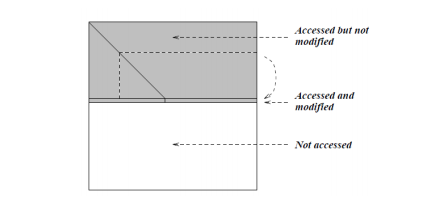
\includegraphics[width=0.5\linewidth]{figures/Figure_6.png}  %插入的图,包括JPG,PNG,PDF,EPS等,放在源文件目录下
	\caption{}  %图片的名称
	\label{fig:mcmthesis-logo}   %标签,用作引用
\end{figure}


思考:如果数据按列存储, 如 FORTRAN/MATLAB, 如何设计算法?	


\subsubsection{待定系数法计算 LU 分解}

设 $A = LU$, 即

{$\left[\begin{array}{ccccc}{a_{11}} & {a_{12}} & {a_{13}} & {\cdots} & {a_{1 n}} \\ {a_{21}} & {a_{22}} & {a_{23}} & {\cdots} & {a_{2 n}} \\ {a_{31}} & {a_{32}} & {a_{33}} & {\cdots} & {a_{3 n}} \\ {\vdots} & {} & {} & {\ddots} & {\vdots} \\ {a_{n 1}} & {a_{x 2}} & {a_{x 3}} & {\cdots} & {a_{n n}}\end{array}\right]$ =$\left[\begin{array}{cccc}{1} & {} & {} & {} \\ {l_{21}} & {1} & {} & {} \\ {l_{31}} & {l_{32}} & {1} & {} \\ {\vdots} & {} & {} & {\ddots} \\ {l_{n 1}} & {l_{n 2}} & {\cdots} & {l_{n, n-1}}\end{array}\right]$ $\left[\begin{array}{ccccc}{u_{11}} & {u_{12}} & {u_{13}} & {\cdots} & {u_{1 n}} \\ {} & {u_{22}} & {u_{23}} & {\cdots} & {u_{2 n}} \\ {} & {} & {u_{33}} & {\cdots} & {u_{2 n}} \\ {} & {} & {} & {\ddots} & {\vdots} \\ {} & {} & {} & {} & {u_{n n i}}\end{array}\right] $}

\noindent(1)比较等式两边的第一行, 可得

$u_{1 j}=a_{1 j}, \quad j=1,2, \dots, n$

再比较等式两边的第一列, 可得

$a_{i 1}=l_{i 1} u_{11} \Rightarrow l_{i 1}=a_{i 1} / u_{11}, \quad i=2,3, \ldots, n$

\noindent(2) 比较等式两边的第二行, 可得

$a_{2 j}=l_{21} u_{1 j}+a_{2 j} \Rightarrow u_{2 j}=a_{2 j}-l_{21} u_{1 j}, \quad j=2,3, \ldots, n$

再比较等式两边的第二列, 可得

$a_{i 2}=l_{i 1} u_{12}+l_{i 2} u_{22} \Rightarrow l_{i 1}=\left(a_{i 2}-l_{i 1} u_{12}\right) / u_{22}, \quad i=3,4, \ldots, n$

\noindent(3) 以此类推, 第 k 步时, 比较等式两边的第 k 行, 可得

$u_{k j}=a_{k j}-\left(l_{k 1} u_{1 j}+\cdots+l_{k, k-1} u_{k-1, j}\right), \quad j=k, k+1, \ldots, n$

比较等式两边的第 k 列, 可得

$l_{i k}=\left(a_{i k}-l_{i 1} u_{1 k}-\cdots-l_{i, k-1} u_{k-1, k}\right) / u_{k k}, \quad i=k+1, k+2, \ldots, n$

直到第 n 步, 即可计算出 L 和 U 的所有元素.

同样, 我们可以利用 A 来存储 L 和 U. 算法描述如下:
\begin{table}  
	%\caption{设置表格总长}  
	\begin{tabular*}{16cm}{ll}  
		\hline  
		算法 4.5 &LU 分解 (待定系数法或 $Doolittle$ 方法)\\  
		\hline  
		1:   & for k = 1 to n do\\  
		2:   & \qquad $a_{k j}=a_{k j}-\sum_{i=1}^{k-1} a_{k i} a_{i j}, \quad j=k, k+1, \ldots, n$\\
		3:   & \qquad $a_{i k}=\frac{1}{a_{k k}}\left(a_{i k}-\sum_{j=1}^{k-1} a_{i j} a_{j k}\right), \quad i=k+1, k+2, \ldots, n$\\
		4:   & end for\\
		\hline  
	\end{tabular*}  
\end{table} 

\begin{lstlisting}[language={[ANSI]C}] 
% Matlab code 3 : 待定系数法 LU 分解
function A = mylu2(A)
[n,n]=size(A);
for k=1:n
A(k,k)=A(k,k)-A(k,1:k-1)*A(1:k-1,k);
if (A(k,k)==0)
fprintf('Error: A(%d,%d)=0!\n', i,i);
return;
end
A(k,k+1:n)=A(k,k+1:n)-A(k,1:k-1)*A(1:k-1,k+1:n);
A(k+1:n,k)=A(k+1:n,k)-A(k+1:n,1:k-1)*A(1:k-1,k);
A(k+1:n,k)=A(k+1:n,k)/A(k,k);
end
\end{lstlisting}

\subsubsection{三角方程求解}
得到 $A$ 的 $LU$ 分解后, 我们最后需要用回代法求解两个三角方程组
$$L y=b, \quad U x=y$$

\begin{table}  
	%\caption{设置表格总长}  
	\begin{tabular*}{16cm}{ll}  
		\hline  
		算法 4.6 &向前回代求解$Ly =b$(假定$L$是一般的非奇异下三角矩阵)\\  
		\hline  
		1:   &$y_{1}=b_{1} / l_{11}$\\  
		2:   & for i = 2 : n do\\
		3:   & \qquad for j = 1 : i − 1 do\\
		4:    & \qquad \qquad$b_{i}=b_{i}-l_{i j} y_{j}$\\
		5:   & \qquad end for\\
		6:    & \qquad $y_{i}=b_{i} / l_{i i}$\\
		7:    & end for\\
		\hline  
	\end{tabular*}  
\end{table}

如果数据是按列存储的, 则采用列存储方式效率会高一些.

下面是按列存储方式求解上三角方程组.

\begin{table}  
	%\caption{设置表格总长}  
	\begin{tabular*}{16cm}{ll}  
		\hline  
		算法 4.7 &向前回代求解$Ly =b$(假定$L$是一般的非奇异下三角矩阵)\\  
		\hline  
		1:   & for i = n : −1 : 1 do\\  
		2:   & \qquad $x_{i}=y_{i} / u_{i i}$\\
		3:   & \qquad for j = i − 1 : −1 : 1 do\\
		4:    & \qquad \qquad$y_{j}=y_{j}-x_{i} u_{j i}$\\
		5:   & \qquad end for\\
		6:    & end for\\
		\hline  
	\end{tabular*}  
\end{table}

这两个算法的运算量均为$n^2+O(n)$

\subsubsection{选主元 LU 分解}
• 在 LU 分解算法 1.2 中, 我们称 $a_{k k}^{(k-1)}$ 为主元. 如果 $a_{k k}^{(k-1)}=0$, 则算法就无法进行下去.

• 即使 $a_{k k}^{(k-1)}$ 不为零, 但如果$\left|a_{k k}^{(k-1)}\right|$ 的值很小, 由于舍入误差的原因,也可能会给计算结果带来很大的误差.

• 此时我们就需要通过 选主元 来解决这个问题.


{例} 用 LU 分解求解线性方程组 Ax = b, 其中
\begin{equation}
A=\left[\begin{array}{cc}{0.02} & {61.3} \\ {3.43} & {-8.5}\end{array}\right], \quad b=\left[\begin{array}{c}{61.5} \\ {25.8}\end{array}\right]
\end{equation}

要求在运算过程中保留 3 位有效数字.	

$(x_1 ≈ −20.7, x_2 ≈ 1.01)$


易知, 方程的精确解为 $x_1 = 10.0$ 和 $x_2 = 1.00$. 我们发现 $x_1$ 的误差非常
大. 导致这个问题的原因就是 $|a_{11}| $太小, 用它做主元时会放大舍入误差.
所以我们需要选主元.

\subsection{选主元 LU 分解}

\begin{theorem}
	设 $A ∈ R^{n×n}$ 非奇异, 则存在置换矩阵 $P_L$,$ P_R$, 以及单位下三角
	矩阵 $L$ 和非奇异上三角矩阵 $U$, 使得 $P_LAP_R = LU$. 其中 $P_L$ 和 $P_R$ 中只有一个是必需的.
\end{theorem}


第 $k$ 步时, 如何选取置换矩阵 $P^{(k)}_L$ 和 $P^{(k)}_R$ ?

选法一. 选取 $P^{(k)}_L$ 和 $P^{(k)}_R$ 使得主元为剩下的矩阵中绝对值最大, 这种选
取方法称为 “全主元 $Gauss$ 消去法”, 简称 $GECP$ (Gaussian elimination
with complete pivoting);

选法二. 选取 $P^{(k)}_L$ 和$ P^{(k)}_R$ 使得主元为第 $k$ 列中第 $k$ 到第 $n$ 个元素中, 绝对值最大, 这种选取方法称为 “部分选主元 $Gauss$ 消去法”, 简称 $GEPP$
(Gaussian elimination with partial pivoting), 此时 $P^{(k)}_R = I$, 因此也称为列主元 $Gauss$ 消去法.


† (1) $GECP$ 比 $GEPP$ 更稳定, 但工作量太大, 在实际应用中通常使用$GEPP$ 算法.

(2) $GEPP$ 算法能保证$L$ 所有的元素的绝对值都不超过 $1$.


\begin{table}  
	%\caption{设置表格总长}  
	\begin{tabular*}{16cm}{ll}  
		\hline  
		算法 4.7 &向前回代求解$Ly =b$(假定$L$是一般的非奇异下三角矩阵)\\  
		\hline  
		1:   & p = 1 : n \% 用于记录置换矩阵\\  
		2:   & for k = 1 to n − 1 do\\
		3:   & \qquad $\left[a_{\max }, l\right]=\max _{k \leq i \leq n}\left|a_{i k}\right|$ \% 选列主元, 其中 l 表示主元所在的行 \\
		4:    & \qquad if l ̸= k then\\
		5:   & \qquad \qquad for j = 1 to n do\\
		6:    & \qquad \qquad \qquad $t m p=a_{k j}, a_{k j}=a_{l j}, a_{l j}=\operatorname{tm} p$ \% 交换第 k 行与第l 行\\
		7:    &\qquad \qquad end for\\
		8:   & \qquad \qquad $\operatorname{tm} p=p(k), p(k)=p(l), p(l)=\operatorname{tm} p$ \%更新置换矩阵 \\
		9:   & \qquad end if\\
		10:   & \qquad for i = k + 1 to n do\\
		11:   & \qquad \qquad $a_{i k}=a_{i k} / a_{k k}$ \%计算 L 的第 k 列\\
		12:   & \qquad end for\\
		13:   & \qquad for i = k + 1 to n do\\
		14:   & \qquad \qquad for j = k + 1 to n do\\
		15:   & \qquad \qquad \qquad $a_{i j}=a_{i j}-a_{i k} * a_{k j}$ \%更新 A(k + 1 : n, k + 1 : n) \\
		16:   & \qquad \qquad end for \\
		17:   & \qquad end for \\
		18:    & end for \\
		\hline  
	\end{tabular*}  
\end{table}

\begin{lstlisting}[language={[ANSI]C}] 
% Matlab code 2 : 部分选主元 LU 分解
function [A,p] = myplu(A)
[n,n]=size(A); p=1:n;
for i=1:n-1
[a,k]=max(abs(A(i:n,i)));
if a==0
error('Error: 第 %d 步的列主元为 0!\n', i);
end
k=k+i-1;
if k~=i
tmp=A(i,:); A(i,:)=A(k,:); A(k,:)=tmp;
tmp=p(i); p(i)=p(k); p(k)=tmp;
end
A(i+1:n,i)=A(i+1:n,i)/A(i,i);
A(i+1:n,i+1:n)=A(i+1:n,i+1:n)-A(i+1:n,i)*A(i,i+1:n);
end
\end{lstlisting}


{例} 用 LU 分解求解线性方程组 Ax = b, 其中
\begin{equation}
A=\left[\begin{array}{cc}{0.02} & {61.3} \\ {3.43} & {-8.5}\end{array}\right], \quad b=\left[\begin{array}{c}{61.5} \\ {25.8}\end{array}\right]
\end{equation}

要求在运算过程中保留 3 位有效数字.	

$(x_1 ≈ 10.0, x_2 ≈ 0.998)$


\subsubsection{矩阵求逆}
我们可以通过部分选主元 $LU$ 分解来计算矩阵的逆. 设 $P A = LU$, 则

$$
A^{-1}=P^{T} U^{-1} L^{-1}
$$

等价于求解下面 $2n$ 个三角线性方程组

$$
L y_{i}=P e_{i}, \quad U x_{i}=y_{i}, \quad i=1,2, \ldots, n
$$

也可以分别计算 $L^{-1}$ 和 $U^{−1}$, 然后相乘. 哪种方法划算?

\subsection{特殊方程组的求解}

2.1 对称正定线性方程组

2.2 对称不定线性方程组

2.3 三对角线性方程组

2.4 带状线性方程组

2.5 Toeplitz 线性方程组

\subsubsection{对称正定线性方程组}

我们首先给出对称正定矩阵的几个基本性质.

\begin{theorem}
	设$ A ∈ \mathbb{R}^{n×n}$.
	• $A$ 对称正定当且仅当 $A$ 对称且所有特征值都是正的;
	
	• $A $对称正定当且仅当 $X^{⊺}AX$ 对称正定, 其中 $X ∈ \mathbb{R}^{n×n} $是一个任意的非奇异矩阵;
	
	• 若 $A$ 对称正定, 则 $A$ 的任意主子矩阵都对称正定;
	
	• 若 $A$ 对称正定, 则 $A$ 的所有对角线元素都是正的, 且
	$$
	\max _{i \neq j}\left\{\left|a_{i j}\right|\right\}<\max _{i}\left\{a_{i i}\right\}
	,$$即绝对值最大的元素出现在对角线上.
\end{theorem}


{\bfseries Cholesky 分解}


\begin{theorem}(Cholesky 分解)
	设 $A ∈ \mathbb{R}^{n×n}$ 对称正定, 则存在唯一的对角线元
	素为正的下三角矩阵$ L$, 使得
	$$
	A=L L^{\top}
	$$
	该分解称为 $Cholesky$ 分解.	
\end{theorem}


{\bfseries Cholesky 分解的实现}
设 $A = LL^{⊺}$, 即
\begin{equation}
\left[\begin{array}{cccc}{a_{11}} & {a_{12}} & {\cdots} & {a_{1 n}} \\ {a_{21}} & {a_{22}} & {\cdots} & {a_{2 n}} \\ {\vdots} & {} & {\ddots} & {\vdots} \\ {a_{n 1}} & {a_{n 2}} & {\cdots} & {a_{n n}}\end{array}\right]=\left[\begin{array}{cccc}{l_{11}} & {} & {} & {} \\ {l_{21}} & {l_{22}} & {} & {} \\ {\vdots} & {\vdots} & {\ddots} & {} \\ {l_{n 1}} & {l_{n 2}} & {\cdots} & {l_{n n}}\end{array}\right]\left[\begin{array}{cccc}{l_{11}} & {l_{21}} & {\cdots} & {l_{n 1}} \\ {} & {l_{22}} & {\cdots} & {l_{n 2}} \\{}& {} & {\ddots} & {\vdots} \\{} &{} & {} & {l_{n n}}\end{array}\right]
\end{equation}

直接比较等式两边的元素可得
\begin{equation}
a_{i j}=\sum_{k=1}^{n} l_{i k} l_{j k}=l_{j j} l_{i j}+\sum_{k=1}^{j-1} l_{i k} l_{j k}, \quad i, j=1,2, \ldots, n
\end{equation}

根据上面的计算公式, 可得下面的算法:

\begin{table}  
	%\caption{设置表格总长}  
	\begin{tabular*}{16cm}{ll}  
		\hline  
		算法 4.8 & Cholesky 分解算法\\  
		\hline  
		1:   & for j = 1 to n do\\  
		2:   & \qquad $l_{j j}=\left(a_{j j}-\sum_{k=1}^{j-1} l_{j k}^{2}\right)^{1 / 2}$\\
		3:   & \qquad for i = j + 1 to n do\\
		4:    & \qquad \qquad$l_{i j}=\left(a_{i j}-\sum_{k=1}^{j-1} l_{i k} l_{j k}\right) / l_{j j}$\\
		5:   & \qquad end for\\
		6:    & end for\\
		\hline  
	\end{tabular*}  
\end{table}

{\bfseries 几点说明}

• 与 $LU$ 分解一样, 可以利用 $A$ 的下三角部分来存储 $L$;

• $Cholesky$ 分解算法的运算量为$\frac{1}{3} n^{3}+O\left(n^{2}\right)$, 大约为 $LU$ 分解的一半;

• $Cholesky$ 分解算法是稳定的(稳定性与全主元 $Gauss$ 消去法相当),
故不需要选主元.

{\bfseries 改进的 Cholesky 分解算法}
为了避免开方运算, 我们可以将 $A$ 分解为: $A = LDL^{\top}$, 即
\begin{equation}
\left[\begin{array}{cccc}{a_{11}} & {a_{12}} & {\cdots} & {a_{1 n}} \\ {a_{21}} & {a_{22}} & {\cdots} & {a_{2 n}} \\ {\vdots} & {} & {\ddots} & {\vdots} \\ {a_{n 1}} & {a_{n 2}} & {\cdots} & {a_{n n}}\end{array}\right]=\left[\begin{array}{cccc}{1} & {} & {} & {} \\ {l_{21}} & {1} & {} & {} \\ {\vdots} & {} & {\ddots} & {} \\ {l_{n 1}} & {\cdots} & {l_{n, n-1}} & {1}\end{array}\right]\left[\begin{array}{cccc}{d_{1}} & {} & {} & {} \\ {} & {d_{2}} & {} & {} \\ {} & {} & {\ddots} & {} \\ {} & {} & {} & {d_{n}}\end{array}\right]\left[\begin{array}{cccc}{1} & {l_{21}} & {\cdots} & {l_{n 1}} \\ {1} & {\cdots} & {l_{n 2}} \\ {} & {\ddots} & {\vdots} \\ {} & {} & {1}\end{array}\right]
\end{equation}

通过待定系数法可得
\begin{equation}
a_{i j}=\sum_{k=1}^{n} l_{i k} d_{k} l_{j k}=d_{j} l_{i j}+\sum_{k=1}^{j-1} l_{i k} d_{k} l_{j k}, \quad i, j=1,2, \ldots, n
\end{equation}

基于以上分解来求解对称正定线性方程组的算法称为改进的平方根法:
\begin{table}  
	%\caption{设置表格总长}  
	\begin{tabular*}{16cm}{ll}  
		\hline  
		算法 4.9 &改进的平方根法\\  
		\hline  
		1:   & for j = 1 to n do \% 先计算分解\\  
		2:   & \qquad $d_{j}=a_{j j}-\sum_{k=1}^{j-1} l_{j k}^{2} d_{k}$\\
		3:   & \qquad for i = j + 1 to n do \\
		4:    & \qquad $l_{i j}=\left(a_{i j}-\sum_{k=1}^{j-1} l_{i k} d_{k} l_{j k}\right) / d_{j}$\\
		5:   & \qquad end for\\
		6:    & end for\\
		7:    & $y_1 = b_1$ \% 解方程组: Ly = b 和 $DL^{\top}x = y$\\
		8:   & for i = 2 to n do \\
		9:   & \qquad $y_{i}=b_{i}-\sum_{k=1}^{i-1} l_{i k} y_{k}$\\
		10:   & end for\\
		11:   & $x_{n}=y_{n} / d_{n}$\\
		12:   & for i = n − 1 to 1 do\\
		13:   & \qquad $x_{i}=y_{i} / d_{i}-\sum_{k=i+1}^{n} l_{k i} x_{k}$\\
		14:   & end for\\
		\hline  
	\end{tabular*}  
\end{table}

\subsubsection{对称不定线性方程组}

$A → $非奇异, 对称不定

若 $A$ 存在 $LU$ 分解, 即 $A = LU$, 则可写成 $A = LDL^{\top}$

然而, 当 $A$ 不定时, 其 $LU$ 分解不一定存在.

若采用选主元 $LU$ 分解, 则其对称性将被破坏. 为了保持对称性, 在选主元
时必须对行列进行同样的置换, 即选取置换矩阵 $P$, 使得

\begin{equation}
P A P^{\top}=L D L^{\top}
\end{equation}

通常称 (2.4) 为对称矩阵的 $LDL^{\top}$ 分解.

不幸的是, 这样的置换矩阵可能不一定存在, 即分解 (2.4) 不一定存在.



{\bfseries 例} 设对称矩阵

\begin{equation}
A=\left[\begin{array}{lll}{0} & {1} & {1} \\ {1} & {0} & {1} \\ {1} & {1} & {0}\end{array}\right]
\end{equation}

由于 $A$ 的对角线元素都是 $0$, 对任意置换矩阵 $P$, 矩阵 $P AP^{\top}$ 的对角线
元素仍然都是 $0$. 因此, 矩阵 $A$ 不存在 $LDL^{\top}$ 分解.



{\bfseries Aasen 算法}

1971 年, Aasen 提出了下面的分解

\begin{equation}
P A P^{\top}=L T L^{\top}
\end{equation}

其中 $P$ 为置换矩阵, $L$ 为单位下三角矩阵, $T$ 为对称三对角矩阵.

分解 (2.5) 本质上与部分选主元 LU 分解是一样的.

{\bfseries 块 $LDL^{\top}$ 分解} 

设 $A$ 对称非奇异, 则存在置换矩阵 $P$ 使得
\begin{equation}
P A P^{\top}=\left[\begin{array}{cc}{B} & {E^{\top}} \\ {E} & {C}\end{array}\right]
\end{equation}
其中 $B ∈ \mathbb{R}$ 或 $B ∈ \mathbb{R}^{2×2}$
, 且非奇异. 因此可以对 $P AP^{\top}$ 进行块对角化, 即

\begin{equation}
P A P^{\top}=\left[\begin{array}{cc}{I} & {0} \\ {E B^{-1}} & {I}\end{array}\right]\left[\begin{array}{cc}{B} & {0} \\ {0} & {C-E B^{-1} E^{\top}}\end{array}\right]\left[\begin{array}{cc}{I} & {B^{-1} E^{\top}} \\ {0} & {I}\end{array}\right]
\end{equation}

其中$C-E B^{-1} E^{\top}$是$Schur$补。

不断重复以上过程, 就可以得到 A 的块 $LDL^{\top}$ 分解:
\begin{equation}
P A P^{\top}=L \tilde{D} L^{\top}
\end{equation}
其中$\tilde{D}$是拟对角矩阵, 即块对角矩阵且对角块的大小为 1 或 2

{\bfseries 选主元块 $LDL^{\top}$ 分解}
与选主元 $LU$ 分解类似, 我们需要考虑块 $LDL^{\top}$ 分解的选主元策略, 即如何
选取置换矩阵. 目前常用的策略有

• 全主元策略: 由 $Bunch$ 和 $Parlett$ 于 1971 年提出, 并证明了其稳定性.
但需要进行 $n^3/6$ 次比较运算, 代价比较昂贵.

• 部分选主元策略: 由 $Bunch$ 和 $Kaufman$ 于 1977 年提出, 将比较运算
复杂度降低到 $O(n^2)$ 量级, 而且具有较满意的向后稳定性. 因此被广
泛使用.

• Rook 策略: 由 Ashcraft, Grimes 和 Lewis 于 1998 年提出, 整体上与部
分选主元类似, 但在选主元时加了一层迭代, 从而能提供更高的精度

\begin{framed}
	目前大部分软件都采用部分选主元块 $LDL^{\top}$分解算法
\end{framed}

\subsubsection{三对角线性方程组}
\begin{equation}
A=\left[\begin{array}{cccc}{b_{1}} & {c_{1}} & {} & {} \\ {a_{1}} & {\ddots} & {\ddots} & {} \\ {} & {\ddots} & {\ddots} & {c_{n-1}} \\ {} & {} & {a_{n-1}} & {b_{n}}\end{array}\right]
\end{equation}
我们假定

\begin{equation}
\left|b_{1}\right|>\left|c_{1}\right|>0, \quad\left|b_{n}\right|>\left|a_{n-1}\right|>0
\end{equation}
\begin{equation}
\left|b_{i}\right| \geq\left|a_{i-1}\right|+\left|c_{i}\right|, \quad a_{i} c_{i} \neq 0, \quad i=1, \ldots, n-1
\end{equation}

即 A 是 不可约弱对角占优


如果 A 可约, 怎么处理?


此时, 我们可以得到下面的三角分解
\begin{equation}
A=\left[\begin{array}{cccc}{b_{1}} & {c_{1}} & {} & {} \\ {a_{1}} & {\ddots} & {\ddots} & {} \\ {} & {\ddots} & {\ddots} & {c_{n-1}} \\ {} & {} & {a_{n-1}} & {b_{n}}\end{array}\right]=\left[\begin{array}{cccc}{\alpha_{1}} & {} & {} & {} \\ {a_{1}} & {\alpha_{2}} & {} & {} \\ {} & {\ddots} & {\ddots} & {} \\ {} & {} & {a_{n-1}} & {\alpha_{n}}\end{array}\right]\left[\begin{array}{cccc}{1 \beta_{1}} \\ {1} & {\ddots} \\ {} & {\ddots} & {\beta_{n-1}} \\ {} & {} & {1}\end{array}\right] \triangleq L U
\end{equation}

递推公式:
\begin{equation}
\begin{array}{l}{\alpha_{1}=b_{1}} 
\\ {\beta_{1}=c_{1} / \alpha_{1}=c_{1} / b_{1}} 
\\ {\left\{\begin{array}{l}{\alpha_{i}=b_{i}-a_{i-1} \beta_{i-1}} \\ {\beta_{i}=c_{i} / \alpha_{i}=c_{i} /\left(b_{i}-a_{i-1} \beta_{i-1}\right), \quad i=2,3, \ldots, n-1} \end{array}\right.}\\ {\alpha_{n}=b_{n}-a_{n-1} \beta_{n-1}}\end{array}
\end{equation}

为了使得算法能够顺利进行下去, 我们需要证明$\alpha_{i} \neq 0$


\begin{theorem}
	设三对角矩阵 A 满足条件 (2.6) 和 (2.7). 则 A 非奇异, 且
	
	(1)$\left|\alpha_{1}\right|=\left|b_{1}\right|>0$
	
	(2) $0<\left|\beta_{i}\right|<1, i=1,2, \ldots, n-1$
	
	(3)	$0<\left|c_{i}\right| \leq\left|b_{i}\right|-\left|a_{i-1}\right|<\left|\alpha_{i}\right|<\left|b_{i}\right|+\left|a_{i-1}\right|, i=2,3, \ldots, n$
\end{theorem}


\begin{table}  
	%\caption{设置表格总长}  
	\begin{tabular*}{16cm}{ll}  
		\hline  
		算法 4.9 &改进的平方根法\\  
		\hline  
		1:   & $\beta_{1}=c_{1} / b_{1}$\\  
		2:   & $y_{1}=f_{1} / b_{1}$\\
		3:   & : for i = 2 to n−1 do \\
		4:    & \qquad $\alpha_{i}=b_{i}-a_{i-1} \beta_{i-1}$\\
		5:   & \qquad $\beta_{i}=c_{i} / \alpha_{i}$\\
		6:    & \qquad $y_{i}=\left(f_{i}-a_{i-1} y_{i-1}\right) / \alpha_{i}$\\
		7:   & end for\\
		8:   & $\alpha_{n}=b_{n}-a_{n-1} \beta_{n-1}$ \\
		9:   & $y_{n}=\left(f_{n}-a_{n-1} y_{n-1}\right) / \alpha_{n}$\\
		10:  & $x_{n}=y_{n}$\\
		11:  & for i = n−1 to 1 do\\
		12:  & \qquad $x_{i}=y_{i}-\beta_{i} x_{i+1}$\\
		13:  & end for\\
		\hline  
	\end{tabular*}  
\end{table}


† 追赶法 (也称为 Thomas 算法) 的运算量大约为 $8n − 6$.



† 具体计算时, 由于求解 $Ly = f$ 与矩阵 $LU$ 分解是同时进行的, 因此,
$\alpha_i$ 可以不用存储. 但 $\beta_i$ 需要存储.



† 由于 $|\beta_i| < 1$, 因此在回代求解 $x_i$ 时, 误差可以得到有效控制.


需要指出的是, 我们也可以考虑下面的分解
\begin{equation}
A=\left[\begin{array}{cccc}{b_{1}} & {c_{1}} & {} & {} \\ {a_{1}} & {\ddots} & {\ddots} & {} \\ {} & {\ddots} & {\ddots} & {c_{n-1}} \\ {} & {} & {a_{n-1}} & {b_{n}}\end{array}\right]=\left[\begin{array}{ccccc}{1} \\ {\gamma_{1}} & {1} & {} & {} \\ {} & {\ddots} & {\ddots} & {} \\ {} & {} & {\gamma_{n-1}} & {1}\end{array}\right]\left[\begin{array}{cccc}{\alpha_{1}} & {c_{1}} & {} & {} \\ {} & {\alpha_{2}} & {\ddots} & {} \\ {} & {} & {\ddots} & {c_{n-1}} \\ {} & {} & {} & {\alpha_{n}}\end{array}\right]
\end{equation}

但此时$ |\gamma_i|$ 可能大于 1. 比如$ \gamma_1 = a_1/b_1$, 因此当$|b_1| < |a_1|$ 时, $|\gamma_1| > 1$.
所以在回代求解时, 误差可能得不到有效控制. 另外一方面, 计算$ γi$ 时也
可能会产生较大的舍入误差 (大数除以小数).

但如果 A 是列对角占优, 则可以保证$ |\gamma_i| < 1.$


† 如果 A 是 (行) 对角占优, 则采用前面的分解;

如果 A 是列对角占优, 则采用分解 (2.11).


\subsubsection{带状线性方程组}
设 $A ∈ R^{n×n}$ 是带状矩阵, 其下带宽为 $b_L$, 上带宽为$b_U$ , 即
\begin{equation}
a_{i j}=0 \quad \text { for } \quad i>j+b_{L} \text { or } i<j-b_{U}
\end{equation}

\begin{figure}[h]%%图
	\centering  %插入的图片居中表示
	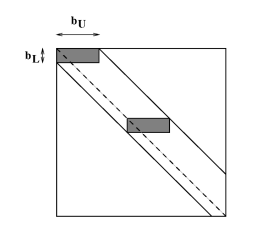
\includegraphics[width=0.7\linewidth]{figures/Figure_7.png}  %插入的图,包括JPG,PNG,PDF,EPS等,放在源文件目录下
	\caption{}  %图片的名称
	\label{fig:mcmthesis-logo}   %标签,用作引用
\end{figure}

对于带状矩阵, 其 LU 分解有如下性质:

\begin{theorem}
	设 $A ∈ R^{n×n}$ 是带状矩阵, 其下带宽为 $b_L$, 上带宽为 $b_U$ . 若 $A =
	L_U$ 是不选主元的 $L_U$ 分解, 则 $L$ 为下带宽为 $b_L$ 的带状矩阵, $U$ 为上带
	宽为 $b_U$ 的带状矩阵.	
\end{theorem}


统计求解带状矩阵 $Ax = b$ 的运算量.

若采用部分选主元的 LU 分解, 则有

\begin{theorem}
	设 $A ∈ R
	n×n $是带状矩阵, 其下带宽为$ b_L$, 上带宽为 $b_U$ . 若 $P A =
	LU $是部分选主元的 $LU$ 分解, 则 $U$ 为上带宽不超过$b_L + b_U$ 的带状矩
	阵, $L $为下带宽为 $b_L$ 的 “基本带状矩阵”, 即 L 每列的非零元素不超过
	$b_L + 1$ 个.
\end{theorem}


\subsubsection{Toeplitz 线性方程组}
\begin{equation}
T_{n}=\left[\begin{array}{cccc}{t_{0}} & {t_{-1}} & {\cdots} & {t_{-n+1}} \\ {t_{1}} & {\ddots} & {\ddots} & {\vdots} \\ {\vdots} & {\ddots} & {\ddots} & {t_{-1}} \\ {t_{n-1}} & {\cdots} & {t_{1}} & {t_{0}}\end{array}\right]
\end{equation}
$T_n$ 是反向对称 (persymmetric) 矩阵. 记 $J_n $为$ n$ 阶反向单位矩阵:
\begin{equation}
J_{n}=\left[\begin{array}{cccc}{ } & { } & { } &{1} \\{ } & { } &{1} & { } \\ {} & {\cdots}& { } & { } \\ {1} &{ } &{ } &{ }\end{array}\right]
\end{equation}
易知$J_{n}^{\top}=J_{n}^{-1}=J_{n}$


\begin{lemma}
	矩阵$ A ∈ \mathbb{R}^{n×n}$ 是反向对称矩阵当且仅当
	\begin{equation}
	A=J_{n} A^{\top} J_{n} \quad \text { 或 } \quad J_{n} A=A^{\top} J_{n}
	\end{equation}
\end{lemma}


若 A 可逆, 则可得
\begin{equation}
A^{-1}=J_{n}^{-1}\left(A^{\top}\right)^{-1} J_{n}^{-1}=J_{n}\left(A^{-1}\right)^{\top} J_{n}
\end{equation}

即反向对称矩阵的逆也是反向对称矩阵.

† Toeplitz 矩阵的逆是反向对称矩阵, 但不一定是 Toeplitz 矩阵.


{\bfseries Yule-Walker 方程组}

假定 $T_n$ 对称正定, 考虑线性方程组
\begin{equation}
T_{n} x=-r_{n}
\end{equation}

其中 $r_n = [t_1, t_2, . . . , t_{n−1}, t_n]^{\top}$
. 这类线性方程组称为 $Yule-Walker$ 方程组,
其中 $t_n$ 为任意给定的实数.

由于 $T_n$ 对称正定, 所以 $t_0 > 0$. 因此我们可以对 $T_n$ 的对角线元素进行单位化. 不失一般性, 我们假定 $T_n$ 的对角线元素为 1, 即
\begin{equation}
T_{n}=\left[\begin{array}{cccc}{1} & {t_{1}} & {\cdots} & {t_{n-1}} \\ {t_{1}} & {\ddots} & {\ddots} & {\vdots} \\ {\vdots} & {\ddots} & {\ddots} & {t_{1}} \\ {t_{n-1}} & {\cdots} & {t_{1}} & {1}\end{array}\right]
\end{equation}

由于方程组右端项的特殊性, 我们可以通过递推来求解.

记$T_{k} x=-r_{k}$的解为$\mathcal{X}^{(k)}$.设$T_{k+1} x=-r_{k+1}$的解$x^{(k+1)}=\left[\begin{array}{c}{z^{(k)}} \\ {\alpha_{k}}\end{array}\right]$。

代入后可得递推公式:

\begin{equation}
\alpha_{k}=\frac{-t_{k+1}-r_{k}^{\top} J_{k} x^{(k)}}{1+r_{k}^{\top} x^{(k)}}, \quad z^{(k)}=x^{(k)}+\alpha_{k} J_{k} x^{(k)} \quad k=1,2, \ldots
\end{equation}


因此, 我们就可以从一阶 $Yule-Walker$ 方程出发, 利用递推公式 (2.13) 计算
$T_nx = −r_n $的解. 总的运算量 (乘法与加减运算) 大约为 $3n^2$
.

为了减少运算量, 我们引入一个变量$\beta_{k} \triangleq 1+r_{k}^{\top} x^{(k)}$,则:
\begin{equation}
\begin{aligned} \beta_{k+1} &=1+r_{k+1}^{\top} x^{(k+1)} \\ &=1+\left[r_{k}^{\top}, t_{k+1}\right]\left[\begin{array}{c}{x^{(k)}+\alpha_{k} J_{k} x^{(k)}} \\ {\alpha_{k}}\end{array}\right] \\ &=1+r_{k}^{\top} x^{(k)}+\alpha_{k}\left(t_{k+1}+r_{k}^{\top} J_{k} x^{(k)}\right) \\ &=\left(1-\alpha_{k}^{2}\right) \beta_{k} \end{aligned}
\end{equation}

总运算量降为 $2n^2$
. 这就是求解 Yule-Walker 方程组的 Durbin 算法.

\begin{table}  
	%\caption{设置表格总长}  
	\begin{tabular*}{16cm}{ll}  
		\hline  
		算法  &求解 Yule-Walker 方程组的 Durbin 算法\\  
		\hline  
		1:   & 输入数据: $t = [t_1, t_2, . . . , t_n]$ \% 注: 这里假定 t0 = 1\\  
		2:   & $x(1) = −t_1, β = 1, α = −t_1$\\
		3:   & for for k = 1 to n − 1 do \\
		4:    & \qquad $\beta=(1-\alpha^2)\beta$\\
		5:   & \qquad $\alpha=-\left(t_{k+1}-\sum_{i=1}^{k} t_{k+1-i} x(i)\right) / \beta$\\
		6:    & \qquad $x(1 : k)=x(1 : k)+\alpha x(k :-1 : 1)$\\
		7:   &$x(k+1)=\alpha$\\
		8:   & end for\\
		\hline  
	\end{tabular*}  
\end{table}


{\bfseries 一般右端项的对称正定 Toeplitz 线性方程组}

考虑一般右端项的方程组 $T_nx = b$ , 其中 $T_n$ 对称正定.

我们利用递推方法来求解: 假定 $x^{(k)}$ 和 $y^{(k)}$ 分别是下面两个方程组的解:

\begin{equation}
T_{k} x=\left[b_{1}, b_{2}, \ldots, b_{k}\right]^{\top}, \quad T_{k} y=-\left[t_{1}, t_{2}, \ldots, t_{k}\right]^{\top}
\end{equation}

设$x^{(k+1)}=\left[\begin{array}{c}{z^{(k)}} \\ {\mu_{k}}\end{array}\right]$是$T_{k+1} x=b^{(k+1)}$的解,则可得

\begin{equation}
z^{(k)}=x^{(k)}+\mu_{k} J_{k} y^{(k)}, \quad \mu_{k}=\frac{b_{k+1}-r_{k}^{\top} J_{k} x^{(k)}}{1+r_{k}^{\top} y^{(k)}}
\end{equation}

所以, 我们可以先计算$T_{k} x=b^{(k)}$和$T_{k} x=-r_{k}$的解,, 然后利用上述公式得到$T_{k+1} x=b^{(k+1)}$的解,这就是 Levinson 算法, 总运算量大约为 $4n^2$.

\begin{table}  
	%\caption{设置表格总长}  
	\begin{tabular*}{16cm}{ll}  
		\hline  
		算法 4.9 &求解对称正定 Toeplitz 线性方程组的 Levinson 算法\\  
		\hline  
		1:   & 输入数据: $t = [t_1, t_2, . . . , t_n]$ \%假定 t0 = 1\\  
		2:   & $y(1) = −t_1, x(1) = b_1, \beta=1,\alpha = −t_1$\\
		3:   & for k = 1 to n−1 do \\
		4:    & \qquad $\beta=(1-\alpha^2)\beta$\\
		5:    & \qquad $\mu=\left(b_{k+1}-\sum_{i=1}^{k} t_{k+1-i} x(i)\right) / \beta$\\
		6:    & \qquad $x(1 : k)=x(1 : k)+\mu y(k :-1 : 1), \quad x(k+1)=\mu$\\
		7:    &\qquad if k < n − 1 then\\
		8:   & \qquad \qquad $\alpha=-\left(t_{k+1}+\sum_{i=1}^{k} t_{k+1-i} y(i)\right) / \beta$\\
		9:    &\qquad \qquad $y(1 : k)=y(1 : k)+\alpha y(k :-1 : 1)$\\
		10:   &\qquad \qquad $y(k + 1) = \alpha$\\
		11:   & \qquad end for \\
		12:   &end for\\
		\hline  
	\end{tabular*}  
\end{table}

在数学与工程的许多应用中都会出现 $Toeplitz$ 线性方程组. $Levinson$ 算法
是较早的关于对称正定 $Toeplitz$ 线性方程组的快速算法, 但并不稳定 (只
具有弱稳定性). 后来人们提出了各种各样的快速和超快速算法:

\begin{table}[h] %开始一个表格environment,表格的位置是h,here。  
	\caption{改变表格任一列宽} %显示表格的标题  
	\begin{tabular}{p{3.5cm}|p{2cm}|p{5cm}} %设置了每一列的宽度,强制转换。  
		\hline  
		\hline  
		方法 & 运算量 & 存储量 \\ %用&来分隔单元格的内容 \\表示进入下一行  
		\hline %画一个横线,下面的就都是一样了,这里一共有4行内容  
		Fast stable & $≥ 20n^2$& $≥ n^2/2$\\  
		\hline  
		Fast but unstable & $≥ 3n^2$ & $≥ 4n$\\  
		\hline  
		Superfast and “unstable” & $O(n log^2n) $& O(n)\\  
		\hline  
		Superfast preconditioner & O(n log n) & O(n)\\  
		\hline  
		\hline  
	\end{tabular}  
\end{table} 

• Fast : Levinson-Durbin (1946), Trench (1964), ...

• Fast stable: Bareiss (1969), Gohberg, Kailath and Olshevsky (1995), Chandrasekaran and Sayed (1998), Gu (1998), ...

• Superfast: Brent, Gustavson and Yun (1980), Bitmead and Anderson (1980),Morf (1980), de Hoog (1987), Ammar and Gragg (1988), ...

• Superfast Preconditioners: Strang, Chan, Chan, Tyrtyshnikov, ...
6


\subsection{扰动分析}

3.1 $δx$ 与 $\hat{x}$ 的关系

3.2 $δx$ 与 $x_∗$ 的关系

3.3 $δx$ 与残量的关系

3.4 相对扰动分析


考虑线性方程组
\begin{equation}
A x=b
\end{equation}
设 $x∗$ 是精确解, $\hat{x}$ 是通过数值计算得到的近似解. 假定$ \hat{x}$ 满足线性方程组
\begin{equation}
(A+\delta A) \hat{x}=b+\delta b
\end{equation}
$\delta x \triangleq \hat{x}-x$的大小, 即向后误差分析.

\subsubsection{$δx$ 与 $\hat{x}$ 的关系}

\begin{theorem}
	设 $||.||$任一向量范数(当该范数作用在矩阵上时就是相应的
	导出范数), 则 $δx $与 $\hat{x}$ 满足下面的关系式
	\begin{equation}
	\frac{\|\delta x\|}{\|\hat{x}\|} \leq\left\|A^{-1}\right\| \cdot\|A\|\left(\frac{\|\delta A\|}{\|A\|}+\frac{\|\delta b\|}{\|A\| \cdot\|\hat{x}\|}\right)
	\end{equation}
	当 $δb = 0$ 时, 有
	\begin{equation}
	\frac{\|\delta x\|}{\|\hat{x}\|} \leq \kappa(A) \frac{\|\delta A\|}{\|A\|}
	\end{equation}
\end{theorem}


\subsubsection{$δx$ 与 $x_{*}$ 的关系}

\begin{lemma}
	设 $||.||$是任一算子范数, $X ∈\mathbb{R}^{n×n}$. 若 $∥X∥ < 1,$ 则 I − X 可逆,且有
	\begin{equation}
	(I-X)^{-1}=\sum_{k=0}^{\infty} X^{k} \quad \text{和} \quad\left\|(I-X)^{-1}\right\| \leq \frac{1}{1-\|X\|}
	\end{equation}
\end{lemma}



\begin{theorem}
	设 $A ∈ R^{n×n}$ 非奇异且$\left\|A^{-1}\right\| \cdot\|\delta A\|<1$, 则
	\begin{equation}
	\frac{\|\delta x\|}{\left\|x_{*}\right\|} \leq \frac{\kappa(A)}{1-\kappa(A) \cdot \frac{\|\delta A\|}{\|A\|}}\left(\frac{\|\delta A\|}{\|A\|}+\frac{\|\delta b\|}{\|b\|}\right)
	\end{equation}
	
	如果 $||\delta A||=0$, 则
	\begin{equation}
	\frac{1}{\kappa(A)} \frac{\|\delta b\|}{\|b\|} \leq \frac{\|\delta x\|}{\left\|x_{*}\right\|} \leq \kappa(A) \frac{\|\delta b\|}{\|b\|}
	\end{equation}
\end{theorem}



\begin{theorem}
	设 $A ∈ \mathbb{R}^{n×n}$ 非奇异, 则有
	\begin{equation}
	\min \left\{\frac{\|\delta A\|_{2}}{\|A\|_{2}} : A+\delta A \text{奇异}\right\}=\frac{1}{\kappa_{2}(A)}
	\end{equation}
\end{theorem}



† 上述定理中的结论对所有 $p-$范数都成立.



† 度量
\begin{equation}
disp_p(A) \triangleq \min \left\{\frac{\|\delta A\|_{p}}{\|A\|_{p}} : A+\delta A \text{奇异}\right\}=\frac{1}{\kappa_{p}(A)}
\end{equation}	
表示 A 距离奇异矩阵集合的相对距离.


\subsubsection{$δx$ 与残量的关系}
记残量 (残差) 为$r=b-A \hat{x}$,则有
\begin{equation}
\delta x=\hat{x}-x_{*}=\hat{x}-A^{-1} b=A^{-1}(A \hat{x}-b)=-A^{-1} r
\end{equation}
所以可得
\begin{equation}
\|\delta x\| \leq\left\|A^{-1}\right\| \cdot\|r\|
\end{equation}
实际计算中 r 是可以计算的, 因此比较实用.

\subsubsection{相对扰动分析}
前面给出的误差 $\delta x$ 与条件数 $\kappa(A), \delta A$和 $\delta b$ 成比例. 许多情况下, 这个界
是令人满意的. 但有时相差很大, 不能很好的反映实际计算中解的误差.




{\bfseries 例} 设$A=\left[\begin{array}{ll}{\gamma} & {0} \\ {0} & {1}\end{array}\right], b=\left[\begin{array}{l}{\gamma} \\ {1}\end{array}\right]$,其中$\gamma > 1$,则$Ax = b$的精确解为
$x_{*}=\left[\begin{array}{l}{1} \\ {1}\end{array}\right]$,任何合理的直接法求得的解的误差都很小. 但系数矩阵的谱条件数为 $\kappa_{2}(A)=\gamma$,当$\gamma$很大时,$\kappa_{2}(A)$也很大, 因此误差界(2.16)和(2.18)可以是很大。

针对这个问题, 我们按分量进行分析. 记
\begin{equation}
\delta A=\left[\begin{array}{c}{\delta a_{11}} \\ {\delta a_{22}}\end{array}\right], \quad \delta b=\left[\begin{array}{c}{\delta b_{1}} \\ {\delta b_{2}}\end{array}\right]
\end{equation},

并设$\left|\delta a_{i j}\right| \leq \varepsilon\left|a_{i j}\right|,\left|\delta b_{i}\right| \leq \varepsilon\left|b_{i}\right|$,则
\begin{equation}
\delta x=\left[\begin{array}{c}{\hat{x}_{1}-x_{1}} \\ {\hat{x}_{2}-x_{2}}\end{array}\right]=\left[\begin{array}{c}{\frac{\delta b_{1}+b_{1}}{\delta a_{11}+a_{11}}-1} \\ {\frac{\delta b_{2}+b_{2}}{\delta a_{22}+a_{22}}-1}\end{array}\right]=\left[\begin{array}{c}{\frac{\delta b_{1}+\gamma}{\delta a_{11}+\gamma}-1} \\ {\frac{\delta b_{2}+1}{\delta a_{22}+1}-1}\end{array}\right]=\left[\begin{array}{c}{\frac{\delta b_{1}-\delta a_{11}}{\delta a_{11}+\gamma}} \\ {\frac{\delta b_{2}-\delta a_{22}}{\delta a_{22}+1}}\end{array}\right]
\end{equation}

故
\begin{equation}
\|\delta x\|_{\infty} \leq \frac{2 \varepsilon}{1-\varepsilon}
\end{equation}

如果 $δb = 0$, 则
\begin{equation}
\|\delta x\|_{\infty} \leq \frac{\varepsilon}{1-\varepsilon}
\end{equation}
这个界与 (2.16) 或 (2.18) 相差约 $\gamma$倍.


{\bfseries 相对条件数}

为了得到更好误差界, 我们引入相对条件数$\kappa_{cr}(A)$,即
\begin{equation}
\kappa_{c r}(A) \triangleq\left\|\left|A^{-1}\right| \cdot|A|\right\|
\end{equation}

有时也称为 Bauer 条件数或 Skeel 条件数.

假定 $δA$ 和 $δb$ 满足 $|δA| ≤ ε|A|$ 和 $|δb| ≤ ε|b|$. 由 $(A + δA)\hat{x} = b + δb $可得

\begin{equation}
\begin{aligned}|\delta x| &=\left|A^{-1}(-\delta A \hat{x}+\delta b)\right| \\ & \leq\left|A^{-1}\right| \cdot(|\delta A| \cdot|\hat{x}|+|\delta b|) \\ & \leq\left|A^{-1}\right| \cdot(\varepsilon|A| \cdot|\hat{x}|+\varepsilon|b|) \\ &=\varepsilon\left|A^{-1}\right| \cdot(|A| \cdot|\hat{x}|+|b|) \end{aligned}
\end{equation}

若 $δb = 0$, 则有
\begin{equation}
\|\delta x\|=\||\delta x|\| \leq \varepsilon\left\|\left|A^{-1}\right| \cdot|A| \cdot|\hat{x}|\right\| \leq \varepsilon\left\|\left|A^{-1}\right| \cdot|A|\right\| \cdot\|\hat{x}\|
\end{equation}

即
\begin{equation}
\frac{\|\delta x\|}{\|\hat{x}\|} \leq\left\|\left|A^{-1}\right| \cdot|A|\right\| \cdot \varepsilon=\kappa_{c r}(A) \cdot \varepsilon
\end{equation}

相对条件数有下面的性质

\begin{lemma}
	设$ A∈ R^{n×n}$非奇异,$D ∈ R^{n×n}$ 为非奇异对角矩阵, 则
	\begin{equation}
	\kappa_{c r}(D A)=\kappa_{c r}(A)
	\end{equation}
\end{lemma}



\begin{theorem}
	设$ A∈ R^{n×n}$非奇异,使得$|\delta A| \leq \varepsilon|A|,|\delta b| \leq \varepsilon|b|$成立,且满足
	\begin{equation}
	(A+\delta A) \hat{x}=b+\delta b
	\end{equation}
	的最小的 $ε > 0$ 称为按分量的相对向后误差, 其表达式为
	\begin{equation}
	\varepsilon=\max _{1 \leq i \leq n} \frac{\left|r_{i}\right|}{(|A| \cdot|\hat{x}|+|b|)_{i}}
	\end{equation},
	其中 $r = b − A\hat{x}$
\end{theorem}


更多关于数值计算的稳定性和矩阵扰动分析方面的知识, 可以参考相关
资料.

\subsection{误差分析}

4.1 LU 分解的舍入误差分析

4.2 Gauss 消去法的舍入误差分析

\subsubsection{LU 分解的舍入误差分析}
关于 LU 分解的舍入误差分析, 我们有下面的结果.

\begin{theorem}
	假定 $A ∈ \mathbb{R}^{n×n}$ 的所有顺序主子式都不为 $0$, 则带舍入误差的 $LU$分解可表示为
	\begin{equation}
	A=L U+E
	\end{equation}
	其中误差 E 满足
	\begin{equation}
	|E| \leq \gamma_{n}|L| \cdot|U|
	\end{equation}
	这里$\gamma_{n}=\frac{n \varepsilon_{u}}{1-n \varepsilon_{u}}, \varepsilon_{u}$表示机器精度.
\end{theorem}


\subsubsection{Gauss 消去法的舍入误差分析}

\begin{lemma}[High02] 设 $\hat{y}$ 和 $\hat{x}$ 分别是由向前回代和向后回代得到的数值解, 则
	\begin{equation}
	\begin{array}{ll}{(L+\delta L) \hat{y}=b,} & {|\delta L| \leq \gamma_{n}|L|} \\ {(U+\delta U) \hat{x}=\hat{y},} & {|\delta U| \leq \gamma_{n}|U|}\end{array}
	\end{equation}
\end{lemma}


该引理表明, 向前回代算法和向后回代算法都是稳定的.


† 在绝大多数情况下, 部分选主元 Gauss 消去法是向后稳定的, 但理论
上也存在失败的例子.



† 全主元 Gauss 消去法是数值稳定的. 在大部分实际应用中, 部分选主
元 Gauss 消去法与全主元 Gauss 消去法具有同样的数值稳定性.


\subsection{解的改进和条件数估计}

5.1 高精度运算

5.2 矩阵元素缩放 (Scaling)

5.3 迭代改进法

\subsubsection{高精度运算}
在计算中, 尽可能采用高精度的运算.

比如, 原始数据是单精度的, 但在计算时都采用双精度运算, 或者更高精度的运算. 但更高精度的运算会带来更大的开销.

\subsubsection{矩阵元素缩放 (Scaling)}
如果 A 的元素在数量级上相差很大, 则在计算过程中很可能会出现大数
与小数的加减运算, 这样就可能会引入更多的舍入误差. 为了避免由于这
种情况而导致的舍入误差, 我们可以在求解之前先对矩阵元素进行缩放
(Scaling), 即在矩阵两边同时乘以两个适当的对角矩阵.


{\bfseries 例} 考虑线性方程组
\begin{equation}
\left[\begin{array}{ccc}{-4000} & {2000} & {2000} \\ {2000} & {0.78125} & {0} \\ {2000} & {0} & {0}\end{array}\right]\left[\begin{array}{l}{x_{1}} \\ {x_{2}} \\ {x_{3}}\end{array}\right]=\left[\begin{array}{c}{400} \\ {1.3816} \\ {1.9273}\end{array}\right]
\end{equation}

用部分选主元 Gauss 法求解, 计算过程保留 8 位有效数字, 求得数值解
\begin{equation}
\overline{x}=[0.00096365,-0.698496,0.90042329]^{\top}
\end{equation}
与精确解$x=[1.9273 \cdots,-0.698496 \cdots, 0.9004233 \cdots]^{\top}$误差较大

考虑矩阵元素缩放, 即同乘对角阵  $D = diag(0.00005, 1, 1)$,得新方程组
\begin{equation}
D A D y=D b
\end{equation}
最后令$\tilde{x}=D y$, 即可求得比较精确的数值解.


\subsubsection{迭代改进法}
设近似解 $\hat{x}$, 残量$ r = b − A\hat{x}$. 当 $\hat{x}$ 没达到精度要求时, 可以考虑方程$Az = r$. 如果$ z $该方程的精确解, 则
\begin{equation}
A(\hat{x}+z)=A \hat{x}+A z=(b-r)+r=b
\end{equation}'
因此 $\hat{x} + z$ 就是原方程的精确解. 在实际计算中, 我们只能得到近似解 $\hat{z}$,
但 $||r-A\hat{z}||$很小, 特别地, 应该比 $||r||$更小. 因此$ \hat{x} + \hat{z}$ 应该比 $xˆ$ 更接近精确解.

如果新的近似解 $\hat{x} + \hat{z} $还不满足精度要求, 则可重复以上过程.
这就是通过迭代来提高解的精度.

\begin{table}  
	%\caption{设置表格总长}  
	\begin{tabular*}{16cm}{ll}  
		\hline  
		算法 5.1 &通过迭代改进解的精度\\  
		\hline  
		1:   & 设 $P A = LU, \hat{x}x$是 $Ax = b$ 的近似解\\  
		2:   & while 近似解 $\hat{x}$ 不满足精度要求, do\\
		3:   & \qquad 计算 $r = b -A \hat{x}$ \\
		4:    & \qquad 求解$Ly=Pr$,即$y=L^{-1}Pr$\\
		5:    & \qquad 求解$Uz=y$,即$z=U^{-1}y$\\
		6:    & \qquad 令$\hat{x}=\hat{x}+z$\\
		7:    &end while\\
		\hline  
	\end{tabular*}  
\end{table}

由于每次迭代只需计算一次残量和求解两个三角线性方程组, 因此运算
量为 $O(n^2)$. 所以相对来讲还是比较经济的.

† 为了提高计算精度, 在计算残量 $r$ 时最好使用原始数据 $A$, 而不是$P^{\top}LU$, 因此对 $A$ 做 $LU$ 分解时需要保留矩阵 $A$, 不能被 $L$ 和 $U$ 覆盖.

† 实际计算经验表明, 当 $A$ 病态不是很严重时, 即 $ε_uκ_∞(A) < 1$, 迭代
法可以有效改进解的精度, 最后达到机器精度. 但 $ε_uκ_∞(A) ≥ 1$ 时,
一般没什么效果. 这里 $ε_u$ 表示机器精度.

%%%%%%%%%%%%%%%%%%%%%%%%%%%%%%%%%%%%%%%%%%%%%%%%%%%%%%%%%
%%%                      第四章                        %%%
%%%%%%%%%%%%%%%%%%%%%%%%%%%%%%%%%%%%%%%%%%%%%%%%%%%%%%%%%
\chapter{最小二乘问题}
\begin{itemize}     
	\item[$\bullet$]线性最小二乘问题
	\item[$\bullet$]总体最小二乘问题
	\item[$\bullet$]约束最小二乘问题
	\item[$\bullet$]$\cdots$
\end{itemize}

最小二乘问题在统计学, 最优化问题, 材料与结构力学, 信号与图像处理等方面都有着广泛的应用, 是计算数学的一个重要研究分支, 也是一个活跃的研究领域.

本讲主要介绍求解\textcolor{blue}{线性最小二乘问题}的三种直接法.

\section{线性最小二乘问题}

\subsection{引言}
\noindent 考虑线性最小二乘问题
\begin{equation}
\min_{x\in\mathbb{R}} ||Ax-b||_2^2
\end{equation}
其中$A\in\mathbb{R}^{m\times n},b\in\mathbb{R}^m$.
问题(\textcolor{blue}{1})的解称为\textcolor{blue}{最小二乘解}.
\begin{itemize}
	\item[$\bullet$]当$m=n$且$A$非奇异时,这就是一个线性方程组,解为        $x=A^{-1}b$;
	\item[$\bullet$]当$m<n$时,未知量个数大于约束个数,此时我们称问题
	(\textcolor{blue}{1})为\textcolor{blue}{欠定}
	(或亚定)的
	\item[$\bullet$]当$m>n$时,约束个数大于未知量个数, 此时我们称问题
	(\textcolor{blue}{1})为\textcolor{blue}{超定}的
\end{itemize}

\noindent 为了讨论方便,本讲总是假定$A$是满秩的.
\subsubsection{欠定方程组}
若$m<n$,则$Ax=b$存在无穷多个解,这时我们通常寻求最小范数解, 于是问题就转化为下面的\textcolor{blue}{约束优化问题}
\begin{equation}
\min _{Ax=b} \frac{1}{2}\|x\|_{2}^{2}
\end{equation}

\noindent 对应的\textcolor{blue}{Lagrange函数}为$$\mathcal{L}(x, \lambda)=\frac{1}{2}\|x\|_{2}^{2}+\lambda^{\top}(A x-b)$$
其中$\lambda=\left[\lambda_{1}, \lambda_{2}, \ldots, \lambda_{m}\right]^{\top}$
是\textcolor{blue}{Lagrange乘子}.

此时优化问题(\textcolor{blue}{2})的解就是$\mathcal{L}(x,\lambda)$的\textcolor{blue}{鞍点},即下面
方程组的解:$$\frac{\partial \mathcal{L}}{\partial x}=x+{A}^{\top}
\lambda=0,\frac{\partial \mathcal{L}}{\partial \lambda}=Ax-b=0.$$
写成矩阵形式为$$
\left[\begin{array}{ll}{I} & {A^{\top}} \\ {A} &{0}\end{array}\right]\left[\begin{array}{l}{x} \\{\lambda}\end{array}\right]=\left[\begin{array}{l}{0} \\{b}\end{array}\right]
$$
如果$A$(行)满秩,即$rank(A)=m$,则系数矩阵非奇异, 上述方程组存在唯一解.

\subsubsection{超定方程组}
当$m>n$时,线性方程组$Ax=b$的解可能不存在.记$$J(x)=\|A x-b\|_{2}^{2}$$
易知$J(x)$是关于$x$的二次凸函数.因此,$x_*$是问题(\textcolor{blue}{1})的解当且仅当$x_*$是$J(x)$的
稳定点.

令其一阶导数为零, 可得$$A^{\top} A x-A^{\top} b=0$$
于是(1)就转化为一个(半正定)线性方程组.

本讲我们主要讨论超线性最小二乘问题的求解.
\subsection{初等变换矩阵}
矩阵计算的一个基本思想就是把较复杂的问题转化为等价的较简单的,
易于求解问题. 而完成这个转化的基本工具就是初等变换矩阵, 其中常用
的有三个: Gauss 变换, Householder 变换和 Givens 变换.

\subsubsection{初等矩阵}
\noindent 我们考虑\textcolor{blue}{初等矩阵}$$E(u, v, \tau)=I-\tau u v^*$$
其中$u,v\in \mathbb{C}^n$是非零向量,$\tau$是一个非零复数.事实上,$E(u,v,\tau)$是单位矩阵的一个秩1扰动.

\noindent \textcolor{blue}{定理}~~设$E(u,v,\tau)$是一个初等矩阵,我们有

(1)$\operatorname{det}(E(u, v, \tau))=1-\tau v^{*} u$

(2)若$1-\tau v^* u \neq 0$,则$E(u,v,\tau)$非奇异,且
$$(E(u,v,\tau))^{-1}=E(u,v,\tau)$$
其中$\gamma=\frac{\tau}{\tau v^{*} u-1}$

\subsubsection{Gauss变换}
\noindent 设$l_{j}=\left[0, \ldots, 0, l_{j+1, j}, \ldots, l_{n,
	j}\right]^{\top}, j=1,2, \ldots, n$,则\textcolor{blue}{Gauss变换}定义为$$
L\left(l_{j}\right) \triangleq E\left(l_{j}, e_{j},-1\right)=I+l_{j}
e_{j}^{\top}=\begin{bmatrix}
1 &  &  &  &   &  \\
& \ddots &  &  &  & \\
& & 1 & & & \\
& & l_{j+1,j}& 1  & & \\
& & \vdots & & \ddots & \\
& & l_{n,j} & & & 1\\
\end{bmatrix}
$$
向量$l_j$称为\textcolor{blue}{Gauss~向量},由定理\textcolor{blue}{2.1}可知$$
\operatorname{det}\left(L\left(l_{j}\right)\right)=1, \quad\left(L\left(l_{j}\right)\right)^{-1}=E\left(l_{j}, e_{j}, 1\right)=E\left(-l_{j}, e_{j},-1\right)=L\left(-l_{j}\right)
$$
Gauss变换主要用于矩阵的LU分解

\subsubsection{Householder变换}
\noindent \textcolor{blue}{定义}~我们称矩阵
\begin{equation}
H=I-\frac{2}{v^{*} v} v v^{*}=I-\frac{2}{\|v\|_{2}^{2}} v v^{*}, \quad 0 \neq v \in \mathbb{C}^{n}
\end{equation}
为\textcolor{blue}{Householder矩阵}(或\textcolor{blue}{Householder变换},或
\textcolor{blue}{Householder反射}),向量$v$称为\textcolor{blue}{Householder向量
}.我们通常将矩阵(3)记为$H(v)$\\

从几何上看, Householder 变换就是一个关于超平面$\operatorname{span}\{v\}^{\perp}$
的反射,对任意一个向量$x \in \mathbb{C}^{n}$,可将其写为$$x=\frac{v^{*} x}{v^{*} v} v+y \triangleq \alpha v+y$$
其中$\alpha v \in \operatorname{span}\{v\}, y \in
\operatorname{span}\{v\}^{\perp}$.则$$H x=x-\frac{2}{v^{*} v} v v^{*} x=x-2 \alpha v=-\alpha v+y$$
即$Hx$与$x$在$\operatorname{span}\{v\}^{\perp}$方向有着相同的分量, 而在$v$方向的
分量正好相差一个符号. 也就是说,$Hx$是$x$关于超平面
$\operatorname{span}\{v\}^{\perp}$的镜面反射, 见图\textcolor{blue}{2.1}.因此, Householder 矩阵也称为反射矩阵.

\begin{figure}
	\centering
	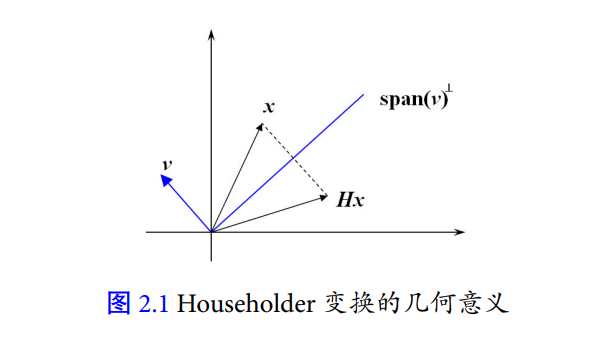
\includegraphics[scale=0.5]{figuresl/figure1.png}
\end{figure}

\noindent Householder矩阵的几个基本性质

\noindent \textcolor{blue}{定理}~设$H \in \mathbb{C}^{n \times n}$是一个 Householder 矩阵, 则
(1)$H^*=H$,即$H$ Hermite的;

(2)$H^*H=I$,即$H$是酉矩阵;

(3)$H^2=I$,所以$H^{-1}=H$;

(4)$det(H)=-1$;

(5)$H$有两个互异的特征值:$\lambda=1$和$\lambda=-1$,其中$\lambda=1$的代数重数为
$n-1$

\noindent Householder 矩阵的重要应用:
\textcolor{blue}{将一个向量除第一个元素以外的所有元素都化为零}

\noindent \textcolor{blue}{引理}~~设$x,y \in mathbb{C}^n$n 为任意两个互异的向量
, 则存在一个 Householder 矩阵$H(x)$使得$y=H(v)x$的充要条件是$\|x\|_{2}=\|y\|_{2}
\mathbb{E} x^{*} y \in \mathbb{R}$(取$v=x-y$即可)

\noindent\textcolor{blue}{定理}~设$x=\left[x_{1}, x_{2}, \ldots,
x_{n}\right]^{\top} \in \mathbb{R}^{n}$是一个非零向量, 则存在 Householder 矩阵
$H$使得$Hx=\alpha e_1$,其中$\alpha=\|x\|_2$(或$\alpha=-\|x\|_2$),$e_1=[1,0, \ldots, 0]^{\top} \in \mathbb{R}^{n}$

设$x=\left[x_{1}, x_{2}, \ldots, x_{n}\right]^{\top} \in \mathbb{R}^{n}$是一个实的非零向量, 下面讨论如何计算定理中的 Householder 矩阵$H(v)$. 由引理的证明过程可知$$
v=x-\alpha e_{1}=\left[x_{1}-\alpha, x_{2}, \ldots, x_{n}\right]^{\top}
$$

在实际计算中, 为了尽可能地减少舍入误差, 我们通常避免两个相近的数
做减法运算, 否则就会损失有效数字. 因此, 我通常取$$
\alpha=-\operatorname{sign}\left(x_{1}\right) \cdot\|x\|_{2}
$$

事实上,我们也可以取$\alpha=\operatorname{sign}\left(x_{1}\right)\|x\|_{2}$但此时为了减少舍入误差,我们需要通过下面的公式来计算$v$的第一个分量$v_1$
$$
\alpha=\operatorname{sign}\left(x_{1}\right)\|x\|_{2}
$$
$$
v_{1}=x_{1}-\alpha=\frac{x_{1}^{2}-\|x\|_{2}^{2}}{x_{1}+\alpha}=\frac{-\left(x_{2}^{2}+x_{3}^{2}+\cdots+x_{n}^{2}\right)}{x_{1}+\alpha}
$$
$$
v_{1}=\left\{\begin{array}{ll}{x_{1}-\alpha,} & {\text { if } \operatorname{sign}\left(x_{1}\right)<0} \\ {\frac{-\left(x_{2}^{2}+x_{3}^{2}+\cdots+x_{n}^{2}\right)}{x_{1}+\alpha},} & {\text { otherwise }}\end{array}\right.
$$\\无论怎样选取$\alpha$,我们都有$H=I-\beta v v^*$其中$$
\beta=\frac{2}{v^{*} v}=\frac{2}{\left(x_{1}-\alpha\right)^{2}+x_{2}^{2}+\cdots+x_{n}^{2}}=\frac{2}{2 \alpha^{2}-2 \alpha x_{1}}=-\frac{1}{\alpha v_{1}}
$$\\\textcolor {blue}{算法2.1}计算Householder向量\\\textcolor{red}{\%Given~$x \in \mathbb{R}^n$,compute~$\beta$,$v$ suth that~$Hx=\|x\|_{2} e_{1}$ with $H=I-\beta v v^*$}

\begin{enumerate}[1:]
	\item function[$\beta,v$]=house($x$)
	\item $n=$ length($x$)~(here length($x$) denotes the dimension of $x$)
	\item $\sigma=x_{2}^{2}+x_{3}^{2}+\cdots+x_{n}^{2}$
	\item $v=x$
	\item if $\sigma=0$ then
	\item        \qquad if $x_1<0$ then
	\item \qquad \qquad$v_1=2x,\beta=2/v_1^2$
	\item \qquad else
	\item \qquad \qquad $v_1=0,\beta=0$
	\item\qquad end if
	\item else
	\item \qquad $\alpha=\sqrt{x_1^2+\sigma}$ ~\% $\alpha =\|x\|_2$
	\item \qquad if $x_1<0$ then
	\item \qquad \qquad $v_1=x_1-\alpha$
	\item \qquad else
	\item \qquad \qquad $v_1=-\alpha/(x_1+\alpha)$
	\item \qquad end if 
	\item \qquad $\beta=2/(v_1^2+\alpha)$
	\item end if 
\end{enumerate}

总运算量大约为 3n, 且具有很好的数值稳定性

在实际计算时, 我们可以将向量$v$单位化,使得$v_1=1$,这样,我们就无需为$v$另外分配空间,而是将$v(2:n)$存放在$x(2:n)$中, 因为变换后的向量$x$除第一个分量外, 其它都为零.

为了避免可能产生的溢出, 可事先将$x$单位化,即令$x=x/\|x\|_2$\\

\noindent Householder 变换的运算量\\
设$A \in \mathbb{R}^{m \times n}, H=I-\beta v v^{*} \in \mathbb{R}^{m}$,则$$
H A=\left(I-\beta v v^{*}\right) A=A-\beta v v^{*} A=A-\beta v\left(A^{*} v\right)^{*}
$$

因此, 在做 Householder 变换时, 并不需要生成 Householder 矩阵, 只需要
Householder 向量即可. 上面矩阵相乘的总运算量大约为 4mn.
\subsubsection{Givens 变换}
$$G(i,j,\theta)=
\begin{bmatrix}
1& & & & & & \\
&\ddots& & & & & \\
& &c& &s& & \\
& & & \ddots& & & \\
& &-s& &c & & \\
& & & & &\ddots& \\
&&&&&&1\\
\end{bmatrix}\in \mathbb{R}^{n\times n} ~(\theta \in [0,2 \pi],i\leqslant j)
$$
Givens 变换 (或 Givens 旋转, 或 Givens 矩阵),其中$c=\cos(\theta),s=\sin (\theta)$\\

\noindent 定理:~$G(i,j,\theta)$是正交矩阵,且det$(G(i,j,\theta))=1$\\

\noindent 左乘 Givens 矩阵: 只会影响第$i$行和第$j$的元素.\\
右乘 Givens 矩阵: 只会影响第 i 和第 j 列的元素.\\

\noindent 例 ~ 设$x=\left[x_{1}, x_{2}\right]^{\top} \in \mathbb{R}^{2}$,, 则存在一个 Givens 变换$G=\left[\begin{array}{cc}{c} & {s} \\ {-s} & {c}\end{array}\right] \in \mathbb{R}^{2 \times 2}$使得$G x=[r, 0]^{\top}$,其中$c,s$和$r$的值如下:
\begin{itemize}
	\item {若$x_1=x_2=0$,则$c=1,s=0,r=0$;}
	\item{若$x_1=0$但$x_2\ne0$,则$c=0,s=x_2/\left|x_2\right|,r=\left|x_2\right|$}
	\item 若$x_1\ne 0$但$x_2=0$,则$c=$sign$(x_1),s=0,r=\left|x_1\right|$;
	\item 若$x_1\ne 0$且$x_2\ne 0$,则$c=x_1/r,s=x_2/r,r=\sqrt{x_1^2+x_2^2}$.
\end{itemize}
通过 Givens 变换, 我们可以将向量$x \in \mathbb{R}^2$的第二个分量化为 0.\\

事实上, 对于任意一个向量$x \in \mathbb{R}^n$,我们都可以通过 Givens 变换将其任意一个位置上的分量化为 0. 更进一步, 我们也可以通过若干个 Givens 变换, 将$x$中除第一个分量外的所有元素都化为 0.\\

\noindent \textcolor{blue}{算法2.2}Givens变换\\
\textcolor{red}{\%~Given~$x=[a,b]^{\top}$,compute~$c$,$s$~such that~$Gx=[r,0]^{\top}$~where~$r=\|x\|_2$}
\begin{enumerate}[1:]
	\item function~$[c,s]$ = givens$(a,b)$
	\item if $b=0$ then
	\item \qquad if $a \ge 0$then
	\item \qquad \qquad $c=1,s=0$
	\item \qquad else
	\item \qquad \qquad $c=-1,s=0$
	\item \qquad end if
	\item else
	\item \qquad if $|b|>|a|$ then
	\item \qquad \qquad $\tau=a / b, \quad s=\operatorname{sign}(b) / \sqrt{1+\tau^{2}}, \quad c=s \tau$
	\item \qquad else
	\item \qquad \qquad $\tau=b / a, \quad c=\operatorname{sign}(a) / \sqrt{1+\tau^{2}}, \quad s=c \tau$
	\item \qquad end if
	\item end if  
\end{enumerate}

\noindent \subsubsection{正交变换的舍入误差分析}
\noindent \textcolor{blue}{引理}~设$P \in \mathbb{R}^{n \times n}$是一个精确的 Householder 或 Givens 变换, $\tilde P$是其浮点运算近似, 则$$
\mathrm{fl}(\tilde{P} A)=P(A+E), \quad \mathrm{fl}(A \tilde{P})=(A+F) P
$$\\
其中$\|E\|_{2}=\mathcal{O}\left(\varepsilon_{u}\right) \cdot\|A\|_{2},\|F\|_{2}=\mathcal{O}\left(\varepsilon_{u}\right) \cdot\|A\|_{2}$\\

\noindent 这说明对一个矩阵做 Householder 变换或 Givens 变换是向后稳定的.

考虑对矩阵$A$做一系列的正交变换, 则有$$
\mathrm{fl}\left(\tilde{P}_{k} \cdots \tilde{P}_{1} A \tilde{Q}_{1} \cdots \tilde{Q}_{k}\right)=P_{k} \cdots P_{1}(A+E) Q_{1} \cdots Q_{k}
$$\\其中$\|E\|_{2}=\mathcal{O}\left(\varepsilon_{u}\right) \cdot\left(k\|A\|_{2}\right)$,这说明整个计算过程是向后稳定的\\

\noindent 一般地, 假设$X$是一个非奇异的线性变换, $\tilde{X}$是其浮点运算近似. 当$X$作用到$A$上时, 我们有$$
\mathrm{fl}(\tilde{X} A)=X A+E=X\left(A+X^{-1} E\right) \triangleq X(A+F)
$$\\
其中$\|E\|_{2}=O\left(\varepsilon_{u}\right) \cdot\|X A\|_{2} \leq O\left(\varepsilon_{u}\right) \cdot\|X\|_{2} \cdot\|A\|_{2}$,故$$
\|F\|_{2}=\left\|X^{-1} E\right\|_{2} \leq \mathcal{O}\left(\varepsilon_{u}\right) \cdot\left\|X^{-1}\right\|_{2} \cdot\|X\|_{2} \cdot\|A\|_{2}=\mathcal{O}\left(\varepsilon_{u}\right) \cdot \kappa_{2}(X) \cdot\|A\|_{2}
$$\\
因此, 舍入误差将被放大$k_2(X)$倍. 当$X$是正交变换时,$k_2(X)$达到最小
值 1, 这就是为什么在浮点运算中尽量使用正交变换的原因.\\

\subsection{QR分解}
\begin{enumerate}[3.1]
	\item \textcolor{blue}{QR分解的存在唯一性}
	\item \textcolor{blue}{基于MGS的QR分解}
	\item \textcolor{blue}{基于 Householder 变换的 QR 分解}
	\item \textcolor{blue}{列主元 QR 分解}
	\item \textcolor{blue}{基于 Givens 变换的 QR 分解}
	\item \textcolor{blue}{QR 分解的稳定性}
\end{enumerate}
\subsubsection {QR分解的存在唯一性}
\textcolor{blue}{定理(QR分解)}~设$A \in \mathbb{C}^{m \times n}(m \geq n)$.则存在一个单位列正交矩阵$Q \in \mathbb{C}^{m \times n}$和一个上三角矩阵$R \in \mathbb{C}^{n \times n}$,使得
\begin{eqnarray}
A=QR
\end{eqnarray}
\textcolor{blue}{证明}:设$A=\left[a_{1}, a_{2}, \ldots, a_{n}\right] \in \mathbb{C}^{m \times n}$\\
若$A$列满秩, 即 rank($A$) = $n$. 则 QR 分解(4)就是对$A$的列向量组进行
Gram-Schmidt 正交化过程的矩阵描述. 具体过程见下面的算法.\\
\textcolor{blue}{算法3.1}Gram-schmidt Process\\
\begin{enumerate}[1:]
	\item $r_{11}=||a_{1}||_{2}$
	\item $q_{1}=a_{1}/r_{11}$
	\item  for $j = 2$ to n do
	\item  \qquad $q_{j}=a_{j}$
	\item  \qquad for $i=1$ to $j-1$ do
	\item  \qquad \qquad $r_{ij}=q_{i}^{*}a_{j}$
	\item  \qquad \qquad $q_{j}=q_{j}-r_{ij}q_{i}$
	\item \qquad end for
	\item \qquad $r_{jj}=||q_{j}||_{2}$
	\item \qquad $q_{j}=q_{j}/r_{jj}$
	\item end for 
\end{enumerate}
如果A不是列满秩,我们可以做类似的正交化过程:
\begin{itemize}
	\item 如果$a_1=0$则令$q_1=0$;否则令$q_1=a_1/||a_1||_2$;
	\item 对于$j=2,3,\cdots$计算$\tilde{q}_{j}=a_j-\sum_{i=1}^{j-1}(q_i^*a_j)q_i$.\\
	如果$\tilde{q_j}=0$则令$q_j=0$,否则令$q_j=\tilde{q_j}/||\tilde{q_j}||_2$\\
\end{itemize}
于是我们有
\[
A=QR
\]
其中$Q=[q_1,q_2,...,q_n]$列正交(但不是单位列正交,列向量中可能有零向量).这里的$R=[r_{ij}]_{n\times n}$是上三角矩阵,定义如下
\[
r_{ij}=
\begin{cases}
q_{i}^{*} a_{j},&for i\leq j\\
0,&for i>j
\end{cases}
\]
\textcolor{blue}{易知,如果Q的某一列$q_k=0$,则R中对应的第k行全为0}\\
设$rank(A)=l<n$,则rank$(Q)=l$即Q只有$l$个非零列,不妨设为$ q_{i1},q_{i2},...q_{il} $,他们构成$ \mathbb{C}^m $的一个单位正交向量组,将其扩展成$ \mathbb{C}^m $中的一组标准正交基,即
\[
q_{i_1},q_{i_2},...q_{i_l},\tilde{q}_1,,...\tilde{q}_{m-l}
\]
然后我们用$ \tilde{q_1} $ 替换Q中的第一个零列,用$ \tilde{q}_2 $	替换Q总的第二个零列,依次类推,将Q中的所有零列都替换掉.将最后得到的矩阵记为$\tilde{Q}$,于是$\tilde{Q}\in\mathbb{C}^{m\times n}$ 单位列正交. \textcolor{blue}{由于$\tilde{Q}$中的新添加的列向量正好与$R$中的零行相对应},所以
\[
\tilde{Q}R=QR=A
\]
这就是~$A$~的~$QR$~分解\\


\noindent 满秩矩阵QR分解的存在唯一性\\

\textcolor{blue}{定理} 若A列满秩,并要求R的对角线元素都为正,则A的QR分解存在且唯一.\\

$\dagger$若A是实矩阵,则所有运算都是实运算,因此Q和R都是实矩阵.\\

$\dagger$有时也将QR分解定义为:存在酉矩阵$Q\in\mathbb{C}^{m\times m}$使得
\[
A = A\begin{bmatrix}R_{11}\\0\end{bmatrix}
\]
其中$R_{11}\in\mathbb{R}^{n\times n}$为上三角矩阵.\\

若$A$不满秩,存在置换矩阵$P$,使得$AP$的前$l$列
线性无关,其中$l=rank(A)$.对$AP$进行$QR$分解,可得:\\
\textcolor{blue}{推论} ~设$A\in\mathbb{C}^{m\times n}(m\geq n)$ 则存在一个置换矩阵$P$,使得
\[
AP=Q\begin{bmatrix}R_{11}&R_{12}\\0&0\end{bmatrix}_{n\times n}
\]
其中$Q\in\mathbb{C}^{m\times n}$单位列正交,$R_{11}\in\mathbb{C}^{l\times l}$是非奇异上三角矩阵.\\
$\dagger$上述结论可简化为
\[
AP=Q\begin{bmatrix}R_{11}&R_{12}\end{bmatrix}
\]
其中$Q\in\mathbb{C}^{m\times n}$单位列正交,$R_{11}\in\mathbb{C}^{l\times l}$是非奇异上三角矩阵.\\
\textcolor{blue}{推论(满秩分解)}~设$A\in\mathbb{C}^{m\times n}$,且$rank(A)=l\le min\{m,n\}$, 则存在满秩矩阵$F\in\mathbb{C}^{m\times l}$和$G\in\mathbb{C}^{l\times n}$ ,使得
\[
A=FG
\]

$\dagger$如果A是非奇异方阵,则QR分解可用来求解线性方程组$Ax=b$\\

$\dagger$基于G-S正交化的QR分解的运算量大约为$2mn^{2}$.\\

在后面,我们会介绍基于Householder变换的QR分解,在不需要计算Q的情况下,运算量大约为$2mn^{2}-2n^{3}/3$,如果需要计算Q,则需另外大约$2mn^{2}-2n^{3}/3$运算量.\\
\subsubsection{基于MGS的QR分解}
由于数值稳定性方面的原因,在实际计算中,我们一般不采用Gram-Schmidt过程,取而代之的是修正的是\textcolor{blue}{Gram-Schmidt过程},本算法的运算量大约为$2mn^{2}$\\
\textcolor{blue}{算法3.2}~基于MGS的QR分解\\
\textcolor{red}{\% Given $A \in \mathbb{R}^{m\times n}$, compute $Q = [q_{1},...,q_{n}]$ and R such that $A = QR$}\\
\begin{enumerate}
	\item Set $R=[r_{ik}]=0_{n\times n}$(the $n\times n$zero matrix)
	\item if $a_{1}=0$ then 
	\item \qquad $q_{1}=0$
	\item else
	\item \qquad $r_{11}=||a_{1}||_{2}$
	\item \qquad $q_{1}=a_{1}/||a_{1}||_{2}$
	\item end if
	\item for $k=2$ to n do
	\item \qquad $q_{k} = a_{k}$
	\item \qquad for $i = 1$ to $k-1$ do
	\item \qquad \qquad $r_{ik}=q_{i}^{T}q_{k}$
	\item \qquad \qquad $q_{k}=q_{k}-r_{ik}q_{i}$
	\item \qquad end for 
	\item \qquad if $q_{k}\ne 0$ then
	\item \qquad \qquad $r_{kk}=||q_{k}||_{2}$
	\item \qquad \qquad $q_{k}=q_{k}/r_{kk}$
	\item \qquad end if
	\item end for  
\end{enumerate}
$\dagger$ MGS 得到的QR分解中,$Q\in\mathbb{R}^{n\times n},R\in\mathbb{R}^{n\times n}$
\subsubsection{基于Householder变换的QR分解}
由Householder变换的性质可知,我们可以将任何一个非零变量$x\in\mathbb{R}^{n}$转化成$||x||_{2}e_{1}$,即除第一个元素外,其他都为零.\\
假定$m=n$,即$A\in\mathbb{R}^{n\times n}$ 令$H_{1}\in\mathbb{R}^{n\times n}$为Householder变换,满足
$$
H_{1}\left[\begin{array}{c}{a_{11}} \\ {a_{21}} \\ {\vdots} \\ {a_{n 1}}\end{array}\right]=\left[\begin{array}{c}{r_{1}} \\ {0} \\ {\vdots} \\ {0}\end{array}\right]
$$
于是
$$
H_{1} A=\left[\begin{array}{c|ccc}
{r_{1}}&{\tilde{a}_{12}} &\cdots& {\tilde{a}_{1 n}} \\ \hline 
0& & & \\
\vdots&&{\tilde{A}_{2}}& \\
0& & &\\
\end{array}\right],\tilde{A}_{2} \in \mathbb{R}^{(n-1) \times(n-1)}
$$
同样,构造Householder变换$\tilde{H}_{2} \in \mathbb{R}^{(n-1) \times(n-1)}$,使得
$$
\tilde{H}_{2} \tilde{A}_{2}=\left[\begin{array}{c|ccc}
{r_{1}}&{\tilde{a}_{12}} &\cdots& {\tilde{a}_{1 n}} \\ \hline 
0& & & \\
\vdots&&{\tilde{A}_{2}}& \\
0& & &\\
\end{array}\right],\tilde{A}_{2} \in \mathbb{R}^{(n-1) \times(n-1)}
$$
令$H_{2}=\left[\begin{array}{cc}{1} & {0} \\ {0} & {\tilde{H}_{2}}\end{array}\right] \in \mathbb{R}^{n \times n}$,则
$$
H_{2} H_{1} A=
\left[\begin{array}{cc|ccc}
{r_{1}} & {\tilde{a}_{12}} & {\tilde{a}_{13}} & {\cdots} &{\tilde{a}_{1 n}} \\ 
{0} & {r_{2}} & {\tilde{a}_{23}}& {\cdots} & {\tilde{a}_{2 n}} \\ 
\hline 
0 & {0} &   &  &  \\
\vdots&\vdots& &{\tilde{A}_{3}}  & \\
{0} & {0} & {} & & \end{array}\right]
$$
不断重复上述过程,这样,我们就得到一系列的矩阵
$$
H_{k}=\left[\begin{array}{cc}{I_{k-1}} & {0} \\ {0} & {\tilde{H}_{k}}\end{array}\right], \quad k=2,3, \ldots, n-1
$$
使得
$$
H_{n-1} \cdots H_{2} H_{1} A=\left[\begin{array}{cccc}{r_{1}} & {\tilde{a}_{12}} & {\cdots} & {\tilde{a}_{1 n}} \\ {0} & {r_{2}} & {\cdots} & {\tilde{a}_{2 n}} \\ {\vdots} & {} & {\ddots} & {\vdots} \\ {0} & {0} & {\cdots} & {r_{n}}\end{array}\right] \triangleq R
$$
令$Q=\left(H_{n-1} \cdots H_{2} H_{1}\right)^{-1}=H_{1} H_{2} \cdots H_{n-1}$,则
$$
A=\left(H_{n-1} \cdots H_{2} H_{1}\right)^{-1} R=Q R
$$
\textcolor{blue}{如果不需要生成Q,则运算量大约为$2mn^{2}-2/3n^{3}$}.\\

\noindent 矩阵$Q$的计算\\
可通过下面的算法实现
$$
Q=I_{n}, \quad Q=Q H_{k}, \quad k=1,2, \ldots, n-1
$$
若保留了所有的Householder向量,则Q可以通过下面的\textcolor{blue}{向后累积法}实现:
$$
Q=I_{n}, \quad Q=H_{k} Q, \quad k=n-1, n-2, \ldots, 1
$$
\textcolor{blue}{优点:一开始Q会比较稀疏,随着迭代的进行,Q才会慢慢变满}\\
运算量大约为$4(m^{2}n-mn^{2}+\frac{1}{3}n^{3})$.\\
$\dagger$若$m>n$ 则由Householder变换得到的QR分解中,$Q\in\mathbb{R}^{m\times m},R\in\mathbb{R}^{m\times n}$
\textcolor{blue}\\

\noindent \textcolor{blue}{算法3.3}基于Householder变换的QR分解\\
\textcolor{red}{\%Given$A \in \mathbb{R}^{m×\times n}$,compute$Q \in \mathbb{R}^{m\times m}$,$R\in \mathbb{R}^{m\times n}$ such that $A = QR$ \% The upper triangular part of R is stored in the upper triangular part of A}
\begin{enumerate}[1:]
	\item Set $Q=I_{m\times m}$
	\item for $k=1$ to n do
	\item \qquad $x=A(k:m,k)$
	\item \qquad$[\beta, v_{k}]$ = house(x)
	\item \qquad$v_{k} = v_{k}||v||2$
	\item \qquad$A(k:m,k:n)=(I_{m-k+1} −2v_{k}v_{k}^{T})A(k:m,k:n)$
	\item \qquad$Q(1:k−1,k:m)=Q(1:k−1,k:m)(I_{m−k+1} -2v_{k}v_{k}^{⊺})$
	\item \qquad$Q(k:m,k:m)=Q(k:m,k:m)(I_{m−k+1} -2v_{k}v_{k}^{T})$
	\item end for
\end{enumerate}
\textcolor{blue}{上面的算法只是一个简单描述, 并没有考虑运算量问题}.\\

$\dagger$在实际计算时, 我们通常会保留所有的 Householder 向量.\\

由于第k步中$\hat{H}_{k}$ 所对应的Householder向量$v_{k}$ 的长度为$m−k+1$, 因此我们先把 $v_{k}$ 单位化, 使得 $v_{k}$ 的第一元素为 1, 这样就只要存储 $v_{k}(2:end)$, 共 $m - k$ 个元素.\\

\textcolor{blue}{这样, 我们就可以把所有的 Householder 向量存放在 A 的严格下三 角部分, 而 A 的上三角部分仍然存放 R.}\\

在计算 Q 时采用向后累积的方法, 所以总的运算量大约为 $4m^{2}n - 2mn^{2} + 2n^{3}$. 若 $m = n$, 则运算量大约为 $8n^{3}$.\\

$\dagger$我们也可以考虑分块 Householder QR 分解, 以便充分利用 3 级 BLAS 运算, 提高计算效率.\\
\subsubsection{列主元QR分解}
\noindent 当 A 不是满秩时, 我们可以进行\textcolor{blue}{列主元 QR 分解.}\\
\textcolor{blue}{定理(列主元QR分解)}~设$A \in \mathbb{C}^{m \times n}(m \geq n)$,且$\operatorname{rank}(A)=k<n$,则存在置换矩阵 P, 正交矩阵$Q \in \mathbb{C}^{m \times m}$,使得
$$
A P=Q\left[\begin{array}{cc}{R_{11}} & {R_{12}} \\ {0} & {0}\end{array}\right]_{m \times n}
$$
其中$R_{11} \in \mathbb{C}^{k \times k}$是非奇异上三角矩阵,且对角线元素满足$r_{11} \geq r_{22} \geq \cdots \geq r_{k k}>0$\\

列主元 QR 分解的实现过程与 QR 分解基本类似, 只是每一步需要选个列 主元, 同时做一个列交换\\

假设经过$l$步后,我们得到下面的分解
$$
A P^{(l)}=Q^{(l)}\left[\begin{array}{cc}{R_{11}^{(l)}} & {R_{12}^{(l)}} \\ {0} & {R_{22}^{(l)}}\end{array}\right] \triangleq Q^{(l)} R^{(l)},或 \left(Q^{(l)}\right)^{\top} A P^{(l)}=R^{(l)}
$$
其中$P^(l)$为置换矩阵,$Q^(l)$为正交矩阵,$R_{12}^{(l)} \in \mathbb{R}^{(l) \times(l)}$非奇异上三角矩阵.\\
下面进行第$l+1$步:
\begin{enumerate}
	\item 计算 $R_{22}^{(l)}$ 所有列的范数, 若都为 0, 则算法结束, 此时必有 $l = k$.
	\item 若$l < k$,则$R_{22}^{(l)}\ne 0$. 设范数最大的列为第$i_{l+1}$列(若有相等的,取其中一列即可), 范数为 $r_{l+1,l+1}$. 若 $i_{l+1}\ne 1$, 则交换 $R(l)$ 的第 $l + 1$ 列与第 $i_{l+1} + l$ 列, 并记相应的置换矩阵为 $P_{l+1}$.
	\item 以 $R_{22}^{(l)}$ 的第 1 列构造 Householder 变换 $\bar{H}_{l+1}$\\
	令$H_{l+1}=Blkdiag(I_{l},\bar{H}_{l+1}),P^{(l+1)}=P^{(l)} P_{l+1}$.则
\end{enumerate}
$$
H_{l+1}\left(Q^{(l)}\right)^{\top} A P^{(l+1)}=H_{l+1} R^{(l)} P_{l+1}=\left[\begin{array}{cc}{R_{11}^{(l)}} & {\tilde{R}_{12}^{(l)}} \\ {0} & {\tilde{R}_{22}^{(l)}}\end{array}\right] \triangleq R^{(l+1)}
$$
其中 $\tilde {R}_{22}^{(l)}$ 的第一列除第一个元素外, 其余都是零, 且该元素等于$r_{l+1,l+1}$,即
$$
R^{(l+1)}=\left[\begin{array}{c c |c c}{R_{11}^{(l)}} & {*} & {*} \\ {0} & {r_{l+1, l+1}} & {*} \\ \hline {0} & {0} & {*}\end{array}\right] \triangleq\left[\begin{array}{cc}{R_{11}^{(l+1)}} & {R_{12}^{(l+1)}} \\ {0} & {R_{22}^{(l+1)}}\end{array}\right]
$$
其中$R_{11}^{(l+1)} \in \mathbb{R}^{(l+1) \times(l+1)}$为非奇异上三角矩阵\\
记$Q^{(l+1)} \triangleq Q^{(l)} H_{l+1}^{\top}$,则
$$
A P^{(l+1)}=Q^{(l+1)} R^{(l+1)}
$$
依此类推, 直到第 k 步, 即可得 A 的列主元 QR 分解.\\
矩阵 R11 的对角线元素的递减关系可由列主元的选取方法推出.
\subsubsection{基于Givens变换的QR分解}
我们同样可以利用 Givens 变换来做 QR 分解.\\
设$A \in \mathbb{R}^{n \times n}$,构造 Givens 变换 $G_{21}$, 作用在 A 的最前面的两行上, 使得
$$
G_{21}\left[\begin{array}{c}{a_{11}} \\ {a_{21}} \\ {a_{31}} \\ {\vdots} \\ {a_{n 1}}\end{array}\right]=\left[\begin{array}{c}{\tilde{a}_{11}} \\ {0} \\ {a_{31}} \\ {\vdots} \\ {a_{n 1}}\end{array}\right]
$$
构造Givens变换$G_{31}$,作用在$G_{21}A$的第1行和第3行上,将$a_{31}$ 化为零. 由于 $G_{31}$ 只改变第 1 行和第 3 行的值, 所以第二行的零元素维持不变.以此类推, 我们可以构造一系列的 Givens 变换 $G_{41}, G_{51}, \ldots, G_{n 1}$ 使得 $G_{n 1} \cdots G_{21} A$ 的第一列中除第一个元素外, 其它元素都化为零, 即
$$
G_{n 1} \cdots G_{21} A=
\left[\begin{array}{cccc}
{*} & {*} & {\cdots} & {*} \\ 
{0} & {*} & {\cdots} & {*} \\ 
{\vdots} & {\vdots} & & {\vdots} \\ 
{0} & {*} & {\cdots} & {*}
\end{array}\right]
$$
下面我们可以对第二列进行类似的处理. 构造 Givens 变换 $G_{32}, G_{42}, \ldots, G_{n 2}$将第二列的第 3 至第 n 个元素全化为零, 同时保持第一列不变. \\
其他列也做类似的处理. 最后, 通过构造$\frac{1}{2} n(n-1)$个 Givens 变换, 将转化成一个上三角矩阵$R$, 即
$$
R=G_{n, n-1} \cdots G_{21} A,或A=\left(G_{n, n-1} \cdots G_{21}\right)^{\top} R \triangleq Q R
$$
$\dagger$与 Householder 变换一样, 在进行 Givens 变换时, 我们不需要显式地 写出 Givens 矩阵.\\
$\dagger$对于稠密矩阵而言, 基于 Givens 变换的 QR 分解的运算量比 House- holder 变换要多很多.\\
\textcolor{blue}{基于 Givens 变换的 QR 分解主要用于当矩阵的非零下三角元素相对 较少时的情形, 比如对上 Hessenberg 矩阵进行 QR 分解}\\
$\dagger$如果 $A \in \mathbb{R}^{m\times n}, m > n$, 仍然可以通过 Givens 变换进行 QR 分解\\

\textcolor{blue}{算法3.4:}基于 Givens 变换的 QR 分解\\
\textcolor{red}{\%Given $A \in \mathbb{R}^{m\times n}$,compute$Q \in \mathbb{R}^{m×\times m}$ and$R\in \mathbb{R}{m\times n}$ such that $A = QR$\\
	\% The upper triangular part of R is stored in the upper triangular part of A}
\begin{enumerate}[1:]
	\item Set $Q=I_{m\times m}$
	\item for $k=1$ to n do
	\item \qquad for i = k + 1 to m do
	\item \qquad \qquad $[c, s]=givens(a_{kk}, a_{ik})$
	\item \qquad \qquad $\left[\begin{array}{c}{A(k, k : n)} \\ {A(i, k : n)}\end{array}\right]=G\left[\begin{array}{c}{A(k, k : n)} \\ {A(i, k : n)}\end{array}\right]$ where $G=\left[\begin{array}{cc}{c} & {s} \\ {-s} & {c}\end{array}\right]$
	\item \qquad \qquad $[Q(1 : m, k), Q(1 : m, i)]=[Q(1 : m, k), Q(1 : m, i)] G^{\top}$
	\item \qquad end for
	\item end for
\end{enumerate}
\subsubsection{QR分解的稳定性}
\noindent 基于 Householder 变换和 Givens 变换的 QR 分解都具有很好的数值稳定性, 基于 MGS 的 QR 分解也是向后稳定的\\
$\dagger$如果需要计算 Q, 则 MGS 的运算量相对较少, 因此当 A 的列向量具有很好的线性无关性时, 我们可以使用 MGS 来计算 QR 分解.\\
Björck [Björck 1967] 证明了, 通过 MGS 计算的矩阵 Q 满足
$$
Q^{\top} Q=I+E_{M G S},~~\left\|E_{M G S}\right\|_{2} \approx \varepsilon_{u} \kappa_{2}(A)
$$
而 Householder 变换计算的矩阵 Q 满足
$$
Q^{\top} Q=I+E_{H},~~\left\|E_{H}\right\|_{2} \approx \varepsilon_{u}
$$
因此, 如果正交性至关重要, 建议使用 Householder 变换, 特别是当 A 的列 向量接近线性相关时
\subsection{奇异值分解}
\textcolor{blue}{定理(SVD)}设$A \in \mathbb{C}^{m \times n}(m \geq n)$则存在酉矩阵$U \in \mathbb{C}^{m \times m}$和$V \in \mathbb{C}^{n \times n}$,使得
\begin{equation}
U^{*} A V=\left[\begin{array}{l}{\Sigma} \\ {0}\end{array}\right],orA=U\left[\begin{array}{l}{\Sigma} \\ {0}\end{array}\right] V^{*}
\end {equation}
其中$\Sigma=\operatorname{diag}\left(\sigma_{1}, \sigma_{2}, \ldots, \sigma_{n}\right) \in \mathbb{R}^{n \times n}$,且$\sigma_{1} \geq \ldots \geq \sigma_{n} \geq 0$\\

$\dagger$该定理也可以通过 Hermite 半正定矩阵的特征值分解来证明.\\

\textcolor{blue}{定义} 分解(3.6)称为$A$的\textcolor{blue}{奇异值分解(SVD)},$\sigma_{1}, \sigma_{2}, \dots, \sigma_{n}$称为A的奇 异值, 它们是矩阵 $A^{*}A$ 的特征值的平方根.\\

$\dagger$在不做特别说明的情况下,我们总是假定$\sigma_{1} \geq \sigma_{2} \geq \cdots \geq \sigma_{n} \geq 0$\\
$\dagger$如果$A \in \mathbb{R}^{m \times n}$是实矩阵, 则 U , V 也都可以是实矩阵 [Horn-Johnson1985].\\

\noindent 奇异向量\\
矩阵$U=\left[u_{1}, u_{2}, \ldots, u_{m}\right]$和$V=\left[v_{1}, v_{2}, \ldots, v_{n}\right]$的列向量分别称为 A 的\textcolor{blue}{左奇异向量}和\textcolor{blue}{右奇异向量}, 即存在关系式
$$
\begin{array}{l}{A v_{i}=\sigma_{i} u_{i}, \quad i=1,2, \ldots, n} \\ {A^{*} u_{i}=\sigma_{i} v_{i}, \quad i=1,2, \ldots, n} \\ {A^{*} u_{i}=0, \quad i=n+1, n+2, \ldots, m}\end{array}
$$
SVD的其他形式\\
$$
A=U\left[\begin{array}{l}{\Sigma} \\ {0}\end{array}\right] V^{*}=\sigma_{1} u_{1} v_{1}^{*}+\sigma_{2} u_{2} v_{2}^{*}+\cdots+\sigma_{n} u_{n} v_{n}^{*}
$$
记$U_{n}=\left[u_{1}, u_{2}, \ldots, u_{n}\right] \in \mathbb{C}^{m \times n}$,则$U_{n}$是单位列正交矩阵,且
\begin{equation}
A=U_{n} \Sigma V^{*}
\end{equation}
这就是所谓的细 SVD (thin SVD ) 或 降阶 SVD (reduced SVD ), 有的文献 将上式称为奇异值分解.\\
当$k < n$时,我们称
$$
A_{k}=\sigma_{1} u_{1} v_{1}^{*}+\sigma_{2} u_{2} v_{2}^{*}+\cdots+\sigma_{k} u_{k} v_{k}^{*}
$$
为 A 的截断 SVD (truncated SVD ).\\

\noindent 奇异值分解基本性质\\
\textcolor{blue}{定理:}设$A=U\left[\begin{array}{l}{\Sigma} \\ {0}\end{array}\right] V^{*}$是$A \in \mathbb{C}^{m \times n}(m \geq n)$的奇异值分解,则
\begin{enumerate}[(1)]
	\item $A^{*} A$ 的特征值是 $\sigma_{i}^{2}$ , 对应的特征向量是 $v_{i}$
	\item $AA^{*}$的特征值是$\sigma_{i}^{2}$和$m-n$个零,对应的特征向量是$u_{i}$
	\item $\|A\|_{2}=\sigma_{1},\|A\|_{F}=\sqrt{\sigma_{1}^{2}+\sigma_{2}^{2}+\cdots+\sigma_{n}^{2}}$
	\item 若$\operatorname{rank}(A)=r \leq n$,则$\operatorname{Ran}(A)=\operatorname{span}\left\{u_{1}, u_{2}, \ldots, u_{r}\right\}$,$\operatorname{Ker}(A)=\operatorname{span}\left\{v_{r+1}, v_{r+2}, \ldots, v_{n}\right\}$
	\item 设$x \in \mathbb{C}^{n}$,且$\|x\|_{2}=1$和$Y \in \mathbb{C}^{n \times n}$是酉矩阵,则$\sigma_{i}\left(X^{*} A Y\right)=\sigma_{i}(A)$
	\item (酉不变性)$X \in \mathbb{C}^{m \times m}$和$Y \in \mathbb{C}^{n \times n}$是酉矩阵,则$\sigma_{i}\left(X^{*} A Y\right)=\sigma_{i}(A)$
\end{enumerate}
\textcolor{blue}{定理} 设$A=U \Sigma V^{*}$是$A \in \mathbb{C}^{n \times n}$的奇异值分解,则:
\begin{enumerate}[(1)]
	\item $|\operatorname{det}(A)|=\sigma_{1} \sigma_{2} \cdots \sigma_{n}$
	\item 若A非奇异,则$\left\|A^{-1}\right\|_{2}=\sigma_{n}^{-1}, \kappa_{2}(A)=\sigma_{1} / \sigma_{n}$
	\item 若A是Hermite的,且$A=U \Lambda U^{*}$是A的酉特征值分解,设$\left|\lambda_{1}\right| \geq\left|\lambda_{2}\right| \geq \cdots \geq\left|\lambda_{n}\right|$,则$A=U \Sigma V$是A的奇异值分解,其中$\sigma_{i}=\left|\lambda_{i}\right|, v_{i}=\operatorname{sign}\left(\lambda_{i}\right) u_{i}$,若$\lambda_{i}=0$,则$v_{i}=u_{i}$
	\item 矩阵$\left[\begin{array}{cc}{0} & {A^{*}} \\ {A} & {0}\end{array}\right]$的特征值是$\pm \sigma_{i}$,对应单位特征向量$\frac{1}{\sqrt{2}}\left[\begin{array}{c}{v_{i}} \\ { \pm u_{i}}\end{array}\right]$
\end{enumerate}
$\dagger$矩阵条件数取决于奇异值, 不是特征值, 见讲义上的例子\\

低秩逼近\\

\textcolor{blue}{定理}设$A=U_{n} \Sigma V^{*}$是$A \in \mathbb{C}^{m \times n}$的奇异值分解. 令
$$
A_{k}=\sum_{i=1}^{k} \sigma_{i} u_{i} v_{i}^{*}
$$
则$A_{k}$是
\begin{equation}
\min _{B \in \mathbb{C}^{m \times n}, \operatorname{rank}(B)=k}\|A-B\|_{2}
\end{equation}
的一个解, 且
$$
\left\|A-A_{k}\right\|_{2}=\sigma_{k+1}
$$
此时,我们称Ak 是A的一个\textcolor{blue}{秩k逼近}\\
$\dagger$对于 Frobenius 范数, 我们有类似的结论.\\

\textcolor{blue}{定理(Weyl)}设$A, B \in \mathbb{C}^{m \times n}(m \geq n)$且$\operatorname{rank}(B)=k$,则有
\begin{equation}
\max _{x \in \operatorname{Ker}(B),\|x\|_{2}=1}\|A x\|_{2} \geq \sigma_{k+1}(A)
\end{equation}
和
\begin{equation}
\min _{x \in \operatorname{Ker}(B),\|x\|_{2}=1}\|A x\|_{2} \leq \sigma_{n-k}(A)
\end{equation}
因此,
\begin{equation}
\sigma_{1}(A-B) \geq \sigma_{k+1}(A), \quad \sigma_{n}(A+B) \leq \sigma_{n-k}(A)
\end{equation}
且
\begin{equation}
\sigma_{i+j-1}(A) \leq \sigma_{i}(B)+\sigma_{j}(A-B), \quad i=1,2, \ldots, n, j=1,2, \ldots, n-i+1
\end{equation}
根据 Weyl 定理, 我们可以得到矩阵奇异值的最小最大定理.\\

\textcolor{blue}{定理}设$\sigma_{1} \geq \sigma_{2} \geq \cdots \geq \sigma_{n} \geq 0$是矩阵$A \in \mathbb{C}^{m \times n}(m \geq n)$的奇异值,则
$$
\sigma_{k}(A)=\min _{\operatorname{dim}(\mathcal{L})=n-k+1} \max _{x \in \mathcal{L},\|x\|_{2}=1}\|A x\|_{2}, \quad k=1,2, \ldots, n
$$
和
$$
\sigma_{k}(A)=\max _{\operatorname{dim}(\mathcal{L})=k} \min _{x \in \mathcal{L},\|x\|_{2}=1}\|A x\|_{2}, \quad k=1,2, \ldots, n
$$
其中$\mathcal{L}$表示$\mathbb{C}^{n}$ 的一个子空间.\\

\textcolor{blue}{引理(交错不等式)}设$A \in \mathbb{C}^{m \times n}, A_{r}$是由A去除r列(或r行)后得到的子矩阵,则
$$
\sigma_{i}(A) \geq \sigma_{i}\left(A_{r}\right) \geq \sigma_{i+r}(A), \quad i=1,2, \ldots, \min \{m, n\}
$$
这里, 当下标 k 大于矩阵的维数时, 我们令 $\sigma_{k} = 0$.
更进一步, 如果$B \in \mathbb{C}^{(m-r) \times(n-s)}$是A的子矩阵,则
$$
\sigma_{i}(A) \geq \sigma_{i}(B) \geq \sigma_{i+r+s}(A)
$$
\textcolor{blue}{引理}设$A \in \mathbb{C}^{n \times n}, 1 \leq k \leq n$则对任意的单位列正交矩阵$U_{k} \in \mathbb{C}^{n \times k}$和$V_{k} \in \mathbb{C}^{n \times k}$,有
\begin{equation}
\sigma_{i}\left(U_{k}^{*} A V_{k}\right) \leq \sigma_{i}(A), \quad i=1,2, \ldots, k
\end{equation}
因此,
\begin{equation}
\left|\operatorname{det}\left(U_{k}^{*} A V_{k}\right)\right| \leq \sigma_{1}(A) \sigma_{2}(A) \cdots \sigma_{k}(A)
\end{equation}
\textcolor{blue}{定理(Weyl不等式,1949)}设$A \in \mathbb{C}^{n \times n}$其奇异值和特征值分别为$\sigma_{1} \geq \sigma_{2} \geq \cdots \geq \sigma_{n} \geq 0$和$\left|\lambda_{1}\right| \geq\left|\lambda_{2}\right| \geq \cdots \geq\left|\lambda_{n}\right|$则
$$
\left|\lambda_{1} \lambda_{2} \cdots \lambda_{k}\right| \leq \sigma_{1} \sigma_{2} \cdots \sigma_{k}, \quad k=1,2, \ldots, n
$$
且当 $k = n$ 时, 等号成立.\\

奇异值扰动分析\\

\textcolor{blue}{定理}~设$A, E \in \mathbb{C}^{m \times n}(m \geq n)$,则
$$
\left|\sigma_{i}(A+E)-\sigma_{i}(A)\right| \leq\|E\|_{2}, \quad i=1,2, \ldots, n
$$
下面是上述定理的一个推论, 也是 SVD 的一个重要应用\\

\textcolor{blue}{推论}~设$A \in \mathbb{C}^{n \times n},\|\cdot\|$是任一相容矩阵范数,则对任意的$\varepsilon>0$
总存在矩阵$A_{\varepsilon}$,使得$\left\|A-A_{\varepsilon}\right\| \leq \varepsilon$,其中$A_{\varepsilon}$具有互不相同的特征值.\\
因此, \textcolor{blue}{可对角化矩阵在所有矩阵组成的集合中是稠密的}
\subsection{线性最小二乘问题的求解方法}
\begin{enumerate}[5.1]
	\item 正规方程法
	\item QR分解法
	\item 奇异值分解法
\end{enumerate}
\subsubsection{正规方程法}
\textcolor{blue}{定理} 设$A \in \mathbb{R}^{m \times n}(m \geq n)$,则$x_{*} \in \mathbb{R}^{n}$是线性最小二乘问题的解当且仅当残量$r=b-A x_{*}$与$\operatorname{Ran}(A)$正交,即$x_{*}$是下面的\textcolor{blue}{正规方程}的解
\begin{equation}
A^{\top}(b-A x)=0 \quad \text { 或 } \quad A^{\top} A x=A^{\top} b
\end{equation}
由于
$$
A^{\top} b \in \operatorname{Ran}\left(A^{\top}\right)=\operatorname{Ran}\left(A^{\top} A\right)
$$
因此正规方程$A^{\top} A x=A^{\top} b$总是相容的,即\textcolor{blue}{最小二乘解总是存在的},且当 A 满秩时, 这个解也是唯一的.\\

\textcolor{blue}{定理} 设$A \in \mathbb{R}^{m \times n}(m>n)$,则$A^{\top} A$对称正定当且仅当$A$是列满秩的,即
$\operatorname{rank}(A)=n$,此时,线性最小二乘问题的解是唯一的,其表达式为
$$
x=\left(A^{\top} A\right)^{-1} A^{\top} b
$$
当 A 列满秩时, 我们就可以使用 Cholesky 分解来求解正规方程, 总的运算量大约为$mn^{2}+1/3n^{3}+\mathbb{O}(n^{2})$,其中大部分的运算量($mn^{2}$)是用来计算$A^{T}A$(由于$A^{T}A$对称,因此只需计算其下三角部分).\\

\textbf{最小二乘的几何含义}\\
我们可以把$b$写成
\begin{equation}
b=A x_{*}+r, \text  {其中} r \perp \operatorname{Ran}(A)
\end{equation}
所以 $Ax_{*}$ 就是$b$在 $Ran(A)$ 上的正交投影:
\begin{figure}[htbp]
	\begin{center}
		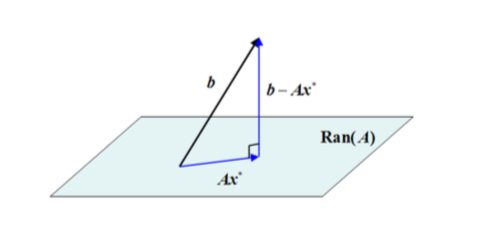
\includegraphics[scale=1]{figuresl/figure2.png}
		\label{default}
	\end{center}
\end{figure}
\\
$\dagger$最小二乘解可能并不唯一, 但b的上述分解总是唯一的.\\

最小二乘与鞍点问题\\
线性最小二乘问题 (3.1) 等价于
$$
A^{\top} r=0, \quad r=b-A x
$$
即
\begin{equation}
\left[\begin{array}{cc}{I} & {A} \\ {A^{\top}} & {0}\end{array}\right]\left[\begin{array}{l}{r} \\ {x}\end{array}\right]=\left[\begin{array}{l}{b} \\ {0}\end{array}\right]
\end{equation}
这就是线性最小二乘问题 (3.1) 的\textcolor{blue}{增广方程} (augmented system). 事实上,
方程组 (16) 是下面方程组的一种特殊情形
$$
\left[\begin{array}{cc}{B} & {A} \\ {A^{\top}} & {0}\end{array}\right]\left[\begin{array}{l}{r} \\ {x}\end{array}\right]=\left[\begin{array}{l}{f} \\ {g}\end{array}\right]
$$
其中$B \in \mathbb{R}^{m \times m}$ ~对称半正定. 这就是通常所说的鞍点问题. 这个方程组 存在唯一解当且仅当 A 列满秩且矩阵 [B, A] 行满秩.\\
如果 B 对称正定, 则$r=B^{-1}(f-A x)$,代入第二个方程可得
$$
A^{\top} B^{-1} A x=A^{\top} B^{-1} f-g
$$
这就是\textcolor{blue}{广义的正规方程}. 其所对应的\textcolor{blue}{广义线性最小二乘问题}是
$$
\min _{x \in \mathbb{R}^{n}} \frac{1}{2}\|A x-f\|_{B^{-1}}^{2}+g^{\top} x
$$
其中范数$\|\cdot\|_{B^{-1}}$的定义是$\|x\|_{B^{-1}}^{2}=x^{\top} B^{-1} x$.
\subsubsection{QR分解法}
假定$A \in \mathbb{R}^{m \times n}(m \geq n)$满秩,用三种不同方法来推导
\begin{enumerate}[(1)]
	\item 将 Q 的扩充成一个正交矩阵, 记为$[Q, \hat{Q}] \in \mathbb{R}^{m \times m}$于是有
	$$
	\begin{aligned}\|A x-b\|_{2}^{2} &=\left\|[Q, \hat{Q}]^{\top}(A x-b)\right\|_{2}^{2} \\ &=\left\|[Q, \hat{Q}]^{\top}(Q R x-b)\right\|_{2}^{2} \\ &=\left\|\left[\begin{array}{c}{R x-Q^{\top} b} \\ {-\hat{Q}^{\top} b}\end{array}\right]\right\|_{2}^{2} \\ &=\left\|R x-Q^{\top} b\right\|_{2}^{2}+\left\|\hat{Q}^{\top} b\right\|_{2}^{2} \geq\left\|\hat{Q}^{\top} b\right\|_{2}^{2} \end{aligned}
	$$等号成立当且仅当 $R x=Q^{\top} b$所以最小二乘解为
	$$
	x_{*}=R^{-1} Q^{\top} b
	$$
	\item 将b写成$b=\left(Q Q^{\top}+I-Q Q^{\top}\right) b$,则
	$$
	\begin{aligned} A x-b &=A x-\left(Q Q^{\top}+I-Q Q^{\top}\right) b \\ &=\left(A x-Q Q^{\top} b\right)-\left(I-Q Q^{\top}\right) b \end{aligned}
	$$
	由于$QQ^{T}$是$Ran(A)$上的正交投影,因此$A x-Q Q^{\top} b$与$\left(I-Q Q^{\top}\right) b$正交. 所以
	$$
	\begin{aligned}\|A x-b\|_{2}^{2} &=\left\|A x-Q Q^{\top} b\right\|_{2}^{2}+\left\|\left(I-Q Q^{\top}\right) b\right\|_{2}^{2} \\ &=\left\|R x-Q^{\top} b\right\|_{2}^{2}+\left\|\left(I-Q Q^{\top}\right) b\right\|_{2}^{2} \\ & \geq\left\|\left(I-Q Q^{\top}\right) b\right\|_{2}^{2} \end{aligned}
	$$等号成立当且仅当$R x=Q^{\top} b$ 所以最小二乘解为
	$$
	x_{*}=R^{-1} Q^{\top} b
	$$
	\item 解正规方程. 由定理 5.1 可知, 最小二乘解为
	$$
	\begin{aligned} x_{*} &=\left(A^{\top} A\right)^{-1} A^{\top} b \\ &=\left(R^{\top} Q^{\top} Q R\right)^{-1} R^{\top} Q^{\top} b \\ &=\left(R^{\top} R\right)^{-1} R^{\top} Q^{\top} b \\ &=R^{-1} Q^{\top} b \end{aligned}
	$$
\end{enumerate}
$\dagger$用 QR 分解来求最小二乘解的运算量大约为 $2mn^{2}$ (如果采用 Householder 变换的话, 运算量大约为 $2mn^{2} - 2/3n^{3}$). 当 $m \gg n$ 时, 大约为正规方程的两倍. 当 $m = n$ 时, 几乎相同.\\
$\dagger$通常 QR 算法比较稳定, 是求解最小二乘问题的首选方法, 特别是当 A 条件数较大 (病态) 时.
\subsubsection{奇异值分解法}
设$A \in \mathbb{R}^{m \times n}$列满秩,$A=U\left[\begin{array}{l}{\Sigma} \\ {0}\end{array}\right] V^{\top}$是A的奇异值分解,$U=\left[U_{n}, \tilde{U}\right]$
则
$$
\begin{aligned}\|A x-b\|_{2}^{2}=\left\|U\left[\begin{array}{c}{\Sigma} \\ {0}\end{array}\right] V^{\top} x-b\right\|_{2}^{2} &=\left\|\left[\begin{array}{c}{\Sigma} \\ {0}\end{array}\right] V^{\top} x-\left[U_{n}, \tilde{U}\right]^{\top} b\right\|_{2}^{2} \\ &=\left\|\left[\begin{array}{c}{\Sigma V^{\top} x-U_{n}^{\top} b} \\ {-\tilde{U}^{\top} b}\end{array}\right]\right\|_{2}^{2} \\ &=\left\|\Sigma V^{\top} x-U_{n}^{\top} b\right\|_{2}^{2}+\left\|\tilde{U}^{\top} b\right\|_{2}^{2} \geq\left\|\tilde{U}^{\top} b\right\|_{2}^{2} \end{aligned}
$$
等号当且仅当$\Sigma V^{\top} x-U_{n}^{\top} b=0$时成立, 即
$$
x=\left(\Sigma V^{\top}\right)^{-1} U_{n}^{\top} b=V \Sigma^{-1} U_{n}^{\top} b
$$
这就是线性最小二乘问题 (3.1) 的解.
\subsection{广义逆与最小二乘}

\subsubsection{广义逆的定义}
\noindent 广义逆的概念最早由 Moore 于 1920 年提出:\\

设$A \in \mathbb{C}^{m \times n}$,若$X \in \mathbb{C}^{n \times m}$满足
\begin{equation}
A X=P_{\operatorname{Ran}(A)}, \quad X A=P_{\operatorname{Ran}(X)}
\end{equation}
即$AX$和$XA$分别为Ran($A$)和Ran($X$)上的正交投影,则称$X$是$A$的
广义逆.\\

1955 年, Penrose 利用四个矩阵方程给出了广义逆的定义.\\

\textcolor{blue}{定义}~设$A \in \mathbb{C}^{m \times n}$,若$X \in \mathbb{C}^{n \times m}$满足
\begin{equation}
AXA=A 
\end{equation} 
\begin{equation}
XAX=X
\end{equation}
\begin{equation}
(AX)^*=AX
\end{equation}
\begin{equation}
(X A)^{*}=X A 
\end{equation}
则称 X 为 A 的\textcolor{blue}{广义逆} (或 \textcolor{blue}{Moore-Penrose 逆}, 简称 \textcolor{blue}{MP 逆}), 记为 $A\dagger$\\

$\dagger$可以证明, 以上两个定义是等价的.\\

$\dagger$若$A \in \mathbb{C}^{m \times n}$非奇异,则$A^{\dagger}=A^{-1}$\\

\textcolor{blue}{定义}~设$A \in \mathbb{C}^{m \times n}$则满足矩阵方程 (18)-(21) 的矩阵$X \in \mathbb{C}^{n \times m}$存在唯一,即广义逆存在且惟一.\\

广义逆与SVD\\
设$A \in \mathbb{C}^{m \times n}\operatorname{rank}(A)=r>0, A$的SVD为
$$
A=U\left[\begin{array}{cc}{\Sigma_{1}} & {0} \\ {0} & {0}\end{array}\right] V^{*}, \quad \Sigma_{1}=\operatorname{diag}\left(\sigma_{1}, \sigma_{2}, \ldots, \sigma_{r}\right) \in \mathbb{R}^{r \times r}
$$
则容易验证
$$
A^{\dagger}=V\left[\begin{array}{cc}{\Sigma_{1}^{-1}} & {0} \\ {0} & {0}\end{array}\right] U^{*}
$$
\subsection{广义逆的基本性质}
\noindent \textcolor{blue}{定理}~设$A \in \mathbb{C}^{m \times n}$,则\begin{enumerate}[(1)]
	\item $(A^{\dagger})^{\dagger}=A$
	\item $(A^{T})^{\dagger}=(A^{\dagger})^{T},(A^{*})^{\dagger}=(A^{\dagger})^{*}$
	\item $\operatorname{rank}(A)=\operatorname{rank}\left(A^{\dagger}\right)=\operatorname{rank}\left(A^{\dagger} A\right)$
	\item $\left(A A^{*}\right)^{\dagger}=\left(A^{*}\right)^{\dagger} A^{\dagger},\left(A^{*} A\right)^{\dagger}=A^{\dagger}\left(A^{*}\right)^{\dagger}$
	\item $\left(A A^{*}\right)^{\dagger} A A^{*}=A A^{\dagger},\left(A^{*} A\right)^{\dagger} A^{*} A=A^{\dagger} A$
	\item $A^{\dagger}=\left(A^{*} A\right)^{\dagger} A^{*}=A^{*}\left(A A^{*}\right)^{\dagger}$特别地, 若 A 列满秩, 则$A^{\dagger}=\left(A^{*} A\right)^{-1} A^{*}$.若A行满秩,则$A^{\dagger}=A^{*}\left(A A^{*}\right)^{-1}$
	\item 若U,V是酉矩阵,则$(U A V)^{\dagger}=V^{*} A^{\dagger} U^{*}$
\end{enumerate}
$\dagger$一般来说,当A,B是方阵时,
\begin{itemize}
	\item $(A B)^{\dagger} \neq B^{\dagger} A^{\dagger}$
	\item $A A^{\dagger} \neq A^{\dagger} A$
	\item $\left(A^{k}\right)^{\dagger} \neq\left(A^{\dagger}\right)^{k}$
	\item A和$A^{\dagger}$的非零特征值并不是互为倒数
\end{itemize}
设~$A \in \mathbb{C}^{m \times n}$,则
$$
\begin{array}{l}{\operatorname{Ran}\left(A A^{\dagger}\right)=\operatorname{Ran}\left(A A^{*}\right)=\operatorname{Ran}(A)} \\ {\operatorname{Ran}\left(A^{\dagger} A\right)=\operatorname{Ran}\left(A^{*} A\right)=\operatorname{Ran}\left(A^{*}\right)=\operatorname{Ran}\left(A^{\dagger}\right)} \\ {\operatorname{Ker}\left(A A^{\dagger}\right)=\operatorname{Ker}\left(A A^{*}\right)=\operatorname{Ker}\left(A^{*}\right)=\operatorname{Ker}\left(A^{\dagger}\right)} \\ {\operatorname{Ker}\left(A^{\dagger} A\right)=\operatorname{Ker}\left(A^{*} A\right)=\operatorname{Ker}(A)}\end{array}
$$
\subsubsection{广义逆的计算}
\begin{itemize}
	\item \textcolor{blue}{利用SVD},但运算量较大.
	\item \textcolor{blue}{利用满秩分解}\\
	\textcolor{blue}{定理}~设$A \in \mathbb{R}^{m \times n}$
	\begin{enumerate}[(1)]
		\item 若 A 是列满秩矩阵, 则 $A^{\dagger}=\left(A^{*} A\right)^{-1} A^{*}$
		\item 若 A 是行满秩矩阵, 则$A^{\dagger}=A^{*}\left(A A^{*}\right)^{-1}$
		\item 若A的秩是$r \leq \min \{m, n\}$且其满秩分解为$A=F G$其中$F \in \mathbb{R}^{m \times r}, G \in \mathbb{R}^{r \times n}$,则
		$$
		A^{\dagger}=G^{\dagger} F^{\dagger}=G^{*}\left(G G^{*}\right)^{-1}\left(F^{*} F\right)^{-1} F^{*}
		$$
	\end{enumerate}
	\item \textcolor{blue}{利用QR分解}\\
	\textcolor{blue}{定理}~设$A \in \mathbb{R}^{m \times n}(m \geq n)$是列满秩矩阵,其QR分解为$A=QR$,其中$Q \in \mathbb{R}^{m \times n}, R \in \mathbb{R}^{n \times n}$,则
	$$
	A^{\dagger}=R^{-1} Q^{*}
	$$
	\item \textcolor{blue}{其他算法}\\
	其他比较重要的算法有: \textcolor{blue}{Greville 递推算法, Cline 算法}等.
\end{itemize}
\subsubsection{广义逆与线性最小二乘}
\noindent \textcolor{blue}{定理}~设$A \in \mathbb{R}^{m \times n}$则线性最小二乘问题的解为
\begin{equation} 
x=A^{\dagger} b+\left(I-P_{A^{\top}}\right) z, \quad \forall z \in \mathbb{R}^{n}
\end{equation}
$\dagger$通常,线性最小二乘问题的解(22)不是唯一的,但当A列满秩时,$P_{A^{\top}}=I$,此时解唯一.\\
\textcolor{blue}{定理}~设$A \in \mathbb{R}^{m \times n}$的解集为$\mathcal{S}$,则
\begin{equation} 
\min _{x \in \mathcal{S}}\|x\|_{2}
\end{equation} 
存在唯一解, 即满足 (23) 的线性最小二乘问题 (3.1) 的解存在且唯一
\subsection{最小二乘扰动分析}
\textcolor{blue}{定理}~设$A \in \mathbb{R}^{m \times n}$且
$\operatorname{rank}(A)=n$设$x$是线性最小二乘问题(3.1)的解,$\tilde{x}$极小化$\|(A+\delta A) \tilde{x}-(b+\delta b)\|_{2}$,则
$$
\frac{\|\tilde{x}-x\|_{2}}{\|x\|_{2}} \leq \varepsilon \cdot\left\{\frac{2 \kappa_{2}(A)}{\cos \theta}+\kappa_{2}^{2}(A) \tan \theta\right\}+O\left(\varepsilon^{2}\right)
$$
其中$\kappa_{2}(A)=\sigma_{1}(A) / \sigma_{n}(A), \theta$为b与$\operatorname{Ran}(A)$的夹角,
$$
\varepsilon \triangleq \max \left\{\frac{\|\delta A\|_{2}}{\|A\|_{2}}, \frac{\|\delta b\|_{2}}{\|b\|_{2}}\right\}
$$
并假定$\varepsilon \cdot \kappa_{2}(A)<1$(确保$A+\delta A$满秩, 从而$\tilde{x}$唯一确定)\\
我们记
$$
\kappa_{L S} \triangleq \frac{2 \kappa_{2}(A)}{\cos \theta}+\kappa_{2}^{2}(A) \tan \theta
$$
这就是最小二乘问题的条件数. 当$\theta=0$,$b \in \operatorname{Ran}(A)$,此时$\kappa_{L S}=2 \kappa_{2}(A)$,当$\theta=\pi / 2$时,$b \perp \operatorname{Ran}(A)$,此时最小二乘解为$x=0$,而$\kappa_{L S}=\infty$;当$0<\theta<\pi / 2$时,$\kappa_{L S}=O\left(\kappa_{2}^{2}(A)\right)$\\

定义残量$r=b-A x, \tilde{r}=(b+\delta b)-(A+\delta A) \tilde{x}$,我们有下面的性质 \textcolor{blue}{[Higham2002]}
$$
\frac{\|\tilde{r}-r\|_{2}}{\|r\|_{2}} \leq 1+2 \varepsilon \cdot \kappa_{2}(A)
$$
当我们使用 QR 分解或 SVD 分解求解最小二乘问题时, 由于采用的是正 交变换, 它们都是数值稳定的. 而正规方程涉及求解方程组
$A^{\top} A x=A^{\top} b$,其精度依赖于条件数$\kappa_{2}\left(A^{\top} A\right)=\kappa_{2}^{2}(A)$,因为其误差是以$\kappa_{2}^{2}(A)$倍数增长. 因此当 A 的条件数较大时, 正规方程法的精度会大大降低.\\
\subsection{最小二乘问题的推广及其应用}

\subsubsection{正则化}
在求解超定线性方程组时, 我们极小化$\|A x-b\|_{2}^{2}$而对于欠定线性方程组, 我们极小化的是$\|x\|_{2}^{2}$.两者合起来就是
\begin{equation}
\min _{x \in \mathbb{R}^{n} \times n} \frac{1}{2}\|A x-b\|_{2}^{2}+\frac{\alpha}{2}\|x\|_{2}^{2}
\end{equation}
其中$\alpha>0$是权系数. 对应的目标函数记为
$$
J(x)=\|A x-b\|_{2}^{2}+\alpha\|x\|_{2}^{2}
$$
当$\alpha>0$时,$J(x)$是一个严格凸的二次函数, 因此存在唯一的最小值点.关于 $x$ 求导后, 令其等于零, 可得
$$
\left(A^{\top} A+\alpha I\right) x=A^{\top} b
$$
由于$A^{\top} A+\alpha I$对称正定, 故非奇异. 所以问题 (24) 的唯一解为
$$
x=\left(A^{\top} A+\alpha I\right)^{-1} A^{T} b
$$
\subsubsection{加权正则化}
一类应用更广泛的问题是下面的加权正则化问题
\begin{equation}
\min _{x \in \mathbb{R}^{n} \times n} \frac{1}{2}\|A x-b\|_{2}^{2}+\frac{\alpha}{2}\|W x\|_{2}^{2}
\end{equation}
其中$W \in \mathbb{R}^{p \times n}$是广义加权矩阵, 可以是非负对角矩阵, 对称正定矩阵, 也可以是一般矩阵 (如一阶差分算子, 二阶差分算子等). 注意, W 不一定 要求是方阵.\\
经过类似的推导,问题(25) 的解满足
$$
\left(A^{\top} A+\alpha W^{\top} W\right) x=A^{\top} b
$$
如果$A^{\top} A+\alpha W^{\top} W$非奇异, 则存在唯一解
$$
x=\left(A^{\top} A+\alpha W^{\top} W\right)^{-1} A^{T} b
$$
\subsubsection{约束最小二乘问题}
考虑带有约束的最小二乘问题
\begin{equation}
\begin{array}{l}{\min _{x \in \mathbb{R}^{n \times n}} \frac{1}{2}\|A x-b\|_{2}^{2}} \\ {\text { s.t. } \quad B x=f}\end{array}
\end{equation}
其中$B x=f$是约束条件. 对应的 Lagrange 函数为
$$
J(x)=\frac{1}{2}\|A x-b\|_{2}^{2}+\lambda^{\top}(B x-f)
$$
分别对 $x$ 和 $\lambda$ 求一阶导数, 并令其等于零, 可得
$$
\left[\begin{array}{cc}{A^{\top} A} & {B^{\top}} \\ {B} & {0}\end{array}\right]\left[\begin{array}{l}{x} \\ {\lambda}\end{array}\right]=\left[\begin{array}{c}{A^{\top} b} \\ {f}\end{array}\right]
$$
如果$A^{\top} A$非奇异, 且 B 行满秩, 则存在唯一解
$$
\begin{array}{l}{\lambda=\left[B\left(A^{\top} A\right)^{-1} B^{\top}\right]^{-1}\left[B\left(A^{\top} A\right)^{-1} A^{\top} b-f\right]} \\ {x=\left(A^{\top} A\right)^{-1}\left(A^{\top} b-B^{\top} \lambda\right)}\end{array}
$$
\subsubsection{应用: 多项式数据拟合}
\noindent 已知n个点$\left\{\left(t_{i}, f_{i}\right)\right\}_{i=1}^{n}$,寻找一个低次多项式来拟合这些数据. 设拟合多项式为
$$
p(x)=a_{0}+a_{1} t+a_{2} t^{2}+\cdots+a_{m} t^{m}
$$
通常$m \ll n$将上述n个点代入可得
$$
\left[\begin{array}{ccccc}
{1} & {t_{1}} & {t_{1}^{2}} & {\cdots} & {t_{1}^{m}} \\
{1} & {t_{2}} & {t_{2}^{2}} & {\cdots} & {t_{2}^{m}} \\ {\vdots} & {\vdots} & {\vdots} & {} & {\vdots} \\
{1} & {t_{n}} & {t_{n}^{2}} & {\cdots} & {t_{n}^{m}}\end{array}\right]_{n \times(m+1)}\left[\begin{array}{c}{a_{0}} \\ 
{a_{1}} \\ 
{\vdots} \\ 
{a_{m}}
\end{array}\right]=\left[\begin{array}{c}{f_{1}} \\ {f_{2}} \\ {\vdots} \\ {f_{n}}\end{array}\right] or ~~A x=f
$$
其中$A \in \mathbb{R}^{n \times(m+1)}, x=\left[a_{0}, a_{1}, \ldots, a_{m}\right]^{\top}$,由于$m \ll n$该方程组是超定 的, 解通常是不存在的. 因此, 我们寻找一个近似解, 使得残量
$\|f-A x\|_{2}$最小, 即求解最小二乘问题
$$
\min _{x \in \mathbb{R}^{m+1}}\|f-A x\|_{2}^{2}
$$
\subsubsection{应用: 线性预测}
预测一个时间序列的未来走向, 一个常用方法就是线性预测. 假定在 $t_{k}$ 时刻的值 $f_{k}$ 线性依赖于其前 m 个时刻的值$f_{k-1}, f_{k-2}, \dots, f_{k-m}$,即
\begin{equation}
f_{k}=a_{1} f_{k-1}+a_{2} f_{k-2}+\cdots+a_{m} f_{k-m}
\end{equation}
现在已经测得该时间序列的前 n 个值$f_{i}, i=0,1,2, \ldots, n-1$,其中$n \gg m$.\textcolor{blue}{如何预测其未来的取值?}
将现有的数据代入上述关系式可得
$$
\left[\begin{array}{ccccc}
{f_{m-1}} & {f_{m-2}} & {f_{m-3}} & {\cdots} & {f_{0}} \\
{f_{m}} & {f_{m-1}} & {f_{m-2}} & {\cdots} & {f_{1}} \\ 
{\vdots} & {\vdots} & {\vdots} & {} & {\vdots} \\ 
{f_{n-2}} & {f_{n-3}} & {f_{n-4}} & {\cdots} & {f_{n-m-1}}
\end{array}\right]_{(n-m) \times m}\left[\begin{array}{c}
{a_{1}} \\
{a_{2}} \\
{\vdots} \\ 
{a_{m}}
\end{array}\right]=\left[\begin{array}{c}
{f_{m}} \\ 
{f_{m+1}} \\ 
{\vdots} \\ 
{f_{n-1}}
\end{array}\right]或A x=f
$$
这也是一个超定问题, 因此需要求解最小二乘$\min _{x \in \mathbb{R}^{m}}\|f-A x\|_{2}^{2}$
\subsubsection{应用: 信号处理}
\begin{itemize}
	\item 信号去噪 : 在获取数字信号时, 由于各种各样的原因, 最后得到的信 号总会带有一定的噪声. 去噪是数字信号和图像处理中的一个基本 问题. 其中一个有效方法就是加权最小二乘法.
	$$
	\min _{x} \frac{1}{2}\|x-b\|_{2}^{2}+\frac{1}{2} \alpha\|D x\|_{2}^{2}
	$$
	其中 D 是离散的二阶导算子.
	\begin{figure}[htbp]
		\begin{center}
			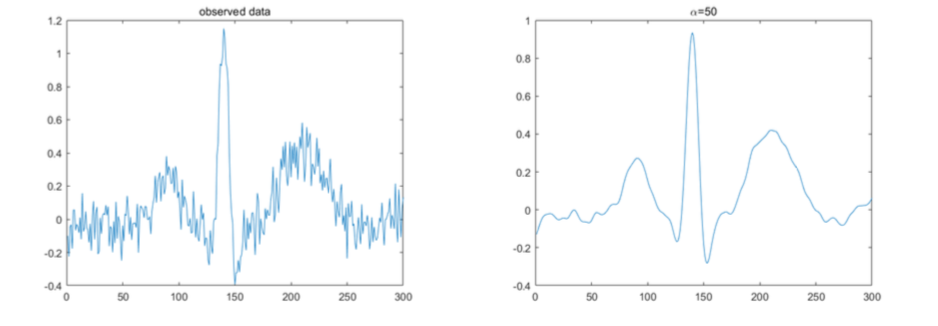
\includegraphics[scale=1]{figuresl/figure3.png}
		\end{center}
	\end{figure}
	\item 图像去模糊\\
	一般模型:
	$$
	f=K(x)+n
	$$
	其中 x 表示真实图像, f 表示观察到的图像,$K(\cdot)$是一个卷积算子, 代表模糊机制, n 代表噪声.
	\item 图像压缩
\end{itemize}


%%%%%%%%%%%%%%%%%%%%%%%%%%%%%%%%%%%%%%%%%%%%%%%%%%%%%%%%%
%%%                      第五章                        %%%
%%%%%%%%%%%%%%%%%%%%%%%%%%%%%%%%%%%%%%%%%%%%%%%%%%%%%%%%%
\subsection{非对称矩阵的特征值问题}
\noindent \textbf{非对称矩阵特征值/特征向量的计算}\\
基本约定1:$A \in \mathbb{R}^{n \times n}$、非对称、稠密\\
基本约定2:~$\left|\lambda_{1}\right| \geq\left|\lambda_{2}\right| \geq \cdots \geq\left|\lambda_{n}\right| \geq 0$\\

本讲主要讨论如何计算 A 的\textcolor{blue}{全部特征值和/或特征向量}\\
主要介绍以下方法:\\
\begin{itemize}
	\item 幂迭代方法
	\item  反迭代方法(位移策略,Rayleigh 商迭代) \item 正交迭代方法
	\item QR方法
\end{itemize}
关于稠密矩阵特征值计算的参考资料有:\\
\begin{itemize}
	\item J.H.Wilkinson,TheAlgebraicEigenvalueProblem,1965
	\item B.N.Parlett,TheSymmetricEigenvalueProblem,2ndEds.,1998
	\item G.W.Stewart,MatrixAlgorithms,VolII:Eigensystems,2001
	\item G.H.GolubandC.F.VanLoan,MatrixComputations,2013
	\item P.Arbenz,Thecourse252-0504-00G,
\end{itemize}
\textcolor{blue}{Numerical Methods for Solving Large Scale Eigenvalue Problems, 2018.
	(该课程的主页)}
\subsection{幂迭代}
\textcolor{blue}{幂迭代} 是计算特征值和特征向量的一种简单易用的算法.\\
虽然简单, 但它却建立了计算特征值和特征向量的算法的一个基本框架.\\
\textcolor{blue}{算法 1.1} 幂迭代算法 (Power Iteration)
\begin{enumerate}[1:]
	\item Choose an initial guess $x(0)$ with $||x(0)||_{2} = 1$
	\item set $k=0$
	\item while not convergence do
	\item \qquad$y^{(k+1)} = Ax^{(k)}$
	\item \qquad$x^{(k+1)}=y^{(k+1)} /\left\|y^{(k+1)}\right\|_{2}$
	\item \qquad$\mu_{k+1}=\left(x^{(k+1)}, A x^{(k+1)}\right)$
	\item \qquad$k=k+1$
	\item end while
\end{enumerate}
幂迭代的收敛性\\
假设1:$A \in \mathbb{R}^{n \times n}$可对角化,即$A=V \Lambda V^{-1}$,其中
$$
\Lambda=\operatorname{diag}\left(\lambda_{1}, \ldots, \lambda_{n}\right), \quad V=\left[v_{1}, \ldots, v_{n}\right] \in \mathbb{C}^{n \times n}, \quad\left\|v_{i}\right\|_{2}=1
$$
假设2:$\left|\lambda_{1}\right|>\left|\lambda_{2}\right| \geq\left|\lambda_{3}\right| \geq \cdots \geq\left|\lambda_{n}\right|$
由于 V 的列向量组构成$\mathbb{C}^{n}$的一组基, 因此$x^{(0)}$可表示为
$$
x^{(0)}=\alpha_{1} v_{1}+\alpha_{2} v_{2}+\cdots+\alpha_{n} v_{n}=V\left[\alpha_{1}, \alpha_{2}, \ldots, \alpha_{n}\right]^{\top}
$$
我们假定$\alpha_{1} \neq 0$,即$x^{(0)}$不属于$\operatorname{span}\left\{v_{2}, v_{3}, \ldots, v_{n}\right\}$
(由于$x^{(0)}$) 是随机选取的, 从概率意义上讲, 这个假设通常是成立的).\\
于是我们可得
$$
A^{k} x^{(0)}=\left(V \Lambda V^{-1}\right)^{k} V\left[\begin{array}{c}{\alpha_{1}} \\ {\alpha_{2}} \\ {\vdots} \\ {\alpha_{n}}\end{array}\right]=V \Lambda^{k}\left[\begin{array}{c}{\alpha_{1}} \\ {\alpha_{2}} \\ {\vdots} \\ {\alpha_{n}}\end{array}\right]=V\left[\begin{array}{c}{\alpha_{1} \lambda_{1}^{k}} \\ {\alpha_{2} \lambda_{2}^{k}} \\ {\vdots} \\ {\alpha_{n} \lambda_{n}^{k}}\end{array}\right]
$$
$$
=\alpha_{1} \lambda_{1}^{k} V\left[\begin{array}{c}{1} \\ {\frac{\alpha_{2}}{\alpha_{1}}\left(\frac{\lambda_{2}}{\lambda_{1}}\right)^{k}} \\ {\vdots} \\ {\frac{\alpha_{n}}{\alpha_{1}}\left(\frac{\lambda_{n}}{\lambda_{1}}\right)^{k}}\end{array}\right]
$$
又$\left|\lambda_{i} / \lambda_{1}\right|<1, i=2,3, \ldots, n$,所以
$$
\lim _{k \rightarrow \infty}\left(\frac{\lambda_{i}}{\lambda_{1}}\right)^{k}=0, \quad i=2,3, \ldots, n
$$
故当 k 趋向于无穷大时, 向量
$$
\left[1, \frac{\alpha_{2}}{\alpha_{1}}\left(\frac{\lambda_{2}}{\lambda_{1}}\right)^{k}, \ldots, \frac{\alpha_{n}}{\alpha_{1}}\left(\frac{\lambda_{n}}{\lambda_{1}}\right)^{k}\right]^{\top}, \quad k=0,1,2, \ldots
$$
收敛到$e_{1}=[1,0, \ldots, 0]^{\top}$\\
所以向量$x^{(k)}=A^{k} x^{(0)} /\left\|A^{k} x^{(0)}\right\|_{2}$收敛到$\pm v_{1}$,即$\lambda_{1}$的特征向量.而$\mu_{k}=\left(x^{(k)}\right)^{*} A x^{(k)}$则收敛到$v_{1}^{*} A v_{1}=\lambda_{1}$
$\dagger$幂迭代的收敛快慢取决于$\left|\lambda_{2} / \lambda_{1}\right|$的大小,$\left|\lambda_{2} / \lambda_{1}\right|$越小,收敛越快.\\
\begin{itemize}
	\item 幂迭代只能用于计算(模)最大的特征值和其相应的特征向量
	\item 当$\left|\lambda_{2} / \lambda_{1}\right|$接近于 1 时, 收敛速度会非常慢
	\item 如果模最大的特征值是一对共轭复数,则幂迭代可能会失效.
\end{itemize}
加速技巧:位移策略\\
出发点: 加快幂迭代算法的收敛速度$\Longleftrightarrow$尽可能地减小$\left|\lambda_{2} / \lambda_{1}\right|$\\
\textcolor{blue}{位移策略:}计算$A-\sigma I$的特征值\\
我们称$\sigma$为\textcolor{blue}{位移},满足
\begin{enumerate}[(1)]
	\item $\lambda_{1}-\sigma$是$A-\sigma I$的模最大特征值
	\item $
	\max _{2 \leq i \leq n}\left|\frac{\lambda_{i}-\sigma}{\lambda_{1}-\sigma}\right|
	$尽可能地小
\end{enumerate}
其中第一个条件保证最后所求得的特征值是我们所要的, 第二个条件用 于加快幂迭代的收敛速度.\\
缺点:(1)$\sigma$很难选取;(2)加速效果有限\\
改进: \textcolor{blue}{与反迭代相结合, 能起到很好的加速效果}
\subsection{反迭代}
\noindent 用幂迭代求$A^{-1}$的模最小特征值,这就是\textcolor{blue}{反迭代}\\
\textcolor{blue}{算法 2.1} 反迭代算法 (Inverse Iteration)\\
\begin{enumerate}[1:]
	\item Choose an initial guess $x(0)$ with $||x(0)||_{2} = 1$
	\item set $k=0$
	\item while not convergence do
	\item \qquad$y^{(k+1)} = (A-\sigma I)^{-1}x^{(k)}$
	\item \qquad$x^{(k+1)}=y^{(k+1)} /\left\|y^{(k+1)}\right\|_{2}$
	\item \qquad$\mu_{k+1}=\left(x^{(k+1)}, A x^{(k+1)}\right)$
	\item \qquad$\sigma=\mu_{k+1},k=k+1$
	\item end while
\end{enumerate}
显然:$\mu_{k}$收敛到$\sigma$最近的特征值,$x^({k})$收敛到对应的特征向量\\
$\dagger$\textcolor{blue}{理论上, 反迭代 + 位移策略, 可以计算矩阵的任意一个特征值}\\
优点:
\begin{itemize}
	\item 若$\sigma$ 与某个特征值 $\lambda_{k}$ 非常接近, 则反迭代算法的收敛速度非常快
	\item 只要选取合适的位移$\sigma$,就可以计算A的任意一个特征值.
\end{itemize}
缺点:
\begin{itemize}
	\item 每步迭代需要解一个线性方程组 $(A-\sigma I) y^{(k+1)}=x^{(k)}$这需要对$A-\sigma I$做LU或PLU分解
	\item 与幂迭代一样,反迭代算法一次只能求一个特征值
	\item 怎样选取位移$\sigma ? \rightarrow$ \textcolor{blue}{Rayleigh 商}动态选取, 自动调整
\end{itemize}
\subsubsection{Rayleigh 商迭代}
\noindent \textcolor{blue}{出发点}:使得 $\sigma$ 与所求的特征值越靠近越好.\\

\textcolor{blue}{期望能直接给出一个理想位移是不太现实的. 比较现实的方法就是动态 调整, 使得位移逐渐靠近某个特征值.}\\
Rayleigh 商迭代: \textcolor{blue}{以 Rayleigh 商 $\mu_{k}$为第 k 步的位移}\\
理由:$\mu_{k}$ 会逐渐收敛到某个特征值.\\

\textcolor{blue}{算法 2.2} Rayleigh 商迭代 (Rayleigh Quotient Iteration, RQI)\\
\begin{enumerate}
	\item Choose an initial vector $x(0)$ with $||x(0)||_{2} = 1$
	\item set $k=0$
	\item compute $\sigma=\left(x^{(0)}\right)^{*} A x^{(0)}$
	\item while not convergence do
	\item \qquad$y^{(k+1)} = (A-\sigma I)^{-1}x^{(k)}$
	\item \qquad$x^{(k+1)}=y^{(k+1)} /\left\|y^{(k+1)}\right\|_{2}$
	\item \qquad$\mu_{k+1}=\left(x^{(k+1)}, A x^{(k+1)}\right)$
	\item \qquad$\sigma=\mu_{k+1}$
	\item \qquad$k=k+1$
	\item end while
\end{enumerate}
RQI 算法的收敛性\\

一般来说, 如果 Rayleigh 商迭代收敛到 A 的一个单特征值, 则至少是二 次收敛的, 即具有局部二次收敛性. 如果 A 是对称的, 则能达到局部三 次收敛, 详情见后面的\textcolor{blue}{对称特征值问题.}\\

缺点:\\
由于每次迭代的位移是不同的, 因此每次迭代需要求解一个不同的线性方程组, 这使得运算量大大增加. \\
因此通常应用于 \textcolor{blue}{三对角矩阵} 的特征值计算
\subsection{正交迭代}
\noindent 出发点:同时计算多个特征值/特征向量\\
策略: 同时采用多个初始向量, 希望收敛到 A 的一个不变子空间\\
\textcolor{blue}{算法 3.1} 正交迭代算法 (Orthogonal Iteration)\\
\begin{enumerate}[1:]
	\item Choose an initial vector$n\times p$column orthogonal matrix $Z_{0}$ 
	\item set $k=0$
	\item while not convergence do
	\item \qquad compute $Y^{(k+1)} = AZ_{(k)}$
	\item \qquad$Y_{(k+1)}=Z_{(k+1)}\hat{R}_{k+1}$
	\item \qquad$k=k+1$
	\item end while
\end{enumerate}
\textcolor{blue}{说明}:\\
在算法中使用 QR 分解是为了保持$z_k$的列正交性, 使得其列向量组构 成子空间 span$\{A^kZ_0\}$的一组正交基. 一方面提高算法的数值稳定性, 另一方面避免所有列都收敛到最大特征值所对应的特征向量.\\
收敛性分析\\
假设 A 是可对角化的, 即$A=V \Lambda V^{-1}$,其中$\Lambda=\operatorname{diag}\left(\lambda_{1}, \lambda_{2}, \ldots, \lambda_{n}\right)$,且$\left|\lambda_{1}\right| \geq \cdots \geq\left|\lambda_{p}\right|>\left|\lambda_{p+1}\right| \geq \cdots \geq\left|\lambda_{n}\right|$.则可得
$$
\operatorname{span}\left\{Z_{k}\right\}=\operatorname{span}\left\{Y_{k}\right\}=\operatorname{span}\left\{A Z_{k-1}\right\}, \quad k=1,2, \ldots
$$
由此可知
$$
\operatorname{span}\left\{Z_{k}\right\}=\operatorname{span}\left\{A^{k} Z_{0}\right\}=\operatorname{span}\left\{V \Lambda^{k} V^{-1} Z_{0}\right\}
$$
我们注意到
$$
\Lambda^{k} V^{-1} Z_{0}=\lambda_{p}^{k}\left[\begin{array}{ccccc}
{\left(\lambda_{1} / \lambda_{p}\right)^{k}} & {} & {} &{}&{}\\ 
{} & {\ddots} & {} & {} &{}\\
{} & {} & {1}& {} & {} \\ 
{} & {} & {} & {\ddots} & {} \\
{} & {} & {} & {} & {\left(\lambda_{n} / \lambda_{p}\right)^{k}}
\end{array}\right]V^{-1} Z_{0} \triangleq \lambda_{p}^{k}\left[\begin{array}{c}
{W_{p}^{(k)}} \\ 
{W_{n-p}^{(k)}}
\end{array}\right]
$$
由于当$i>p$时有$\left|\lambda_{i} / \lambda_{p}\right|<1$,所以当k趋于无穷大时,
$W_{n-p}^{(k)}$趋向于0,令$V=\left[V_{p}, V_{n-p}\right]$,则
$$V \Lambda^{k} V^{-1} Z_{0}=\lambda_{p}^{k}\left[V_{p}, V_{n-p}\right]\left[\begin{array}{c}{W_{p}^{(k)}} \\ {W_{n-p}^{(k)}}\end{array}\right]=\lambda_{p}^{k}\left(V_{p} W_{p}^{(k)}+V_{n-p} W_{n-p}^{(k)}\right)$$
所以当$k \rightarrow \infty$时,有
$$
\begin{aligned} \operatorname{span}\left\{Z_{k}\right\}=\operatorname{span}\left\{V \Lambda^{k} V^{-1} Z_{0}\right\} &=\operatorname{span}\left\{V_{p} W_{p}^{(k)}+V_{n-p} W_{n-p}^{(k)}\right\} \\ & \rightarrow \operatorname{span}\left\{V_{p} W_{p}^{(k)}\right\}=\operatorname{span}\left\{V_{p}\right\} \end{aligned}
$$
即$\operatorname{span}\left\{Z_{k}\right\}$趋向于 A 的一个 $p$ 维不变子空间$\operatorname{span}\left\{V_{p}\right\}$\\

\textcolor{blue}{定理}~~给定正整数$p(1 \leq p \leq n)$,考虑算法3.1,假设A是可对角化的,且$\left|\lambda_{1}\right| \geq \cdots \geq\left|\lambda_{p}\right|>\left|\lambda_{p+1}\right| \geq \cdots \geq\left|\lambda_{n}\right|$.则
$\operatorname{span}\left\{Z_{k}\right\}$收敛到A的一 个 $p$ 维不变子空间.\\
\textcolor{blue}{说明:}\\
如果 A 不可对角化, 利用 Jordan 标准型, 可以到同样的结论, 见 \textcolor{blue}{[Watkins 2007, Watkins-Elsner 1991]}.\\
$\dagger$在正交迭代中, 如果我们取 $Z_{0} = I$, 则可得到一类特殊的正交迭代算 法. 此时, 在一定条件下, 正交迭代会收敛到 $A$ 的 Schur 标准型.
\subsection{QR迭代}

\subsubsection{算法介绍}
\noindent \textcolor{blue}{基本思想}:通过不断的正交相似变换, 将 A 转化为 (拟) 上三角形式\\
\textcolor{blue}{算法 4.1} QR 迭代算法 (QR Iteration)\\
\begin{enumerate}[1:]
	\item Set $A_{1}=A$ and $k=1$
	\item while not convergence do
	\item \qquad $[Q_{k},R_{k}]=qr(A_{k})$
	\item \qquad compute $A_{k+1}=R_{k}Q_{k}$
	\item \qquad$k=k+1$
	\item end while
\end{enumerate}
正交相似性
在 QR 迭代算法中, 我们有
$$
A_{k+1}=R_{k} Q_{k}=\left(Q_{k}^{\top} Q_{k}\right) R_{k} Q_{k}=Q_{k}^{\top}\left(Q_{k} R_{k}\right) Q_{k}=Q_{k}^{\top} A_{k} Q_{k}
$$
由这个递推关系可得
$$
A_{k+1}=Q_{k}^{\top} A_{k} Q_{k}=\cdots=Q_{k}^{\top} Q_{k-1}^{\top} \cdots Q_{1}^{\top} A Q_{1} \cdots Q_{k-1} Q_{k}
$$
记$\tilde{Q}_{k}=Q_{1} \cdots Q_{k-1} Q_{k}$=$\left[\begin{array}{ll}{\tilde{q}_{1}^{(k)},} & {\tilde{q}_{2}^{(k)}, \ldots, \tilde{q}_{n}^{(k)}}\end{array}\right]$
则
\begin{equation} 
A_{k+1}=\tilde{Q}_{k}^{\top} A \tilde{Q}_{k}
\end{equation}
即$A_{k+1}$与$A$正交相似
\subsubsection{QR 迭代与幂迭代的关系}
记$\tilde{R}_{k}=R_{k} R_{k-1} \cdots R_{1}$,则有
$$
\begin{aligned} 
\tilde{Q}_{k} \tilde{R}_{k} &=\tilde{Q}_{k-1}\left(Q_{k} R_{k}\right) \tilde{R}_{k-1}=\tilde{Q}_{k-1}\left(A_{k}\right) \tilde{R}_{k-1} \\ 
&=\tilde{Q}_{k-1}\left(\tilde{Q}_{k-1}^{\top} A \tilde{Q}_{k-1}\right) \tilde{R}_{k-1} \\ 
&=A \tilde{Q}_{k-1} \tilde{R}_{k-1} 
\end{aligned}
$$
由此递推下去, 即可得
$$
\tilde{Q}_{k} \tilde{R}_{k}=A^{k-1} \tilde{Q}_{1} \tilde{R}_{1}=A^{k-1} Q_{1} R_{1}=A^{k}
$$
故
$$
\tilde{Q}_{k} \tilde{R}_{k} e_{1}=A^{k} e_{1}
$$
假设$\left|\lambda_{1}\right|>\left|\lambda_{2}\right| \geq \cdots \geq\left|\lambda_{n}\right|$,则当k充分大时,$A^{k} e_{1}$收敛到A的模最大 特征值 $\lambda_{1}$ 所对应的特征向量.\\
$\rightarrow$ 故$\tilde{Q}_{k}$的第一列$\tilde{q}_{1}^{(k)}$也收敛到 $\lambda_{1}$ 所对应的特征向量\\
因此,当k充分大时,$A \tilde{q}_{1}^{(k)} \rightarrow \lambda_{1} \tilde{q}_{1}^{(k)}$\\
由$A_{k+1}=\tilde{Q}_{k}^{\top} A \tilde{Q}_{k}$可知$A_{k+1}$的第一列
$$
A_{k+1}( :, 1)=\tilde{Q}_{k}^{\top} A \tilde{q}_{1}^{(k)} \rightarrow \lambda_{1} \tilde{Q}_{k}^{\top} \tilde{q}_{1}^{(k)}=\lambda_{1} e_{1}
$$
结论\\
$A_{k+1}$的第一列的第一个元素收敛到$\lambda_{1}$, 而其他元素都趋向于0.收敛速度取决于$|\lambda_{2}/\lambda_{1}|$的大小

\subsubsection{QR迭代与反迭代的关系}
观察$\tilde{Q}_{k}$的最后一列.由$A_{k+1}=\tilde{Q}_{k}^{\top} A \tilde{Q}_{k}$可知
$$
A \tilde{Q}_{k}=\tilde{Q}_{k} A_{k+1}=\tilde{Q}_{k} Q_{k+1} R_{k+1}=\tilde{Q}_{k+1} R_{k+1}
$$
所以有
$$
\tilde{Q}_{k+1}=A \tilde{Q}_{k} R_{k+1}^{-1}
$$
由于$\tilde{Q}_{k+1}$和$\tilde{Q}_{k}$都是正交矩阵,上式两边转置后求逆,可得
$$
\tilde{Q}_{k+1}=\left(\tilde{Q}_{k+1}^{\top}\right)^{-1}=\left(\left(R_{k+1}^{-1}\right)^{\top} \tilde{Q}_{k}^{\top} A^{\top}\right)^{-1}=\left(A^{\top}\right)^{-1} \tilde{Q}_{k} R_{k+1}^{\top}
$$
观察等式两边矩阵的最后一列,可得
$$
\tilde{q}_{n}^{(k+1)}=c_{1}\left(A^{\top}\right)^{-1} \tilde{q}_{n}^{(k)}(c_{1}\text{为某个常数})
$$
以此类推,可知
$$
\tilde{q}_{n}^{(k+1)}=c\left(A^{\top}\right)^{-k} \tilde{q}_{n}^{(1)}(c\text{为某个常数})
$$
假定$\left|\lambda_{1}\right| \geq \cdots \geq\left|\lambda_{n-1}\right|>\left|\lambda_{n}\right|>0$则$\lambda_{n}^{-1}$是$\left(A^{\top}\right)^{-1}$的模最大特征值.由幂迭代可知$\tilde{q}_{n}^{(k+1)}$收敛到$\lambda_{n}^{-1}$所对应的特征向量,即
$$
\left(A^{\top}\right)^{-1} \tilde{q}_{n}^{(k+1)} \rightarrow \lambda_{n}^{-1} \tilde{q}_{n}^{(k+1)} \quad(k \rightarrow \infty)
$$
所以
$$
A^{\top} \tilde{q}_{n}^{(k)} \rightarrow \lambda_{n} \tilde{q}_{n}^{(k)} \quad(k \rightarrow \infty)
$$
由$A_{k+1}=\tilde{Q}_{k}^{\top} A \tilde{Q}_{k}$可知$A_{k+1}^{\top}$的最后一列
$$
A_{k+1}^{\top}( :, n)=\tilde{Q}_{k}^{\top} A^{\top} \tilde{q}_{n}^{(k)} \rightarrow \lambda_{n} \tilde{Q}_{k}^{\top} \tilde{q}_{n}^{(k)}=\lambda_{n} e_{n}
$$
$\mathbf{结论}$\\
$A_{k+1}$的最后一行的最后一个元素收敛到$\lambda_{n}$,而其它元素都趋向于0.收敛速度取决于$\left|\lambda_{n} / \lambda_{n-1}\right|$的大小
\subsubsection{QR 迭代与正交迭代的关系}
下面的定理给出了 QR 迭代算法与正交迭代算法 $(Z_{0} = I)$ 之间的关系.\\
\textcolor{blue}{定理} ~假定正交迭代算法 3.1 和 QR 算法 4.1 中所涉及的 QR 分解都是唯 一的. $A_{k}$ 是由 QR 迭代算法 4.1 生成的矩阵, $Z_{k}$ 是由正交迭代算法 3.1 (取$Z_{0} =I$)生成的矩阵,则有
$$
A_{k+1}=Z_{k}^{\top} A Z_{k}
$$
\subsubsection{QR迭代的收敛性}
\textcolor{blue}{定理}~设$A=V \Lambda V^{-1} \in \mathbb{R}^{n \times n}$,其中$\Lambda=\operatorname{diag}\left(\lambda_{1}, \lambda_{2}, \ldots, \lambda_{n}\right)$,且$\left|\lambda_{1}\right|>\left|\lambda_{2}\right|>\cdots>\left|\lambda_{n}\right|$.若$V^{-1}$的所有顺序主子矩阵都非奇异(即$V^{-1}$存在LU分解),则$A_{k}$的对角线以下的元素收敛到0\\
\textcolor{blue}{说明}:\\
需要指出的是, 由于 $D_{k}$ 的元素不一定收敛, 故 $A_{k+1}$ 对角线以上(不含 对角线)的元素不一定收敛, 但这不妨碍 $A_{k+1}$ 的对角线元素收敛到 A 的特征值(即 $A_{k+1}$ 的对角线元素是收敛的)\\
\textcolor{blue}{例} QR 迭代算法演示 (见$Eig_QR.m$). 设
$$
A=X\left[\begin{array}{cccc}
{9}&&& \\ 
&{5}&& \\
&&3& \\ 
&&&{1}
\end{array}\right] X^{-1}
$$
其中 X 是由 MATLAB 随机生成的非奇异矩阵.\\
在迭代过程中, 对于 Ak 的下三角部分中元素, 如果其绝对值小于某个阈值 tol, 则直接将其设为 0, 即
$$
a_{i j}^{(k)}=0 \quad \text { if } \quad i>j \text { and }\left|a_{i j}^{(k)}\right|<t o l
$$
这里我们取$t o l=10^{-6} \max _{1 \leq i, j \leq n}\left\{\left|a_{i j}^{(k)}\right|\right\}$,迭代过程如下:
\begin{figure}
	\begin{center}
		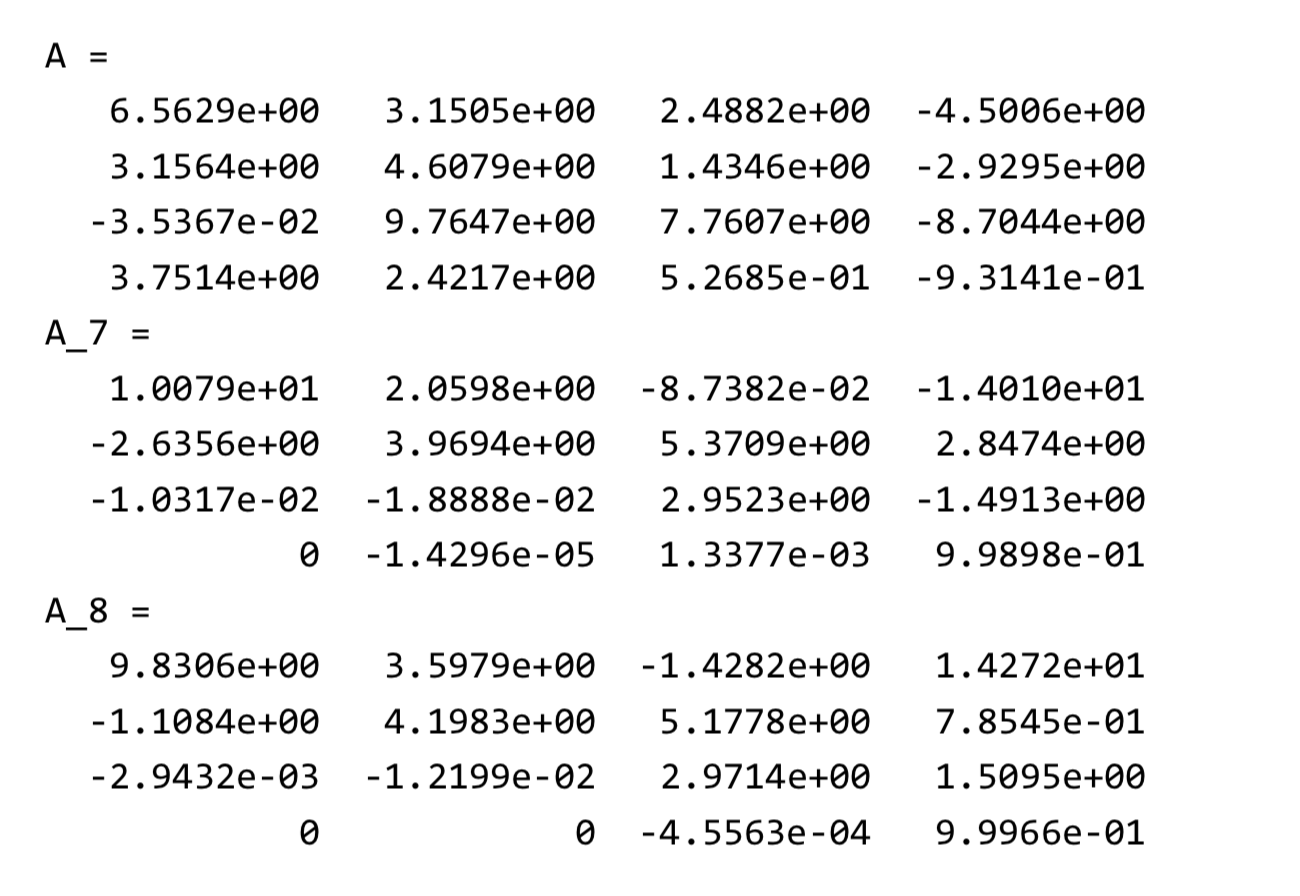
\includegraphics[scale=0.6]{figuresl/figure4.png}
		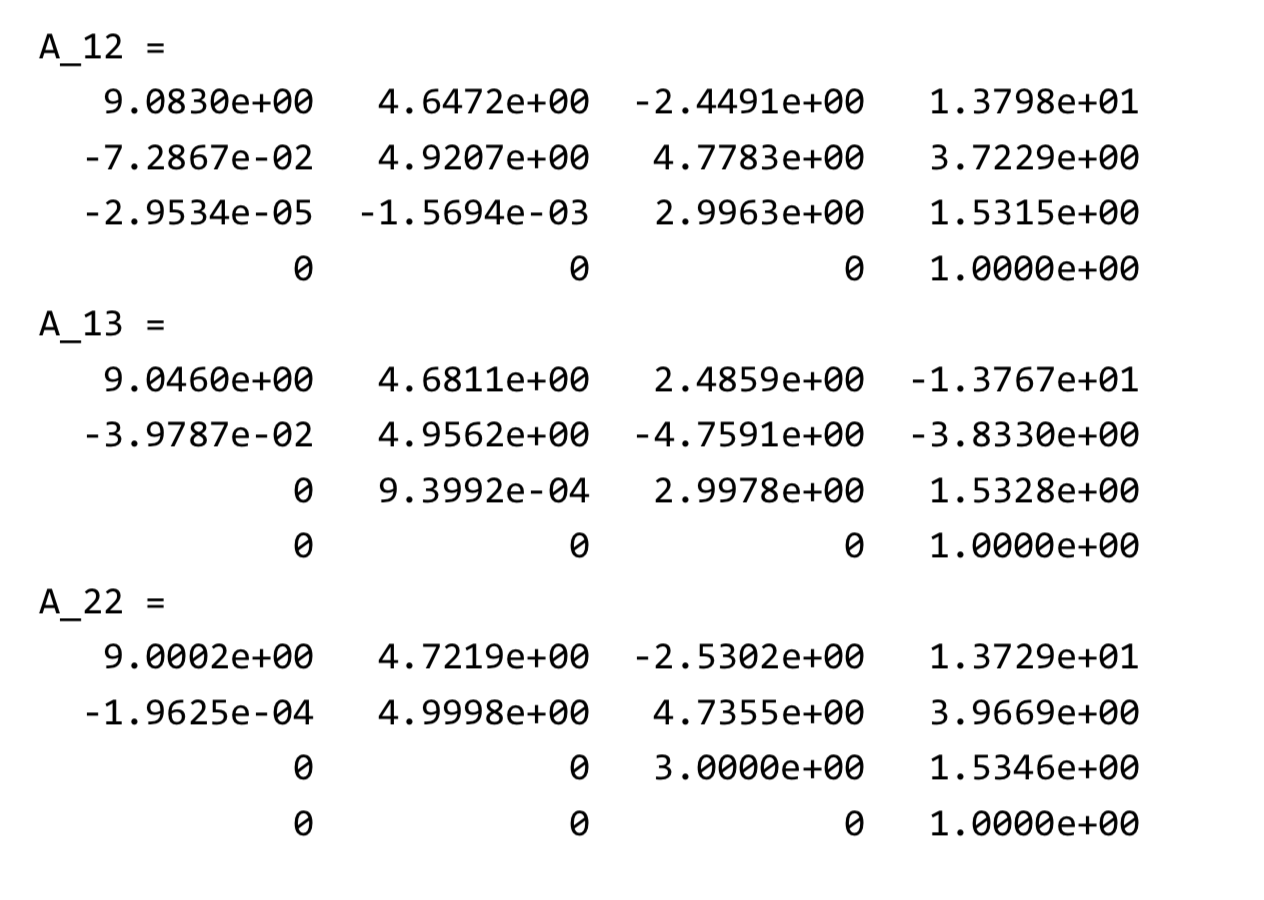
\includegraphics[scale=0.6]{figuresl/figure5.png}
		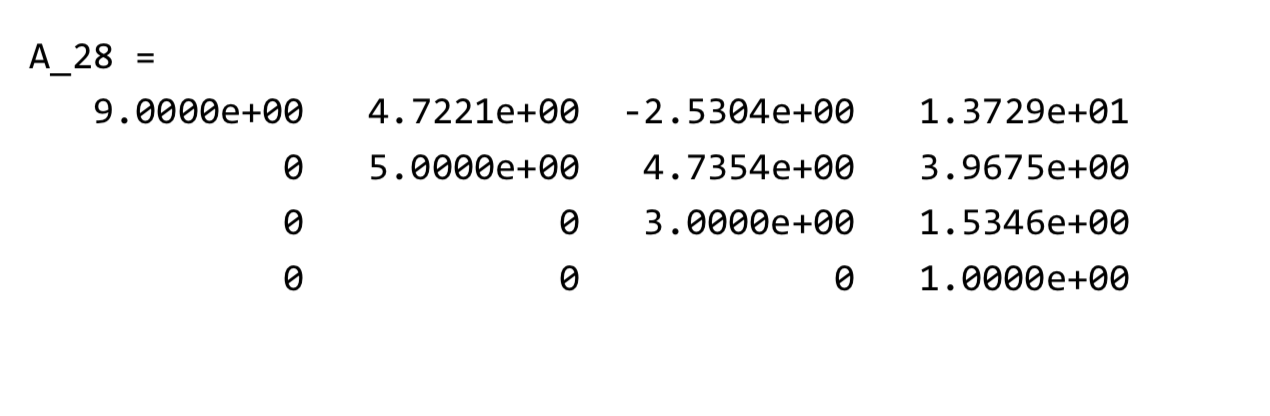
\includegraphics[scale=0.6]{figuresl/figure6.png}
	\end{center}
\end{figure}
\newpage
\subsubsection{带位移的QR迭代}
为了加快 QR 迭代的收敛速度, 可以采用\textcolor{blue}{位移策略} 和\textcolor{blue}{反迭代}的思想\\
\textcolor{blue}{算法 4.2} 带位移的QR 迭代算法 (QR Iteration with shift)\\
\begin{enumerate}[1:]
	\item Set $A_{1}=A$ and $k=1$
	\item while not convergence do
	\item Choose a shift $\sigma_{k}$
	\item \qquad $[Q_{k},R_{k}]=qr(A_{k}-\sigma_{k}I)$
	\item \qquad compute $A_{k+1}=R_{k}Q_{k}+\sigma_{k}I$
	\item \qquad$k=k+1$
	\item end while
\end{enumerate}
正交相似性\\
$$
\begin{aligned} A_{k+1}=R_{k} Q_{k}+\sigma_{k} I &=\left(Q_{k}^{\top} Q_{k}\right) R_{k} Q_{k}+\sigma_{k} I \\ &=Q_{k}^{\top}\left(A_{k}-\sigma_{k} I\right) Q_{k}+\sigma_{k} I \\ &=Q_{k}^{\top} A_{k} Q_{k} \end{aligned}
$$
位移$\sigma_{k}$的选取\\
在前面的分析可知,$A_{k+1}(n, n)$收敛到 A 的模最小特征值.\\
若$\sigma_{k}$就是A的一个特征值,则$A_{k}-\sigma_{k} I$的模最小特征值为0,故QR算 法迭代一步就收敛. 此时
$$
A_{k+1}=R_{k} Q_{k}+\sigma_{k} I=\left[\begin{array}{cc}
{A_{k+1}^{(n-1) \times(n-1)}} & {*} \\
{0} & {\sigma_{k}}
\end{array}\right]
$$
A 的其它特征值可通过对$A_{k+1}^{(n-1) \times(n-1)}$使用带位移 QR 迭代算法得到.\\
通常, 如果 $\sigma_{k}$ 与 A 的某个特征值非常接近, 则收敛速度通常会很快. 由 于 $A_{k} (n, n)$ 收敛到 A 的一个特征值, 所以在实际使用中, 一个比较直观 的位移选择策略是$\sigma_{k} =A_{k}(n,n)$.事实上,这样的位移选取方法通常会 使得 QR 迭代算法有二次收敛速度.\\

\textcolor{blue}{例}~带位移的 QR 迭代算法演示 $(见 Eig_QR_shift.m).$\\
所有数据和设置与例 4.1 相同, 在迭代过程中, 取$\sigma_{k}=A_{k}(n, n)$.如果$A_{k}(n, n)$已经收敛, 则取$\sigma_{k}=A_{k}(n-1, n-1)$
\begin{figure}
	\begin{center}
		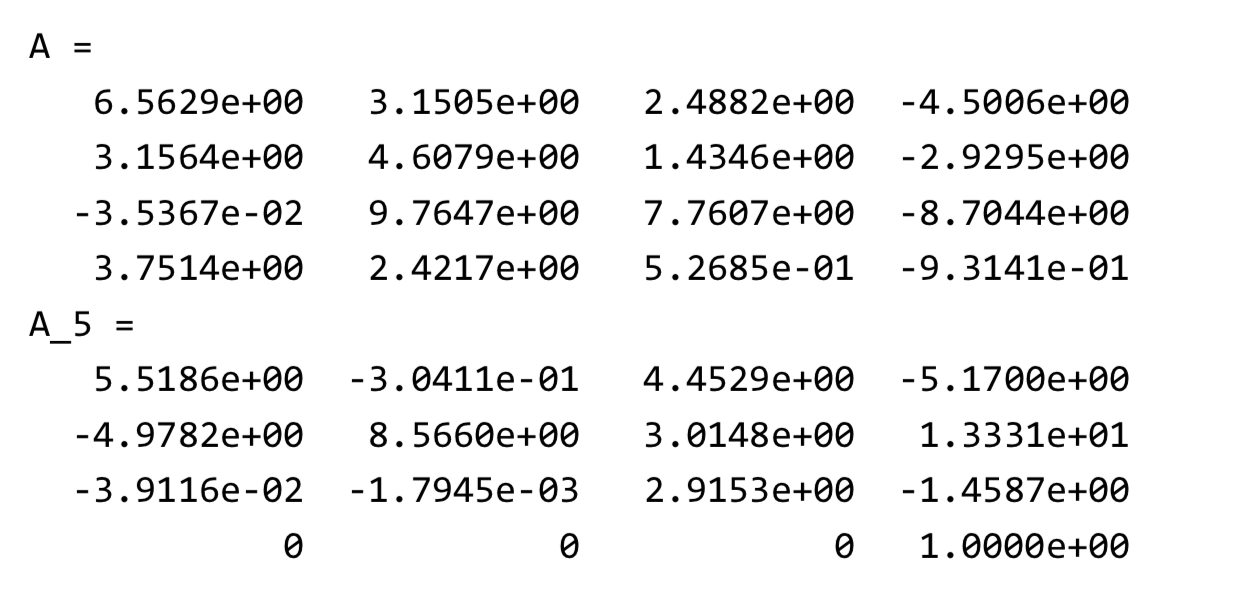
\includegraphics[scale=0.6]{figuresl/figure7.png}
		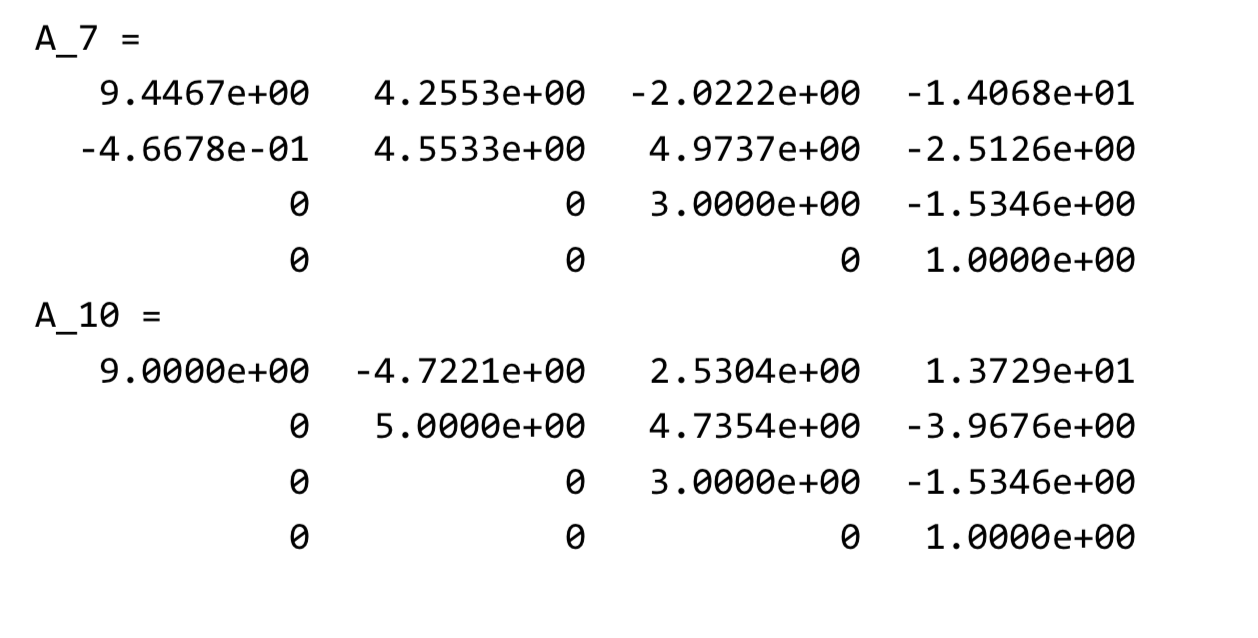
\includegraphics[scale=0.6]{figuresl/figure8.png}
	\end{center}
\end{figure}
\subsection{带位移的隐式QR迭代}
\noindent \textcolor{blue}{直接实施 QR 方法的困难: 运算量}\\
每一步迭代需要做一次 QR 分解和矩阵乘积, 运算量为 $O\left(n^{3}\right)$ 即使每 计算一个特征值只需迭代一步, 则总运算量为$O\left(n^{4}\right)$\\
我们的目标: 从$O\left(n^{4}\right)$减小到$O\left(n^{3}\right)$\\
实现方法:两个步骤\\
\begin{enumerate}[(1)]
	\item 首先通过相似变化将 A 转化成一个 上H
	essenberg 矩阵
	\item 对这个 Hessenberg 矩阵实施 隐式 QR 迭代
\end{enumerate}
\textcolor{blue}{隐式 QR 迭代}:\\
在 QR 迭代算法中, 并 不进行显式的 QR 分解和矩阵乘积 , 而是通过 特殊手段 来实现从$A_{k}$到$A_{k+1}$的迭代,并且将运算量控制在$O\left(n^{2}\right)$量级,从而将总运算量降到$O(n^{3})$
\subsubsection{上 Hessenberg 矩阵}
\noindent \textcolor{blue}{上Hessenberg矩阵:}$H=\left[h_{i j}\right] \in \mathbb{R}^{n \times n}$当$i>j+1$时,有$h_{i j}=0$\\
\textcolor{blue}{定理}设$A \in \mathbb{R}^{n \times n}$,则存在正交矩阵$Q \in \mathbb{R}^{n \times n}$使得$Q A Q^{\top}$是上Hessenberg矩阵\\
下面我们以一个 $5\times 5$ 的矩阵 A 为例, 给出具体的转化过程, 采用的工具 为 Householder 变换.\\
\textcolor{blue}{第一步}:令$Q_{1}=\operatorname{diag}\left(I_{1 \times 1}, H_{1}\right)$,其中$H_{1}$是对应于向量$A(2 : 5,1)$的 Householder 矩阵. 于是可得
$$
Q_{1} A=\left[\begin{array}{ccccc}
* &*& *& *&* \\ 
* &*& *& *&* \\ 
0 &*& *& *&*\\ 
0 &*& *& *&*\\ 
0 &*& *& *&*
\end{array}\right]
$$
由于用$Q_{1}^{T}$右乘$Q_{1} A$,不会改变$Q_{1} A$的第一列元素的值,故
$$
A_{1} \triangleq Q_{1} A Q_{1}^{\top}=\left[\begin{array}{ccccc}
* &*& *& *&* \\ 
* &*& *& *&* \\ 
0 &*& *& *&*\\ 
0 &*& *& *&*\\ 
0 &*& *& *&*
\end{array}\right]
$$
\textcolor{blue}{第二步}:令$Q_{2}=\operatorname{diag}\left(I_{2 \times 2}, H_{2}\right)$,其中$H_{2}$是对应于向量$A_{1}(3 : 5,2)$的 Householder 矩阵, 则用 $Q_{2}$ 左乘 $A_{1} $时, 不会改变 $A_{1}$ 的第一列元素 的值. 用$Q_{2}^{\top}$右乘$Q_{2} A_{1}$时,不会改变$Q_{2} A_{1}$前两列元素的值.因此
$$
Q_{2} A_{1}=\left[\begin{array}{ccccc}
* &*& *& *&* \\ 
* &*& *& *&* \\ 
0 &*& *& *&*\\ 
0 &0& *& *&*\\ 
0 &0& *& *&*
\end{array}\right]和
A_{2}\triangleq Q_{2} A_{1} Q_{2}^{\top}=\left[\begin{array}{ccccc}
* &*& *& *&* \\ 
* &*& *& *&* \\ 
0 &*& *& *&*\\ 
0 &0& *& *&*\\ 
0 &0& *& *&*
\end{array}\right]
$$
\textcolor{blue}{第三步}:
令$Q_{3}=\operatorname{diag}\left(I_{3 \times 3}, H_{3}\right)$,其中$H_{3}$是对应于向量$A_{2}(4 : 5,3)$的Householder 矩阵, 则有
$$
Q_{3} A_{2}=\left[\begin{array}{ccccc}
* &*& *& *&* \\ 
* &*& *& *&* \\ 
0 &*& *& *&*\\ 
0 &0& *& *&*\\ 
0 &0& 0& *&*
\end{array}\right]和A_{3} \triangleq Q_{3} A_{2} Q_{3}^{\top}=\left[\begin{array}{ccccc}
* &*& *& *&* \\ 
* &*& *& *&* \\ 
0 &*& *& *&*\\ 
0 &0& *& *&*\\ 
0 &0& 0& *&*
\end{array}\right]
$$
这时我们就将A转化成一个上Hessenberg矩阵,即
$Q A Q^{\top}=A_{3}$,其中$Q=Q_{3} Q_{2} Q_{1}$是正交矩阵,$A_{3}$是上Hessenberg矩阵.

\textcolor{blue}{第三步:}\quad 令$Q_{3}=\operatorname{diag}\left(I_{3 \times 3}, H_{3}\right)$,其中$H_3$是对应于向量$A_2(4:5,3)$的Householder矩阵,则有$$
Q_{3} A_{2}=\left[\begin{array}{ccccc}{*} & {*} &{*} &{*} & {*} \\ {*} & {*} &{*} &{*} & {*} \\ {0} & {*} &{*} & {*} &{*} \\ {0} & {0} & {*} &{*} & {*} \\ {0} & {0} & {0} & {*} &{*}\end{array}\right]
\text{和} A_{3} \triangleq Q_{3} A_{2} Q_{3}^{\top}=\left[\begin{array}{ccccc}{*} & {*} &{*} &{*} & {*} \\ {*} & {*} &{*} &{*} & {*} \\ {0} & {*} &{*} &{*} & {*} \\  {0} & {0} & {*} &{*} & {*} \\ {0} & {0} & {0} &{*} & {*}\end{array}\right]
$$
这时,我们就将$A$转化成一个上Hessenberg矩阵,即$QAQ^T=A_3$,其中$Q=Q_3Q_2Q_1$是正交矩阵,$A_3$是上Hessenberg矩阵。

上Hessenberg化算法\\
\textcolor{blue}{算法 5.1}\quad 上Hessenberg化算法(Upper Hessenberg Reduction)
\begin{enumerate}[1:]
	\item set $Q=I$
	\item for $k=1$ to $n-2$ do
	\item \quad compute Hessenberg matrix $H_k$ with respect to $A(k+1:n,k)$
	\item \quad $\begin{aligned} A(k+1& : n, k : n )=H_{k} \cdot A(k+1 : n, k : n) \\ &=A(k+1 : n, k : n)-\beta_{k} v_{k}\left(v_{k}^{\top} A(k+1 : n, k : n)\right) \end{aligned}$
	\item \quad $\begin{aligned} A(1 : n, &k+1 : n)=A(1 : n, k+1 : n) \cdot H_{k}^{\top}\\
	&=A(1 : n, k+1 : n)-\beta_{k} A(1 : n, k+1 : n) v_{k} v_{k}^{\top} \end{aligned}$
	\item \quad $\begin{aligned} Q(k+1& : n, k : n )=H_{k} \cdot Q(k+1 : n, k : n) \\ &=Q(k+1 : n, k : n)-\beta_{k} v_{k}\left(v_{k}^{\top} Q(k+1 : n, k : n)\right) \end{aligned}$
	\item end for
\end{enumerate}

\textcolor{blue}{说明:}
\begin{itemize}
	\item 在实际计算时,我们不需要显式地形成Householder矩阵$H_k$。
	\item 上述算法的运算量大约为$\frac{14}{3} n^{3}+\mathcal{O}\left(n^{2}\right)$。如果不需要计算特征向量,则正交矩阵$Q$也不用计算,此时运算量大约为$\frac{10}{3} n^{3}+\mathcal{O}\left(n^{2}\right)$。
	\item 上Hessenberg矩阵的一个很重要的性质就是在QR迭代中保持形状不变。
\end{itemize}

\textcolor{blue}{定理}\quad 设$A \in \mathbb{R}^{n \times n}$是非奇异上Hessenberg矩阵,其QR分解为$A=QR$,则$\tilde{A} \triangleq R Q$也是上Hessenberg矩阵。

若$A$是奇异的,也可以通过选取适当的$Q$,使得上述结论成立。

由此可知,如果$A$是上Hessenberg矩阵,则QR迭代中的每一个$A_k$都是上Hessenberg矩阵矩阵。这样在进行QR分解时,运算量可大大降低。

Hessenberg矩阵另一重要性质:在QR迭代中保持下次对角线元素非零。

\textcolor{blue}{定理}\quad 设$A \in \mathbb{R}^{n \times n}$是上Hessenberg矩阵且下次对角线元素均非零,即$a_{i+1, i} \neq 0, i=1,2, \ldots, n-1$。设其QR分解为$A=QR$,则$\tilde{A} \triangleq R Q$的下次对角线元素也都非零。

若$A$村咋子某个下次对角线元素为零,则$A$一定可约。因此,我们只需考虑下次对角线均非零的情形。

\textcolor{blue}{推论}\quad $\tilde{A} \triangleq R Q$则在带位移的QR迭代中,所有的$A_k$的下次对角线元素均非零。
\subsubsection{隐式QR迭代}
在QR迭代中,我们要先做QR分解$A_k=Q_kR_k$,然后计算$A_{k+1}k=Q_kR_k$.但事实上,我们可以直接计算出$A_{k+1}$。这就是\textcolor{blue}{隐式QR迭代}。

不失一般性,我们假定$A$是不可约的上Hessenberg矩阵。

隐式QR迭代的理论基础就是下面的\textcolor{blue}{隐式Q定理}。

\textcolor{blue}{定理(ImplicitQTheorem)}\quad 设$H=Q^{\top} A Q \in \mathbb{R}^{n \times n}$是一个不可约上Hessenberg矩阵,其中$Q \in \mathbb{R}^{n \times n}$是正交矩阵,则$Q$的第$2$至第$n$列均由$Q$的第一列所唯一确定(可相差一个符号)。

由于$Q_k$的其他列都由$Q_k$的第一列唯一确定(至多相差一个符号),所以我们只要找到一个正交矩阵$\tilde{Q}_{k}$使得其第一列与$\tilde{Q}_{k}$的第一列相等,且$\tilde{Q}_{k}^{\top} A_{k} \tilde{Q}_{k}$为上Hessenberg矩阵,则由隐式$Q$定理可知$\tilde{Q}_{k}=W Q_{k}$,其中$W=\operatorname{diag}(1, \pm 1, \ldots, \pm 1)$,于是$$
\tilde{Q}_{k}^{\top} A_{k} \tilde{Q}_{k}=W^{\top} Q_{k}^{\top} A_{k} Q_{k} W=W^{\top} A_{k+1} W
$$。
又$W^{\top} A_{k+1} W$与$A_{k+1}$相似,且对角线元素相等,而其他元素也至多相差一个符号,所以不会影响$A_{k+1}$的收敛性,即下三角元素收敛到$0$,对角线元素收敛到$A$的特征值。

在QR迭代算法中,如果我们直接令$A_{k+1}=\tilde{Q}_{k}^{\top} A_{k} \tilde{Q}_{k}$,则其收敛性与原QR迭代算法没有任何区别!这就是隐式QR迭代的基本思想。

由于$A$是上Hessenberg矩阵,因此在实际计算中,我们只需Givens变换。

下面我们举一个例子,具体说明如何利用隐式Q定理,由$A_1$得到$A_2$。

设$A \in \mathbb{R}^{5 \times 5}$是一个不可约上Hessenberg矩阵,即$$
A_{1}=A=\left[\begin{array}{ccccc}{*} & {*} & {*}& {*}& {*} \\ {*} & {*} & {*}& {*}& {*} \\ {0} & {*} & {*}& {*}& {*} \\ {0} & {0} & {*} & {*}& {*} \\ {0} & {0} & {0} & {*}& {*}\end{array}\right]
$$
\textcolor{blue}{第一步:}\quad 构造一个Givens变换
$$
G_{1}^{\top} \triangleq G\left(1,2, \theta_{1}\right)=\left[\begin{array}{ccc}{c_{1}} & {s_{1}}& \\ {-s_{1}} & {c_{1}} &\\ {} && {I_{3}}\end{array}\right]
\qquad (c_1,s_1\text{待定})
$$
于是有$$
G_{1}^{\top} A=\left[\begin{array}{ccccc}{*}  & {*} & {*}& {*}& {*}\\ {*} & {*} & {*} & {*}& {*}\\ {0} & {*} & {*}& {*}& {*} \\ {0} & {0} & {*} & {*}& {*}\\ {0} & {0} & {0} & { *}& {*}\end{array}\right] \text{和}A^{(1)} \triangleq G_{1}^{\top} A G_{1}=\left[\begin{array}{ccccc}{*}  & {*} & {*}& {*} & {*} \\ {*}  & {*} & {*}& {*} & {*} \\ {+} & {*} & {*}  & {*} & {*}\\ {0} & {0} & {*} & {*}  & {*}\\ {0} & {0} & {0} & {*} & {*}\end{array}\right]
$$
与$A_1$相比较,$A^{(1)}$在$(3,1)$位置上多出一个非零元,我们把它记为“+”,并称之为\textcolor{blue}{bulge}。在下面的计算过程中,我们的目标就是将其“赶”出矩阵,从而得到一个新的上Hessenberg矩阵,即$A_2$。

\textcolor{blue}{第二步:}\quad 为了消去这个bulge,我们可以构造Givens变换$$
G_{2}^{\top} \triangleq G\left(2,3, \theta_{2}\right)=\left[\begin{array}{cccc}{1} & {} & {} &\\ {} & {c_{2}} & {s_{2}}& \\ {} & {-s_{2}} & {c_{2}} &\\ {} & {} && {I_{2}}\end{array}\right]
\text{使得}G_{2}^{\top} A^{(1)}=\left[\begin{array}{ccccc}{*} & {*} & {*} & {*}& {*}\\ {*} & {*} & {*} & {*} & {*}\\ {0} & {*} & {*} & {*}& {*} \\ {0} & {0} & {*} & {*}& {*} \\ {0} & {0} & {0} & {*}& {*}\end{array}\right]$$

为了保持与原矩阵的相似性,需要再右乘$G_2$,所以$$
A^{(2)} \triangleq G_{2}^{\top} A^{(1)} G_{2}=\left[\begin{array}{ccccc}{*} & {*} & {*} & {*}& {*}\\ {*} & {*} & {*} & {*}& {*}\\ {0} & {*} & {*}& {*}& {*} \\ {0} & {+} & {*} & {*}& {*}\\ {0} & {0} & {0} & {*}& {*}\end{array}\right]
$$
此时,bugle从$(3,1)$位置被“赶”到$(4,2)$位置。

\textcolor{blue}{第三步:}\quad 与第二步类似,构造Givens变换$$
G_{3}^{\top} \triangleq G\left(3,4, \theta_{3}\right)=\left[\begin{array}{cccc}{I_{2}} & {} & {}& {} \\ {} & {c_{3}} & {s_{3}} & {}\\ {} & {-s_{3}}& { c_{3}} & {}\\ {} & {}& {} & {1}\end{array}\right]
\text{使得}G_{3}^{\top} A^{(2)}=\left[\begin{array}{ccccc}{*} & {*} & {*} & {*}& {*}\\ {*} & {*} & {*} & {*} & {*}\\ {0} & {*} & {*} & {*}& {*} \\ {0} & {0} & {*} & {*}& {*} \\ {0} & {0} & {0} & {*}& {*}\end{array}\right]
$$这时$$
A^{(3)} \triangleq G_{3}^{\top} A^{(2)} G_{3}=\left[\begin{array}{ccccc}{*} & {*} & {*} & {*}& {*}\\ {*} & {*} & {*} & {*}& {*}\\ {0} & {*} & {*}& {*}& {*} \\ {0} & {0} & {*} & {*}& {*}\\ {0} & {0} & {+} & {*}& {*}\end{array}\right]
$$
于是,bugle又从$(4,2)$位置被“赶”到$(5,3)$位置。

\textcolor{blue}{第四步:}\quad 再次构造Givens变换$$
G_{4}^{\top} \triangleq G\left(4,5, \theta_{4}\right)=\left[\begin{array}{ccccc}{1} & {} & {}& {} &\\ {} & {1} & {} & {}&\\ {} & {}& {1} & {}&\\ {} & {}& {} & {c_4}&s_4\\{} & {}& {} & {-s_4}&c_4\end{array}\right]
\text{使得}G_{4}^{\top} A^{(3)}=\left[\begin{array}{ccccc}{*} & {*} & {*} & {*}& {*}\\ {*} & {*} & {*} & {*} & {*}\\ {0} & {*} & {*} & {*}& {*} \\ {0} & {0} & {*} & {*}& {*} \\ {0} & {0} & {0} & {*}& {*}\end{array}\right]
$$这时$$
A^{(4)} \triangleq G_{4}^{\top} A^{(3)} G_{4}=\left[\begin{array}{ccccc}{*} & {*} & {*} & {*}& {*}\\ {*} & {*} & {*} & {*}& {*}\\ {0} & {*} & {*}& {*}& {*} \\ {0} & {0} & {*} & {*}& {*}\\ {0} & {0} & {0} & {*}& {*}\end{array}\right]
$$
现在,bulge被“赶”出矩阵,$A{(4)}$就是我们所要的矩阵!\\
\textbf{算法分析,以及$c_1,s_1$的取值}

常规QR迭代:$A_{1}=Q_{1} R_{1}, A_{2}=R_{1} Q_{1} \Longrightarrow A_{2}=Q_{1}^{\top} A_{1} Q_{1}$

根据前面的计算过程,有$$
A^{(4)}=G_{4}^{\top} G_{3}^{\top} G_{2}^{\top} G_{1}^{\top} A_{1} G_{1} G_{2} G_{3} G_{4}=\tilde{Q}_{1}^{\top} A_{1} \tilde{Q}_{1}
$$,其中$\tilde{Q}_{1}=G_{1} G_{2} G_{3} G_{4} \Longrightarrow A^{(4)}=\tilde{Q}_{1}^{\top} A_{1} \tilde{Q}_{1}$

通过直接计算可知,$\tilde{Q}_{1}$的第一列为$$
\left[c_{1}, s_{1}, 0,0,0\right]^{\top}
$$

如果将其取为$A_1$的第一列$\left[a_{11}, a_{21}, 0, \ldots, 0\right]^{\top}$单位化后的向量,\textcolor{blue}{则$\tilde{Q}_{1}$的第一列与$Q_{1}$的第一列相同!$\Longrightarrow A^{(4)}=W^{\top} A_{2} W$}

针对带位移的QR方法,我们取$A_{1}-\sigma_{1} I$的第一列$$
\left[a_{11}-\sigma_{1}, a_{21}, 0, \ldots, 0\right]^{\top}
$$单位化后的向量作为$G_1$的第一列即可。\\
\textcolor{blue}{运算量:}

如果$A \in \mathbb{R}^{n \times n}$是上Hessenberg矩阵,则使用上面的算法,带位移QR迭代中每一步的运算量为$6 n^{2}+O(n)$。

\subsubsection{位移的选取}
通常,位移越离某个特征值越近,则收敛速度就越快。

由习题4.10可知,如果位移$\sigma$与某个特征值非常接近,则$A_{k}(n, n)-\sigma$就非常接近于0。

这说明\textcolor{blue}{$A_k(n,n)$通常会首先收敛到$A$的一个特征值。}所以\textcolor{blue}{$\sigma=A_{k}(n, n)$是一个不错的选择。}但是,如果这个特征值是复数,这种唯一选取方法就可能失效。

\textbf{双位移策略}

设$\sigma \in \mathbb{C}$是$A$的某个复特征值$\lambda$的一个很好的近似,则其共轭$\overline{\sigma}$也应该是$\overline{\lambda}$的一个很好的近似。因此我们可以考虑\textcolor{blue}{双位移}策略,即先以$\lambda$为位移迭代一次,然后再以$\overline{\sigma}$为位移迭代一次,如此不断交替进行迭代。

这样就有$$
\begin{aligned} A_{1}-\sigma I &=Q_{1} R_{1} \\ A_{2} &=R_{1} Q_{1}+\sigma I \\ A_{2}-\overline{\sigma} I &=Q_{2} R_{2} \\ A_{3} &=R_{2} Q_{2}+\overline{\sigma} I \end{aligned}
$$容易验证$$
A_{3}=Q_{2}^{\top} A_{2} Q_{2}=Q_{2}^{*} Q_{1}^{*} A_{1} Q_{1} Q_{2}=Q^{*} A_{1} Q
$$其中$Q=Q_1Q_2$

我们注意到$\sigma$可能是复的,所以$Q_1$和$Q_2$都可能是复矩阵。但我们却可以选取适当的$Q_1$和$Q_2$,使得$Q=Q_1Q_2$是实矩阵。

\textbf{双位移策略的实现}

由前面的结论可知,存在$Q_1$和$Q_2$,使得$Q=Q_1Q_2$是实矩阵,从而$$
A_{3}=Q^{\top} A_{1} Q
$$也是实矩阵。因此我们希望\textcolor{blue}{不计算$A_2$,而是直接从$A_1$得到$A_3$}\\
\textcolor{blue}{实现方式:}

根据隐式Q定理:只要找到一个实正交矩阵$Q$,使得其第一列与$$
A_{1}^{2}-2 \operatorname{Re}(\sigma) A_{1}+|\sigma|^{2} I
$$的第一列平行,并且$A_{3}=Q^{\top} A_{1} Q$是上Hessenberg矩阵即可。

易知,$A_{1}^{2}-2 \operatorname{Re}(\sigma) A_{1}+|\sigma|^{2} I$的第一列为\begin{equation}
\left[\begin{array}{c}{a_{11}^{2}+a_{12} a_{21}-2 \operatorname{Re}(\sigma) a_{11}+|\sigma|^{2}} \\ {a_{21}\left(a_{11}+a_{22}-2 \operatorname{Re}(\sigma)\right)} \\ {a_{21} a_{32}} \\ {0} \\ {\vdots}\end{array}\right]
\end{equation}
所以$Q$的第一列是上述向量的单位化。

其他过程可以通过隐式QR迭代来实现。但此时的“bulge"是一个$2\times 2$的小矩阵。因此,在双位移隐式R迭代过程中,\textcolor{blue}{需要使用Householder变换。}

需要指出的是,\textcolor{blue}{双位移QR迭代算法中的运算都是实数运算。}

下面通过一个例子来说明如何在实数运算下实现双位移隐式QR迭代。

设$A \in \mathbb{R}^{6 \times 6}$是一个不可约上Hessenberg矩阵,即$$
A_{1}=A=\left[\begin{array}{cccccc}{*} & {*} & {*}  & {*} & {*} & {*}\\ {*} & {*} & {*} & {*} & {*} & {*} \\ {0} & {*} & {*} & {*}  & {*} & {*}\\ {0} & {0} & {*} & {*} & {*} & {*} \\ {0}& {0}  & {0} & {*} & {*}  & {*} \\ {0} & {0} & {0} & {0} & {*} & {*}\end{array}\right]
$$

\textcolor{blue}{第一步:}\quad 构造一个正交矩阵$H_{1}=\left[\begin{array}{cc}{\tilde{H}_{1}^{\top}} & {0} \\ {0} & {I_{3}}\end{array}\right]$,其中$\tilde{H}_{1} \in \mathbb{R}^{3 \times 3}$,使得第一列与$A_{1}^{2}-2 \operatorname{Re}(\sigma) A_{1}+|\sigma|^{2} I$的第一列平行。于是有$$
H_{1}^{\top} A=\left[\begin{array}{cccccc}{*} & {*} & {*} & {*} & {*}& {*}\\ {*} & {*} & {*} & {*}& {*}& {*} \\ {+} & {*} & {*} & {*}& {*}& {*} \\ {0} & {0} & {*} & {*}& {*}& {*} \\ {0} & {0} & {0} & {*} & {*}& {*}\\ {0} & {0} & {0} & {0} & {*}& {*}\end{array}\right]
\text{和}A^{(1)} \triangleq H_{1}^{\top} A H_{1}=\left[\begin{array}{cccccc}{*} & {*} & {*} & {*}& {*}& {*} \\ {*} & {*} & {*} & {*}& {*}& {*} \\ {+} & {*} & {*} & {*}& {*}& {*} \\ {+} & {+} & {*}& {*} & {*} & {*}  \\ {0} & {0} & {0} & {*} & {*}& {*} \\ {0} & {0} & {0} & {0 }& {*}& {*}\end{array}\right]
$$
与$A_1$相比较,$A^{(1)}$在$(3,1),(4,1)$和$(4,2)$位置上出现bulge。在下面的计算过程中,我们的目标就是把它们”赶“出矩阵,从而得到一个新的上Hessenberg矩阵。

\textcolor{blue}{第二步:}\quad 令$H_{2}=\left[\begin{array}{ccc}{1} & {0} & {0} \\ {0} & {\tilde{H}_{2}^{\top}} & {0} \\ {0} & {0} & {I_{2}}\end{array}\right]$,其中$\tilde{H}_{2} \in \mathbb{R}^{3 \times 3}$是对应于$A(2 : 4,1)$的Householder变换,使得$$
H_{2}^{\top} A^{(1)}=\left[\begin{array}{cccccc}{*} & {*} & {*}& {*}& {*}& {*} \\ {*} & {*} & {*} & {*}& {*}& {*}\\ {0} & {*} & {*} & {*} & {*}& {*}\\ {0} & {+} & {*} & {*}& {*}& {*}\\ {0} & {0} & {0} & {*}& {*}& {*}\\ {0} & {0} & {0} & {0}& {*}& {*}\end{array}\right]
\text{和}A^{(2)} \triangleq H_{2}^{\top} A^{(1)} H_{2}=\left[\begin{array}{cccccc}{*} & {*} & {*}& {*}& {*}& {*} \\ {*} & {*} & {*} & {*}& {*}& {*}\\ {0} & {*} & {*} & {*} & {*}& {*}\\ {0} & {+} & {*} & {*}& {*}& {*}\\ {0} & {+} & {+} & {*}& {*}& {*}\\ {0} & {0} & {0} & {0}& {*}& {*}\end{array}\right]
$$
这时,我们将bugle向右下角方向”赶“了一个位置。

\textcolor{blue}{第三步}\quad 与第二步类似,令$H_{3}=\left[\begin{array}{ccc}{I_2} & {0} & {0} \\ {0} & {\tilde{H}_{3}^{\top}} & {0} \\ {0} & {0} & {1}\end{array}\right]$,其中$\tilde{H}_{3} \in \mathbb{R}^{3 \times 3}$是对应于$A(3 : 5,2)$的Householder变换,使得$$
H_{3}^{\top} A^{(2)}=\left[\begin{array}{cccccc}{*} & {*} & {*}& {*}& {*}& {*} \\ {*} & {*} & {*} & {*}& {*}& {*}\\ {0} & {*} & {*} & {*} & {*}& {*}\\ {0} & {0} & {*} & {*}& {*}& {*}\\ {0} & {0} & {+} & {*}& {*}& {*}\\ {0} & {0} & {0} & {0}& {*}& {*}\end{array}\right]
\text{和}A^{(3)} \triangleq H_{3}^{\top} A^{(2)} H_{3}=\left[\begin{array}{cccccc}{*} & {*} & {*}& {*}& {*}& {*} \\ {*} & {*} & {*} & {*}& {*}& {*}\\ {0} & {*} & {*} & {*} & {*}& {*}\\ {0} & {0} & {*} & {*}& {*}& {*}\\ {0} & {0} & {+} & {*}& {*}& {*}\\ {0} & {0} & {+} & {+}& {*}& {*}\end{array}\right]
$$
这时,bugle又被向右下角方向”赶“了一个位置。

\textcolor{blue}{第四步}\quad 令$H_{4}=\left[\begin{array}{cc}{I_3} & {0} \\ {0} & {\tilde{H}_{4}^{\top}}  \end{array}\right]$,其中$\tilde{H}_{4} \in \mathbb{R}^{3 \times 3}$是对应于$A(4: 6,3)$的Householder变换,使得$$
H_{4}^{\top} A^{(3)}=\left[\begin{array}{cccccc}{*} & {*} & {*}& {*}& {*}& {*} \\ {*} & {*} & {*} & {*}& {*}& {*}\\ {0} & {*} & {*} & {*} & {*}& {*}\\ {0} & {0} & {*} & {*}& {*}& {*}\\ {0} & {0} & {0} & {*}& {*}& {*}\\ {0} & {0} & {0} & {+}& {*}& {*}\end{array}\right]
\text{和}A^{(4)} \triangleq H_{4}^{\top} A^{(3)} H_{4}=\left[\begin{array}{cccccc}{*} & {*} & {*}& {*}& {*}& {*} \\ {*} & {*} & {*} & {*}& {*}& {*}\\ {0} & {*} & {*} & {*} & {*}& {*}\\ {0} & {0} & {*} & {*}& {*}& {*}\\ {0} & {0} & {0} & {*}& {*}& {*}\\ {0} & {0} & {0} & {+}& {*}& {*}\end{array}\right]
$$

\textcolor{blue}{第五步}\quad 只需构造一个Givens变换$G_{5}=\left[\begin{array}{cc}{I_4} & {0} \\ {0} & {G(4,5,\theta)^{\top}}  \end{array}\right]$,使得$$
G_{}5^{\top} A^{(4)}=\left[\begin{array}{cccccc}{*} & {*} & {*}& {*}& {*}& {*} \\ {*} & {*} & {*} & {*}& {*}& {*}\\ {0} & {*} & {*} & {*} & {*}& {*}\\ {0} & {0} & {*} & {*}& {*}& {*}\\ {0} & {0} & {0} & {*}& {*}& {*}\\ {0} & {0} & {0} & {0}& {*}& {*}\end{array}\right]
\text{和}A^{(5)} \triangleq G_{5}^{\top} A^{(4)} G_{5}=\left[\begin{array}{cccccc}{*} & {*} & {*}& {*}& {*}& {*} \\ {*} & {*} & {*} & {*}& {*}& {*}\\ {0} & {*} & {*} & {*} & {*}& {*}\\ {0} & {0} & {*} & {*}& {*}& {*}\\ {0} & {0} & {0} & {*}& {*}& {*}\\ {0} & {0} & {0} & {0}& {*}& {*}\end{array}\right]
$$

现在,bulge已经被全部消除,且$$A^{(5)}=Q^{\top} A Q$$,其中$Q=H_{1} H_{2} H_{3} H_{4} G_{5}$。通过直接计算可知,$Q$的第一列即为$H_1$的第一列。根据隐式Q定理,可以直接令$A_{3} \triangleq A^{(5)}=Q^{\top} A Q$。

\textbf{位移的具体选取}

在单位移QR迭代算法中,若$A$的特征值都是实的,则取$\sigma_{k}=A_{k}(n, n)$.推广到复共轭特征值上,我们可以取$A_k$的右下角矩阵$$
\left[\begin{array}{cc}{A_{k}(n-1, n-1)} & {A_{k}(n-1, n)} \\ {A_{k}(n, n-1)} & {A_{k}(n, n)}\end{array}\right]
$$的复共轭特征值作为双位移。这样选取的位移就是\textcolor{blue}{Francis位移}。

如果上述矩阵的两个特征值都是实的,则选取其中模较小的特征值做单位移。

采用Francis位移的QR迭代会使得$A_k$的右下角收敛到一个上三角矩阵(两个实特征值)或一个2阶的矩阵(一对复共轭特征值),而且通常会有二次收敛性。在实际计算中,一个特征值一般平均只需迭代两步。\\
\textcolor{blue}{收敛性判断:}

判断收敛性主要是看$A_{k}(n-1, n-2)$(或$A_{k}(n, n-1)$)是否趋向于$0$。

需要指出的是,QR迭代并不是对所有的矩阵都收敛。例如:$$A=\left[\begin{array}{lll}{0} & {0} & {1} \\ {1} & {0} & {0} \\ {0} & {1} & {0}\end{array}\right]$$
对于上面的矩阵,采用Francis位移的QR迭代算法无效。另外,也可以考虑多重位移策略,参见\textcolor{blue}{[Watkins 2007]}。
\subsubsection{收缩Deflation}
收缩(deflation)技术是实用QR迭代中的一个非常重要概念。

隐式QR迭代过程中,当矩阵$A_{k+1}$的某个下次对角线元素$a_{i+1}$,$i$很小时,我们可以将其设为$0$。

由于$A_{k+1}$是上Hessenberg矩阵,这时$A_{k+1}$就可以写成分块上三角形式,其中两个对角块都是上Hessenberg矩阵。

因此我们可以将隐式QR迭代作用在这两个规模相对较小的矩阵上,从而可以大大节约运算量。
\subsection{特征向量的计算}
设$A$的特征值都是实的,$R=Q^TAQ$是其Schur标准型。若$Ax=\lambda x$,则 $Ry=\lambda y$,其中$y=Q^Tx$或$x=Qy$。故只需计算R的特征向量$y$即可。

因为$R$的对角线元素即为$A$的特征值,不妨设$\lambda=R(i,i)$。

假定$\lambda$是单重特征值,则方程$(R-\lambda I)y=0$即为$$
\left[\begin{array}{ccc}{R_{11}-\lambda I R_{12}} & {R_{13}} \\ {0} & {0} & {R_{23}} \\ {0} & {0} & {R_{33}-\lambda I}\end{array}\right]\left[\begin{array}{l}{y_{1}} \\ {y_{2}} \\ {y_{3}}\end{array}\right]=0
$$即\begin{equation}
\left(R_{11}-\lambda I\right) y_{1}+R_{12} y_{2}+R_{13} y_{3}=0
\end{equation}\begin{equation}
R_{23} y_{3}=0
\end{equation}\begin{equation}
\left(R_{33}-\lambda I\right) y_{3}=0
\end{equation}其中$R_{11} \in \mathbb{R}^{(i-1) \times(i-1)}, R_{33} \in \mathbb{R}^{(n-i) \times(n-i)}$。由于$\lambda$是单重特征值,故
$R_{33}-\lambda I$非奇异,因此$y_3=0$。令$y_2=1$,则可得$$
y_{1}=\left(R_{11}-\lambda I\right)^{-1} R_{12}
$$

因此计算特征向量$y$只需求解一个上三角线性方程组。

若$\lambda$是多重特征值,则据算方法类似。但如果$A$有负特征值,则需要利用实Schur标准型,计算较复杂。
\subsection{广义特征值问题}
设$A, B \in \mathbb{R}^{n \times n}$,若存在$\lambda \in \mathbb{C}$和非零向量$x \in \mathbb{C}^{n}$使得$$
A x=\lambda B x
$$则称$\lambda$为矩阵对$(A,B)$的特征值,$x$为对应的特征向量。

计算矩阵对$(A,B)$的特征值和特征向量就是\textcolor{blue}{广义特征值问题}

当$B$非奇异时,广义特征值问题就等价于标准特征值问题$$
B^{-1} A x=\lambda x
\text{或}A B^{-1} y=\lambda y
$$其中$y=Bx$。

容易看出,$\lambda$是$(A,B)$的一个特征值当且仅当\begin{equation}
\operatorname{det}(A-\lambda B)=0
\label{equation4.9}
\end{equation}

若\ref{equation4.9}对所有$\lambda \in \mathbb{C}$都成立,则称矩阵对$(A,B)$是\textcolor{blue}{奇异矩阵对},否则称为\textcolor{blue}{正则矩阵对}。

当$B$非奇异时,特征方程\ref{equation4.9}是一个$n$次多项式,因此恰好有$n$个特好找呢个字。当$B$奇异时,特征方程\ref{equation4.9}的次数低于$n$,因此方程的解的个数小于$n$。但是,注意带$\lambda \neq 0$是$(A,B)$的t特征值当且仅当$\mu=\frac{1}{\lambda}$是$(B, A)$的特征值。因此,当$B$奇异时,$\mu=0$是$(B, A)$的特征值,于是我们自然的把$\lambda=\frac{1}{u}=\infty$当作是$(A,B)$的特征值。所以广义特征值不是分布在$\mathbb{C}$上,而是分布在$\mathbb{C} \cup\{\infty\}$上。

容易验证,若$U,V$非奇异,则矩阵对$\left(U^{*} A V, U^{*} B V\right)$的特征值与$(A,B)$是一样的。因此我们称这种变换为\textcolor{blue}{矩阵对的等价变换}。如果$U,V$是酉矩阵,则称为\textcolor{blue}{酉等价变换}。
\subsubsection{广义Schur分解}
\textcolor{blue}{广义Schur分解}是矩阵对在酉等价变换下的最简形式。

\textcolor{blue}{定理(广义Schur分解)}\quad 设$A, B \in \mathbb{C}^{n \times n}$,则存在酉矩阵$Q, Z \in \mathbb{C}^{n \times n}$,使得\begin{equation}
Q^{*} A Z=R_{A}, \quad Q^{*} B Z=R_{B}
\end{equation}其中$R_{A}, R_{B} \in \mathbb{C}^{n \times n}$都是上三角矩阵。此时矩阵对$(A,B)$的特征值为$R_A$和$R_B$的对角线元素的比值,即$$
\lambda_{i}=\frac{R_{A}(i, i)}{R_{B}(i, i)}, \quad i=1,2, \ldots, n
$$当$R_{B}(i, i)=0$时,对应的特征值$\lambda_{i}=\infty$。

\textcolor{blue}{证明}参见\textcolor{blue}{[Xu-Qian 2011]}。

与实Schur分解类似,当$A,B$都是实矩阵时,我们有相应的\textcolor{blue}{广义实Schur分解}。

\textcolor{blue}{定理(广义Schur分解)}\quad 设$A, B \in \mathbb{R}^{n \times n}$,则存在酉矩阵$Q, Z \in \mathbb{R}^{n \times n}$,使得\begin{equation}
Q^{T} A Z=T_{A}, \quad Q^{T} B Z=T_{B}
\end{equation}其中$T_{A}, T_{B} \in \mathbb{R}^{n \times n}$都是拟上三角矩阵。

\textcolor{blue}{证明}参见\textcolor{blue}{[Xu-Qian 2011]}。

\subsubsection{QZ迭代}
QZ迭代是用于计算$(A,B)$的广义Schur分解的算法,是QR算法的自然推广,实质上可以看作是将QR算法作用到矩阵$AB^{-1}$上。

详细算法可参见\textcolor{blue}{[Kressner 2005, Xu-Qian 2011]}。
\subsection{应用:多项式求根}
考虑$n$次多项式$$
q_{n}(x)=x^{n}+c_{n-1} x^{n-1}+\cdots+c_{1} x+c_{0}, \quad c_{i} \in \mathbb{R}
$$
\begin{itemize}
	\item 由代数学基本定理可知,$p_n(x)$在复数域中有且仅有$n$的零点
	\item $n\geq 5$时,不存在求根公式
	\item 非线性迭代方法求解
	\item MATLAB中的\textcolor{blue}{roots}命令:通过特征值计算方法求出所有零点
\end{itemize}
\textbf{友矩阵}
$$
A=\left[\begin{array}{cccc}{0} & {} & {-c_{0}} \\ {1} & {0} & {} & {-c_{1}} \\ {\ddots} & {\ddots} & {\vdots} \\ {} & {} & {1} & {-c_{n-1}}\end{array}\right]
$$
\textcolor{blue}{$$
	\text{多项式}q_n(x) \text{的零点}\Longleftrightarrow A\text{的特征值}
	$$}
\begin{itemize}
	\item 无需上Hessenberg化
	\item $A$非常稀疏,但经过一步QR迭代后,上三角部分的零元素会消失,总运算量仍是$O\left(n^{3}\right)$
	\item \textcolor{blue}{快速QR方法}:利用$A$的特殊结构,运算量$O\left(n^{2}\right)$
\end{itemize}
将$A$写成一个酉矩阵与秩一矩阵之差,具体实现参见相关文献。
%%%%%%%%%%%%%%%%%%%%%%%%%%%%%%%%%%%%%%%%%%%%%%%%%%%%%%%%%
%%%                      第六章                        %%%
%%%%%%%%%%%%%%%%%%%%%%%%%%%%%%%%%%%%%%%%%%%%%%%%%%%%%%%%%
\section{对称矩阵的特征值问题}
关于对称特征值问题的常用算法有(直接法):
\begin{itemize}
	\item[$\bullet$] \textcolor{blue}{Jacobi迭代}:最古老,收敛速度较慢,但精度较高,且很适合并行计算。
	\item[$\bullet$] \textcolor{blue}{Rayleigh商迭代}:一般具有三次收敛性,但需要解方程组。
	\item[$\bullet$] \textcolor{blue}{对称QR迭代}:对称矩阵的QR方法.对于对称三对角矩阵,若只计算特征值,则速
	度最快(运算量为$\mathcal O(n^2)$)。如果还需要计算特征向量,则运算量约为$6n^3$。
	\item[$\bullet$] \textcolor{blue}{分而治之法}:同时计算特征值和特征向量的一种快速算法。基本思想时将大
	矩阵分解形成小矩阵,然后利用递归思想求特征值。在最坏的情形下,运算量为
	$\mathcal O(n^3)$。在实际应用中,平均为$\mathcal O(n^{2.3})$。如果使用快速多
	极子算法(FMM)后,理论上的运算量可降低到$\mathcal O(nlog^p n)$,其中$p$时一个
	较小的整数,这使得分而治之算法陈给目前计算对称三对角矩阵的 \textcolor{blue}{特征
		值和特征向量}的
	首选方法。
	\item[$\bullet$] \textcolor{blue}{对分法和反迭代}:对分法主要用于求解对称三交矩阵在某个区间中的特征
	值,运算量约为$\mathcal O(kn)$。其中$k$为所需计算的特征值的个数。反迭代用于计
	算特征向量,在最佳情况下,即特征值“适当分离”时,运算量约为$\mathcal O(kn)$,
	但在最差情况下,即特征值成串的紧靠在一起时,运算量约为$\mathcal O(k^2n)$,而
	且不能保证特征向量的精度(虽然实际上它几乎是精确的)。
\end{itemize}

处理Jacobi迭代和Rayleigh商迭代外,其余算法都需要先将对称矩阵三对角化,这个过程大
约需花费$\frac{4}{3} n^3$的工作量,如果需要计算特征向量的话,则运算量约为
$\frac{8}{3}n^3$。
\subsection{Jacobi迭代}
\textcolor{blue}{基本思想}\quad 通过一系列的 \textcolor{blue}{Jacobi旋转}将A正交相似于一个对角矩阵:
$$A^{(0)}=A,A{(K+1)}=J_k^TA^{(k)}J_k,k=0,1,…,$$
且$A{(0)}$收敛到一个对角矩阵,其中$J^k$为Jacobi旋转,即Givens变换:
\begin{equation}
J_k=G(i_k,j_k,\theta _k)=\left[
\begin{array}{c|c c c|c} 
I&\quad &\quad &\quad &\quad\\
\hline
\quad &cos\theta _k&\cdots &-sin\theta _k &\quad\\
\quad &\vdots & \ddots &\vdots &\quad \\
\quad &sin\theta _k &\cdots &cos\theta _k &\quad \\
\hline
\quad &\quad &\quad & \quad &I
\end{array}
\right]
\end{equation}
\begin{figure}[H]
	\centering
	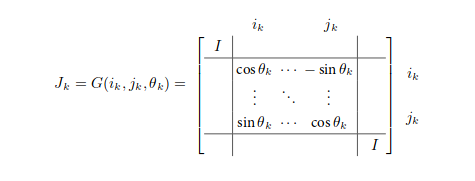
\includegraphics[scale=1]{figurest/figure_1.png}
\end{figure}
\textcolor{blue}{引理}\quad 设$A\in\mathbb{R}^{2\times 2}$是对角矩阵。则存在Givens变换$G\in \mathbb{R}^{2\times 2}$使得$G^TAG$为对角阵。

为了使$A^{(K)}$收敛到一个对角矩阵,其非对角素必须趋向于0。

记$off(A)$为所有非对角元素的平方和,即
$$off(A)=\sum_{i\neq j}a_{ij}^2=\|A^2\|_F^2-\sum_{i=1}^na_{ii}^2$$

我们的目标就是使得$off(A)$尽快趋向于0。

\textcolor{blue}{引理}\quad 设$A=[a_{ij}]_{n\times n}\in \mathbb{R}^{n\times n}$
是对称矩阵。$\widehat{A}=[a_{ij}]_{n\times n}=J^TAJ$,$J=G(i.j,\theta)$,其中
$\theta$的选取使得$\widehat a_{ij}=\widehat a_{ji}=0$,则$$off(\widehat
A)=off(A)-2a_{ij}^2$$
\textcolor{blue}{算法\quad1.1}\quad Jacobi迭代算法
\begin{enumerate}[1:]
	\item Given a symmetric matrix $A\in \mathbb R^{n\times n}$
	\item if eigenvectors are desired then
	\item \quad set $J=I$ and $shift=1$
	\item end if
	\item while not converge do
	\item \quad choose an index pair $(i,j)$such that $a_{ij}\neq 0$
	\item \quad $\tau=(a_{ii}-a_{jj})/(2a-{jj})$
	\item \quad $t=sign(\tau/(|\tau|+\sqrt{1+\tau ^2})$
	\item \quad $c=1/\sqrt{1+t^2},s=c·t$
	\item \quad $A=G(i,j,\theta)^TAG(i,j,\theta)$
	\item \quad if $shift=1$ then 
	\item \qquad $J=J·G(i,j,\theta)$
	\item \quad end if
	\item end while
\end{enumerate}
$a_{ij}$的选取问题

一种直观的选取方法就是使得$a_{ij}$为所有非对角元素中绝对值最大的一个,这就是经典
Jacobi算法。\\
\textcolor{blue}{算法\quad1.2}\quad 经典Jacobi迭代算法
\begin{enumerate}[1:]
	\item Given a symmetric matrix $A\in \mathbb R^{n\times n}$  
	\item if eigenvectors are desired then  
	\item \quad set $J=I$ and $shift=1$  
	\item end if  
	\item while $off(A)>tol $ do
	\item \quad choose $(i,j)$such that $a_{ij}=max_{k\neq l}|a_{kl}|$  
	\item \quad $\tau=(a_{ii}-a_{jj})/(2a-{jj})$  
	\item \quad $t=sign(\tau/(|\tau|+\sqrt{1+\tau ^2})$  
	\item \quad $c=1/\sqrt{1+t^2},s=c·t$  
	\item \quad $A=G(i,j,\theta)^TAG(i,j,\theta)$  
	\item \quad if $shift=1$ then   
	\item \qquad $J=J·G(i,j,\theta)$  
	\item \quad end if  
	\item end while  
\end{enumerate}  
可以证明,经典Jacobi算法至少是线性收敛的。

\textcolor{blue}{定理}\quad 经典Jacobi算法\textcolor{blue}{1.2}是N步局部二次收敛
的,即对足够大的$k$,有$$off(A^{(k+N)})=\mathcal O(off^2(A^{(k)})$$

\textcolor{blue}{循环Jacobi}\quad 经典Jacobi算法的每一步都要寻找绝对值最大的
非对角元,费时不实用。改进:逐行扫描。\\
\textcolor{blue}{算法\quad1.3}\quad 经典Jacobi迭代算法(逐行扫描)
\begin{enumerate}[1:]
	\item Given a symmetric matrix $A\in \mathbb R^{n\times n}$
	\item if eigenvectors are desired then
	\item \quad set $J=I$ and $shift=1$
	\item end if
	\item while $off(A)>tol$ do
	\item \quad for $i=1$ to $n-1$ do
	\item \qquad for$j=i+1$ to $n$ do
	\item \qquad \quad if $a_{ij}\neq 0$ then
	\item \qquad \qquad $\tau=(a_{ii}-a_{jj})/(2a-{jj})$
	\item \qquad \qquad $t=sign(\tau/(|\tau|+\sqrt{1+\tau ^2})$
	\item \qquad \qquad $c=1/\sqrt{1+t^2},s=c·t$
	\item \qquad \qquad $A=G(i,j,\theta)^TAG(i,j,\theta)$
	\item \qquad \qquad if $shift=1$ then
	\item \qquad \qquad \quad$J=J·G(i,j,\theta)$
	\item \qquad \qquad end if
	\item \qquad \quad end if
	\item \qquad end for
	\item \quad end for
	\item end while
\end{enumerate}

循环Jacobi也具有局部二次收敛性。
\subsection{Raylaogh商迭代}
反迭代方法中,以Rayleigh商作为位移。

关于Rayleigh商迭代的收敛性,我们有下面的结论。

\textcolor{blue}{定理}\quad 设$A\in \mathbb R^{n\times n}$对称,且特征值都是单
重的。则当误差足够小时,Rayleigh商迭代中每步迭代所得的正确数字的位数曾至三倍,即
Rayleigh商迭代是局部三次收敛。
\subsection{对称QR迭代}
将带位移的隐式QR方法运用到对称矩阵,就得到对称QR迭代方法。
基础步骤:
\begin{enumerate}[1.]
	\item 对称三对角化:利用Householder变换,将$A$化为对称三对角矩阵,即计算正交
	矩阵$Q$使得$T=QAQ^T$为对称三对角矩阵;
	\item 使用带(单)位移的隐式QR迭代算法计算T的特征值与特征向量;
	\item 计算$A$的特征向量。
\end{enumerate}
对称三对角化

任何一个对称矩阵$A\in \mathbb R^{n\times n}$都可以通过正交变换转化成一个对称三对
角矩阵$T$。这个过程可以通过Householder变换来实现,也可以通过Givens变换来实现。\\
对称QR迭代算法的运算量
\begin{itemize}
	\item[$\bullet$] 三对角化$4n^3/3+\mathcal O(n^2)$,若需计算特征向量,则为
	$8n^3/3+\mathcal O(n^2)$;
	\item[$\bullet$] 对$T$做带位移的隐式QR迭代,每次迭代的运算量为$6n$;
	\item[$\bullet$] 计算特征值,假定每个平均迭代2步,则总运算量为
	$12n^2$;
	\item[$\bullet$] 若要计算$T$的所有特征值和特征向量,则运算量为$6n^3+\mathcal
	O(n^2)$;
	\item[$\bullet$] 若只要计算A的所有特征值,运算量为$4n^3/3+\mathcal O(n^2)$;
	\item[$\bullet$] 若计算$A$的所有特征值和特征向量,则运算量为
	$26n^3/3+\mathcal O(n^2)$;
\end{itemize}

位移的选取——Wilkinson位移

位移的好坏直接影响到算法的收敛速度。我们可以通过下面的方式来选取位移。设
$$A^{(k)}=\begin{bmatrix}
a_1^{(k)}&b_1^{(k)}&&\\
b_1^{(k)}&\ddots &\ddots &\\
&\ddots &\ddots &b_{n-1}^{k}\\
&&b_{n-1}^{(k)}&a_n^{(k)}
\end{bmatrix}$$

一种简单的位移选取策略就是令$\sigma _k=a_n{(K)}$。事实上,$a_n^{(k)}$就是收敛到
特征向量的迭代向量的Rayleigh商。这种位移选取方法几乎对所有的矩阵都有三次渐进收敛速度。但也存在不收敛的例子,故我们需要对其做改进。

\textcolor{blue}{Wilkinson位移:}取$\begin{bmatrix}a_{n-1}^{(k)}&b_{n-1}^{(k)}\\
b_{n-1}^{(k)}&a_n^{(k)} \end{bmatrix}$的最接近$a_n^{(k)}$的特征值作为位移。通过
计算可得Wilkinson位移为
$$\sigma =a_n^{(k)}+\delta -sign(\delta)\sqrt{\delta
	^2+(b_{n-1}^{(k)})^2}$$,
其中$\delta=\
frac{1}{2}(a_{n-1}^{(k)}-a_n^{(K)})$
出于稳定性方面的考虑,我们通常用下面的计算公式\begin{equation}
\sigma=a_n^{(k)}-\cfrac{(b_{n-1}{(k)})^2}{\delta +sign(\delta)\sqrt{\delta
		^2+(b_{n-1}^{(k)})^2}}
\end{equation}

\textcolor{blue}{定理}\quad 采用Wilkinson位移的QR迭代时整体收敛的,且至少是线性收敛。事实上,几乎所有的矩阵都是渐进三次收敛的。

\textcolor{blue}{例}\quad 带Wilkinson位移的隐式QR迭代算法收敛性演示。

MATLAB代码:$Eig_TriQR.m$
\subsection{分而治之法}
分而治之法由Cuppen于1981年首次提出,但直到1995年才出现稳定的实现方式,是目前计算\textcolor{blue}{所有特征值和特征向量}的最快算法。

考虑不可约对称三对角矩阵
$$\begin{aligned}
T&=\left[\begin{array}{cccc|cccc}
a_1&b_1&&&&&&\\
b_1&\ddots & \ddots &&&&&\\
&\ddots &a_{m-1}&b_{m-1}&&&&\\
&&b_{m-1}&a_m&b_m&&&\\
\hline
&&&b_m&a_{m+1}&b_{m+1}&&\\
&&&&b_{m+1}&\ddots&\ddots&\\
&&&&&\ddots&\ddots&b_{n-1}\\
&&&&&&b_{n-1}&a_n
\end{array}\right]\\
&=\left[\begin{array}{cccc|cccc}
a_1&b_1&&&&&&\\
b_1&\ddots & \ddots &&&&&\\
&\ddots &a_{m-1}&b_{m-1}&&&&\\
&&b_{m-1}&a_m-b_m&&&&\\
\hline
&&&&a_{m+1}-b_m&b_{m+1}&&\\
&&&&b_{m+1}&\ddots&\ddots&\\
&&&&&\ddots&\ddots&b_{n-1}\\
&&&&&&b_{n-1}&a_n
\end{array}\right]+\left[\begin{array}{cccc|cccc}
&&&&&&&\\&&&&&&&\\&&&&&&&\\&&&b_m&b_m&&&\\
\hline
&&&b_m&b_m&&&\\&&&&&&&\\&&&&&&&\\&&&&&&&
\end{array}\right]\\
&=\left[\begin{array}{c|c}
T_1&0\\\hline 0&T_1
\end{array}\right]+b_mvv^T
\end{aligned}
$$其中$v=[0,...,0,1,1,0,...,0]^T$。
假定$T_1$和$T_2$的特征值已经计算出来,即$T_1=Q_1\boldsymbol{\Lambda}_1Q_1^T$,$T_2=Q_2\boldsymbol{\Lambda}_2Q_2^T$,下面考虑$T$的特征值分解。
$$
\begin{aligned} T=\left[\begin{array}{cc}{T_{1}} & {0} \\ {0} & {T_{2}}\end{array}\right]+b_{m} v v^{\mathrm{T}} &=\left[\begin{array}{cc}{Q_{1} \Lambda_{1} Q_{1}^{\mathrm{T}}} & {0} \\ {0} & {Q_{2} \Lambda_{2} Q_{2}^{\mathrm{T}}}\end{array}\right]+b_{m} v v^{\mathrm{T}} \\ &=\left[\begin{array}{cc}{Q_{1}} & {0} \\ {0} & {Q_{2}}\end{array}\right]\left(\left[\begin{array}{cc}{\Lambda_{1}} & {0} \\ {0} & {\Lambda_{2}}\end{array}\right]+b_{m} u u^{\mathrm{T}}\right)\left[\begin{array}{cc}{Q_{1}} & {0} \\ {0} & {Q_{2}}\end{array}\right]^{\top} \end{aligned}
$$
其中$$
u=\left[\begin{array}{cc}{Q_{1}} & {0} \\ {0} & {Q_{2}}\end{array}\right]^{\top}
,v=\left[\begin{array}{c}
Q_1^T\mbox{的最后一列}\\Q_2^T\mbox{的第一列}
\end{array}\right]$$

令$a=b_m$,$D=diag(\Lambda_1,\Lambda_2)=diag(d_1,d_2,...,d_n)$,并假定$d_1\ge d_2\ge ...\ge d_n$,则$T$的特征值于$D+\alpha uu^T$的特征值相同。
考虑$D+\alpha uu^T$的特征值

设$\lambda$是$D+\alpha uu^T$的一个特征值,若$D-\lambda I$非奇异,则$$det(D+\alpha uu^T-\lambda I)=det(D-\lambda I)·det(I+\alpha(D-\lambda I)^{-1}uu^T)$$
故$det(D+\alpha uu^T-\lambda I)=0$。

\textcolor{blue}{引理}\quad 设$x,y\in \mathbb R^n$,则$det(I+xy^T)=1+y^Tx$。

于是$$det(I+\alpha(D-\lambda I)^{-1}uu^T)=1+\alpha u^T(D-\lambda I)^{-1}u=1+\alpha \sum_{i=1}^{n}\cfrac{u_i^2}{d_i-\lambda} \triangleq f(\lambda)$$
故求$A$的特征值等价于求特征方程$f(\lambda)=0$的根。\\
由于$$f'(\lambda)=\alpha \sum_{i=1}^{n}\cfrac{u_i^2}{(d_i-\lambda)}$$

当所有的$d_i$都互不相同,且所有的$u_i$都不为零时,$f(\lambda)$在$\lambda \neq d_i$处都是严格单调的。
\begin{figure}[H]
	\centering
	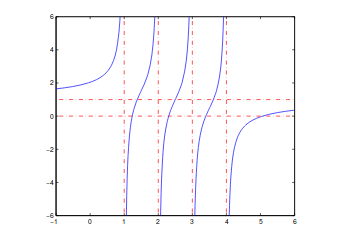
\includegraphics[scale=1]{figurest/figure_2.png}
\end{figure}
所以$f(\lambda)$在每隔区间$(d_{i+1},d_i)$内都有一个根,共$n-1$个,另一个根在$(d_1,\infty)$(若$\alpha >0$)或($-\infty,d_n$)若$\alpha <0$)中。

由于$f(\lambda)$在每个区间$(d_{i+1},d_i)$内光滑且严格单调递增($\alpha >0$)或递减($\alpha <0$),所以在实际计算中,可以使用对分法,牛顿法及其变形,或有理逼近等算法求解。通常都很快收敛,一般只需迭代几步即可。

因此,计算一个特征值的运算量约为$\mathcal{O}(n)$,计算$D+\alpha\ uu^T$的所有特征向量。

\textcolor{blue}{引理}\quad 设$D\in \mathbb R^{n\times n}$为对角矩阵,$u\in \mathbb R^n$,$\alpha \in \mathbb R$,若$\lambda$是$D+\alpha\ uu^T$的特征值,且$\lambda \neq d_i$,$i=1,2,...,n$,则$(D-\lambda I)^{-1}u$是其对应的特征向量。\\
\textcolor{blue}{算法 4.1}\quad 计算对称三对角矩阵的特征值和特征向量的分而治之法
\begin{enumerate}[1:]
	\item function $[Q,\Lambda]=dc\_eig(T)$  \quad $\%T=Q\Lambda Q^T$
	\item if $T$is of $1\times 1$then
	\item \quad $Q=1$,$\Lambda=T$
	\item \quad return
	\item end if
	\item form $T=\left[\begin{array}{cc}{T_{1}} & {0} \\ {0} & {T_{2}}\end{array}\right]+b_{m} v v^{\top}
	$
	\item $\left[Q_{1}, \Lambda_{1}\right]=\mathrm{d} c_{-} \operatorname{eig}\left(T_{1}\right)$
	\item $\left[Q_{2}, \Lambda_{2}\right]=\mathrm{d} c_{-} \operatorname{eig}\left(T_{2}\right)$
	\item form $D+\alpha uu^T$from$\Lambda_{1},\Lambda_{2},Q_1,Q_2$
	\item compute the eigenvalues $\Lambda$and eigenvectors  $\hat{Q}$ of $D+\alpha uu^T$
	\item compute the eigenvalues of $T$ with $Q=\left[\begin{array}{cc}{Q_{1}} & {0} \\ {0} & {Q_{2}}\end{array}\right] \cdot \hat{Q}$
	\item end
\end{enumerate}

在分而治之法中,计算特征值和计算特征向量是同时进行的。

下面我们详细讨论分而治之算法的几个细节问题:
\begin{enumerate}[(1)]
	\item 如何减少运算量;
	\item 如何求解特征方程$f(\lambda)=0$;
	\item 如何稳定的计算特征向量。
\end{enumerate}
(1)如何减小运算量——收缩技巧(deflation)

分而治之算法的计算复杂性分析如下:用$t(n)$表示对$n$阶矩阵调用函数$dc\_eig$的运算量,则
\begin{equation*}
	\begin{aligned}
		t(n)=&2t(n/2)\qquad \mbox{递归调用}dc_eig\mbox{两次}\\&+\mathcal{O}(n^2)\qquad  \mbox{计算}D+\alpha uu^T \mbox{的特征值和特征向量}\\&+c·n^3 \qquad \mbox{计算}Q
	\end{aligned}
\end{equation*}

如果计算$Q$时使用的是稠密矩阵乘法,则$c=2$;若不计$\mathcal{O} (n^2)$项,则由递归公式$t(n)=2t(n/2)+c·n^3$可得$t(n)\thickapprox c·4n^3/3$。

但事实上,由于收缩现象的存在,常熟$c$通常比1小得多。

在前面的算法描述过程中,我们假定$d_i$互不相等且$u_i$不能等于零。

事实上,当$d_i=d_{i+1}$或$u_i=0$时,$d_i$即为$D+\alpha uu^T$的特征值,这种现象我们成为收缩。

在实际计算时,当$d_i-d_{i+1}$或$|u_i|$小于一个给定的阈值时,我们就金斯认为$d_i$为$D+\alpha uu^T$的特征值,即出现收缩现象。

在实际计算中,收缩现象会经常发生,而且会非常频繁,所以我们可以而且应该利用这种有点加快分而治之算法的速度。

由于主要的计算量集中在计算$Q$,即算法的最后一步的矩阵的乘积。如果$u_i=0$,则$d_i$为特征值,其对应的特征向量$e_i$,即$\hat{Q}$的第$i$列为$e_i$,故计算$Q$的第$i$列时不需要做任何的计算。

当$d_i=d_{i+1}$时,也存在一个类似的简化。\\
(2)特征方程求解

通常我们可以使用牛顿法来计算特征方程$f(\lambda)=0$的解。当$d_i\neq d_{i+1}$且$u_i\neq 0$时,用牛顿法计算$f(\lambda)$在$(d_{i+1},d_i)$中的零点$\lambda _i$。如果$|u_i|$小于给定的阈值时,我们可直接将$d_i$作为特征值$\lambda _i$的一个近似。但当$u_i$很小(却大于给定的阈值)时,此时$f(\lambda)$在区间$[d_{i+1},d_i]$中的大部分处的斜率几乎为0(见下图)。这是,如果任取$[d_{i+1},d_i]$中的一个点作为迭代初始点,经过一次牛顿迭代后,迭代解可能会跑到区间$[d_{i+1},d_i]$的外面,造成不收敛。
\begin{figure}[H]
	\centering
	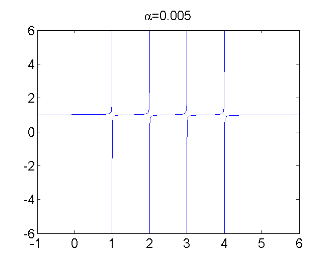
\includegraphics[scale=1]{figurest/figure_3.png}
	\caption{$f(\lambda)=1+0.005(\cfrac{1}{4-\lambda}+\cfrac{1}{3-\lambda}+\cfrac{1}{2-\lambda}+\cfrac{1}{1-\lambda})$的图像}
\end{figure}

这时需要采用修正的牛顿法。假设我们已经计算出$\lambda _i$的一个近似$\tilde{\lambda}$,下面我们需要从$\tilde{\lambda}$出发,利用牛顿迭代计算下一个近似,直至收敛。我们知道牛顿法的基本原理是使用$f(\lambda)$在点$\tilde{\lambda}$的切线来近似$f(\lambda)$,并将切线的零点作为下一个近似,即用直线来近似曲线$f(\lambda)$。

当$u_i$很小时,这种近似方法会出现问题,此时不能使用直线来近似$f(\lambda)$。这时我们可以寻找其他简单函数$h(\lambda)$来近似$f(\lambda)$,然后用$h(\lambda)$的零点作为$f(\lambda)$零点的近似,并不断迭代下去,直至收敛。

当然,$h(\lambda)$需要满足一定的要求:
\begin{enumerate}[(1)]
	\item 必须容易构造;
	\item 其零点容易计算;
	\item 尽可能与$f(\lambda)$相近。
\end{enumerate}

下面给出构造$h(\lambda)$的一种方法。

因为$d_i$和$d_{i+1}$是$f(\lambda)$的奇点,所以我们令$$h(\lambda)=\cfrac{c_1}{d_i-\lambda}+\cfrac{c_2}{d_{i+1}-\lambda}+c_3$$
其中$c_1,c_2,c_3$为参数。显然,$h(\lambda)$的零点很容易计算(与Newton法相差无几)。在选取这些参数时,要使得$h(\lambda)$在$\tilde{\lambda}$附近尽可能地接近$f(\lambda)$。记$$\begin{aligned}
f(\lambda)=1+\alpha \sum_{k=1}^n \cfrac{u_k^2}{d_k-\lambda}&=1+\alpha (\sum_{k=1}^i \cfrac{u_k^2}{d_k-\lambda}+1+\alpha \sum_{k=i+1}^n \cfrac{u_k^2}{d_k-\lambda})\\&\triangleq 1+\alpha\left(\Psi_{1}(\lambda)+\Psi_{2}(\lambda)\right)
\end{aligned}$$

当$\lambda \in (d_{i+1},d_i)$时,$\Psi_{1}(\lambda)$为正项和,$\Psi_{2}(\lambda)$为负项的和,因此它们都可以较精确地计算。但如果把它们加在一起时可能会引起对消,从而失去相对精度。因此我们也将$h(\lambda)$写成$$h(\lambda)=1+\alpha(h_1(\lambda)+h_2(\lambda))$$
其中$$
h_{1}(\lambda)=\frac{c_{1}}{d_{i}-\lambda}+\hat{c}_{1}, \quad h_{2}(\lambda)=\frac{c_{2}}{d_{i+1}-\lambda}+\hat{c}_{2}
$$
满足$$
\begin{aligned} h_{1}(\tilde{\lambda}) &=\Psi_{1}(\tilde{\lambda}), \quad h_{1}^{\prime}(\tilde{\lambda})=\Psi_{1}^{\prime}(\tilde{\lambda}) \\ h_{2}(\tilde{\lambda}) &=\Psi_{2}(\tilde{\lambda}), \quad h_{2}^{\prime}(\tilde{\lambda})=\Psi_{2}^{\prime}(\tilde{\lambda}) \end{aligned}
$$
即$h_{1}(\lambda)$和$h_{2}(\lambda)$分别在点$\tilde{\lambda}$与$\Psi_{1}(\lambda)$和$\Psi_{2}(\lambda)$相切。这在数值插值中是常见的条件。容易计算可得\begin{equation}
\left\{\begin{array}{ll}{c_{1}=\Psi_{1}^{\prime}(\tilde{\lambda})\left(d_{i}-\tilde{\lambda}\right)^{2},} & {\hat{c}_{1}=\Psi_{1}(\tilde{\lambda})-\Psi_{1}^{\prime}(\tilde{\lambda})\left(d_{i}-\tilde{\lambda}\right)} \\ {c_{2}=\Psi_{2}^{\prime}(\tilde{\lambda})\left(d_{i+1}-\tilde{\lambda}\right)^{2},} & {\hat{c}_{2}=\Psi_{2}(\tilde{\lambda})-\Psi_{2}^{\prime}(\tilde{\lambda})\left(d_{i+1}-\tilde{\lambda}\right)}\end{array}\right.
\label{equation5.3}
\end{equation}
所以,最后取\begin{equation}
h(\lambda)=1+\alpha\left(\hat{c}_{1}+\hat{c}_{2}\right)+\alpha\left(\frac{c_{1}}{d_{i}-\lambda}+\frac{c_{2}}{d_{i+1}-\lambda}\right)
\label{equation5.4}
\end{equation}
这就是迭代函数。
\textcolor{blue}{算法 4.2}\quad 修正的Newton算法
\begin{enumerate}[1:]
	\item set$k=0$
	\item choose an initial guess $\lambda _0\in [d_{i+1},d_i]$
	\item while not convergence do
	\item \quad let$\tilde{\lambda}=\lambda _k$and compute $c_1,c_2,\hat{c}_{1},\hat{c}_{2}$from \ref{equation5.3}
	\item \quad set $k=k+1$
	\item \quad compute the solution $\lambda _k$of $h(\lambda)$defined by \ref{equation5.4}
	\item end while
\end{enumerate}
(3)计算特征向量的稳定算法

设$\lambda_i$是$D+\alpha uu^T$的特征值,则根据引理4.2,可利用公式$\left(D-\lambda_{i} I\right)^{-1} u$来计算其对应的特征向量。但遗憾的是,当相邻的两个特征值非常接近时,这个公式可能不稳定。即当$\lambda_i$与$\lambda_{i+1}$非常接近时,他们都靠近$d_{i+1}$(这里假定$\lambda_{i} \in\left(d_{i+1}, d_{i}\right)$),在计算$d_{i+1}-\lambda_{i}$和$d_{i+1}-\lambda_{i+1}$时会存在对消,这就可能损失有效数字,产生较大的相对误差,从而导致$\left(D-\lambda_{i} I\right)^{-1} u$与$\left(D-\lambda_{i+1} I\right)^{-1} u$的计算时不准确的,正交性也会失去。下面的定理可以解决这个问题。

\textcolor{blue}{定理(Löwner)}\quad 设对角阵$D=\operatorname{diag}\left(d_{1}, d_{2}, \dots, d_{n}\right)$满足$d_{1}>d_{2}>\cdots>d_n$,若矩阵$\hat{D}=D+\hat{u} \hat{u}^{\top}$的特征值
$\lambda_{1}, \lambda_{2}, \ldots, \lambda_{n}$满足交错性质\begin{equation}
\lambda_{1}>d_{1}>\lambda_{2}>d_{2}>\cdots>\lambda_{n}>d_{n}
\label{equation5.5}
\end{equation}
则向量$\hat{u}$的分量满足\begin{equation}
\left|\hat{u}_{i}\right|=\left(\frac{\prod_{k=1}^{n}\left(\lambda_{k}-d_{i}\right)}{\prod_{k=1, k \neq i}^{n}\left(d_{k}-d_{i}\right)}\right)^{1 / 2}
\label{equation5.6}
\end{equation}
因此,我们可以采用公式\ref{equation5.6}来计算特征向量。这样就尽可能的避免了出现分母很小的情形。\\
箭型分而治之法

分而治之算法于1981年被首次提出,但直到1995年才由Gu和Eisenstat给出了一种快速稳定的实现方式,称为\textcolor{blue}{箭型分而治之法(Arrowhead Divide-and-Conquer}, ADC).他们做了大量的数值试验,在试验中,当矩阵规模不超过6时,就采用对称QR迭代来计算特征值和特征向量。在对特征方程求解时,他们采用的是修正的有理逼近法。数值结果表明, ADC算法的计算精度可以与其他算法媲美,而计算速度通常比对称QR迭代快5至10倍,比Cuppen的分而治之法快2倍。详细介绍参见相关文献。
\subsection{对分法和逆迭代}
对分法的基本思想是利用惯性定理来计算所需的部分特征值。

\textcolor{blue}{定义}\quad 设$A$为对称矩阵,则其惯性定义为$$
(A)=(\nu, \zeta, \pi)
$$
其中$\nu, \zeta, \pi$分别表示$A$的负特征值,零特征值和正特征值的个数。

\textcolor{blue}{定理(Sylvester惯性定理)}\quad 设$A \in \mathbb{R}^{n \times n}$是对称矩阵,$X \in \mathbb{R}^{n \times n}$非奇异,则$X^TAX$与$A$有相同的惯性。

利用LU分解可得$A-z I=L D L^{\top}$,其中$L$为奇异下三角矩阵,$D$为对角阵,则$$
(A-z I)=\text { Inertia }(D)
$$
由于$D$时对角矩阵,所以$\text { Inertia }(D)$很容易计算。

设$\alpha \in \mathbb{R}^{n}$,记Negcount$(A,\alpha)$为小于$\alpha$的$A$的特征值的个数,即$$
\operatorname{Negcount}(A, \alpha)=\#(\lambda(A)<\alpha)
$$

设$\alpha_{1}<\alpha_{2}$,则$A$在区间$\left[\alpha_{1}, \alpha_{2}\right)$中的特征值个数为$$
\left(A, \alpha_{2}\right)-\operatorname{Negcount}\left(A, \alpha_{1}\right)
$$。

如果$\alpha_{2}-\alpha_{1}<t o l$(其中$tol\ll 1$为事先给定的阈值),且$A$在$\left[\alpha_{1}, \alpha_{2}\right)$中有特征值,则我们可将$\left[\alpha_{1}, \alpha_{2}\right)$中的任意一个值作为$A$在该区间中的特征值的近似。

由此我们可以给出下面的对分法。\\
\textcolor{blue}{算法 5.1}\quad 计算$A$在$\left[a, b\right)$中的所有特征值
\begin{enumerate}[1:]
	\item Let $tol$be a given threshold
	\item compute $n_a=$Negcount $(A, a)$
	\item compute $n_b=$Negcount $(A, b)$
	\item if $n_a=n_b$then
	\item \quad return\qquad \%此时$[a,b)$中没有$A$的特征值
	\item end if
	\item put $\left(a, n_{a}, b, n_{b}\right)$onto worklist
	\item \quad \%worklist 中的元素时“四元素对
	,即由四个数组成的数对
	\item while worklist not empty do
	\item \quad remove$\left(l o w, n_{l o w}, u p, n_{u p}\right)$from the worklist
	\item \quad \%$\left(l o w, n_{l o w}, u p, n_{u p}\right)$是worklisth中的任意一个元素
	\item \quad if$(up-low)<tol$ then
	\item \qquad print ”There are $n_{up}-n_{low}$eigenvalues in[low,up)"
	\item \quad else
	\item \qquad compute $mid=(low+up)/2$
	\item \qquad compute$n_{m i d}=$ Negcount $(A, m i d)$
	\item \qquad if $\left(n_{m i d}>n_{l o w}\right)$ then
	\item \qquad \quad put $\left(l o w, n_{l o w}, m i d, n_{m i d}\right)$onto worklist
	\item \qquad end if
	\item \qquad if $\left(n_{up}>n_{mid}\right)$ then
	\item \qquad \quad $\left(m i d, n_{m i d}, u p, n_{u p}\right)$onto worklist
	\item \qquad end if
	\item \quad end if
	\item end while
\end{enumerate}

对分法的主要运算量集中在计算Negcount $(A, z)$。通常是事先将$A$转化成对称三对角矩阵,这样计算$A-z I$的$\mathrm{LDL}^{\mathrm{T}}$分解就非常简单:
\begin{equation*}
	\begin{aligned}
		A-z I&=\left[\begin{array}{cccc}{a_{1}-z} & {b_{1}} & {} & {} \\ {b_{1}} & {\ddots} & {\ddots} & {} \\ {} & {\ddots} & {\ddots} & {b_{n-1}} \\ {} & {} & {b_{n-1}} & {a_{n}-z}\end{array}\right]
		\\
		&=\left[\begin{array}{cccc}{1} \\ {l_{1}} & {\ddots} & {} & {} \\ {} & {\ddots} & {\ddots} & {} \\ {} & {} & {l_{n-1}} & {1}\end{array}\right]\left[\begin{array}{cccc}{d_{1}} & {} & {}&  \\ {} & {\ddots} & {} & {} \\ {}  & {} & {\ddots} & {} \\ {} & {} & {}  & {d_{n}}\end{array}\right] \left[\begin{array}{cccc}{1} & {l_{1}} & {} & {} \\ {} & {\ddots} & {\ddots} & {}  \\ {} & {} & {\ddots} & {l_{n-1}} \\ {} & {} & {} & {1}\end{array}\right] \triangleq L D L^{\top}
	\end{aligned}
\end{equation*}

利用待定系数法,可以得到下面的递推公式
\begin{equation}
d_{1}=a_{1}-z, \quad d_{i}=\left(a_{i}-z\right)-\frac{b_{i-1}^{2}}{d_{i-1}}, \quad i=2,3, \ldots, n
\label{equation5.7}
\end{equation}

用上面的公式计算$d_i$的运算量约为$4n$。

注意这里没有选主元,但针对对称三对角矩阵,该算法是非常稳定的,即使当$d_i$有可能很小时,算法依然很稳定。

\textcolor{blue}{定理[Demmel ’97]}利用公式\ref{equation5.7}计算所得的$d_i$与精确计算$\hat{A}$的$\hat{d}_i$有相同的符号,故有相同的惯性。这里$\hat{A}$与$A$非常接近,即$$
\hat{A}(i, i)=a_{i}, \quad \hat{A}(i, i+1)=b_{i}\left(1+\varepsilon_{i}\right)
$$
其中,$\left|\varepsilon_{i}\right| \leq 2.5 \varepsilon+O\left(\varepsilon^{2}\right)$,这里
$\varepsilon$为机器精度。
\begin{itemize}
	\item 由于单独调用一次Negcount的运算量为$4n$,故计算$k$个特征值的总运算量约为$O(k n)$;
	\item 当当特征值计算出来后,我们可以使用带位移的逆迭代来计算对应的特征向量。通常只需迭代1至2次即可,由于$A$是三对角矩阵,故计算每个特征向量的运算量为$O(n)$;
	\item 当特征值紧靠在一起时,计算出来的特征向量可能会失去正交性,此时需要进行再正交化,可通过MGS的QR分解来实现。
\end{itemize}
\subsection{奇异值分解}
奇异值分解(SVD)具有十分广泛的应用背景,因此,如何更好更快地计算一个给定矩阵的SVD是科学与工程计算领域中的一个热门研究课题,吸引了众多专家进行这方面的研究,也涌现出了许多奇妙的方法.本章主要介绍计算SVD的常用算法。

对任意矩阵$A \in \mathbb{R}^{m \times n}$,其奇异值与对称矩阵$A^TA$,$AA^T$和$\left[\begin{array}{ll}{0} & {A^{\top}} \\ {A} & {0}\end{array}\right]$的特征值是密切相关的,故理论上计算对称特征值的算法都可以用于计算奇异值。但在实际计算中,我们通过可以利用SVD的特殊结构使得算法更加有效和准确。

与计算对称矩阵的特征值累死,计算一个矩阵A的奇异值分解的算法通常分为一下几个步骤(Jacobi算法除外):
\begin{enumerate}[1.]
	\item 将$A$二对角化:$B=U_1^TAV_1$,其中$B$为上二对角矩阵,$U_1,V_1$为正交阵;
	\item 计算$B$的SVD:$B=U_2\sum V_2^T$,其中$\sum$为对角阵,$U_2,V_2$为正交阵;
	\item 合并得到$A$的SVD:$A=U_1BV_1^T=(U_1U_2)B(V_1V_2)^T$。
\end{enumerate}
\subsubsection{二对角化}
我们知道。对称矩阵可以通过一系列Householder变换转化为对称三对角矩阵。对于一般矩阵$A \in \mathbb{R}^{m \times n}$,我们也可以通过Householder变换,将其转化为而对角矩阵,即计算正交矩阵$U_1$和$V_1$使得
\begin{equation}
U_1^TAV_1=B
\label{equation5.8}
\end{equation}
其中$B$是一个实(上)二对角矩阵。这个过程就称为\textcolor{blue}{二对角化}。

需要注意的是,与对称矩阵的对称三对角化不同,$A$与$B$是不相似的。

设$A \in \mathbb{R}^{m \times n}$,二对角化过程大致如下:
\begin{enumerate}[(1)]
	\item 首先确定一个Household矩阵$H_1 \in \mathbb{R}^{m \times n}$,使得$H_1A$的第一节除第一个元素外,其他分量都为零,即$$H_1A=\left[\begin{array}{ccccc}{*} & {*} & {*} & {*} & {*} \\ {0} & {*} & {*} & {\cdots} & {*} \\ {0} & {*} & {*} & {\cdots} & {*} \\ {0} & {*} & {*} & {\cdots} & {*} \\ {\vdots} & {\vdots} & {\vdots} & {} & {\vdots} \\ {0} & {*} & {*} & {\cdots} & {*}\end{array}\right]$$
	\item 再确定一个Household矩阵$\tilde{H}_{1} \in \mathbb{R}^{(n-1) \times(n-1)}$,把$H_1A$的第一行的第$3$至第$n$个元素化为零,即$$
	H_{1} A\left[\begin{array}{cc}{1} & {0} \\ {0} & {\tilde{H}_{1}}\end{array}\right]=\left[\begin{array}{ccccc}{*} & {*} & {0} & {\cdots} & {0} \\ {0} & {*} & {\cdots} & {*} \\ {0} & {*} & {\cdots} & {*} \\ {0} & {*} & {\cdots} & {*} \\ {\vdots} & {\vdots} & {} & {\vdots} \\ {0} & {*} & {\cdots} & {*}\end{array}\right]
	$$
	\item 重复上面的过程,直到把$A$最终化为而对角矩阵。
\end{enumerate}

有了分解\ref{equation5.8}以后,我们可得$$
A^{\top} A=\left(U_{1} B V_{1}^{\top}\right)^{\top} U_{1} B V_{1}^{\top}=V_{1} B^{\top} B V_{1}^{\top}
$$即$V_{1}^{\top} A^{\top} A V_{1}=B^{\top} B$。由于$B^TB$是对称三对角的,所以这就相当于将$A^TA$三对角化。

整个二对角化过程的运算量约为$4mn^2+4m^2n-4n^3/3$。若不需要计算$U_1$和$V_1$,则运算量约为$4mn^2-4n^3/3$。\\
二对角矩阵的奇异值分解

设$B \in \mathbb{R}^{n \times n}$是一个而对角矩阵$B=\left[\begin{array}{cccccc}{a_{1}} & {b_{1}} & {} & {} & {} \\ {} & {\ddots} & {\ddots} & {} \\ {} & {} & {\ddots} & {} & {} \\ {} & {} & {\ddots} & {b_{n-1}} \\ {} & {} & {} & {a_{n}}\end{array}\right]$,则下面三种方法均可将计算$B$的SVD转化成计算对称三对角矩阵的特征分解:
\begin{enumerate}[(1)]
	\item 令$A=\left[\begin{array}{ll}{0} & {B^{\top}} \\ {B} & {0}\end{array}\right]$,置换阵$P=\left[e_{1}, e_{n+1}, e_{2}, e_{n+2}, \ldots, e_{n}, e_{2 n}\right]$,则$T_{p s}=P^{\top} A P$是对称三对角矩阵,且$T_{p s}$的主对角线元素全为0,次对角线元素为$a_{1}, b_{1}, a_{2}, b_{2}, \dots, a_{n-1}, b_{n-1}, a_{n}$。若$\left(\lambda_{i}, x_{i}\right)$是$T_{p s}$的一个特征对,则$$
	\lambda_{i}=\pm \sigma_{i}, \quad P x_{i}=\frac{1}{\sqrt{2}}\left[\begin{array}{c}{v_{i}} \\ { \pm u_{i}}\end{array}\right]
	$$,其中$\sigma_{i}$为$B$一个奇异值,$u_i$和$v_i$分别为对应的左和右奇异向量。
	\item 令$T_{B B^{\top}}=B B^{\prime}$,则$$
	T_{B B^{\top}}=\left[\begin{array}{cccc}{a_{1}^{2}+b_{1}^{2} a_{2} b_{1}} & {} & {} \\ {a_{2} b_{1}} & {\ddots} & {\ddots} & {} \\ {} & {\ddots} & {a_{n-1}^{2}+b_{n-1}^{2} a_{n} b_{n-1}} \\ {} & {} & {a_{n} b_{n-1}} & {a_{n}^{2}}\end{array}\right]
	$$
	$T_{B B^{\top}}$的特征值为$B$的奇异值的平方,且$T_{B B^{\top}}$的特征向量为$B$的左奇异向量。
	\item 令$T_{B B^{\top}}=B B^{\prime}$,则$$
	T_{B^{\top} B}=\left[\begin{array}{cccc}{a_{1}^{2}} & {a_{1} b_{1}} \\ {a_{1} b_{1}} & {a_{2}^{2}+b_{1}^{2}} & {\ddots} \\ {} & {\ddots} & {\ddots} & {a_{n-1} b_{n-1}} \\ {} & {} & {a_{n-1} b_{n-1}} & {a_{n}^{2}+b_{n-1}^{2}}\end{array}\right]
	$$
	$T_{B^{\top} B}$的特征值为$B$的奇异值的平方,且$T_{B^{\top} B}$的特征向量为$B$的右奇异向量。
\end{enumerate}

理论上,我们可以直接使用QR迭代、分而治之法或带反迭代的对分法,计算三对角矩阵的$T_{p s}, T_{B B^{\top}}$和$T_{B^{\top} B}$的特征值和特征向量。但一般来说,这种做法并不是最佳的,原因如下:
\begin{enumerate}[(1)]
	\item 对$T_{p s}$做QR迭代并不划算,因为QR迭代计算所有的特征值和特征向量,而事实上只要计算正的特征值即可;
	\item 直接构成$T_{B B^{\top}}$或$T_{B^{\top} B}$是数值不稳定的。事实上,这样做可能会使得$B$的小奇异值的精度丢失一半。
\end{enumerate}

下面是一些奇异值分解的比较实用的算法。
\begin{enumerate}[1.]
	\item \textcolor{blue}{Golub-Kahan SVD算法}:由Golub和Kahan于1965年提出,是一种十分稳定且高效的计算SVD的算法。主要思想是将带位移的对称QR迭代算法隐式地用到$B^TB$上,在该算法中,并不需要显示地把$B^TB$计算出来。该算法也通常就称为SVD算法,是一个基本且实用的算法,目前仍然是计算小规模矩阵奇异值分解的常用算法。
	\item \textcolor{blue}{dqds算法}:由Fernando和Parlett于1994年提出,是计算二对角矩阵所有奇异值的最快算法,而且能达到很高的相对精度,包括奇异值很小的情形。该算法主要基于对$B^TB$的Cholesky迭代,可以看作是LR迭代算法的改进。由于LR迭代算法在一定条件下与对称QR算法是等价的,因此该算法也可以看作是QR迭代的变形。
	\item \textcolor{blue}{分而治之法}:该算法是计算维数$n \geq 25$的矩阵的所有奇异值和奇异向量的最快算法,但不能保证小奇异值的相对精度,即$\sigma_{i}$的相对精度为$O(\varepsilon) \sigma_{1}$,而不是$O(\varepsilon) \sigma_{i}$。
	\item \textcolor{blue}{对分法和反迭代}:主要用于计算某个区间内的奇异值及对应的奇异向量,能保证较高的相对精度。
	\item \textcolor{blue}{Jacobi迭代}:可隐式地对$AA^T$或$A^TA$实施对称Jacobi迭代,能保证较高的相对精度。最近,Z.Drmac和K.Veselić改进了最初的Jacobi算法,使其变成一个速度快、精度高的实用算法。
\end{enumerate}

在这里,我们简要介绍Golub-Kahan SVD算法, dqds算法和Jacobi迭代。
\subsubsection{Golub-Kahan SVD算法}
该算法主要思想是将带位移的对称QR迭代算法隐式地用到$B^TB$上,而无需将$B^TB$显示的计算出来。\\
算法基本框架

Golub-Kahan SVD算法有时也简称SVD算法,其基本框架是:
\begin{itemize}
	\item 将矩阵$A$二对角化,得到上二对角矩阵$B$;
	\item 用隐式QR迭代计算$B^TB$的特征值分解,即
	\begin{equation}
	B^{\top} B=Q \Lambda Q^{\top}, \quad \Lambda=\operatorname{diag}\left(\sigma_{1}^{2}, \sigma_{2}^{2}, \ldots, \sigma_{n}^{2}\right)
	\label{equation5.9}
	\end{equation}
	\item 计算$BQ$的列主元QR分解,即\begin{equation}
	(B Q) P=U R
	\label{equation5.10}
	\end{equation}
	其中$P$是置换矩阵,$U$是正交矩阵,$R$是上三角矩阵。
\end{itemize}

由\ref{equation5.9}可知$$
(B Q)^{\top} B Q=\Lambda
$$
因此$BQ$是列正交矩阵(但不是单位列正交)。再由\ref{equation5.10}可知$R=U^T(BQ)P$也是列正交矩阵。又$R$是上三角矩阵,所以$R$必定是对角矩阵。令$V=QP$,则由\ref{equation5.10}可知$$U^TBV=R$$这就是二对角矩阵$B$的奇异值分解。

\textcolor{blue}{算法的具体实现参见相关文献}
\subsubsection{dqds算法}
我们首先介绍针对实对称正定矩阵的LR算法,该算法思想与QR迭代算法类似,但提出时间更早。\\
\textcolor{blue}{算法 6.1}\quad 带位移的LR算法
\begin{enumerate}[1:]
	\item Let $T_0$ be a given real symmetric positive definite matrix
	\item set $i=0$
	\item while not converge do 
	\item \quad choose a shift$\tau_{i}^{2}$ satisfying $\tau_{i}^{2}<\min \left\{\lambda\left(T_{i}\right)\right\}$
	\item \quad compute $B_i$ such that $T_{i}-\tau_{i}^{2} I=B_{i}^{\top} B_{i}$\qquad \%Cholesky factorization
	\item \quad $T_{i+1}=B_{i} B_{i}^{\top}+\tau_{i}^{2} I$
	\item \quad $i=i+1$
	\item end while
\end{enumerate}

LR迭代算法在形式上与QR迭代算法非常类似。事实上,对于不带位移的LR迭代算法,我可以证明,两步LR迭代等价于一步QR迭代。

\textcolor{blue}{引理}\quad 设$\tilde{T}$是不带位移的LR算法迭代两步后生成的矩阵,$\hat{T}$是不带唯一的QR算法迭代一步后生成的矩阵,则$\tilde{T}=\hat{T}$。

\begin{enumerate}[(1)]
	\item LR算法中要求$T_0$对称正定,但并不一定是三对角矩阵;
	\item 由该引理可知,QR算法与LR算法有相同的收敛性。
\end{enumerate}
dqds算法

该算法是针对三对角的对称正定矩阵$B^TB$,其中$B$是而对角矩阵。在数学上, dqds算法与LR算法是等价的,但在该算法中,我们是直接通过$B_i$来计算$B_{i+1}$,从而避免计算中间矩阵$T_{i+1}$,这样也就尽可能的避免了由于计算$B_iB_i^T$而可能带来的数值不稳定性。

下面推导如何从$B_i$直接计算$B_{i+1}$。设
$$
B_{i}=\left[\begin{array}{cccc}{a_{1}} & {b_{1}} & {} & {} \\ {} & {a_{2}} & {\ddots} & {} \\ {} & {} & {\ddots} & {b_{n-1}} \\ {} & {} & {} & {a_{n}}\end{array}\right], \quad B_{i+1}=\left[\begin{array}{cccc}{\tilde{a}_{1} \tilde{b}_{1}} \\ {\tilde{a}_{2} \ddots} \\ {\ddots} & {\tilde{b}_{n-1}} \\ {\tilde{a}_{n}}\end{array}\right]
$$

为了书写方便,我们记$b_{0}=b_{n}=\tilde{b}_{0}=\tilde{b}_{n}=0$。由LR算法6.1可知
$$
B_{i+1}^{\top} B_{i+1}+\tau_{i+1}^{2} I=B_{i} B_{i}^{\top}+\tau_{i}^{2} I
$$
比较等式两边矩阵的对角线和上对角线元素,可得
$$
\tilde{a}_{k}^{2}+\tilde{b}_{k-1}^{2}+\tau_{i+1}^{2}=a_{k}^{2}+b_{k}^{2}+\tau_{i}^{2}, \quad k=1,2, \ldots, n
$$

$$
\tilde{a}_{k} \tilde{b}_{k}=a_{k+1} b_{k} \quad \text {或} \quad \tilde{a}_{k}^{2} \tilde{b}_{k}^{2}=a_{k+1}^{2} b_{k}^{2}, \quad k=1,2, \ldots, n-1
$$
记$\delta=\tau_{i+1}^{2}-\tau_{i}^{2}, p_{k}=a_{k}^{2}, q_{k}=b_{k}^{2}, \tilde{p}_{k}=\tilde{a}_{k}^{2}, \tilde{q}_{k}=\tilde{b}_{k}^{2}$,则可得qds算法:\\
\textcolor{blue}{算法 6.2}\quad qds算法的单步$\left(B_{i} \rightarrow B_{i+1}\right)$
\begin{enumerate}[1:]
	\item $\delta=\tau_{i+1}^{2}-\tau_{i}^{2}$
	\item for $k=1$ to $n-1$ do
	\item \quad $\tilde{p}_{k}=p_{k}+q_{k}-\tilde{q}_{k-1}-\delta$
	\item $\tilde{q}_{k}=q_{k} \cdot\left(p_{k+1} / \tilde{p}_{k}\right)$
	\item end for 
	\item $\tilde{p}_{n}=p_{n}-\tilde{q}_{n-1}-\delta$
\end{enumerate}

qds算法中的每个循环仅需5个浮点运算,所以运算量较少。

为了体验算法的精确性,我们引入一个辅助变量$d_{k} \triangleq p_{k}-\tilde{q}_{k-1}-\delta$,则
$$
\begin{aligned} d_{k} &=p_{k}-\tilde{q}_{k-1}-\delta \\ &=p_{k}-\frac{q_{k-1} p_{k}}{\tilde{p}_{k-1}}-\delta \\ &=p_{k} \cdot \frac{\tilde{p}_{k-1}-q_{k-1}}{\tilde{p}_{k-1}}-\delta \\ &=p_{k} \cdot \frac{p_{k-1}-\tilde{q}_{k-2}-\delta}{\tilde{p}_{k-1}}-\delta \\ &=\frac{p_{k}}{\tilde{p}_{k-1}} \cdot d_{k-1}-\delta \end{aligned}
$$

于是就可得到dqds算法。
\textcolor{blue}{算法 6.3}\quad dqds算法的单步$\left(B_{i} \rightarrow B_{i+1}\right)$
\begin{enumerate}[1:]
	\item $\delta=\tau_{i+1}^{2}-\tau_{i}^{2}$
	\item $d_{1}=p_{1}-\delta$
	\item for $k=1$ to $n-1$ do
	\item \quad $\tilde{p}_{k}=d_{k}+q_{k}$
	\item \quad $t=p_{k+1} / \tilde{p}_{k}$
	\item \quad $\tilde{q}_{j}=q_{k} \cdot t$
	\item \quad $d_{k+1}=d_{k} \cdot t-\delta$
	\item end for 
	\item $\tilde{p}_{n}=d_{n}$
\end{enumerate}

dqds算法的运算量与dqs差不多,但更精确。

下面的定理显示了dqds算法的高精度性质。

\textcolor{blue}{定理}\quad 以浮点运算对$B$做单步dqds迭代,得到矩阵$\tilde{B}$,该过程等价于
\begin{enumerate}[1.]
	\item 对$B$的每个元素座椅而小德相对扰动(不超过$1.5\varepsilon$),得到$\tilde{B}$;
	\item 对$\tilde{B}$应用精确的dqds算法的单步,得到$\overline{B}$;
	\item 对$\overline{B}$的每个元素做一个小的相对扰动(不超过$\varepsilon$),得到$\tilde{B}$。
\end{enumerate}

因此,$B$和$\tilde{B}$的奇异值满足高的相对精度。

关于dqds算法中位移的选取,以及如何判断收敛性,可以参见相关文献。
\subsubsection{Jacobi算法}
本节讨论对矩阵$M=A^TA$实施隐式的Jacoi算法来计算$A$的奇异值。

我们知道,Jacobi算法的每一步就是对矩阵作Jacobi旋转,即$A^TA\rightarrow J^TA^TAJ$,其中$J$的选取将两个非对角元化为0。在实际计算中,我们只需计算$AJ$,故该算法称为\textcolor{blue}{单边Jacobi旋转}。\\
\textcolor{blue}{算法 6.4}\quad 单边Jacobi旋转的单步

\%对$M=A^TA$作Jacobi旋转,将$M(i.j),M(j,i)$化为0
\begin{enumerate}[1:]
	\item Compute $m_{ii}=(A^TA)_{ii},m_{ij}=(A^TA)_{ij},m_{jj}=(A^TA)_{jj}$
	\item if $m_{ij}$ is not small enough then 
	\item \quad $\tau=\left(m_{i i}-m_{j j}\right) / \left(2 \cdot m_{i j}\right)$
	\item \quad $t=\operatorname{sign}(\tau) /\left(|\tau|+\sqrt{1+\tau^{2}}\right)$
	\item \quad $c=1 / \sqrt{1+t^{2}}$
	\item \quad $s=c·t$
	\item \quad $A=A G(i, j, \theta)$ \qquad \% $G(i,j,\theta)$为Givens变换
	\item \quad if eigenvectors are desired then
	\item \qquad $J=J·G(i, j, \theta)$
	\item \quad end if
	\item end if
\end{enumerate}

在上面算法的基础上,我们可以给出完整的单边Jacobi算法。
\text{blue}{算法 6.5}\quad 单边Jacobi算法:计算$A=U\sum V^T$
\begin{enumerate}[1:]
	\item while $A^TA$ is not diagonal enough do
	\item \quad for $i=1$ to $n-1$do
	\item \qquad for $j=i+1$to $n$ do
	\item \qquad \quad 调用单边Jacobi旋转
	\item \qquad end for 
	\item \quad end for 
	\item end while 
	\item compute $\sigma_{i}=\|A( :, i)\|_{2}, i=1,2, \ldots n$
	\item $U=\left[u_{1}, \dots, u_{n}\right]$with $u_{i}=A( :, i) / \sigma_{i}$
	\item $V=J$
\end{enumerate}

Jacobi算法的特点
\begin{itemize}
	\item 不需要双对角化,这样可以避免双对角化引入的误差;
	\item 可以达到相对较高的计算精度;
	\item 速度较慢。(目前已有快速的改进算法)
\end{itemize}

\textcolor{blue}{定理}\quad 设$A=DX\in \mathbb {R}^{n\times n}$,其中$D$为非奇异对角阵,$X$非奇异。设$\hat {A}$是按浮点运算单边Jacobi旋转$m$次后所得到的矩阵。若$A$和$\hat {A}$的奇异值分别为$\sigma_{1} \geq \sigma_{2} \geq \ldots \geq \sigma_{n}$和$\hat{\sigma}_{1} \geq \hat{\sigma}_{2} \geq \ldots \geq \hat{\sigma}_{n}$,则$$
\frac{\left|\hat{\sigma}_{i}-\sigma_{i}\right|}{\sigma_{i}} \leq O(m \varepsilon) \kappa(X)
$$
故$X$的条件数越小,计算矩阵$A$的奇异值时相对误差越小。
\subsection{扰动分析}
设$A\in \mathbb{R}^{n\times n}$是对称矩阵,则存在一个蒸饺矩阵$Q$使得$$A=Q\Lambda Q^T$$
其中$\Lambda=\operatorname{diag}\left(\lambda_{1}, \lambda_{2}, \dots, \lambda_{n}\right)$是一个实对角矩阵。

这里的$\lambda_{i}$就是$A$的特征值,我们假设$\lambda_{1} \geq \lambda_{2} \geq \cdots \geq \lambda_{n}$。令$Q=\left[q_{1}, q_{2}, \ldots, q_{n}\right]$,则$q_i$就是$\lambda_{i}$对应的单位正交特征向量。

关于对称矩阵特征值问题的扰动理论,这里只做一些简单介绍,若要深入了解这方面的信息,可以参考相关文献。
\subsubsection{特征值与Rayleigh商}
\textcolor{blue}{定义}\quad 设$A\in \mathbb{R}^{n\times n}$是对称矩阵,向量$x\in \mathbb{R}^n$非零,则$x$关于$A$的\textcolor{blue}{Rayleigh商}定义为:$$
\rho(x, A)=\frac{x^{\top} A x}{x^{\top} x}
$$
有时简记为$\rho(x)$。

下面是关于Rayleigh商的一些基本性质:
\begin{enumerate}[(1)]
	\item $\rho(\alpha x)=\rho(x), \forall \alpha \in \mathbb{R}, \alpha \neq 0$;
	\item $\rho\left(q_{i}\right)=\lambda_{i}, i=1,2, \dots, n$;
	\item 设$x=\alpha_{1} q_{1}+\alpha_{2} q_{2}+\cdots+\alpha_{n} q_{n}$,则$$
	\rho(x)=\frac{\alpha_{1}^{2} \lambda_{1}+\alpha_{2}^{2} \lambda_{2}+\cdots+\alpha_{n}^{2} \lambda_{n}}{\alpha_{1}^{2}+\alpha_{2}^{2}+\cdots+\alpha_{n}^{2}}
	$$;
	\item $\lambda_{n} \leq \rho(x) \leq \lambda_{1},|\rho(x)| \leq\|A\|_{2}$。
\end{enumerate}

Courant-Fischer极小极大定理

实对称矩阵的特征值与Rayleigh商之间的一个基本性质是Courant-Fischer极小极大定理。

\textcolor{blue}{定理(Courant-Fischer)}\quad 设$A \in \mathbb{R}^{n \times n}$是对称矩阵,其特征值为$\lambda_{1} \geq \lambda_{2} \geq \cdots \geq \lambda_{n}$,则有$$
\lambda_{k}=\max _{\mathrm{U} \in \mathbb{S}_{k}^{n}} \min _{x \in \mathbb{U}, x \neq 0} \frac{x^{\top} A x}{x^{\top} x}
=\min _{\mathrm{V} \in \mathbb{S}_{n-k+1}^{n}} \max _{x \in \mathbb{V}, x \neq 0} \frac{x^{\top} A x}{x^{\top} x}
$$
其中$S_{i}^{n}$表示$\mathbb{R}^{n}$中所欲$i$维子空间构成的集合,当$$
\mathbb{U}=\operatorname{span}\left\{q_{1}, \ldots, q_{k}\right\}, \quad \mathbb{V}=\operatorname{span}\left\{q_{k}, \ldots, q_{n}\right\}, \quad x=q_{k}
$$时,上式中的等号成立。

Rayleigh-Ritz定理

当$k= 1$和$k=n$时,就可以得到下面的定理.

\textcolor{blue}{定理(Rayleigh-Ritz)}\quad 设$A \in \mathbb{R}^{n \times n}$是对称矩阵,其特征值为$\lambda_{1} \geq \lambda_{2} \geq \cdots \geq \lambda_{n}$,则有$$
\lambda_{1}=\max _{x \in \mathbb{R}^{n}, x \neq 0} \frac{x^{\top} A x}{x^{\top} x}, \quad \lambda_{n}=\min _{x \in \mathbb{R}^{n}, x \neq 0} \frac{x^{\top} A x}{x^{\top} x}
$$

特征值分割定理

由极大极小定理,我们可以得到下面的特征值分隔定理。

\textcolor{blue}{定理(分割定理)}\quad 设$A \in \mathbb{R}^{n \times n}$是对称矩阵,$B=Q^TAQ$,其中$Q\in \mathbb{R}4^{n \times (n-1)}$满足$Q^TQ=I_{n-1}$。再设$A$和$B$的特征值分别为$$
\lambda_{1} \geq \lambda_{2} \geq \cdots \geq \lambda_{n} \quad \text{和}  \quad \tilde{\lambda}_{1} \geq \tilde{\lambda}_{2} \geq \cdots \geq \tilde{\lambda}_{n-1}
$$则有$$
\lambda_{1} \geq \tilde{\lambda}_{1} \geq \lambda_{2} \geq \tilde{\lambda}_{2} \cdots \geq \tilde{\lambda}_{n-1} \geq \lambda_{n}
$$。

特别地,在上述定理中,取$Q=\left[e_{1}, \ldots, e_{i-1}, e_{i+1}, \dots, e_{n}\right]$,则可以得到下面的结论。

\textcolor{blue}{推论}\quad 设$A \in \mathbb{R}^{n \times n}$是对称矩阵,$\tilde{A}$是$A$的一个$n-1$阶主子矩阵,$A$和$\tilde{A}$的特征值分别为$$
\lambda_{1} \geq \lambda_{2} \geq \cdots \geq \lambda_{n} \quad \text{和}  \quad \tilde{\lambda}_{1} \geq \tilde{\lambda}_{2} \geq \cdots \geq \tilde{\lambda}_{n-1}
$$则有$$
\lambda_{1} \geq \tilde{\lambda}_{1} \geq \lambda_{2} \geq \tilde{\lambda}_{2} \cdots \geq \tilde{\lambda}_{n-1} \geq \lambda_{n}
$$。

反复应用上面的推论,即可得到下面的结论。

\textcolor{blue}{推论}\quad 设$A \in \mathbb{R}^{n \times n}$是对称矩阵,$\tilde{A}$是$A$的一个$k$阶主子矩阵$(1 \leq k \leq n-1)$,$A$和$\tilde{A}$的特征值分别为$$
\lambda_{1} \geq \lambda_{2} \geq \cdots \geq \lambda_{n} \quad \text{和}  \quad \tilde{\lambda}_{1} \geq \tilde{\lambda}_{2} \geq \cdots \geq \tilde{\lambda}_{n-1}
$$则有$$
\lambda_{i} \geq \tilde{\lambda}_{i} \geq \lambda_{n-k+i}, \quad i=1,2, \ldots, k
$$。
\subsubsection{对称矩阵特征值的扰动分析}
设$A \in \mathbb{R}^{n \times n}$是对称矩阵,扰动矩阵$E \in \mathbb{R}^{n \times n}$$E \in \mathbb{R}^{n \times n}$都是对火车呢就在,下面讨论$A+E$的特征值与$A$的特征值之间的关系。

由极小极大定理,我们可以证明下面的性质。

\textcolor{blue}{定理}\quad 设$A \in \mathbb{R}^{n \times n}$和$B=A+E \in \mathbb{R}^{n \times n}$都是对称矩阵,其特征值分别为$$
\lambda_{1} \geq \lambda_{2} \geq \cdots \geq \lambda_{n} \quad \text{和}  \quad \tilde{\lambda}_{1} \geq \tilde{\lambda}_{2} \geq \cdots \geq \tilde{\lambda}_{n-1}
$$假定$E$的最大特征值和最小特征值分别为$\mu_{1}$和$\mu_{n}$,则有$$
\lambda_{i}+\mu_{1} \geq \tilde{\lambda}_{i} \geq \lambda_{i}+\mu_{n}, \quad i=1,2, \ldots, n
$$

Weyl定理

根据这个定理,我们可以得到下面的Weyl定理。

\textcolor{blue}{定理(Weyl)}\quad 设$A \in \mathbb{R}^{n \times n}$和$B=A+E \in \mathbb{R}^{n \times n}$都是对称矩阵,其特征值分别为$
\lambda_{1} \geq \lambda_{2} \geq \cdots \geq \lambda_{n} \quad \text{和}  \quad \tilde{\lambda}_{1} \geq \tilde{\lambda}_{2} \geq \cdots \geq \tilde{\lambda}_{n-1}
$,则$$
\left|\tilde{\lambda}_{j}-\lambda_{j}\right| \leq\|E\|_{2}, \quad j=1,2, \ldots, n
$$。

该定理的结论可以推广到奇异值情形。

我们首先给出下面的引理。

\textcolor{blue}{引理}\quad 设$A \in \mathbb{R}^{m \times n}(m \geq n)$的奇异值分解为$A=U\sum V$,其中$U=[u_1,...,u_n]\in \mathbb{R}^{m \times n}$为列正交矩阵,$V=[v_1,...v_n]\in \mathbb{R}^{n \times n}$为正交矩阵,$\sum =diag(\sigma_{1}, \ldots, \sigma_{n})$。将$U$扩展成$n\times n$的正交矩阵$[U, \check{U}]=\left[u_{1}, \dots, u_{n}, \tilde{u}_{1}, \ldots, \tilde{u}_{m-n}\right]$,令$$
H=\left[\begin{array}{cc}{0} & {A^{\top}} \\ {A} & {0}\end{array}\right] \in \mathbb{R}^{(m+n) \times(m+n)}
4
$$则$H$对称,且特征值为$\pm \sigma_{i}$和$0$(其中$0$至少为$m-n$重特征值),对应的特征向量分别为$\frac{\sqrt{2}}{2}\left[\begin{array}{c}{v_{i}} \\ { \pm u_{i}}\end{array}\right]$,$i=1,2, \dots, n$,$\left[\begin{array}{c}{0} \\ {\tilde{u}_{j}}\end{array}\right], j=1,2, \ldots, m-n$。

由上面的引理和Weyl定理立即可得

\textcolor{blue}{定理}\quad 设$A,B\in \mathbb{R}^{m \times n}(m \geq n)$,他们的奇异值分解为$\sigma_{1} \geq \sigma_{2} \geq \cdots \geq \sigma_{n}$和$\tilde{\sigma}_{1} \geq \tilde{\sigma}_{2} \geq \cdots \geq \tilde{\sigma}_{n}$,则$$
\left|\tilde{\sigma}_{j}-\sigma_{j}\right| \leq\|B-A\|_{2}, \quad j=1,2, \ldots, n
$$
\subsubsection{对称矩阵特征向量的扰动}
\textcolor{blue}{定义}\quad 设$A\in \mathbb{R}^{n \times n}$的特征值为$\lambda_{1} \geq \lambda_{2} \geq \cdots \geq \lambda_{n}$,则$\lambda_{i}$与其余特征值之间的\textcolor{blue}{间隙(gap)}定义为
$$
\operatorname{gap}\left(\lambda_{i}, A\right)=\min _{j \neq i}\left|\lambda_{j}-\lambda_{i}\right|
$$有时简记为$
\operatorname{gap}(\lambda_{i})$。

特征向量的没干系那个依赖于其对应的特征值得gap,一般来说,gap越小,特征向量越敏感。

\textcolor{blue}{例}\quad 设$$
A=\left[\begin{array}{c}{1+g} \\ {1}\end{array}\right], \quad E=\left[\begin{array}{c}{0} \\ {\varepsilon} \\ {\varepsilon}\end{array}\right], \quad(0<\varepsilon<g)
$$
则$A$的特征值为$\lambda_{1}=1+g, \lambda_{2}=1$,对应的单位特征向量为$q_{1}=e_{1},q_{2}=e_{2}$。$A+E$的特征值为$\hat{\lambda}_{1,2}=1+\left(g \pm \sqrt{g^{2}+4 \varepsilon^{2}}\right) / 2$,对应的单位特征向量为$$
\begin{aligned} \hat{q}_{1}
=\beta_{1} \left[\begin{array}{c}{1} \\ {\frac{\sqrt{1+4 \varepsilon^{2} / g^{2}}-1}{2 \varepsilon / g}}\end{array}\right]
&=\beta_{1} \left[\begin{array}{c}{1} \\ {\frac{\sqrt{\left(1+2 \varepsilon^{2} / g^{2}\right)^{2}-4(\varepsilon / g)^{4}}-1}{2 \varepsilon / g}}\end{array}\right] \\
& \approx \beta_{1} \left[\begin{array}{c}{1} \\ {\frac{\left(1+2 \varepsilon^{2} / g^{2}\right)-1}{2 \varepsilon / g}}\end{array}\right]\\
&=\frac{1}{\sqrt{1+\varepsilon^{2} / g^{2}}}\left[\begin{array}{c}{1} \\ {\varepsilon / g}\end{array}\right]\\
\hat{q}_{2}=\beta_{2} \cdot\left[\frac{1}{\frac{1}{2 \varepsilon / g}}\right] &\approx \frac{1}{\sqrt{1+\varepsilon^{2} / g^{2}}}\left[\begin{array}{c}{-\varepsilon / g} \\ {1}\end{array}\right]\end{aligned}
$$
其中$\beta_1,\beta_2$为规范化因子。故特征向量的扰动约为$\varepsilon / g$,与特征值的间隙$\operatorname{gap}\left(\lambda_{i}, A\right)=g$成反比。

\textcolor{blue}{定理}\quad 设$A=Q\Lambda Q^The$和$A+E=\tilde{Q} \tilde{\Lambda} \tilde{Q}^{\mathrm{T}}$分别为对称矩阵$A \in \mathbb{R}^{n \times n}$和$A+E \in \mathbb{R}^{n \times n}$的特征值分解,其中$Q=\left[q_{1}, q_{2}, \ldots, q_{n}\right]$和$\tilde{Q}=\left[\tilde{q}_{1}, \tilde{q}_{2}, \ldots, \tilde{q}_{n}\right]$均为正交矩阵,且$\tilde{q}_{i}$为$q_{i}$对应的扰动特征向量。用$\theta_i$表示$q_{i}$和$\tilde{q}_{i}$之间的锐角,则当$\operatorname{gap}\left(\lambda_{i}, A\right)>0$时$$
\frac{1}{2} \sin 2 \theta_{i} \leq \frac{\|E\|_{2}}{\operatorname{gap}\left(\lambda_{i}, A\right)}
$$类似的,当$\operatorname{gap}\left(\tilde{\lambda}_{i}, A+E\right)>0$时$$
\frac{1}{2} \sin 2 \theta_{i} \leq \frac{\|E\|_{2}}{\operatorname{gap}\left(\tilde{\lambda}_{i}, A+E\right)}
$$。
\begin{itemize}
	\item 当$\theta_{i} \ll 1$时,$\frac{1}{2} \sin 2 \theta_{i} \approx \theta_{i} \approx \sin \theta_{i}$;
	\item 当$\|E\|_{2} \geq \frac{1}{2} \operatorname{gap}\left(\lambda_{i}, A\right)$时,定理中给出的上界就失去了实际意义;
	\item 在该定理中,没有对特征值进行排序;
	\item 在实际计算中,我们通常所知道的是$\operatorname{gap}\left(\tilde{\lambda}_{i}, A+E\right)$。
\end{itemize}
\subsubsection{Rayleigh商逼近}
\textcolor{blue}{定理}\quad 设对称矩阵$A \in \mathbb{R}^{n \times n}$的特征值为$\lambda_{1}, \lambda_{2}, \ldots, \lambda_{n}$。
\begin{enumerate}[(1)]
	\item 若$x \in \mathbb{R}^{n}$是单位向量,$\beta \in \mathbb{R}$,则\begin{equation}
	\min _{1 \leq i \leq n}\left|\lambda_{i}-\beta\right| \leq\|A x-\beta x\|_{2}
	\label{equation5.15}
	\end{equation}
	\item 给定非零向量$x \in \mathbb{R}^{n}$,当$\beta=\rho(x)$时,$\|A x-\beta x\|_{2}$达到最小,即\begin{equation}
	\min _{\beta \in \mathbb{R}}\|A x-\beta x\|_{2}=\|A x-\rho(x) x\|_{2}
	\label{equation5.16}
	\end{equation}
	\item 令$r=A x-\rho(x) x$,设$\lambda_{i}$是离$\rho(x)$最近的特征值,$\operatorname{gap}^{\prime}=\min _{j \neq i} | \lambda_{j}-\rho(x) |$,$\theta$是$x$和$q_i$之间的锐角,其中$q_i$是$\lambda_{i}$对应的单位特征向量,则\begin{equation}
	\sin \theta \leq \frac{\|r\|_{2}}{g a p^{\prime}} \quad \mathbb{H} \quad\left|\lambda_{i}-\rho(x)\right| \leq \frac{\|r\|_{2}^{2}}{g a p^{\prime}}
	\label{equation5.17}
	\end{equation}
\end{enumerate}

由\ref{equation5.15}可知,在幂迭代和反迭代中可以使用残量$\|A x-\tilde{\lambda} x\|_{2}<t o l$作为停机准则,这里$\tilde{\lambda}$是迭代过程中计算得到的近似特征值。等式\ref{equation5.16}则解释了为什么用Rayleigh商来近似特征值。

不等式\ref{equation5.17}表明$\left|\lambda_{i}-\rho(x)\right|$的值与残量范数$\|r\|_{2}$的平方成正比,这个结论是Rayleigh商迭代局部三次收敛的基础。
\subsubsection{相对扰动分析}
这里主要讨论$A$和$X^TAX$的特征值和特征向量之间的扰动关系,其中$X$非奇异且满足$\left\|X^{\top} X-I\right\|_{2}=\varepsilon$。这是因为在计算特征向量时,由于舍入误差的原因,最后得到的正交矩阵$Q$会带有误差,从而失去正交性。

\textcolor{blue}{定理(相对Weyl定理)}\quad 设对称矩阵$A$和$X^TAX$的特征值分别为$\lambda_{1} \geq \lambda_{2} \geq \cdots \geq \lambda_{n}$和$\tilde{\lambda}_{1} \geq \tilde{\lambda}_{2} \geq \cdots \geq \tilde{\lambda}_{n}$,令$\varepsilon=\left\|X^{\top} X-I\right\|_{2}$,则$$
\left|\tilde{\lambda}_{i}-\lambda_{i}\right| \leq \varepsilon\left|\lambda_{i}\right|
\text{或}\frac{\left|\tilde{\lambda}_{i}-\lambda_{i}\right|}{\left|\lambda_{i}\right|} \leq \varepsilon \quad\left(\text { if } \lambda_{i} \neq 0\right)$$

当$X$正交时,$\varepsilon=0$,故$X^TAX$与$A$有相同的特征值。当$X$几乎正交时,$\varepsilon$很小,此时$X^TAX$与$A$的特征值几乎相同。

\textcolor{blue}{推论}\quad 设$G$和$Y^TGX$的奇异值分别为$\sigma_{1} \geq \sigma_{2} \geq \cdots \geq \sigma_{n}$和$\tilde{\sigma}_{1} \geq \tilde{\sigma}_{2} \geq \cdots \geq \tilde{\sigma}_{n}$,令$\varepsilon=\max \left\{\left\|X^{\top} X-I\right\|_{2},\left\|Y^{\top} Y-I\right\|_{2}\right\}$,则$$
\left|\tilde{\sigma}_{i}-\sigma_{i}\right| \leq \varepsilon\left|\sigma_{i}\right|
\text{或}\frac{\left|\tilde{\sigma}_{i}-\sigma_{i}\right|}{\left|\sigma_{i}\right|} \leq \varepsilon \quad\left(\text { if } \sigma_{i} \neq 0\right)
$$

下面给出特征向量的相对扰动性质。

\textcolor{blue}{定义}\quad 设$A \in \mathbb{R}^{n \times n}$的特征值为$\lambda_{1}, \lambda_{2}, \ldots, \lambda_{n}$,若$\lambda_{i}\neq 0$,则$\lambda_{i}$与其余特征值之间的\textcolor{blue}{相对间隙(relative gap)}定义为$$
\operatorname{relgap}\left(\lambda_{i}, A\right)=\min _{j \neq i} \frac{\left|\lambda_{j}-\lambda_{i}\right|}{\left|\lambda_{i}\right|}
$$

\textcolor{blue}{定理}\quad 设$A \in \mathbb{R}^{n \times n}$和$X^{\top} A X \in \mathbb{R}^{n \times n}$的特征值分解分别为$A=Q \Lambda Q^{\top}$和$X^{\top} A X=\tilde{Q} \tilde{\Lambda} \tilde{Q}^T$,其中$Q=\left[q_{1}, q_{2}, \ldots, q_{n}\right]$和$\tilde{Q}=\left[\tilde{q}_{1}, \tilde{q}_{2}, \ldots, \tilde{q}_{n}\right]$均为正交矩阵,$\Lambda=\operatorname{diag}\left(\lambda_{1}, \lambda_{2}, \ldots, \lambda_{n}\right), \tilde{\Lambda}=\operatorname{diag}\left(\tilde{\lambda}_{1}, \tilde{\lambda}_{2}, \ldots, \tilde{\lambda}_{n}\right)$且$\lambda_{1} \geq \lambda_{2} \geq \cdots \geq \lambda_{n}, \tilde{\lambda}_{1} \geq \tilde{\lambda}_{2} \geq \cdots \geq \tilde{\lambda}_{n}$。设$\theta_{i}$表示$q_i$和$\tilde{q}_{i}$之间的锐角,令$\varepsilon_{1}=\left\|I-X^{-T} X^{-1}\right\|_{2}, \varepsilon_{2}=\|X-I\|_{2}$,若$\varepsilon_{1}<1$且$\operatorname{relgap}\left(\tilde{\lambda}_{i}, X^{\top} A X\right)>0$,则
$$
\frac{1}{2} sin2 \theta_{i} \leq \frac{\varepsilon_{1}}{1-\varepsilon_{1}} \cdot \frac{1}{\operatorname {relgap}\left(\tilde {\lambda}_{i}, X^{\top} A X\right)}+\varepsilon_{2}
$$
%%%%%%%%%%%%%%%%%%%%%%%%%%%%%%%%%%%%%%%%%%%%%%%%%%%%%%%%%
%%%                      第七章                        %%%
%%%%%%%%%%%%%%%%%%%%%%%%%%%%%%%%%%%%%%%%%%%%%%%%%%%%%%%%%
\section{线性方程组的迭代解法}

方法综述

\begin {itemize}
\item 直接法\quad PLU分解, LDLT分解, Cholesky分解法\\
\item 迭代法\\
-经典(定常,不动点)迭代法:Jacobi/Gauss-Seidel, SOR, AOR等\\
\item -Krylov子空间迭代法: CG, MIRES, GMRES, BiCGStab等\\
\item 快速算法\\
-基于快速变换,如FFT, DCT, DST等\\
-代数多重网格法(Algebraic multigrid)\\
-快速多极子算法(Fast multipole)\\
\end{itemize}
有些方法可能只是对某类方程有效,如快速算法.在实际应用中,这些方法可以结合使用,如混合(hybrid)算法,预处理算法(preconditioning)等\\
\centerline{本讲主要介绍定常迭代算法}
更多迭代方法可参见{\color{blue}Templates for the Solution of Linear Systems:Building Blocks for Iterative Methods,}SLAM,1994\\
\subsection{离散Poisson方程}
在本讲中,我们以一个典型的线性方程组为例,逐个介绍各种迭代方法,并比较它们之间的性能.这个方程组就是二维Poisson方程经过五点差分离散后得到的线性方程组.\\
\subsubsection{一维Poisson方程}
考虑如下带Dirichlet边界条件的一维Poisson方程
\begin{align}
\begin{cases}
	\frac{\mathrm{d^2} u(x)}{\mathrm{d}x^2} =f(x),0<x<1,\\
	u(0)=a,u(1) = b\\
\end{cases}
\tag{6.1}
\end{align}
其中$f(x)$是给定的函数,$u(x)$是需要计算的未知函数.\\
差分离散\\
取步长$h=\frac{1}{n+1}$,为节点$x_i=ih,i=0,1,2,...,n+1$我们采用中心差分离散,可得$(i=1,2,...,n)$
$$
-\left.\frac{d^{2} u(x)}{d x^{2}}\right|_{x_{i}}=\frac{2 u\left(x_{i}\right)-u\left(x_{i-1}\right)-u\left(x_{i+1}\right)}{h^{2}}+O\left(h^{2} \cdot\left\|\frac{d^{4} u}{d x^{4}}\right\|_{\infty}\right)
$$
将其代入(6.1),舍去高阶项后可得Poisson方程在$x_i$点的近似离散方程
$$\boxed{-u_{i-1}+2u_i-u_{i+1}=h^2f_i,}$$
其中$fi=f(xi),ui$为$u(xi)$的近似.\\
令$i= 1,2,...,n,$则可0得$n$个线性方程,写成矩阵形式
\begin{align}
{T_nu=f,}
\tag{6.2}
\end{align}
其中
\begin{equation}
T_{n}=\left[\begin{array}{cccc}{2} & {-1} & {} & {} \\ {-1} & {\ddots} & {\ddots} & {} \\ {} & {\ddots} & {\ddots} & {-1} \\ {} & {} & {-1} & {2}\end{array}\right], u=\left[\begin{array}{c}{u_{1}} \\ {u_{2}} \\ {\vdots} \\ {u_{n-1}} \\ {u_{n}}\end{array}\right], f=\left[\begin{array}{c}{f_{1}+u_{0}} \\ {f_{2}} \\ {\vdots} \\ {f_{n-1}} \\ {f_{n}+u_{n+1}}\end{array}\right]
\tag{6.3}
\end{equation}
\subsection*{ 系数矩阵$T_n$的性质}
{\color{blue}引理}\quad$T_n$的特征值和对应的特征向量分别为
$$
\lambda_k=2-2cos\frac{k\pi}{n+1},
$$
$$
z_{k}=\sqrt{\frac{2}{n+1}} \cdot\left[\sin \frac{k \pi}{n+1}, \sin \frac{2 k \pi}{n+1}, \ldots, \sin \frac{n k \pi}{n+1}\right]^{T}
$$

即$Tn=ZAZ_T$,其中$A=diag(\lambda_1,\lambda_2,...,\lambda_n),Z= [z_1,z_2,...,z_n].$\\
{\color{blue}证明}.直接带入验证即可.\\
{\color{blue}引理}\quad 更一般的,设$T=tridiag(a,b,c)\in \mathbb{R}^{n\times n}$,则T的特征值为
$$
\lambda_k=b-2\sqrt{ac}cos\frac{k\pi}{n+1},k=1,2,...,n
$$
对应的特征向量为$z_k$,其第j个分量为
$$
z_k(j)=(\frac{a}{c})^{\frac{j}{2}}sin\frac{jk\pi}{n+1}
$$
特别地,若$a=c=1$,则对应的单位特征向量为
$$
z_{k}=\sqrt{\frac{2}{n+1}} \cdot\left[\sin \frac{k \pi}{n+1}, \sin \frac{2 k \pi}{n+1}, \ldots, \sin \frac{n k \pi}{n+1}\right]^{T}
$$
由前面的结论可知,$T_n$是对称正定的,其最大特征值为
$$
2\left(1-\cos \frac{n \pi}{n+1}\right)=4 \sin ^{2} \frac{n \pi}{2(n+1)} \approx 4,
$$
最小特征值为
$$
2\left(1-\cos \frac{\pi}{n+1}\right)=4 \sin ^{2} \frac{\pi}{2(n+1)} \approx\left(\frac{\pi}{n+1}\right)^{2}
$$
因此,当n很大时,$T_n$的谱条件数约为
$$
\kappa_{2}\left(T_{n}\right) \approx \frac{4(n+1)^{2}}{\pi^{2}}
$$
矩阵$T_n$可以分解为T$_n=DD^T$,其中
$$
D=\left[\begin{array}{ccccc}{-1} & {1} & {} & {} & {} \\ {} & {-1} & {1} & {} \\ {} & {} & {\ddots} & {\ddots} \\ {} & {} & {} & {-1} & {1}\end{array}\right] \in \mathbb{R}^{n \times(n+1)}
$$
矩阵D也通常称为{\color{blue}差分矩阵}.需要注意的是,D不是方阵,因此不能用这个分解来求解线性方程组$T_nx=b.$
\subsubsection{二维Poisson方程}

现在考虑二维Poisson方程
\begin{align}
\left\{\begin{array}{l}{-\Delta u(x, y)=-\frac{\partial^{2} u(x, y)}{\partial x^{2}}-\frac{\partial^{2} u(x, y)}{\partial y^{2}}=f(x, y), \quad(x, y) \in \Omega} \\ {u(x, y)=u_{0}(x, y), \quad(x, y) \in \partial \Omega}\end{array}\right.
\tag{6.4}
\end{align}
其中$\Omega=[0,1] \times[0,1]$为求解区域,$\partial \Omega$表示$\Omega$的边界.
\subsection*{ 五点差分离散}
为了简单起见,我们在$x-$方向和$y-$方向取相同的步长$h=\frac{1}{n+1}$,节点设为
$x_{i}=i h, y_{j}=j h, i, j=0,1,2, \ldots, n.$在$x-$方向和$y-$方向同时采用中心差分离散可得
$$
\left.\frac{\partial^{2} u(x, y)}{\partial x^{2}}\right|_{\left(x_{i}, y_{j}\right)} \approx \frac{2 u\left(x_{i}, y_{j}\right)-u\left(x_{i-1}, y_{j}\right)-u\left(x_{i+1}, y_{j}\right)}{h^{2}}
$$
$$
\left.\frac{\partial^{2} u(x, y)}{\partial y^{2}}\right|_{\left(x_{i}, y_{j}\right)} \approx \frac{2 u\left(x_{i}, y_{j}\right)-u\left(x_{i}, y_{j-1}\right)-u\left(x_{i}, y_{j+1}\right)}{h^{2}}
$$
代入({\color{blue}6.4}),即得二维Poisson方程在$(x_i, y_j)$点的近似离散方程
$$
\boxed {4 u_{i, j}-u_{i-1, j}-u_{i+1, j}-u_{i, j-1}-u_{i, j+1}=h^{2} f_{i, j}}
$$  
其中$f_{i j}=f\left(x_{i}, y_{j}\right), u_{i, j}$为$u\left(x_{i}, y_{j}\right)$的近似。
写成矩阵形式即为
\begin{align}
T_{N} u=h^{2} f
\tag{6.5}
\end{align}
其中
$$
T_{N} \triangleq I \otimes T_{n}+T_{n} \otimes I, \quad N=n^{2},
$$
$$
u=\left[u_{1,1}, \ldots, u_{n, 1}, u_{1,2}, \ldots, u_{n, 2}, \ldots, u_{1, n}, \ldots, u_{n, n}\right],
$$
在后面介绍的算法时,我们都以二维离散Poisson方程({\color{blue}6.5})为例.

\subsection*{ 系数矩阵T的性质}
因为$T_{N}=I \otimes T_{n}+T_{n} \otimes I$由Kronecker乘积的性质即得
{\color{blue}定理}\quad 设$T_{n}=Z \Lambda Z^{T}$其中$Z=\left[z_{1}, z_{2}, \ldots, z_{n}\right]$为正交阵,$\Lambda=\operatorname{diag}\left(\lambda_{1}\lambda_{2}, \dots, \lambda_{n} \right)$为对角阵,则T的特征值分解为
$$
T_{N}=(Z \otimes Z)(I \otimes \Lambda+\Lambda \otimes I)(Z \otimes Z)^{T}
$$
即T的特征值为$\lambda_{i}+\lambda_{j},$对应的特征向量为$ z_{i} \otimes z_{j}, i, j=1,2, \dots, n$
条件数
$$
\kappa\left(T_{N}\right)=\frac{\lambda_{\max }\left(T_{N}\right)}{\lambda_{\min }\left(T_{N}\right)}=\frac{1-\cos \frac{n \pi}{n+1}}{1-\cos \frac{\pi}{n+1}}=\frac{\sin ^{2} \frac{n \pi}{2(n+1)}}{\sin ^{2} \frac{\pi}{2(n+1)}} \approx \frac{4(n+1)^{2}}{\pi^{2}}
$$
故当n越来越大时$\kappa\left(T_{N}\right) \rightarrow \infty$,即$T_N$越来越病态.
\newpage
\subsection*{ 二维离散Poisson方程的常用算法}
\begin{tabular}{l|lll}
\hline
{}&方法&串行时间&存储空间\\
\hline
\hline
直接法&稠密Cholesky分解&$O(N^3)$&$O(N^2)$\\
{}&显式求逆&$O(N^2)$&$O(N^2)$\\
{}&带状Cholesky分解&$O(N^2)$&$O(N^(3/2))$\\
{}&稀疏Cholesky分解&$O(N^(3/2)))$&$O(N\log N)$\\
\hline
经典迭代&Jacobi&$O(N^3)$&$O(N)$\\
{}&Gauss-Seidel&$O(N^3)$&$O(N)$\\
{}&SOR&$O(N^(3/2)))$&$O(N)$\\
{}& 带Chebyshev加速的SSOR &$O(N^(5/4)))$&$O(N)$\\
\hline
Krylov子空间迭代&CG (共轭梯度法)&$O(N^{3/2})$&$O(N)$\\
{}&CG (带修正IC预处理)&$O(N^(5/4)))$&$O(N)$\\
\hline
快速算法&FFT(快速Fourier变换)&$O(N\log N)$&$O(N)$\\
{}&块循环约化&$O(N\log N)$&$O(N)$\\
{}&Multigrid&$O(N)$&$O(N)$\\
\hline
\end{tabular}
%\newpage
\subsection{定常迭代方法}
%\newpage
当直接求解方程组$Ax=b$较困难时,我们可以求解一个近似方程组
$$
M x=b
$$
设其解为$x^{(1)}$.易知它与真解之间的误差满足
$$
A\left(x_{*}-x^{(1)}\right)=b-A x^{(1)}
$$
如果$x^{(1)}$已经满足精度要求,则停止计算,否则需要修正.设修正量为$\Delta x$.显然$\Delta x$满足方程$A \Delta x=b-A x^{(1)}$但由于直接求解该方程比较困难,因此我们还是求解近似
$$
M \Delta x=b-A x^{(1)}
$$
于是得到修正后的近似解
$$x^{(2)}=x^{(1)}+\Delta x=x^{(1)}+M^{-1}\left(b-A x^{(1)}\right)$$
若$x^{(2)}$已经满足精度要求,则停止计算,否则继续按以上的方式进行修正。不断重复以上步骤,于是,我们就得到一个序列
$$
x^{(1)}, x^{(2)}, \ldots, x^{(k)}, \ldots
$$
满足以下递推关系
$$
x^{(k+1)}=x^{(k)}+M^{-1}\left(b-A x^{(k)}\right), \quad k=1,2, \ldots
$$
{\color{blue}由于每次迭代的格式是一样的,因此称为\quad 定常迭代.}\\
通常,构造一个好的定常迭代,需要考虑以下两点:
\begin{itemize}
\item (1)\quad 以$M$为系数矩阵的线性方程组必须要比原线性方程组更容易求解;
\item (2)\quad $M$应该是$A$的一个很好的近似,或者迭代序列${x_k}$要收敛
\end{itemize}
下面我们就介绍几个常见的基于矩阵分裂的定常迭代方法
\begin{itemize}
\item Jacobi算法
\item Gauss-Seidel算法
\item SOR(Successive Over-Relaxation)算法
\item SSOR(Symmetric SOR)算法
\item AOR(Accelerated over-relaxation)算法
\end{itemize}
%\newpage
\subsubsection{矩阵分裂迭代方法}
迭代方法的基本思想:给定一个迭代初始值$x_{(0)}$,通过一定的迭代格式生成一个迭代序列$\left\{x^{(k)}\right\}_{k=0}^{\infty}$,使得$\lim _{k \rightarrow \infty} x^{(k)}=x_{*} \triangleq A^{-1} b$
\subsection*{定义(矩阵分裂Matrix splitting)}设$A \in \mathbb{R}^{n \times n}$非奇异,称
$$
A=M-N
$$
为$A$的一个矩阵分裂,其中$M$非奇异\\
原方程组等价于$M x=N x+b$.于是我们就可以构造出以下的迭代格式
\begin{align}
x^{(k+1)}=M^{-1} N x^{(k)}+M^{-1} b \triangleq G x^{(k)}+g \quad, \quad k=0,1, \ldots,\tag{6.7}
\end{align}


其中$G=M^{-1} N$称为该迭代格式的{\color{blue}迭代矩阵}
\subsubsection{Jacobi迭代}
将矩阵$A$分裂为$$A=D-L-U$$
其中$D$为$A$的对角部分,$-L$和$-U$分别为A的严格下三角和严格上的三角部分\\
在矩阵分裂$A=M-N$中取$M=D, N=L+U$,则可得到{\color{blue}Jacobi迭代}算法:
\begin{align}
x^{(k+1)}=D^{-1}(L+U) x^{(k)}+D^{-1} b \quad, \quad k=0,1,2, \ldots
\tag{6.8}
\end{align}
迭代矩阵为
$$
G_{1}=D^{-1}(L+U)
$$
写成分量形式即为
$$
x_{i}^{(k+1)}=\frac{1}{a_{i i}}\left(b_{i}-\sum_{j=1, j \neq i}^{n} a_{i j} x_{j}^{(k)}\right) \quad, \quad i=1,2, \ldots, n
$$
由于Jacobi迭代中$x_i^{(k+1)}$的更新顺序与$i$无关,即可以按照顺序$i=1,2,...,n$计算。因此Jacobi迭代非常适合并行计算。\\
\begin{tabular}{l}
\hline
{\color{blue}算法2.1}求解线性方程组的Jacobi迭代方法\\
\hline
1:Choose an initial guess $x^{(0)}$\\
2: while not converge do\\
3:\qquad for $i=1$ to n do\\
4:\qquad \qquad
$
x_{i}^{(k+1)}=\left(b_{i}-\sum_{j=1, j \neq i}^{n} a_{i j} x_{j}^{(k)}\right) / a_{i i}
$\\
5:\qquad end for\\
6:end while\\
\hline
\end{tabular}\\
我们也可以将Jacobi迭代格式写成\\
$$
x^{(k+1)}=x^{(k)}+D^{-1}\left(b-A x^{(k)}\right)=x^{(k)}+D^{-1} r_{k} \quad, \quad k=0,1,2, \ldots
$$
其中$r_{k} \triangleq b-A x^{(k)}$是$k$次迭代后的残量。\\
\subsection*{二维离散poisson方程Jacobi迭代方法}
\begin{tabular}{l}
\hline
{\color{blue}算法2.2}求解二维离散poisson方程的Jacobi迭代方法\\
\hline
1:Choose an initial guess $v^{(0)}$\\
2: while not converge do\\
3:\qquad for $i=1$ to $N$ do\\
4:\qquad \qquad for $j=1$ to $N$ do\\
5:\qquad \qquad \qquad
$
x_{i}^{(k+1)}=\left(b_{i}-\sum_{j=1, j \neq i}^{n} a_{i j} x_{j}^{(k)}\right) / a_{i i}
$\\
6:\qquad \qquad end for\\
7:\qquad end for\\
8:end while\\
\hline
\end{tabular}
\subsubsection{Gauss-Seidel迭代}
取$M=D-L,N=U$,即可得{color{blue}Gauss-Seidel (G-S)迭代}算法:
\begin{align}
x^{(k+1)}=(D-L)^{-1} U x^{(k)}+(D-L)^{-1} b\tag{6.9}
\end{align}
迭代矩阵为
$$
G_{GS}=(D-L)^{-1}U
$$
将$G-S$迭代改写为
$$
Dx^{(k+1)}=Lx^{(k+1)}+Ux^{(k)}+b
$$
即可得分量形式
$$
x_{i}^{(k+1)}=\frac{1}{a_{i i}}\left(b_{i}-\sum_{j=1}^{i-1} a_{i j} x_{j}^{(k+1)}-\sum_{j=i+1}^{n} a_{i j} x_{j}^{(k)}\right) \quad i=1,2, \ldots, n
$$
\begin{tabular}{l}
\hline
{\color{blue}算法2.1}求解线性方程组的Jacobi迭代方法\\
\hline
1:Choose an initial guess $x^{(0)}$\\
2: while not converge do\\
3:\qquad for $i=1$ to n do\\
4:\qquad \qquad
$x_{i}^{(k+1)}=\frac{1}{a_{i i}}\left(b_{i}-\sum_{j=1}^{i-1} a_{i j} x_{j}^{(k+1)}-\sum_{j=i+1}^{n} a_{i j} x_{j}^{(k)}\right)$\\
5:\qquad end for\\
6:end while\\
\hline
\end{tabular}\\
$G-S$算法的主要优点是充分利用了已经获得的最新数据。\\
但由于$G-S$算法中未知量的更新是按自然顺序进行的。因此不适合并行计算。\\
\subsection*{G-S算法的并行计算:红黑排序}

\begin{figure}[h]
\begin{minipage}[l]{0.65\linewidth} 
	下面我们介绍一种适合并行计算的更新顺序:{\color{blue}红黑排序},即将二维网络点依次做红黑记号,如右图\\
	在计算过程中,对未知量的值进行更新时,我们可以先更新红色节点,此时所使用的只是黑色节点的数据,然后再更新黑色节点,这时使用的是红色节点的数据.于是我们得到红黑排序G-S迭代方法.\\
\end{minipage} 
\hfill 
\begin{minipage}[t]{0.35\linewidth} 
	\centering 
	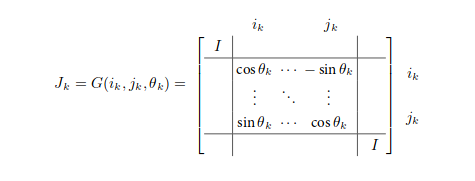
\includegraphics[width=0.8\textwidth]{figurest/figure_1.png} 
\end{minipage} 
\end{figure}
下面我们介绍一种适合并行计算的更新顺序:{\color{blue}红黑排序},即将二维网络点依次做红黑记号,如右图\\
在计算过程中,对未知量的值进行更新时,我们可以先更新红色节点,此时所使用的只是黑色节点的数据,然后再更新黑色节点,这时使用的是红色节点的数据.于是我们得到红黑排序G-S迭代方法.\\
\begin{figure}[h]%%图
	\centering  %插入的图片居中表示
	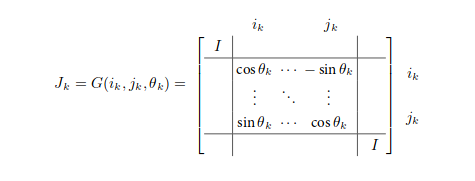
\includegraphics[width=0.7\linewidth]{figurest/figure_1.png}  %插入的图,包括JPG,PNG,PDF,EPS等,放在源文件目录下
	\caption{}  %图片的名称
	\label{fig:mcmthesis-logo}   %标签,用作引用
\end{figure}

\begin{tabular}{l}
\hline
{\color{blue}算法2.4}求解二维离散poisson方程的红黑排序G-S迭代方法\\
\hline
1:Choose an initial guess $v^{(0)}$\\
2: while not converge do\\
3:\qquad for $(i,j)$为红色节点 do\\
4:\qquad \qquad
$u_{i, j}^{(k+1)}=\frac{1}{4}\left(h^{2} f_{i, j}+u_{i+1, j}^{(k)}+u_{i-1, j}^{(k)}+u_{i, j+1}^{(k)}+u_{i, j-1}^{(k)}\right)$\\
5:\qquad end for\\
6:\qquad for $(i,j)$为黑色节点 do\\
7:\qquad \qquad
$u_{i, j}^{(k+1)}=\frac{1}{4}\left(h^{2} f_{i, j}+u_{i+1, j}^{(k+1)}+u_{i-1, j}^{(k+1)}+u_{i, j+1}^{(k+1)}+u_{i, j-1}^{(k+1)}\right)$\\
8:\qquad end for\\
9:end while\\
\hline
\end{tabular}\\
\subsubsection{SOR迭代}
在G-S算法的基础上,我们可以通过引入一个松弛参数$\omega$来加快收敛速度.这就是SOR (Successive Overrelaxation)算法,即将G-S算法中的第$k+1$步近似解与第k步近似解做一个加权平均:
\begin{align}
x^{(k+1)}=(1-\omega) x^{(k)}+\omega\left(D^{-1}\left(L x^{(k+1)}+U x^{(k)}\right)+D^{-1} b\right)\tag{6.10}
\end{align}
整理后即为
\begin{align}
x^{(k+1)}=(D-\omega L)^{-1}((1-\omega) D+\omega U) x^{(k)}+\omega(D-\omega L)^{-1} b\tag{6.11}
\end{align}
其中$\omega$称为{\color{blue}松弛参数}。\\
当$\omega=1$时,SOR即为G-S算法,当$\omega<$时,称为{\color{blue}低松弛(under relaxation)}算法,当$\omega>1$时,称为{\color{blue}超松弛(over relaxation)}算法.\\
SOR算法曾经在很长一段时间内是科学计算中求解线性方程组的首选方法。在大多数情况下,当$\omega>1$时会取得比较好的收敛效果.\\
SOR的迭代矩阵为
$$
G_{\mathrm{SOR}}=(D-\omega L)^{-1}((1-\omega) D+\omega U)
$$

对应的矩阵分裂为
$$
M=\frac{1}{\omega} D-L, \quad N=\frac{1-\omega}{\omega} D+U
$$
由({\color{blue}6.11})可得SOR迭代的分量形式为
$$
\begin{aligned} x_{i}^{(k+1)} &=(1-\omega) x_{i}^{(k)}+\frac{\omega}{a_{i i}}\left(b_{i}-\sum_{j=1}^{i-1} a_{i j} x_{j}^{(k+1)}-\sum_{j=i+1}^{n} a_{i j} x_{j}^{(k)}\right) \\ &=x_{i}^{(k)}+\frac{\omega}{a_{i i}}\left(b_{i}-\sum_{j=1}^{i-1} a_{i j} x_{j}^{(k+1)}-\sum_{j=i}^{n} a_{i j} x_{j}^{(k)}\right) \end{aligned}
$$
\begin{tabular}{l}
\hline
{\color{blue}算法2.5}求解线性方程组的SOR迭代方法\\
\hline
1:Choose an initial guess $x^{(0)}$\\
2: while not converge do\\
3:\qquad for $i=1$ to n do\\
4:\qquad \qquad
$x_{i}^{(k+1)}=(1-\omega) x_{i}^{(k)}+\frac{\omega}{a_{i i}}\left(b_{i}-\sum_{j=1}^{i-1} a_{i j} x_{j}^{(k+1)}-\sum_{j=i+1}^{n} a_{i j} x_{j}^{(k)}\right)$\\
5:\qquad end for\\
6:end while\\
\hline
\end{tabular}\\
SOR算法最大的优点是引入了松弛参数$\omega$,通过选取适当的$\omega$可以大大提高算法的收敛速度.\\
但是SOR算法最大的难点就是如何选取最优的参数\\
\begin{tabular}{l}
\hline
{\color{blue}算法2.4}求解二维离散poisson方程的红黑排序G-S迭代方法\\
\hline
1:Choose an initial guess $v^{(0)}$\\
2: while not converge do\\
3:\qquad for $(i,j)$为红色节点 do\\
4:\qquad \qquad
$u_{i, j}^{(k+1)}=(1-\omega) v_{i, j}^{(k)}+\omega\left(h^{2} f_{i, j}+u_{i+1, j}^{(k)}+u_{i-1, j}^{(k)}+u_{i, j+1}^{(k)}+\right.$
$u_{i, j-1}^{(k)} ) / 4$\\
5:\qquad end for\\
6:\qquad for $(i,j)$为黑色节点 do\\
7:\qquad \qquad
$u_{i, j}^{(k+1)}=(1-\omega) v_{i, j}^{(k)}+\omega\left(h^{2} f_{i, j}+u_{i+1, j}^{(k+1)}+u_{i-1, j}^{(k+1)}+u_{i, j+1}^{(k+1)}+\right.$
$u_{i, j-1}^{(k+1)} ) / 4$\\
8:\qquad end for\\
9:end while\\
\hline
\end{tabular}\\
\subsubsection{SSOR迭代方法}
将SOR算法中的L和U相交换,即可得迭代格式
$$
x^{(k+1)}=(D-\omega U)^{-1}((1-\omega) D+\omega L) x^{(k)}+\omega(D-\omega U)^{-1} b
$$
将这个迭代格式与SOR相结合,就可以得到下面的两步迭代方法
$$
\left\{\begin{array}{l}{x^{\left(k+\frac{1}{2}\right)}=(D-\omega L)^{-1}[(1-\omega) D+\omega U] x^{(k)}+\omega(D-\omega L)^{-1} b} \\ {x^{(k+1)}=(D-\omega U)^{-1}[(1-\omega) D+\omega L] x^{\left(k+\frac{1}{2}\right)}+\omega(D-\omega U)^{-1} b}\end{array}\right.
$$
这就是{\color{blue}SSOR迭代}(对称超松弛)算法,相当于将L与U同等看待,交替做两次SOR迭代.\\
消去中间迭代量$x^{(k+\frac{1}{2})}$,可得
$$
x^{(k+1)}=G_{\mathrm{SSOR}} x^{(k)}+g
$$
其中迭代矩阵
$$
G_{\mathrm{SSOR}}=(D-\omega U)^{-1}[(1-\omega) D+\omega L](D-\omega L)^{-1}[(1-\omega) D+\omega U]
$$
对应的矩阵分裂为
$$
\begin{aligned} M &=\frac{1}{\omega(2-\omega)}\left[D-\omega(L+U)+\omega^{2} L D^{-1} U\right] \\ &=\frac{1}{\omega(2-\omega)}(D-\omega L) D^{-1}(D-\omega U) \\ N &=\frac{1}{\omega(2-\omega)}[(1-\omega) D+\omega L] D^{-1}[(1-\omega) D+\omega U] \end{aligned}
$$
对于某些特殊问题, SOR算法不收敛,但仍然可能构造出收敛的SSOR算法.\\
一般来说, SOR算法的渐进收敛速度对参数$\omega$比较敏感,但SSOR对参数$\omega$不太敏感.\\
({\color{blue} Poisson SOR omega.m,Poisson SSOR omega.m)})\\
\subsubsection{AOR迭代}
Hadjidimos于1978年提出了AOR (Accelerated over-relaxation,快速松弛)算法,迭代矩阵为
$$
G_{\mathrm{AOR}}=(D-\gamma L)^{-1}[(1-\omega) D+(\omega-\gamma) L+\omega U]
$$
其中$\gamma$和$\omega$为松弛参数.对应的矩阵分解为
$$
M=\frac{1}{\omega}(D-\gamma L), \quad N=\frac{1}{\omega}[(1-\omega) D+(\omega-\gamma) L+\omega U]
$$
\begin{tabular}{l}
\qquad  (1)当$\gamma=\omega$时, AOR算法即为SOR算法;\\
\qquad  (2)当$\gamma=\omega=1$时, AOR算法即为G-S算法;\\
\qquad  (3)当$\gamma=0,\omega=1$时, AOR算法即为Jacobi算法
\end{tabular}
与SSOR类似,我们也可以定义SAOR算法.
\subsubsection{Richardson算法}
Richardson算法是一类形式非常简单的算法,其迭代格式为
$$
x^{(k+1)}=x^{(k)}+\omega\left(b-A x^{(k)}\right), \quad k=0,1,2, \ldots
$$
对应的矩阵分裂和迭代矩阵分别为
$$
M=\frac{1}{\omega} I, \quad N=\frac{1}{\omega} I-A, \quad G_{\mathrm{R}}=I-\omega A
$$
如果在每次迭代时取不同的参数,即
$$
x^{(k+1)}=x^{(k)}+\omega_{k}\left(b-A x^{(k)}\right), \quad k=0,1,2, \ldots
$$
则称为nonstationary Richardson算法.
{\color{blue}定理}设$A \in \mathbb{R}^{n \times n}$是对称正定矩阵,$\lambda_1$和$\lambda_n$分别是$A$的最大和最小特征值,则Richardson算法收敛当且仅当
$$
0<\omega<\frac{1}{\lambda_{1}}
$$
最优参数为
$$
\omega_{*}=\arg \min _{\omega} \rho\left(G_{\mathrm{R}}\right)=\frac{2}{\lambda_{1}+\lambda_{n}}
$$
即当$\omega=\omega_{*}$时,迭代矩阵的谱半径达到最小,且有
$$
\rho\left(G_{\mathrm{R}}\right)=\left\{\begin{array}{ll}{1-\omega \lambda_{n}} & {\text { if } \omega \leq \omega} \\ {\frac{\lambda_{1}-\lambda_{n}}{\lambda_{1}+\lambda_{n}}=\frac{\kappa(A)-1}{\kappa(A)+1}} & {\text { if } \omega=\omega} \\ {\omega \lambda_{1}-1} & {\text { if } \omega \geq \omega}\end{array}\right.
$$
\subsubsection{分块迭代方法}
前面介绍的迭代方法可以推广到分块情形.将$A$写成如下的分块形式
$$
A=\left[\begin{array}{cccc}{A_{11}} & {A_{12}} & {\cdots} & {A_{1 p}} \\ {A_{21}} & {A_{22}} & {\cdots} & {A_{2 p}} \\ {\vdots} & {\vdots} & {\ddots} & {\vdots} \\ {A_{p 1}} & {A_{p 2}} & {\cdots} & {A_{P P}}\end{array}\right]
$$
设$A=D-L-U$,其中$D,-L,-U$分别是A的快对角,块严格下三角矩阵和块严格上三角矩阵。则相应的分块Jacobi,分块Gauss-Seidel和分块SOR算法分别为
\begin{figure}[h]
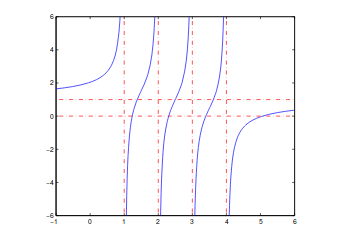
\includegraphics[width=0.8\textwidth]{figurest/figure_2.png} 
\end{figure}
\begin{itemize}
\item {\color{blue}分块Jacobi迭代}$$
A_{i i} \boldsymbol{x}_{i}^{(k+1)}=\boldsymbol{b}_{i}-\sum_{j=1, j \neq i}^{p} A_{i j} \boldsymbol{x}_{j}^{(k)}, \quad i=1,2, \ldots, p
$$
\item {\color{blue}分块Gauss-seidel迭代}$$
A_{i i} \boldsymbol{x}_{i}^{(k+1)}=\boldsymbol{b}_{i}-\sum_{j=1}^{i-1} A_{i j} \boldsymbol{x}_{j}^{(k+1)}-\sum_{j=i+1}^{p} A_{i j} \boldsymbol{x}_{j}^{(k)}, \quad i=1,2, \ldots, p
$$
\item {\color{blue}分块SOR迭代}$$
\begin{array}{c}{\boldsymbol{x}_{i}^{(k+1)}=(1-\omega) \boldsymbol{x}_{i}^{(k)}+\omega A_{i i}^{-1}\left(\boldsymbol{b}_{i}-\sum_{j=1}^{i-1} A_{i j} \boldsymbol{x}_{j}^{(k+1)}-\sum_{j=i+1}^{p} A_{i j} \boldsymbol{x}_{j}^{(k)}\right)} \\ {i=1,2, \ldots, p}\end{array}
$$
\end{itemize}
%\newpage
\subsection{收敛性分析}
%\newpage
\subsubsection{定常迭代方法的收敛性}
{\color{blue}定义(迭代方法的收敛性)}如果对于任意的初始向量$x^{(0)}$,都有
$$\lim_{k\to \infty}x^{(k)}\to x_*$$
则称迭代格式{\color{blue}6.7}是{\color{blue}收敛}的,否则就称其为{\color{blue}发散}的。\\
基于矩阵分裂的迭代方法,其收敛性取决于迭代矩阵的谱半径.
\subsection*{矩阵谱半径}
设$A \in \mathbb{R}^{n \times n}$,则称
$$
\rho(A) \triangleq \max _{\lambda \in \sigma(A)}|\lambda|
$$
为$A$的{\color{blue}谱半径},其中$\sigma(A)$表示$A$的所有特征值组成的集合。\\
谱半径与矩阵范数之间有如下的关系.\\
{\color{blue}引理(谱半径与范数的关系)}设$G \in \mathbb{R}^{n \times n}$,则
\begin{itemize}
\item (1)对任意算子范数,有$\rho(G) \leq\|G\|$;
\item (2)反之,对任意$\varepsilon>0$,都存在一个算子范数$\|\cdot\|_{\varepsilon}$,使得$| G \|_{\varepsilon} \leq\rho(G)+\varepsilon$,其中范数$\|\cdot\|_{\varepsilon}$依赖于$G$和$\varepsilon$.所以,若$\rho(G)<1$,则存在算子范数$\|\cdot\| \varepsilon$,使得$| G \|_{\varepsilon}<1$;
\end{itemize}
由此,我们可以立即得到下面的结论.\\
{\color{blue}定理}设矩阵$G \in \mathbb{R}^{n \times n}$,则$\lim _{k \rightarrow \infty} G^{k}=0$当且仅当$\rho(G)<1$.
下面的结论是谱半径与算子范数之间的一个非常重要的性质。\\
{\color{blue}引理}设$G \in \mathbb{R}^{n \times n}$,则对任意算子范数$\|\cdot\|$,有
$$
\rho(G)=\lim _{k \rightarrow \infty}\left\|G^{k}\right\|^{\frac{1}{k}}
$$
\subsection*{迭代方法收敛性判断}
首先给出一个迭代方法收敛的充分条件\\
{\color{blue}引理}若存在算子范数$\|\cdot\|$,使得$| G \|<1$,则迭代方法6.7收敛.\\
我们记$e^{(k)} \triangleq x^{(k)}-x$为第$k$步迭代解$x^{(k)}$的{\color{blue}误差向量}.\\
{\color{blue}定理(收敛性定理)}对任意迭代初始向量$x^{(0)}$,迭代方法6.7收敛的充要条件是$\rho(G)<1$.\\
{\color{blue}定义}设$G$是迭代矩阵,则迭代方法6.7的{\color{blue}平均收敛速度}定义为
$$
R_{k}(G) \triangleq-\ln \left\|G^{k}\right\|^{\frac{1}{k}}
$$,
{\color{blue}渐进收敛速度}定义为
$$
R(G) \triangleq \lim _{k \rightarrow \infty} R_{k}(G)=-\ln \rho(G)
$$
平均收敛速度与迭代步数和所用的范数有关,但渐进收敛速度只依赖于迭代矩阵的谱半径.\\
{\color{blue}定理}考虑算法6.7.如果存在某个算子范数$\|\cdot\|$使得$\|G\|=q<1$,则
\begin{itemize}
\item (1)$\left\|x^{(k)}-x_{*}\right\| \leq q^{k}\left\|x^{(0)}-x_{*}\right\|$
\item (2)$\left\|x^{(k)}-x_{+}\right\| \leq \frac{q}{1-q}\left\|x^{(k)}-x^{(k-1)}\right\|$
\item (3)$\left\|x^{(k)}-x_{*}\right\| \leq \frac{q^{k}}{1-q}\left\|x^{(1)}-x^{(0)}\right\|$
\end{itemize}
一般来说,好的迭代方法应该满
\begin{itemize}
\item(1)$\rho(G)$很小;
\item(2)以$M$为系数矩阵的线性方程组比较容易求解
\end{itemize}
\subsubsection{二维离散Poisson方程情形}
{\color{blue}充要条件}:迭代矩阵的谱半径小于1.\\
{\color{blue}充分条件}:迭代矩阵的某个算子范数小于1.\\
对于二维离散Poisson方程,系数矩阵为
$$
A=T=I \otimes T_{n}+T_{n} \otimes I
$$
故Jacobi算法的迭代矩阵为

\begin{align*}
G_{\mathrm{J}}=D^{-1}(L+U)=(4 I)^{-1}(4 I-T)=I-\frac{1}{4} T
\tag {6.12}
\end{align*}

由于$T$的特征值为
$$
\lambda_{i}+\lambda_{j}=2\left(1-\cos \frac{\pi i}{n+1}\right)+2\left(1-\cos \frac{\pi j}{n+1}\right)
$$
所以$G_{\mathrm{J}}$的特征值为
$$
1-\frac{1}{4}\left(\lambda_{i}+\lambda_{j}\right)=\frac{1}{2}\left(\cos \frac{\pi i}{n+1}+\cos \frac{\pi j}{n+1}\right)
$$
故
$$
\rho\left(G_{\mathrm{J}}\right)=\frac{1}{2} \max _{i, j}\left\{\left|\cos \frac{\pi i}{n+1}+\cos \frac{\pi j}{n+1}\right|\right\}=\cos \frac{\pi}{n+1}<1
$$
即Jacobi算法是收敛的.
注意当$n$越来越大时,$\kappa(T) \rightarrow \infty$,即$T$越来越病态,此时$\rho\left(G_{1}\right) \rightarrow 1$,即Jacobi算法收敛越来越慢.\\
{\color{blue}问题越病态可能就越难求解}\\
\subsection*{\color{blue}G-S算法和SOR算法}
{\color{blue}性质}设$G_{\mathrm{GS}}$和$G_{\mathrm{SOR}}$分别表示求解二维Poisson方程的红黑排序的G-S算法和SOR算法的迭代矩阵,则有
\begin{align*}
\rho\left(G_{\mathrm{GS}}\right)=\rho\left(G_{\mathrm{J}}\right)^{2}=\cos ^{2} \frac{\pi}{n+1}<1
\tag{6.13}
\end{align*}
\begin{align*}
\rho\left(G_{\mathrm{SOR}}\right)=\frac{\cos ^{2} \frac{\pi}{n+1}}{\left(1+\sin \frac{\pi}{n+1}\right)^{2}}<1, \quad \omega=\frac{2}{1+\sin \frac{\pi}{n+1}}
\tag{6.14}
\end{align*}
在上述结论中, SOR算法中的$\omega$是最优参数,即此时的$\rho\left(G_{\mathrm{SOR}}\right)$最小.
\subsection*{SOR与Jacobi}
由Taylor公式可知,当$n$很大时,有
$$
\begin{aligned} \rho\left(G_{\mathrm{J}}\right) &=\cos \frac{\pi}{n+1} \approx 1-\frac{\pi^{2}}{2(n+1)^{2}}=1-O\left(\frac{1}{n^{2}}\right) \\ \rho\left(G_{\mathrm{SOR}}\right) &=\frac{\cos ^{2} \frac{\pi}{n+1}}{\left(1+\sin \frac{\pi}{n+1}\right)^{2}} \approx 1-\frac{2 \pi}{n+1}=1-O\left(\frac{1}{n}\right) \end{aligned}
$$
由于当$n$很大时有
$$
\left(1-\frac{1}{n}\right)^{k} \approx 1-\frac{k}{n}=1-\frac{k n}{n^{2}} \approx\left(1-\frac{1}{n^{2}}\right)^{k n}
$$
即SOR迭代$k$步后误差的减小量与Jacobi迭代$kn$步后误差减小量差不多.因此,取最优参数的$SOR$算法的收敛速度大约是$Jacobi$算法的$n$倍.\\
事实上,当$n$很大时,这三个算法的收敛速度都很慢.\\
{\color{blue}例}\quad 已知二维Poisson方程
$$
\left\{\begin{array}{ll}
{-\Delta u(x, y)=-1,} & {(x, y) \in \Omega} \\ 
{u(x, y)=\frac{x^{2}+y^{2}}{4},} & {(x, y) \in \partial \Omega}\end{array}\right.
$$
其中$\Omega=(0,1) \times(0,1)$.该方程的解析解是$u(x, y)=\frac{x^{2}+y^{2}}{4}$.用五点差分格式离散后得到一个线性方程组,分别用Jacobi, G-S和SOR算法计算这个方程组的解,并比较收敛效果
\begin{figure}[h]
\centering 
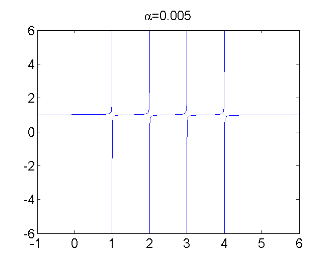
\includegraphics[width=0.8\textwidth]{figurest/figure_3.png} 
\end{figure}
\subsubsection{不可约对角占优}
这里我们考虑A是严格对角占优或不可约弱对角占优情形.
{\color{blue}定理}\quad 设$A \in \mathbb{R}^{n \times n}$,若A严格对角占优,则Jacobi算法和G-S算法都收敛,且
$$
\left\|G_{\mathrm{GS}}\right\|_{\infty} \leq\left\|G_{\mathrm{J}}\right\|_{\infty}<1
$$
{\color{blue}定理}\quad 设$A \in \mathbb{R}^{n \times n}$若A是弱对角占优且不可约,则Jacobi算法和G-S算法都收敛,且$\rho\left(G_{\mathrm{GS}}\right)<\rho\left(G_{\mathrm{J}}\right)<1$
二维离散Poisson方程是弱行对角占优且不可约,故对Jacobi算法和G-S算法都收敛.\\
上述定理中的结论对一般矩阵并不成立:{\color{blue}对某些矩阵, Jacobi算法收敛,但G-S算法却不一定收敛}.\\
关于SOR方法,我们有下面的结论\\
设$A \in \mathbb{R}^{n \times n}$,若A严格对角占优且$0<\omega \leq 1$,则SOR方法收敛.\\
{\color{blue}定理}\quad 设$A \in \mathbb{R}^{n \times n}$若A是弱对角占优且不可约,且$0<\omega \leq 1$则SOR方法收敛.
\subsubsection{对称正定矩阵}
在给出收敛性结论之前,也介绍两个需要用到的引理.\\
{\color{blue}引理}\quad 设$A \in \mathbb{C}^{n \times n}$,Hermite对称,且$A=M-N$是$A$的一个矩阵分裂,则$M^{*}+N$也是Hermite对称,且对任意$x \in \mathbb{C}^{n}$有
$$
x^{*} A x-\tilde{x}^{*} A \tilde{x}=u^{*}\left(M^{*}+N\right) u
$$
其中$\tilde{x}=M^{-1} N x, u=x-\tilde{x}$
{\color{blue}定理}\quad 设$A \in \mathbb{R}^{n \times n}$对称,且$A=M-N$是$A$的一个矩阵分裂.
\begin{itemize}
\item (1)如果$A$和$M^{T}+N$都是正定矩阵,则$M$非奇异且$\rho\left(M^{-1} N\right)<1$
\item (2)如果$\rho\left(M^{-1} N\right)<1$且$M^{T}+N$正定,则$A$正定.
\end{itemize}
我们首先给出SOR迭代收敛的一个必要条件.
{\color{blue}定理}对于SOR算法,有$\rho\left(G_{\mathrm{SOR}}\right) \geq|1-\omega|$,故SOR算法收敛的必要条件是$0<\omega<2$.
{\color{blue}定理}\quad 设$A \in \mathbb{R}^{n \times n}$对称正定.
\begin{itemize}
\item (1)若$2D$正定且Jacobi迭代收敛,则$A$正定
\item (2)若$D$正定,且存在$\omega \in(0,2)$使得SOR (或SSOR)收敛,则$A$正定
\item (3)若$D$正定,且G-S迭代收敛,则$A$正定.
\end{itemize}
\subsubsection{相容次序矩阵}
针对一类特殊的矩阵,这三种迭代方法的谱半径之间存在一种特殊关系.\\
{\color{blue}定义}设$A \in \mathbb{R}^{n \times n}$,如果存在一个置换矩阵$P$,使得
\begin{align}
P A P^{T}=\left[\begin{array}{cc}{D_{1}} & {F} \\ {E} & {D_{2}}\end{array}\right]\tag{6.15}
\end{align}
其中$D_{1}, D_{2}$为对角矩阵,则称$A$具有{\color{blue}性质A}.
{\color{blue}例}\quad 对于二维离散Poisson方程,系数矩阵$T_{N^{2}}$具有性质$A$.事实上,设$\tilde{T}_{N^{2}}$为模型问题采用红黑排序后的系数矩阵,则$\tilde{T}_{N^{2}}$具有({\color{blue}6.15})的结构.\\
我们首先给出一个性质.\\
{\color{blue}引理}\quad 设$B \in \mathbb{R}^{n \times n}$具有下面的结构
$$
B=\left[\begin{array}{cc}{0} & {B_{12}} \\ {B_{21}} & {0}\end{array}\right]
$$
令$B_L$和$B_U$分别表示$B$的下三角和上三角部分,则
\begin{itemize}
\item (1)若$\mu$是$B$的特征值,则$-\mu$也是$B$的特征值;
\item (2)$B(\alpha)$的特征值与无关,其中
$$
B(\alpha)=\alpha B_L+\frac{1}{\alpha}B_U,\qquad \alpha \ne 0
$$
\end{itemize}
$B(\alpha)+\beta I$的特征值也与$\alpha$无关,其中$\beta$为任意常数.\\
该结论可以推广到块三对角形式,见习题.
设$A \in \mathbb{R}^{n \times n}$的对角线元素全不为零,记$\tilde{L}=D^{-1} L, \tilde{U}=D^{-1} U$.\\
{\color{blue}定义}设$A \in \mathbb{R}^{n \times n}$的对角线元素全不为零,$A=D(I-\tilde{L}-\tilde{U})$若矩阵$G(\alpha)=\alpha \tilde{L}+\frac{1}{\alpha} \tilde{U}$的特征值与$\alpha$无关,则称$A$具有相容次序.\\
设$A$的对角线元素全不为零,若$A$具有性质$A$,则存在置换矩阵$P$,使得$P A P^{T}$具有相容次序.\\
{\color{blue}定理}\quad 设$A$有相容次序且$\omega \neq 0$,则下列命题成立
\begin{itemize}
\item (1)Jacobi迭代矩阵$G_{\mathrm{l}}$的特征值正负成对出现;
\item (2)若$\mu$是$G_{\mathrm{J}}$的特征值且$\lambda$满足
\begin{align}
	(\lambda+\omega-1)^{2}=\lambda \omega^{2} \mu^{2}\tag{6.16}
\end{align}
则$\lambda$是$SOR$迭代矩阵$G_{\mathrm{SOR}}$的一个特征值;
\item (3)反之,若$\lambda \neq 0$是$G_{\mathrm{SOR}}$的一个特征值且$\mu$满足(6.16),则$\mu$是$G_{\mathrm{J}}$的一个特征值.
\end{itemize}
{\color{blue}推论}\quad 若$A$具有相容次序,则$\rho\left(G_{\mathrm{GS}}\right)=\rho\left(G_{\mathrm{J}}\right)^{2}$,即当Jacobi算法收敛时,G-S算法比Jacobi算法快一倍
{\color{blue}例}\qquad 采用红黑排序的二维离散Poisson方程,系数矩阵$\tilde{T}_{N^{2}}$具有相容次序,故有$\rho\left(G_{\mathrm{GS}}\right)=\rho\left(G_{\mathrm{J}}\right)^{2}$.\\
下面是关于SOR算法的最优参数选取.\\
{\color{blue}定理}\qquad 设$A$具有相容次序,$G_{\mathrm{l}}$的特征值全部为实数,且$\rho_{J}=\rho\left(G_{\mathrm{J}}\right)<1$,则SOR算法的最优参数为
$$
\omega_{o p t}=\frac{2}{1+\sqrt{1-\rho_{J}^{2}}}
$$
此时
$$
\rho\left(G_{\mathrm{SOR}}\right)=\omega_{o p t}-1=\frac{\rho_{J}^{2}}{\left(1+\sqrt{1-\rho_{J}^{2}}\right)^{2}}
$$
进一步,有
$$
\rho\left(G_{\mathrm{SOR}}\right)=\left\{\begin{array}{ll}{\omega-1,} & {\omega_{o p t} \leq \omega \leq 2} \\ {1-\omega+\frac{1}{2} \omega^{2} \rho_{J}^{2}+\omega \rho_{J} \sqrt{1-\omega+\frac{1}{4} \omega^{2} \rho_{J}^{2}},} & {0<\omega \leq \omega_{o p t}}\end{array}\right.
$$
{\color{blue}例}\qquad 采用红黑排序的二维离散Poisson问题的系数矩阵$\tilde{T}_{N^{2}}$具有相容次序,且$G_{\mathrm{l}}$是对称的,即$G_{\mathrm{l}}$的特征值都是实的.又由系数矩阵的弱对角占优和不可约性质可知$\rho\left(G_{1}\right)<1$,故上述定理的条件均满足.
\subsection{加速算法}
当迭代解$x^{(0)}, x^{(1)}, x^{(2)}, \ldots, x^{(k)}$已经计算出来后,我们可以对其进行组合,得到一个新的近似解,这样就可以对原算法进行加速
\subsubsection{外推技术}
设原迭代格式为
\begin{align*}
x^{(k+1)}=G x^{(k)}+b
\tag{6.17}
\end{align*}
由$x^{(k)}$和$x^{(k+1)}$加权组合后可得新的近似解
\begin{align*}
x^{(k+1)}=(1-\omega) x^{(k)}+\omega\left(G x^{(k)}+b\right)
\tag{6.18}
\end{align*}
其中$\omega$是参数.这种加速方法就称为{\color{blue}外推算法}.\\
为了使得迭代格式(6.18)尽可能快地收敛,需要选择$\omega$使得其迭代矩阵$G_{\omega} \triangleq(1-\omega) I+\omega G$的谱半径尽可能地小.假设$G$的特征值都是实数,且最大特征值和最小特征值分别为$\lambda_{1}$和$\lambda_{n}$.于是
$$
\rho\left(G_{\omega}\right)=\max _{\lambda \in \sigma(G)}|(1-\omega)+\omega \lambda|=\max \left\{\left|1-\omega+\omega \lambda_{1}\right|,\left|1-\omega+\omega \lambda_{n}\right|\right\}
$$
{\color{blue}定理}\qquad 设$G$的特征值都是实数,其最大和最小特征值分别为$\lambda_{1}$和$\lambda_{n}$,且1$\notin\left[\lambda_{n}, \lambda_{1}\right]$,则
$$
\omega_{*}=\arg \min _{\omega} \rho\left(G_{\omega}\right)=\frac{2}{2-\left(\lambda_{1}+\lambda_{n}\right)}
$$
此时
$$
\rho\left(G_{\omega_{*}}\right)=1-\left|\omega_{*}\right| d
$$
其中$d$是$1$到$\left[\lambda_{n}, \lambda_{1}\right]$的距离,即当$\lambda_{n} \leq \lambda_{1}<1$时,$d=\lambda_{n}-1$.\\
由定理可知,$\rho\left(G_{\omega_{*}}\right)=1-\left|\omega_{*}\right| d$且当$\omega_{*} \neq 1$时,外推迭代(6.18)比原迭代方法收敛要更快一些.\\
最优参数依赖于原迭代矩阵$G$的特征值,因此实用性不强.在实际应用时可以估计特征值所在的区间$[a, b]$,然后用$a,b$代替$\lambda_{n}$和$\lambda_{1}$.
\subsection*{JOR算法}
对$Jacobi$迭代进行外推加速,则可得$JOR (Jacobi over-relaxation)$算法:
$$
\begin{aligned} x^{(k+1)} &=(1-\omega) x^{(k)}+\omega\left(D^{-1}(L+U) x^{(k)}+D^{-1} b\right) \\ &=x^{(k)}+\omega D^{-1}\left(b-A x^{(k)}\right), \quad k=0,1,2, \ldots \end{aligned}
$$
{\color{blue}定理}\qquad 设$A$对称正定.若
$$
0<\omega<\frac{2}{\rho\left(D^{-1} A\right)}
$$
则JOR算法收敛.\\
\subsection{Chebyshev加速}
本节对外推技巧进行推广.\\
假定通过迭代格式(6.17)已经计算出$x^{(0)}, x^{(1)}, \ldots, x^{(k)}$,下面考虑如何将这些近似解进行组合,以便得到更精确的近似解.\\
记$\varepsilon_{k}=x^{(k)}-x_{*}$为第$k$步迭代解的误差,则有
$$
\varepsilon_{k}=G \varepsilon_{k-1}=G^{2} \varepsilon_{k-2}=\cdots=G^{k} \varepsilon_{0}
$$
设$\tilde{x}^{(k)}$为$x^{(0)}, x^{(1)}, \ldots, x^{(k)}$的一个线性组合,即
\begin{align*}
\tilde{x}^{(k)}=\alpha_{0} x^{(0)}+\alpha_{1} x^{(1)}+\cdots+\alpha_{k} x^{(k)}
\tag{6.19}
\end{align*}
其中$\alpha_{i}$为待定系数,且满足$\sum_{i=0}^{k} \alpha_{i}=1$.于是
\begin{align*}
\tilde{x}^{(k)}-x_{*}=\alpha_{0} \varepsilon_{0}+\alpha_{1} G \varepsilon_{0}+\cdots+\alpha_{k} G^{k} \varepsilon_{0} \triangleq p_{k}(G) \varepsilon_{0}
\tag{6.20}
\end{align*}
其中$p_{k}(t)=\sum_{i=0}^{k} \alpha_{i} t^{i}$为$k$次多项式,且满足$p_{k}(1)=1$.\\
我们希望通过适当选取参数$\alpha_i$,使得$\tilde{x}^{(k)}-x_*$尽可能地小,即使得$\tilde{x}^{(k)}$收敛到$x_*$速度远远快于$x^{(k)}$收敛到$x$速度.这种加速方法就称为{\color{blue}多项式加速}或{\color{blue}半迭代方法(semi-iterative method)}\\
{\color{blue}例}\qquad 设$p_{n}(t)$为$G$的特征多项式,则$p_{n}(G)=0$,所以选取$\alpha_i$为$p_n$的系数,则$\tilde{x}^{(n)}-x_{*}=0$.但这种选取方法不实用,原因是:
\begin{itemize}
\item (1)$p_{n}(t)$的系数并不知道;
\item (2)我们通常希望收敛所需的迭代步数$\ll n$.
\end{itemize}
下面讨论参数$\alpha_i$的较实用的选取方法.由(6.20)可知
$$\left\|\tilde{x}^{(k)}-x_{*}\right\|_{2}=\left\|p_{k}(G) \varepsilon_{0}\right\|_{2} \leq\left\|p_{k}(G)\right\|_{2} \cdot\left\|\varepsilon_{0}\right\|_{2}$$
因此我们需要求解下面的极小化问题
\begin{align*}
\min _{p \in \mathbb{P}_{k}, p(1)=1}\|p(G)\|_{2}
\tag{6.21}
\end{align*}
其中$\mathbb{P}_{k}$表示所有次数不超过k的多项式组成的集合.\\
一般来说,这个问题是非常困难的.\\
但在一些特殊情况下,我们可以给出其最优解.\\
假设迭代矩阵$G$是对称的,即$G$存在特征值分解$Schur$标准型为
$$
G=U \Lambda U^{*}
$$
其中$\Lambda$是实对角矩阵,$U$是酉矩阵.于是有
\begin{align*}
\begin{array}{ll}
	\min _{p \in \mathbb{P}_{k, P}(1)=1}\|p(G)\|_{2}&{=\min _{p \in \mathbb{P}_{k, p}(1)=1}^{\min }\|p(\Lambda)\|_{2}} \\ {}&{=\min _{p \in \mathbb{P}_{k, p}(1)=1} \max _{1 \leq i \leq n}\left\{\left|p\left(\lambda_{i}\right)\right|\right\}} \\ {}&{ \leq \min _{p \in \mathbb{P}_{k, p}(1)=1} \max _{\lambda \in\left[\lambda_{n}, \lambda_{1}\right]}\{|p(\lambda)|\}}\end{array}
\tag{6.22}
\end{align*}
其中$\lambda_{1}, \lambda_{n}$分别表示$G$的最大和最小特征值.\\
这是带归一化条件的多项式最佳一致逼近问题(与零的偏差最小).\\
该问题的解与著名的{\color{blue}Chebyshev多项式}有关.\\
\subsection*{Chebyshev多项式}
Chebyshev多项式$T_{k}(t)$可以通过下面的递归方式来定义:
\begin{align*}
\begin{array}{l}{T_{0}(t)=1, \quad T_{1}(t)=t} \\ {T_{k}(t)=2 t T_{k-1}(t)-T_{k-2}(t), k=2,3, \ldots}\end{array}
\tag{6.23}
\end{align*}
也可以直接由下面的式子定义
$$
T_{k}(t)=\frac{1}{2}\left[\left(t+\sqrt{t^{2}-1}\right)^{k}+\left(t+\sqrt{t^{2}-1}\right)^{-k}\right]
$$
或者
$$
T_{k}(t)=\left\{\begin{array}{ll}{\cos (k \text { arccost }),} & {|t| \leq 1} \\ {\cosh (k \operatorname{arccosh} t),} & {|t|>1}\end{array}\right.
$$
Chebyshev的一个重要性质是下面的最小最大性质.\\
{\color{blue}定理}设$\eta \in \mathbb{R}$满足$|\eta|>1$,则下面的最小最大问题
$$
\min _{p(t) \in \mathbb{P}_{k}, p(\eta)=1-1 \leq t \leq 1}|p(t)|
$$
的唯一解为
$$
\tilde{T}_{k}(t) \triangleq \frac{T_{k}(t)}{T_{k}(\eta)}
$$
通过简单的仿射变换,该定理的结论可以推广到一般区间.
{\color{blue}定理}\qquad 设$\alpha, \beta, \eta \in \mathbb{R}$满足$\alpha<\beta$且$|\eta| \notin[\alpha, \beta]$.则下面的最小最大问题
$$
\min _{p(t) \in \mathbb{P}_{k, p}(\eta)=1} \max _{\alpha \leq x \leq \beta}|p(t)|
$$
的唯一解为
$$
\hat{T}_{k}(t) \triangleq \frac{T_{k}\left(\frac{2 t-(\beta+\alpha)}{\beta-\alpha}\right)}{T_{k}\left(\frac{2 \eta-(\beta+\alpha)}{\beta-\alpha}\right)}
$$
\subsection*{Chebyshev加速方法}
\begin{enumerate}[(1)]
\item 迭代矩阵$G$的特征值都是实数;
\item 迭代矩阵谱半径$\rho=\rho(G)<1$,故$\lambda(G) \in[-\rho, \rho] \subset(-1,1)$
\end{enumerate}
于是最小最大问题(6.22)就转化为
$$
\min _{p \in \mathbb{P}_{k}, p(1)=1} \max _{\lambda \in[-\rho, \rho]}\{|p(\lambda)|\}
$$
由于$1 \neq[-\rho, \rho]$根据定理4.4,上述问题的解为
$$
p_{k}(t)=\frac{T_{k}(t / \rho)}{T_{k}(1 / \rho)}
$$
\subsection*{$\tilde{x}^{(k)}$的计算}
我们无需先计算$x^{(0)}, x^{(1)}, \ldots, x^{(k)}$,然后通过线性组合(6.19)来计算$\tilde{x}^{(k)}$事实上,我们可以通过Chebyshev多项式的三项递推公式(6.23),由$\tilde{x}^{(k-1)}$和$\tilde{x}^{(k-2)}$直接计算出$\tilde{x}^{(k)}$.这样做的另一个好处是无需存储所有的$\tilde{x}^{(i)}$.具体的推导公式如下:\\
令$\mu_{k}=\frac{1}{T_{k}(1 / \rho)}$,即$T_{k}(1 / \rho)=\frac{1}{\mu_{k}}$.由三项递推公式(6.23)可得
$$
\frac{1}{\mu_{k}}=\frac{2}{\rho} \cdot \frac{1}{\mu_{k-1}}-\frac{1}{\mu_{k-2}}
$$
所以
$$
\begin{aligned} \tilde{x}^{(k)}-x_{*}=p_{k}(G) \varepsilon_{0} &=\mu_{k} T_{k}(G / \rho) \varepsilon_{0} \\ &=\mu_{k}\left[\frac{2 G}{\rho} \cdot \frac{1}{\mu_{k-1}}\left(\tilde{x}^{(k-1)}-x_{*}\right)-\frac{1}{\mu_{k-2}}\left(\tilde{x}^{(k-2)}-x_{*}\right)\right] \end{aligned}
$$
整理后可得
$$
\boxed{\tilde{x}^{(k)}=\frac{2 \mu_{k}}{\mu_{k-1}} \cdot \frac{G}{\rho} \tilde{x}^{(k-1)}-\frac{\mu_{k}}{\mu_{k-2}} \tilde{x}^{(k-2)}+d_{k}}
$$
其中
$$
\begin{aligned} d_{k} &=x_{*}-\frac{2 \mu_{k}}{\mu_{k-1}} \cdot \frac{G}{\rho} x_{*}+\frac{\mu_{k}}{\mu_{k-2}} x_{*} \\ &=x^{*}-\frac{2 \mu_{k}}{\mu_{k-1}} \cdot \frac{x_{*}-g}{\rho}+\frac{\mu_{k}}{\mu_{k-2}} x_{*} \\ &=\mu_{k}\left(\frac{1}{\mu_{k}}-\frac{2}{\rho \mu_{k-1}}+\frac{1}{\mu_{k-2}}\right) x_{*}+\frac{2 \mu_{k} g}{\mu_{k-1} \rho} \\ &=\frac{2 \mu_{k} g}{\mu_{k-1} \rho} \end{aligned}
$$
由此,我们可以得到迭代格式(6.17)的Chebyshev加速算法.\\
\begin{tabular}{l}
\hline
{\color{blue}算法4.1}Chebyshev加速算法\\
\hline
1:Set $\mu_{0}=1, \mu_{1}=\rho=\rho(G), \tilde{x}^{(0)}=x^{(0)}, k=1$\\
2:compute$\tilde{x}^{(1)}=G x^{(0)}+g$\\
3:while not converge do\\
4:\qquad$k=k+1$\\
5:\qquad$\mu_{k}=\left(\frac{2}{\rho} \cdot \frac{1}{\mu_{k-1}}-\frac{1}{\mu_{k-2}}\right)^{-1}$\\
6:\qquad$\tilde{x}^{(k)}=\frac{2 \mu_{k}}{\mu_{k-1}} \cdot \frac{G}{\rho} \tilde{x}^{(k-1)}-\frac{\mu_{k}}{\mu_{k-2}} \tilde{x}^{(k-2)}+\frac{2 \mu_{k}}{\mu_{k-1} \rho} \cdot g$\\
7:end while\\
\hline
\end{tabular}
该算法的每步迭代的整体运算量与原迭代格式基本相当.\\
设$\lambda(G) \in[\alpha, \beta]$,且$-1<\alpha \leq \beta<1$,则我们也可以构造出相应的Chebyshev加速算法.\\
\subsection*{SSOR算法的Chebyshev加速}
SSOR迭代矩阵为
$$
G_{\mathrm{SSOR}}=(D-\omega U)^{-1}[(1-\omega) D+\omega L](D-\omega L)^{-1}[(1-\omega) D+\omega U]
$$
当$A$对称时,有$L=U^{T}$,故
$$
\begin{array}{l}{(D-\omega U) G_{\mathrm{SSOR}}(D-\omega U)^{-1}} \\ {=[(1-\omega) D+\omega L](D-\omega L)^{-1}\left[(1-\omega) D+\omega L^{T}\right]\left(D-\omega L^{T}\right)^{-1}} \\ {=\left[(2-\omega) D(D-\omega L)^{-1}-I\right]\left[(2-\omega) D\left(D-\omega L^{T}\right)^{-1}-I\right]} \\ {=I-(2-\omega) D\left[(D-\omega L)^{-1}+\left(D-\omega L^{T}\right)^{-1}\right]} \\ {\quad+(2-\omega)^{2} D(D-\omega L)^{-1} D\left(I-\omega L^{T}\right)^{-1}}\end{array}
$$
假定$D$的对角线元素全是正的,则
$$
\begin{array}{l}{D^{-1 / 2}(D-\omega U) G_{\mathrm{SSOR}}(D-\omega U)^{-1} D^{1 / 2}} \\ {=I-(2-\omega) D^{-1 / 2}\left[(D-\omega L)^{-1}+\left(D-\omega L^{T}\right)^{-1}\right] D^{1 / 2}} \\ {\quad+(2-\omega)^{2} D^{-1 / 2}(D-\omega L)^{-1} D\left(I-\omega L^{T}\right)^{-1} D^{1 / 2}}\end{array}
$$
这是一个对称矩阵,故$G_{\text { SSOR }}$具有实特征值.所以我们可以对其实行Chebyshev加速.但我们需要估计$G_{\text { SSOR }}$的谱半径.
若存在矩阵$W$使得$W^{-1} A W$是对称矩阵,则称$A$是可对称化的,即$A$相似于一个对称矩阵.\\
\subsection{交替方向与HSS算法}
\subsubsection{多步迭代法}
设$A=M_{1}-N_{1}=M_{2}-N_{2}$是$A$的两个矩阵分裂,则可以构造迭代格式
\begin{align*}
\left\{\begin{array}{l}{M_{1} x^{\left(k+\frac{1}{2}\right)}=N_{1} x^{(k)}+b,} \\ {M_{2} x^{(k+1)}=N_{2} x^{\left(k+\frac{1}{2}\right)}+b}\end{array} \quad k=0,1,2, \ldots\right.
\tag{6.24}
\end{align*}
这就是两步迭代方法,对应的分裂称为二重分裂.\\
易知,两步迭代格式(6.24)的迭代矩阵为
$$
G=M_{2}^{-1} N_{2} M_{1}^{-1} N_{1}
$$
因此,其收敛的充要条件是$\rho\left(M_{2}^{-1} N_{2} M_{1}^{-1} N_{1}\right)<1$.
类似地,我们可以推广到多步迭代方法.
\subsubsection{交替方向法}
{\color{blue}交替方向(ADI)}本质上是一个两步迭代方法.\\
设$A=A_{1}+A_{2}$,则ADI迭代格式为
\begin{align*}
\left\{\begin{array}{l}{\left(\alpha I+A_{1}\right) x^{\left(k+\frac{1}{2}\right)}=\left(\alpha I-A_{2}\right) x^{(k)}+b,} \\ {\left(\alpha I+A_{2}\right) x^{(k+1)}=\left(\alpha I-A_{1}\right) x^{\left(k+\frac{1}{2}\right)}+b,}\end{array} \quad k=0,1,2, \ldots\right.
\tag{6.25}
\end{align*}
其中$\alpha \in \mathbb{R}$是迭代参数.易知ADI算法的迭代矩阵为
$$
G_{\mathrm{ADI}}=\left(\alpha I+A_{2}\right)^{-1}\left(\alpha I-A_{1}\right)\left(\alpha I+A_{1}\right)^{-1}\left(\alpha I-A_{2}\right)
$$
{\color{blue}定理}\qquad 设$A \in \mathbb{R}^{n \times n}$对称正定,$A=A_{1}+A_{2}$,其中$A_1$和$A_2$中有一个是对称正定,另一个是对称半正定,则对任意正数$\alpha>0$,有$\rho\left(G_{\mathrm{ADI}}\right)<1$,即ADI迭代方法(6.25)收敛.\\
\subsubsection{HSS方法}
设$A=H+S$,其中$H$和$S$分别是$A$的对称与斜对称部分,即
$$
H=\frac{A+A^{T}}{2}, \quad S=\frac{A-A^{T}}{2}
$$
该分裂就称为HS分裂,即HSS.\\
类似于ADI方法,我们可得下面的HSS方法\\
$$
\left\{\begin{array}{l}{(\alpha I+H) x^{\left(k+\frac{1}{2}\right)}=(\alpha I-S) x^{(k)}+b,} \\ {(\alpha I+S) x^{(k+1)}=(\alpha I-H) x^{\left(k+\frac{1}{2}\right)}+b}\end{array} \quad k=0,1,2, \ldots\right.
$$
{\color{blue}定理}\qquad 设$A \in \mathbb{R}^{n \times n}$正定,则对任意正数  $\alpha>0$, HSS迭代方法都收敛\\
\subsection*{参数$\alpha$的选取}
{\color{blue}定理}\qquad 设$A \in \mathbb{R}^{n \times n}$正定,则极小极大问题
$$
\min _{\alpha>0} \max _{\lambda_{\min }(H) \leq \lambda \leq \lambda_{\max }(H)}\left|\frac{\alpha-\lambda}{\alpha+\lambda}\right|
$$
的解为
$$
\alpha_{*}=\sqrt{\lambda_{\max }(H) \lambda_{\min }(H)}
$$
此时
$$
\sigma\left(\alpha_{*}\right)=\frac{\sqrt{\lambda_{\max }(H)}-\sqrt{\lambda}_{\min }(H)}{\sqrt{\lambda_{\max }(H)}+\sqrt{\lambda}_{\min }(H)}=\frac{\sqrt{\kappa(H)}-1}{\sqrt{\kappa(H)}+1}
$$
HSS推广: PSS, NSS, AHSS等,感兴趣的读者可以参考相关文献.\\
\subsection{快速Poisson算法}
如果已经知道$A$的特征值分解$A=X \Lambda X^{-1}$,则$Ax=b$的解可表示为
$$
x=A^{-1} b=X \Lambda^{-1} X^{-1} b
$$
如果$A$是正规矩阵,即$X$是酉矩阵,则
$$
x=A^{-1} b=X \Lambda^{-1} X^{*} b
$$
一般来说,我们不会采用这种特征值分解的方法来解线性方程组,因为计算特征值分解通常比解线性方程组更困难.\\
但在某些特殊情况下,我们可以由此得到快速算法.\\
考虑二维离散Poisson方程
\begin{align*}
T u=h^{2} f
\tag{6.26}
\end{align*}
其中
$$
T=I \otimes T_{n}+T_{n} \otimes I=(Z \otimes Z)(I \otimes \Lambda+\Lambda \otimes I)(Z \otimes Z)^{T}
$$
这里$Z=\left[z_{1}, z_{2}, \ldots, z_{n}\right]$是正交矩阵,
$$
z_{k}=\sqrt{\frac{2}{n+1}} \cdot\left[\sin \frac{k \pi}{n+1}, \sin \frac{2 k \pi}{n+1}, \ldots, \sin \frac{n k \pi}{n+1}\right]^{T}, \quad k=1,2, \ldots, n
$$
所以,方程(6.26)的解为
$$
u=T^{-1} h^{2} f=\left[(Z \otimes Z)(I \otimes \Lambda+\Lambda \otimes I)^{-1}(Z \otimes Z)^{T}\right] h^{2} f
$$
因此,主要的运算是$Z \otimes Z$与向量的乘积,以及$(Z \otimes Z)^{T}$与向量的乘积.而这些乘积可以通过快速Sine变换来实现.\\
\subsection*{离散Sine变换}
离散Sine变换有多种定义,这里只介绍与求解Poission方程有关的一种.设$x=\left[x_{1}, x_{2}, \ldots, x_{n}\right]^{T} \in \mathbb{R}^{n}$,其{\color{blue}离散Sine变换(DST)}定义为$y=\operatorname{DST}(x)=\left[y_{1}, y_{2}, \ldots, y_{n}\right]^{T} \in \mathbb{R}^{n}$,其中
$$
y_{k}=\sum_{j=1}^{n} x_{j} \sin \left(\frac{k j \pi}{n+1}\right), \quad k=1,2, \ldots, n
$$
对应的离散Sine反变换记为IDST,即$x=\operatorname{IDST}(\mathrm{y})$,其中  
$$
x_{j}=\frac{2}{n+1} \sum_{k=1}^{n} y_{k} \sin \left(\frac{j k \pi}{n+1}\right), \quad j=1,2, \ldots, n
$$
DST和IDST满足下面的性质:
$$
\operatorname{IDST}(\operatorname{DST}(x))=x, \quad \operatorname{DST}(\operatorname{IDST}(y))=y
$$
在MATLAB中,计算DST和IDST的函数分别为{\color{blue}dst}和{\color{blue}idst},即:{\color{blue}y=dst(x),x=idst(y)}. (测试代码见{\color{blue}DST\_ test.m})\\
\subsection*{Possion方程与DST}
我们首先考虑矩阵$Z$与一个任意给定向量$b$的乘积.设$y=Zb$,则
$$
y_{k}=\sum_{j=1}^{n} Z(k, j) b_{j}=\sqrt{\frac{2}{n+1}} \sum_{j=1}^{n} b_{j} \sin \left(\frac{k j \pi}{n+1}\right)=\sqrt{\frac{2}{n+1}} \cdot \operatorname{DST}(b)
$$
因此,乘积$y=Zb$可以通过DST来实现.类似地,乘积$y=Z^{T} b=Z^{-1} b$可以通过离散Sine反变换IDST实现,即
$$
y=Z^{T} b=Z^{-1} b=\left(\sqrt{\frac{2}{n+1}}\right)^{-1} \operatorname{IDST}(b)
$$
所以对于一维离散Poisson方程,其解为
$$
u=T_{n}^{-1}\left(h^{2} f\right)=\left(Z \Lambda^{-1} Z^{T}\right)\left(h^{2} f\right)=h^{2} Z \Lambda^{-1} Z^{T} f=h^{2} \cdot \operatorname{DST}\left(\Lambda^{-1} \operatorname{IDST}(b)\right)
$$
而对于二维离散Poisson方程,我们需要计算$(Z \otimes Z) b$和$\left(Z^{T} \otimes Z^{T}\right) b$.它们对应的是二维离散Sine变换和二维离散Sine反变换.\\
设$b=\left[b_{1}^{T}, b_{2}^{T}, \ldots, b_{n}^{T}\right]^{T} \in \mathbb{R}^{n^{2}}$,其中$b_{k} \in \mathbb{R}^{R \times n}$.令$B=\left[b_{1}, b_{2}, \ldots, b_{n}\right] \in\mathbb{R}^{n \times n}$,则由Kronecker乘积的性质可知
$$
(Z \otimes Z) b=(Z \otimes Z) \operatorname{vec}(B)=\operatorname{vec}\left(Z B Z^{T}\right)=\operatorname{vec}\left(\left(Z(Z B)^{T}\right)^{T}\right)
$$
因此,我们仍然可以使用DST来计算$(Z \otimes Z) b$.类似地,我们可以使用IDST来计算$\left(Z^{T} \otimes Z^{T}\right) b$.\\
\begin{tabular}{l}
\hline
{\color{blue}算法6.1}二维离散Poisson方程的快速算法\\
\hline
1:计算$b=h^{2} f$\\
2: $B=$ reshape $(b, n, n)$\\
3: $B_{1}=\left(Z^{T} B\right)^{T}=(\operatorname{IDST}(B))^{T}$\\
4: $B_{2}=\left(Z^{T} B_{1}\right)^{T}=\left(\operatorname{IDST}\left(B_{1}\right)\right)^{T}$\\
5: $b_{1}=(I \otimes \Lambda+\Lambda \otimes I)^{-1} \operatorname{vec}\left(B_{2}\right)$\\
6: $B_{3}=$ reshape $\left(b_{1}, n, n\right)$\\
7: $B_{4}=\left(Z B_{3}\right)^{T}=\left(\operatorname{DST}\left(B_{3}\right)\right)^{T}$\\
8: $B_{5}=\left(Z B_{4}\right)^{T}=\left(\operatorname{DST}\left(B_{4}\right)\right)^{T}$\\
9: $u=\operatorname{reshape}\left(B_{5}, n^{2}, 1\right)$\\
\hline
\end{tabular}
MATLAB程序见{\color{blue}Poisson\_ DST.m}

%%%%%%%%%%%%%%%%%%%%%%%%%%%%%%%%%%%%%%%%%%%%%%%%%%%%%%%%%
%%%                      第八章                        %%%
%%%%%%%%%%%%%%%%%%%%%%%%%%%%%%%%%%%%%%%%%%%%%%%%%%%%%%%%%
\section*{子空间迭代方法}
\subsection*{基本思想}
在一个{\color{blue}维数较低的子空间}中寻找解析解的一个{\color{blue}最佳近似}.子空间迭代算法的主要过程可以分解为下面三步:
\begin{enumerate}[(1)]
	\item 寻找合适的子空间;\\
	\item 在该子空间中求“最佳近似”;\\
	\item 若这个近似解满足精度要求,则停止计算;否则,重新构造一个新的子空间,并返回第(2)步.
\end{enumerate}
这里主要涉及到的{\color{blue}两个关键问题}是:
\begin{enumerate}
	\item 如果选择和更新子空间;
	\item 如何在给定的子空间中寻找“最佳近似”.
\end{enumerate}
关于第一个问题,目前较成功的解决方案就是使用{\color{blue}Krylov子空间}.\\
\subsection{\color{blue}Krylov子空间}
设$A \in \mathbb{R}^{n \times n}, r \in \mathbb{R}^{n}$,则由$A$和$r$生成的$m$维{\color{blue}Krylov子空间}定义为
$$
\boxed{\mathcal{K}_{m}=\mathcal{K}_{m}(A, r) \triangleq \operatorname{span}\left\{r, A r, A^{2} r, \ldots, A^{m-1} r\right\}, \quad m \leq n}
$$
设$\operatorname{dim} \mathcal{K}_{m}=m$,令$v_{1}, v_{2}, \ldots, v_{m}$是$\mathcal{K}_{m}$的一组基,则$\forall x \in \mathcal{K}_{m}$可表示为
$$x=y_{1} v_{1}+y_{2} v_{2}+\cdots+y_{m} v_{m} \triangleq V_{m} y$$
{\color{blue}寻找“最佳近似”$x^{(m)}$}转化为
\begin{enumerate}
	\item 寻找一组合适的基$v_{1}, v_{2}, \ldots, v_{m}$;
	\item 求出$x^{(m)}$在这组基下面的表出系数$y^{(m)}$.
\end{enumerate}
\subsection*{基的选取: Arnoldi过程}
最简单的基:$\left\{r, A r, A^{2} r, \ldots, A^{m-1} r\right\} \longmapsto$非正交,稳定性得不到保证.\\
{\color{blue}Arnoldi过程}:将$\left\{r, A r, A^{2} r, \ldots, A^{m-1} r\right\}$单位正交化\\
\begin{tabular}{l}
	1:$v_{1}=r /\|r\|_{2}$\\
	2:for $j=1$ \text { to } $m$ do\\
	3:\qquad $z=A v_{j}$\\
	4:\qquad for $i = 1$ to $j$ do \quad{\color{red}\% MGS正交化过程}\\
	5:\qquad \qquad $h_{i, j}=\left(v_{i}, z\right), \quad z=z-h_{i, j} v_{i}$\\
	6:\qquad end for\\
	7:\qquad $h_{j+1, j}=\|z\|_{2}$\quad{\color{red}\% if $h_{j+1, j}=0$break, endif}\\
	8:$v_{j+1}=z / h_{j+1, j}$\\
	9:end for\\
\end{tabular}
\subsection*{Arnoldi过程的矩阵表示}
记$V_{m}=\left[v_{1}, v_{2}, \ldots, v_{m}\right]$
$$
H_{m+1, m}=\left[\begin{array}{ccccc}{h_{1,1}} & {h_{1,2}} & {h_{1,3}} & {\cdots} & {h_{1, m}} \\
{h_{2,1}} & {h_{2,2}} & {h_{2,3}} & {\cdots} & {h_{2, m}} \\ 
{} & {h_{3,2}} & {h_{3,3}} & {\cdots} & {h_{3, m}} \\
{} & {}&{\ddots} & {\ddots} & {\vdots} \\
{} & {} &{}& {h_{m, m-1}} & {h_{m, m}} \\
{} & {} &{}&{}& {h_{m+1, m}}
\end{array}\right] \in \mathbb{R}^{(m+1) \times m}
$$
则由Arnoldi过程可知
$$
A v_{j}=h_{1, j} v_{1}+h_{2, j} v_{2}+\cdots+h_{j, j} v_{j}+h_{j+1, j} v_{j+1}
$$
所以有
\begin{align*}
	A V_{m}=V_{m+1} H_{m+1, m}=V_{m} H_{m}+h_{m+1, m} v_{m+1} e_{m}^{T}
	\tag{7.1}
\end{align*}
其中$H_{m}=H_{m+1, m}(1 : m, 1 : m), e_{m}=[0, \ldots, 0,1]^{T} \in \mathbb{R}^{m}$.
由于$V_{m}$是列正交矩阵,上式两边同乘$V_{m}^{T}$可得
\begin{align*}
	V_{m}^{T} A V_{m}=H_{m}
	\tag{7.2}
\end{align*}
等式(7.1)和(7.2)是Arnoldi过程的两个重要性质.\\
Lanczos过程\\
若$A$对称,则$H_m$为对称三对角,记为$T_m$,即
\begin{align*}
	T_{m}=
	\left[\begin{array}{cccc}
		{\alpha_{1}} & {\beta_{1}} & {} & {} \\ 
		{\beta_{1}} & {\ddots} & {\ddots} & {} \\ 
		{} & {\ddots} & {\ddots} & {\beta_{m-1}} \\ 
		{} & {} & {\beta_{m-1}} & {\alpha_{m}}
	\end{array}\right]
	\tag{7.3}
\end{align*}
Lanczos过程的性质与{\color{blue}三项递推公式}(令$v_{0}=0$和$\beta_{0}=0$)
\begin{align*}
	{A V_{m}=V_{m} T_{m}+\beta_{m} v_{m+1} e_{m}^{T}}\tag{7.4}\\ 
	{V_{m}^{T} A V_{m}=T_{m}}\tag{7.5}
\end{align*}
$$
\beta_{j} v_{j+1}=A v_{j}-\alpha_{j} v_{j}-\beta_{j-1} v_{j-1}, \quad j=1,2, \ldots
$$
{\color{blue}Lanczos过程}\\
\begin{tabular}{l}
	1:Set$v_0=0$and$\beta_{0}=0$\\
	2:$v_{1}=r /\|r\|_{2}$\\
	3:for $j=1$ \text { to } $m$ do\\
	4:\qquad $z=A v_{j}$\\
	5:\qquad $\alpha_{j}=\left(v_{j}, z\right)$\\
	6:\qquad $z=z-\alpha_{j} v_{j}-\beta_{j-1} v_{j-1}$\\
	7:\qquad $\beta_{j}=\|z\|_{2}$\\
	8:\qquad if $\beta_(j)=0$then break ,end if\\
	9:\qquad $v_{j+1}=z / \beta_j$\\
	10:end for\\
\end{tabular}
\subparagraph*{Krylov子空间算法的一般过程}
\begin{enumerate}[(1)]
	\item 令$m=1$;
	\item 定义Krylov子空间$\mathcal{K}_{m}\left(A, r_{0}\right)$;
	\item 找出{\color{blue}仿射空间$x^{(0)}+\mathcal{K}_{m}$}中的“最佳近似”解;
	\item 如果这个近似解满足精度要求,则迭代结束;\\
	否则令$m \leftarrow m+1$,返回第(2)步.
\end{enumerate}
\begin{tabular}{l}
	{\color{blue}Krylov子空间迭代算法基本框架}\\
	1:选取初始向量$x^{(0)}$\\
	2:计算$r_{0}=b-A x^{(0)}, v_{1}=r_{0} /\left\|r_{0}\right\|_{2}$\\
	3:寻找“最佳近似”解:$x^{(1)} \in x^{(0)}+\mathcal{K}_{1}=x^{(0)}+\operatorname{span}\left\{v_{1}\right\}$\\
	4:if $x^{(1)}$满足精度要求then\\
	5:\qquad 终止迭代\\
	6:end if\\
	7:for $m= 2$to $n$ do\\
	8:\qquad 调用Arnoldi或Lanczos过程计算向量$v_m$\\
	9:\qquad 寻找“最佳近似”解:$x^{(m)} \in x^{(0)}+\mathcal{K}_{m}=x^{(0)}+\operatorname{span}\left\{v_{1}, \ldots, v_{m}\right\}$\\
	10:\qquad if $x^{(m)}$ 满足精度要求then\\
	11:\qquad \qquad 终止迭代\\
	12:\qquad end if\\
	13:end for\\
\end{tabular}
\subsection*{如何计算$x^{(0)}+\mathcal{K}_{m}$中的“最佳近似”$x^{(m)}$}
首先,我们必须给出“最佳”的定义,不同的定义会导致不同的算法.最直接的方式:$\left\|x^{(m)}-x_{*}\right\|_{2}$达到最小.但由于$x_{*}$不知道,因此不实用.\\
\subsection*{\color{blue}什么是“最佳”}
\begin{enumerate}[(1)]
	\item $\left\|r_{m}\right\|_{2}=\left\|b-A x^{(m)}\right\|_{2}$达到最小$A$对称$\to$ {\color{blue}MINRES},$A$非对称$\to${\color{blue}GMRES}
	\item $A$对称正定,极小化$\left\|x_{*}-x^{(m)}\right\|_{A} \rightarrow \mathrm{CG}$(共轭梯度法)
\end{enumerate}
本讲主要介绍{\color{blue}GMRES}算法和{\color{blue}CG}算法.\\
\subsection{GMRES算法}
GMRES算法是目前求解非对称线性方程组的最常用算法之一.“最佳近似”解的判别方法为{\color{blue}使得$\left\|r_{m}\right\|_{2}=\left\|b-A x^{(m)}\right\|_{2}$最小}\\
对任意向量$x \in x^{(0)}+\mathcal{K}_{m}$,可设$x=x^{(0)}+V_{m} y$,其中$y \in \mathbb{R}^{m}$.于是
$$
r=b-A x=r_{0}-A V_{m} y=V_{m+1}\left(\beta e_{1}-H_{m+1, m} y\right)
$$
这里$\beta=\left\|r_{0}\right\|_{2}$.由于$V_{m+1}$列正交,所以
$$
\|r\|_{2}=\left\|V_{m+1}\left(\beta e_{1}-H_{m+1, m} y\right)\right\|_{2}=\left\|\beta e_{1}-H_{m+1, m} y\right\|_{2}
$$
于是最优性条件就转化为
\begin{align*}
	y^{(m)}=\arg \min _{y \in \mathbb{R}^{m}}\left\|\beta e_{1}-H_{m+1, m} y\right\|_{2}\tag{7.6}
\end{align*}
用基于Givens变换的QR分解来求解即可.\\
GMRES算法的基本框架\\
\begin{tabular}{l}
	\hline
	{\color{blue}算法2.1}GMRES迭代算法基本框架\\
	\hline
	1:选取初值$x^{(0)}$,停机标准$\varepsilon>0$,以及最大迭代步数IterMax\\
	2:$r_{0}=b-A x^{(0)}, \beta=\left\|r_{0}\right\|_{2}$\\
	3:$v_{1}=r_{0} / \beta$\\
	4:for$j= 1$to IterMax do
	5:\qquad $w=A v_{j}$ \\
	6:\qquad $\text { for } i=1 \text { to } j \mathrm{do}$ \qquad{\color{red}\% Arnoldi过程}\\ 
	7:\qquad \qquad $h_{i, j}=\left(v_{i}, w\right)$\\ 
	8:\qquad \qquad $w=w-h_{i, j} v_{i}$\\ 
	9:\qquad $\text { end for }$\\ 
	10:\qquad $h_{j+1, j}=\|w\|_{2}$\\ 
	11:\qquad $\text { if } h_{j+1, j}=0 \text { then }$\\ 
	12:\qquad \qquad $m=j, \text { break }$\\
	13:\qquad $\text { end if }$\\ 
	14:\qquad $v_{j+1}=w / h_{j+1, j}$\\ 
	15:\qquad $5\text { relres }=\left\|r_{j}\right\|_{2} / \beta$\\ 
	16:\qquad $\text { if relres }<\varepsilon \text { then }$\\ 
	17:\qquad \qquad $\quad m=j, \text { break }$\\ 
	18:\qquad $\text { end if }$\\ 
	19:$\text { end for }$\\
	20:解最小二乘问题(7.6),得到$y$\\
	21:$x^{(m)}=x^{(0)}+V_{m} y^{(m)}$\\
	\hline
\end{tabular}
\subsection*{实施细节}
需要解决下面两个问题:
\begin{enumerate}[(1)]
	\item 如何计算残量$r_{m} \triangleq b-A x^{(m)}$的范数?
	\item 如何求解最小二乘问题(7.6)?
\end{enumerate}
{\color{blue}这两个问题可以同时处理.}\\
\subsection*{最小二乘问题的求解}
设$H_{m+1, m}$的$QR$分解为
$$
H_{m+1, m}=Q_{m+1}^{T} R_{m+1, m}
$$
其中$Q_{m+1}$是正交矩阵,$R_{m+1, m} \in \mathbb{R}^{(m+1)} \times m$是上三角矩阵.则
$$
\left\|\beta e_{1}-H_{m+1, m} y\right\|_{2}=\left\|\beta Q_{m+1} e_{1}-R_{m+1, m} y\right\|_{2}=\left\|\beta q_{1}-\left[\begin{array}{c}{R_{m}} \\ {0}\end{array}\right] y\right\|_{2}
$$
其中$R_{m} \in \mathbb{R}^{m \times m}$非奇异(假定$H_{m+1, m}$不可约).所以
$$
\begin{array}{l}{y^{(m)}=\beta R_{m}^{-1} q_{1}(1 : m)} \\ {\left\|r_{m}\right\|_{2}=\left\|b-A x^{(m)}\right\|_{2}=\left\|\beta e_{1}-H_{m+1, m} y^{(m)}\right\|_{2}=\beta \cdot\left|q_{1}(m+1)\right|}\end{array}
$$
其中$q_{1}(m+1)$表示$q_1$的第$m+ 1$个分量
\subsection*{$H_{m+1, m}$的QR分解的递推计算方法}
由于$H_{m+1, m}$是上Hessenberg矩阵,因此我们采用Givens变换.\\
\begin{enumerate}[(1)]
	\item 当$m=1$时$H_{21}=\left[\begin{array}{l}{h_{11}} \\ {h_{21}}\end{array}\right]$,构造Givens变换$G_1$使得$\overline{G}_{1} H_{21}=\left[\begin{array}{l}{*} \\ {0}\end{array}\right]=R_{21}$,即$H_{21}=G_{1}^{T} R_{21}$
	\item 假定存在$G_{1}, G_{2}, \ldots, G_{m-1}$使得
	$$
	\left(G_{m-1} \cdots G_{2} G_{1}\right) H_{m, m-1}=R_{m, m-1}
	$$
	即
	$$
	H_{m, m-1}=\left(G_{m-1} \cdots G_{2} G_{1}\right)^{T} R_{m, m-1} \triangleq Q_{m}^{T} R_{m, m-1}
	$$
	为了书写方便,这里假定Gi的维数自动扩张,以满足矩阵乘积的需要.
	\item 考虑$H_{m+1, m}$的$QR$分解.易知\\
	$
	H_{m+1, m}=\left[\begin{array}{cc}{H_{m, m-1}} & {h_{m}} \\ {0} & {h_{m+1, m}}\end{array}\right]
	$其中$h_{m}=\left[h_{1 m}, h_{2 m}, \ldots, h_{m m}\right]^{T}$\\
	所以有
	$$
	\left[\begin{array}{cc}{Q_{m}} & {0} \\ {0} & {1}\end{array}\right] H_{m+1, m}=\left[\begin{array}{cc}{R_{m, m-1}} & {Q_{m} h_{m}} \\ {0} & {h_{m+1, m}}\end{array}\right]=\left[\begin{array}{cc}{R_{m-1}} & {\tilde{h}_{m-1}} \\ {0} & {\hat{h}_{m m}} \\ {0} & {h_{m+1, m}}\end{array}\right]
	$$
	其中$\tilde{h}_{m-1}$是$Q_{m} h_{m}$的前$m$个元素组成的向量,$\hat{h}_{m m}$是$Q_{m} h_{m}$的最后一个元素.\\
	构造Givens变换$G_{m}$:
	$$
	G_{m}=\left[\begin{array}{ccc}{I_{m-1}} & {0} & {0} \\ {0} & {c_{m}} & {s_{m}} \\ {0} & {-s_{m} c_{m}}\end{array}\right] \in \mathbb{R}^{(m+1) \times(m+1)}
	$$
	其中$c_{m}=\frac{\hat{h}_{m, m}}{\tilde{h}_{m, m}}, s_{m}=\frac{h_{m+1, m}}{\tilde{h}_{m, m}}, \tilde{h}_{m, m}=\sqrt{\hat{h}_{m, m}^{2}+h_{m+1, m}^{2}}$令
	$$
	Q_{m+1}=G_{m}\left[\begin{array}{cc}{Q_{m}} & {0} \\ {0} & {1}\end{array}\right]
	$$
	则
	$$
	Q_{m+1} H_{m+1, m}=G_{m}\left[\begin{array}{cc}{R_{m-1}} & {\tilde{h}_{m-1}} \\ {0} & {\hat{h}_{j, j}} \\ {0} & {h_{m+1, m}}\end{array}\right]=\left[\begin{array}{cc}{R_{m-1}} & {\tilde{h}_{m-1}} \\ {0} & {\tilde{h}_{j, j}} \\ {0} & {0}\end{array}\right] \triangleq R_{m+1, m}
	$$
	所以可得$H_{m+1, m}$的$QR$分解$H_{m+1, m}=Q_{m+1}^{T} R_{m+1, m}$.
\end{enumerate}
由$H_{m, m-1}$的$QR$分解到$H_{m+1, m}$的$QR$分解,我们需要
\begin{enumerate}[(1)]
	\item 计算$Q_{m} h_{m}$,即将之前的$m-1$个Givens变换作用到$H_{m+1, m}$的最后一列的前$m$个元素上,所以我们需要保留所有的Givens变换;
	\item 残量计算:$\left\|r_{m}\right\|_{2}=\left|\beta q_{1}(m+1)\right|=\left|\beta Q_{m+1}(m+1,1)\right|$,即
	$$
	G_{m} G_{m-1} \cdots G_{2} G_{1}\left(\beta e_{1}\right)
	$$
	的最后一个分量的绝对值.由于在计算$r_{m-1}$时就已经计算出$G_{m-1} \cdots G_{2} G_{1}\left(\beta e_{1}\right)$因此这里只需做一次Givens变换即可;
	\item $y^{(m)}$的计算:当相对残量满足精度要求时,需要计算$y^{(m)}=$ $R_{m}^{-1} q_{1}(1 : m)$而$q_{1}$即为$G_{m} G_{m-1} \cdots G_{2} G_{1}\left(\beta e_{1}\right)$
\end{enumerate}
\subsection*{实用GMRES算法}
\begin{tabular}{l}
	\hline
	{\color{blue}算法2.2}实用GMRES算法\\
	\hline
	1:给定初值$x^{(0)}$,停机标准$\varepsilon>0$,最大迭代步数IterMax\\
	2:$r_{0}=b-A x^{(0)}, \beta=\left\|r_{0}\right\|_{2}$\\
	3:if $\beta< \epsilon$ then\\
	4:\qquad 停止计算,输出近似解$x^{(0)}$\\
	5:end if\\
	6:$v_{1}=r_{0} / \beta$\\
	7:$\xi=\beta e_{1}$ \qquad{\color{red}记录$q_1$}\\
	8:for$j= 1$to IterMax do
	9:\qquad $w=A v_{j}$ \\
	10:\qquad $\text { for } i=1 \text { to } j \mathrm{do}$ \qquad{\color{red}\% Arnoldi过程}\\ 
	11:\qquad \qquad $h_{i, j}=\left(v_{i}, w\right)$\\ 
	12:\qquad \qquad $w=w-h_{i, j} v_{i}$\\ 
	13:\qquad $\text { end for }$\\ 
	14:\qquad $h_{j+1, j}=\|w\|_{2}$\\ 
	15:\qquad $\text { if } h_{j+1, j}=0 \text { then }$\qquad {\color{red}\% 迭代中断}\\ 
	16:\qquad \qquad $m=j, \text { break }$\\
	17:\qquad $\text { end if }$\\ 
	18:\qquad $v_{j+1}=w / h_{j+1, j}$\\ 
	19:\qquad for$i= 1$to$j-1$do\qquad {\color{red}\% 计算$G_{j-1} \cdots G_{2} G_{1} H_{\jmath+1, j}(1 : j, j)$}\\
	20:\qquad$\left[\begin{array}{c}{h_{i j}} \\ {h_{i+1, j}}\end{array}\right]=\left[\begin{array}{cc}{c_{i}} & {s_{i}} \\ {-s_{i}} & {c_{i}}\end{array}\right]\left[\begin{array}{c}{h_{i j}} \\ {h_{i+1, j}}\end{array}\right]$\\
	21:\qquad end for
	22:\qquad if$\left|h_{j j}\right|>\left|h_{j+1, j}\right|$then\qquad {\color{red}\% 构造Givens变换$G_j$}\\
	23:\qquad \qquad $\tau=h_{j+1, j} / h_{j j}, c_{j}=1 / \sqrt{1+\tau^{2}}, s_{j}=c_{j} \tau$\\
	24:\qquad else\\
	25:\qquad \qquad $\tau=h_{j j} / h_{j+1, j}, s_{j}=1 / \sqrt{1+\tau^{2}}, c_{j}=s_{j} \tau$\\
	26:\qquad end if\\
	27:\qquad $h_{j j}=c_{j} h_{j j}+s_{j} h_{j+1, j}$\qquad {\color{red}\% 计算$G_{j} H_{j+1, j}(1 : j, j)$}\\
	28:\qquad $h_{j+1, j}=0$
	29:\qquad $\left[\begin{array}{c}{\xi_{j}} \\ {\xi_{j+1}}\end{array}\right]=\left[\begin{array}{cc}{c_{j}} & {s_{j}} \\ {-s_{j}} & {c_{j}}\end{array}\right]\left[\begin{array}{l}{\xi_{j}} \\ {0}\end{array}\right]$\qquad {\color{red}\% 计算$G_{j}\left(\beta G_{j-1} \cdots G_{2} G_{1} e_{1}\right)$}\\
	30:\qquad relres $=\left|\xi_{j+1}\right| / \beta$\qquad {\color{red}\% 相对残量}\\
	31: \qquad if $relres<\epsilon$ then\\
	32:\qquad \qquad $m=j,$ break\\
	33:\qquad end if\\
	34:end for\\
	35:$m=j$\\
	36:$y^{(m)}=H(1 : m, 1 : m) \backslash \xi(1 : m)$\qquad {\color{red}\%最小二乘问题,回代求解}\\
	37:$x^{(m)}=x^{(0)}+V_{m} y^{(m)}$\\
	38:if $relres<\epsilon$ then\\
	39:\qquad 输出近似解$x$及相关信息\\
	40:else \\
	41:\qquad 输出算法失败信息\\
	42:end if\\
	\hline
\end{tabular}
\subsection*{GMRES算法的中断}
在上面的GMRES算法中,当执行到某一步时有$h_{j+1, j}=0$,则算法会中断(breakdown).如果出现这种中断,则我们就可以找到精确解\\
{\color{blue}定理}\quad 设$A \in \mathbb{R}^{n \times n}$非奇异且$r_{0} \neq 0$.若$h_{i+1, i} \neq 0, i=1,2, \ldots, k-1$则$h_{k+1, k}=0$当且仅当$x^{(k)}$是方程组的精确解. (不考虑舍入误差)\\
\subsection*{带重启的GMRES算法}
由于随着迭代步数的增加, GMRES算法的每一步所需的运算量和存储量都会越来越大.因此当迭代步数很大时, GMRES算法就不太实用.
\subsection*{\color{blue}重启技术}
事先设定一个重启迭代步数$k$,如果GMRES达到这个迭代步数时仍不收敛,则计算出$x^{(0)}+\mathcal{K}_{k}$中的最佳近似解$x^{(k)}$,然后令$x^{(0)}=x^{(k)}$,重新开始新的GMRES迭代.\\
\begin{tabular}{l}
	\hline
	{\color{blue}算法2.3}带重启的GMRES算法\\
	\hline
	1:设定重启步数$k(\ll n )$\\
	2:给定初值$x^{(0)}$,停机标准$\varepsilon>0$,最大迭代步数IterMax\\
	3:$r_{0}=b-A x^{(0)}, \beta=\left\|r_{0}\right\|_{2}$\\
	4:if $\beta<\varepsilon$ then\\
	5:\qquad 停止计算,输出近似解$x=x^{(0)}$\\
	6:end if\\
	7:for $iter=1$ to $ceil(IterMax/k)$ do\\
	8:\qquad $v_{1}=r_{0} / \beta$\\
	9:\qquad $\xi=\beta e_{1}$\\
	10:\qquad for $j= 1$ to $k$ do\\
	11:\qquad \qquad 调用GMRES循环\\
	12:\qquad end for \\
	13:\qquad $m=j$\\
	14:\qquad $y^{(m)}=H(1 : m, 1 : m) \backslash \xi(1 : m)$\\
	15:\qquad $x^{(m)}=x^{(0)}+V_{m} y^{(m)}$\\
	16:\qquad if $relres<\varepsilon$ then \qquad {\color{red}\%收敛。退出循环}\\
	17:\qquad \qquad break
	18:\qquad end if
	19:\qquad $x^{(0)}=x^{(m)}${\color{red}\%重启GMRES}\\
	20:\qquad $r_{0}=b-A x^{(0)}, \beta=\left\|r_{0}\right\|_{2}$\\
	21:end for \\
	22:if $relres<\varepsilon$ then\\
	23:\qquad 输出近似解$x^{(m)}$及相关信息\\
	24:else\\
	25:\qquad 输出算法失败信息\\
	26:end if\\
	\hline
\end{tabular}
\subsection*{带重启的GMRES算法需要注意的问题}
\begin{enumerate}[(1)]
	\item 如何选取合适的重启步数k?\\
	{\color{blue}一般只能依靠经验来选取,如$k= 20,50$}.
	\item 不带重启的GMRES算法能保证算法的收敛性,但带重启的GM-RES算法却无法保证,有时可能出现停滞现象(stagnation).
\end{enumerate}
\subsection{共轭梯度法(CG)}
{\color{blue}“最佳近似”:$\left\|x_{*}-x^{(m)}\right\|_{A}$最小}\\
首先给出“最佳近似”解$x^{(m)}$的一个性质.\\
{\color{blue}定理}
设$A$对称正定,则
\begin{align*}
	x^{(m)}=\arg \min _{x \in x^{(0)}+\mathcal{K}_{m}}\left\|x-x_{*}\right\|_{A}\tag{7.7}
\end{align*}
当且仅当
\begin{align*}
	x^{(m)} \in x^{(0)}+\mathcal{K}_{m} \quad \mathbb{H} \quad b-A x^{(m)} \perp \mathcal{K}_{m}
	\tag{7.8}
\end{align*}
\subsection*{Lanczos过程}
Lanczos过程的{\color{blue}三项递推公式}:
$$
\begin{array}{l}{A V_{m}=V_{m+1} T_{m+1, m}=V_{m} T_{m}+\beta_{m} v_{m+1} e_{m}^{T}} \\ {V_{m}^{T} A V_{m}=T_{m}}\end{array}
$$
其中$T_{m}=\operatorname{tridiag}\left(\beta_{i}, \alpha_{i+1}, \beta_{i+1}\right)$\\
由前面的结论可知,此时我们需要在$x^{(0)}+\mathcal{K}_{m}$寻找最优解$x^{(m)}$,满足
\begin{align*}
	b-A x^{(m)} \perp \mathcal{K}_{m}
	\tag{7.9}
\end{align*}
下面就根据这个性质推导CG算法的迭代公式.
\subsection*{CG算法的推导}
首先,设$x^{(m)}=x^{(0)}+V_{m} z^{(m)}$,其中$z^{(m)} \in \mathbb{R}^{m}$.由(7.9)可知
$$
0=V_{m}^{T}\left(b-A x^{(m)}\right)=V_{m}^{T}\left(r_{0}-A V_{m} z^{(m)}\right)=\beta e_{1}-T_{m} z^{(m)}
$$
因此,
$$
z^{(m)}=T_{m}^{-1}\left(\beta e_{1}\right)
$$
设$T_{m}$的$\mathrm{LDL}^{T}$分解为$T_{m}=L_{m} D_{m} L_{m}^{T}$.于是
$$
x^{(m)}=x^{(0)}+V_{m} z^{(m)}=x^{(0)}+V_{m} T_{m}^{-1}\left(\beta e_{1}\right)=x^{(0)}+\left(V_{m} L_{m}^{-T}\right)\left(\beta D_{m}^{-1} L_{m}^{-1} e_{1}\right)
$$
如果$x^{(m)}$满足精度要求,则计算结束.否则我们需要计算
$$
x^{(m+1)}=x^{(0)}+V_{m+1} T_{m+1}^{-1}\left(\beta e_{1}\right)=x^{(0)}+\left(V_{m+1} L_{m+1}^{-T}\right)\left(\beta D_{m+1}^{-1} L_{m+1}^{-1} e_{1}\right)
$$
这里$T_{m+1}=L_{m+1} D_{m+1} L_{m+1}^{T}$\\
记
$$
\begin{array}{l}{\tilde{P}_{m} \triangleq V_{m} L_{m}^{-T}=\left[\tilde{p}_{1}, \tilde{p}_{2}, \ldots, \tilde{p}_{m}\right] \in \mathbb{R}^{n \times m}} \\ 
{y_{m} \triangleq \beta D_{m}^{-1} L_{m}^{-1} e_{1}=\left[\eta_{1}, \ldots, \eta_{m}\right]^{T} \in \mathbb{R}^{m}}\end{array}
$$
{\color{blue}$\tilde{P}_{m}$和$y_{m}$的递推关系式}(由$T_{m+1}$的$\mathrm{LDL}^{\mathrm{T}}$分解可得)
$$
\begin{array}{l}{\tilde{P}_{m+1} \triangleq V_{m+1} L_{m+1}^{-T}=\left[\tilde{P}_{m}, \tilde{p}_{m+1}\right]} \\ {y_{m+1} \triangleq \beta D_{m+1}^{-1} L_{m+1}^{-1} e_{1}=\left[y_{m}^{T}, \eta_{m+1}\right]^{T}, \quad m=1,2, \ldots}\end{array}
$$
{\color{blue}$\tilde{P}_{m+1}$的递推关系式}
$$
\tilde{p}_{m+1}=-l_{m} \tilde{p}_{m}+v_{m+1}
$$
{\color{blue}$x^{m+1}$的递推关系式}\\
$$
x^{(m+1)}=\tilde{P}_{m+1} y_{m+1}=\left[\tilde{P}_{m}, \tilde{p}_{m+1}\right]\left[\begin{array}{c}{y_{m}} \\ {\eta_{m+1}}\end{array}\right]=x^{(m)}+\eta_{m+1} \tilde{p}_{m+1}
$$
{\color{blue}$\r_{m+1}$的递推关系式}(收敛性判断)
$$
r_{m+1}=b-A x^{(m+1)}=b-A\left(x^{(m)}+\eta_{m+1} \tilde{p}_{m+1}\right)=r_{m}-\eta_{m+1} A \tilde{p}_{m+1}
$$
另一方面,我们有
$$
r_{m}=b-A x^{(m)}=r_{0}-A V_{m} z^{(m)}=-\beta_{m}\left(e_{m}^{T} z^{(m)}\right) v_{m+1}
$$
即$r_m$与$v_m+1$平行.记{\color{blue}$r_{m}=T_{m} v_{m+1}$},其中
$$
\tau_{0}=\beta=\left\|r_{0}\right\|_{2}, \quad \tau_{m}=-\beta_{m}\left(e_{m}^{T} z^{(m)}\right), \quad m=1,2, \ldots
$$
{\color{blue}$p^{m+1}$的递推关系式}(定义$p_{m}=\tau_{m-1} \tilde{p}_{m}$)
\begin{align*}
	p_{m+1}=\tau_{m} \tilde{p}_{m+1}=\tau_{m}\left(v_{m+1}-l_{m} \tilde{p}_{m}\right)=r_{m}+\mu_{m} p_{m}
	\tag{7.10}
\end{align*}
其中$\mu_{m}=-l_{m} \tau_{m} / \tau_{m-1}, m=1,2, \ldots$
{\color{blue}$x^{(m+1)}$和$r_{m+1}$的新递推关系式}
\begin{align*}
	x^{(m+1)}=x^{(m)}+\eta_{m+1} \tilde{p}_{m+1}=x^{(m)}+\xi_{m+1} p_{m+1}\tag{7.11}\\
	r_{m+1}=r_{m}-\eta_{m+1} A \tilde{p}_{m+1}=r_{m}-\xi_{m+1} A p_{m+1}
	\tag{7.12}
\end{align*}
其中$\xi_{m+1}=\eta_{m+1} / \tau_{m}, m=1,2, \ldots$
\subsection*{\color{blue}系数$\xi m+1$和$\mu_{m}$的计算方法}
{\color{blue}引理}\qquad 下面的结论成立:
\begin{enumerate}[(1)]
	\item $r_{1}, r_{2}, \ldots, r_{m}$相互正交;
	\item $p_{1}, p_{2}, \dots, p_{m}$相互$A-$共轭($A-$正交),即当$i \neq j$时有$p_{i}^{T} A p_{j}=0$.
\end{enumerate}
在等式(7.10)两边同时左乘$p_{m+1}^{T} A$可得
$$
p_{m+1}^{T} A p_{m+1}=p_{m+1}^{T} A r_{m}+\mu_{m} p_{m+1}^{T} A p_{m}=r_{m}^{T} A p_{m+1}
$$
再用$r_{m}^{T}$左乘方程(7.12)可得
$$
0=r_{m}^{T} r_{m+1}=r_{m}^{T} r_{m}-\xi_{m+1} r_{m}^{T} A p_{m+1}
$$
于是
\begin{align*}
	\xi_{m+1}=\frac{r_{m}^{T} r_{m}}{r_{m}^{T} A p_{m+1}}=\frac{r_{m}^{T} r_{m}}{p_{m+1}^{T} A p_{m+1}}
	\tag{7.13}
\end{align*}
等式(7.10)两边同时左乘$p_{m}^{T} A$可得
$$
0=p_{m}^{T} A p_{m+1}=p_{m}^{T} A r_{m}+\mu_{m} p_{m}^{T} A p_{m} \Longrightarrow \mu_{m}=-\frac{r_{m}^{T} A p_{m}}{p_{m}^{T} A p_{m}}
$$
为了进一步减少运算量,将上式简化.用$r_{m+1}^{T}$左乘方程(7.12)可得
$$
r_{m+1}^{T} r_{m+1}=r_{m+1}^{T} r_{m}-\xi_{m+1} r_{m+1}^{T} A p_{m+1}=-\xi_{m+1} r_{m+1}^{T} A p_{m+1}
$$
于是
$$
\xi_{m+1}=-\frac{r_{m+1}^{T} r_{m+1}}{r_{m+1}^{T} A p_{m+1}} \Longrightarrow \xi_{m}=-\frac{r_{m}^{T} r_{m}}{r_{m}^{T} A p_{m}}
$$
即$r_{m}^{T} A p_{m}=-r_{m}^{T} r_{m} / \xi_{m}$于是
\begin{align*}
	\mu_{m}=-\frac{r_{m}^{T} A p_{m}}{p_{m}^{T} A p_{m}}=\frac{r_{m}^{T} r_{m}}{p_{m}^{T} A p_{m}} \cdot \frac{1}{\xi_{m}}=\frac{r_{m}^{T} r_{m}}{r_{m-1}^{T} r_{m-1}}
	\tag{7.14}
\end{align*}
注意,以上递推公式是从$m=1$开始的.因此$m=0$时需要另外推导.首先,由$\tilde{p}_{1}$的定义可知
$$
\tilde{p}_{1}=\tilde{P}_{1}=V_{1} L_{1}^{-T}=v_{1} \Longrightarrow \quad \quad p_{1}=\tau_{0} \tilde{p}_{1}=\beta v_{1}=r_{0}
$$
其次,由Lanczos过程可知$T_{1}=\alpha_{1}=v_{1}^{T} A v_{1}$.注意到$\beta=r_{0}^{T} r_{0}$,于是
$$
x^{(1)}=x^{(0)}+V_{1} T_{1}^{-1}\left(\beta e_{1}\right)=x^{(0)}+\frac{\beta}{v_{1}^{T} A v_{1}} v_{1}=x^{(0)}+\frac{r_{0}^{T} r_{0}}{p_{1}^{T} A p_{1}} p_{1}
$$
令$\xi_{1}=\frac{r_{0}^{T} r_{0}}{p_{1}^{T} A p_{1}}$(注:之前的$\xi m+1$计算公式(7.13)只对$m \geq 1$有定义),则当$m=0$时关于$x^{(m+1)}$的递推公式仍然成立.\\
最后考虑残量.易知
$$
r_{1}=b-A x^{(1)}=b-A x^{(0)}-\frac{r_{0}^{T} r_{0}}{p_{1}^{T} A p_{1}} A p_{1}=r_{0}-\xi_{1} A p_{1}
$$
即当$m=0$时关于$r_{m+1}$的递推公式也成立.\\
\subsection*{共轭梯度法}
\begin{tabular}{l}
	\hline
	{\color{blue}算法2.2}实用GMRES算法\\
	\hline
	1:给定初值$x^{(0)}$,停机标准$\varepsilon>0$,最大迭代步数IterMax\\
	2:$r_{0}=b-A x^{(0)},$\\
	3:$\beta=\left\|r_{0}\right\|_{2}$\\
	4:if $\beta< \epsilon$ then\\
	5:\qquad 停止计算,输出近似解$x^{(0)}$\\
	6:end if\\
	7:for $m=1$ to $IterMax$ do\\
	8:\qquad $\rho=r_{m-1}^{T} r_{m-1}$\\
	9:\qquad if $m>1$ then\\
	10:\qquad \qquad $\mu_{m-1}=\rho / \rho_{0}$\\
	11:\qquad \qquad $p_{m}=r_{m-1}+\mu_{m-1} p_{m-1}$\\
	12:\qquad else\\
	13:\qquad \qquad $p_{m}=r_{0}$\\
	14:\qquad end if\\
	15:\qquad $q_{m}=A p_{m}$\\
	16:\qquad $\xi_{m}=\rho /\left(p_{m}^{T} q_{m}\right)$\\
	17:\qquad $x^{(m)}=x^{(m-1)}+\xi_{m} p_{m}$\\
	18:\qquad $r_{m}=r_{m-1}-\xi_{m} q_{m}$\\
	19:\qquad relres $=\left\|r_{m}\right\|_{2} / \beta$\\
	20:\qquad if relres $<\varepsilon$ then\\
	21:\qquad \qquad 停止迭代,输出近似解$x^{(m)}$\\
	22:\qquad end if\\
	23:\qquad $\rho_{0}=\rho$\\
	24:end for\\
	25:if relres $<\varepsilon$ then\\
	26:\qquad 输出近似解$x^{(m)}$及相关信息\\
	27:else\\
	28:\qquad 输出算法失败信息
	29:end if\\
	\hline
\end{tabular}
CG算法的每个迭代步的主要运算为一个矩阵向量乘积和两个向量内积;\\
\subsection{收敛性分析}
\subsubsection*{CG算法的收敛性}
设$x_{*}$是解析解,$x^{(m)}$是CG算法在$x^{(0)}+\mathcal{K}_{m}$中找到的近似解,即
$$
x^{(m)}=\arg \min _{x \in x^{(0)}+\mathcal{K}_{m}}\left\|x-x_{*}\right\|_{A}
$$
记$\mathbb{P}_{k}$为所有次数不超过$k$的多项式的集合.对任意$x \in x^{(0)}+\mathcal{K}_{m}$,存在$p(t) \in \mathbb{P}_{m-1}$,使得
$$
x=x^{(0)}+p(A) r_{0}
$$
于是有
$$
x-x_{*}=\varepsilon_{0}+p(A)\left(b-A x^{(0)}\right)=\varepsilon_{0}+p(A)\left(A x_{*}-A x^{(0)}\right) \triangleq q(A) \varepsilon_{0}
$$
其中$\varepsilon_{0}=x^{(0)}-x_{*}$多项式$q(t)=1-t p(t) \in \mathbb{P}_{m}$且q(0) = 1.所以
$$
\left\|x-x_{*}\right\|_{A}^{2}=\varepsilon_{0}^{T} q(A)^{T} A q(A) \varepsilon_{0}
$$
设$A=Q \Lambda Q^{T}, \Lambda=\operatorname{diag}\left(\lambda_{1}, \lambda_{2}, \ldots, \lambda_{n}\right)$,记$y=\left[y_{1}, y_{2}, \ldots, y_{n}\right]^{T} \triangleq Q^{T} \varepsilon_{0}$.
$$
\begin{aligned}
\left\|x^{(m)}-x_{*}\right\|_{A}^{2} &=\min _{x \in x^{(0)}+\mathcal{K}_{m}}\left\|x-x_{*}\right\|_{A}^{2} \\ 
&=\min _{q \in \mathbb{P}_{m}, q(0)=1} \varepsilon_{0}^{T} Q q(\Lambda)^{T} \Lambda q(\Lambda) Q^{T} \varepsilon_{0} \\ 
&=\min _{q \in \mathbb{P}_{m}, q(0)=1} \sum_{i=1}^{n} y_{i}^{2} \lambda_{i} q\left(\lambda_{i}\right)^{2}\\
&\leq \min _{q \in \mathbb{P}_{m}, q(0)=1} \max _{1 \leq i \leq n}\left\{q\left(\lambda_{i}\right)^{2}\right\} \sum_{i=1}^{n} y_{i}^{2} \lambda_{i}\\
&=\min _{q \in \mathbb{P}_{m}, q(0)=1} \max _{1 \leq i \leq n}\left\{q\left(\lambda_{i}\right)^{2}\right\} y^{T} \Lambda y\\
&=\min _{q \in \mathbb{P}_{m}, q(0)=1} \max _{1 \leq i \leq n}\left\{q\left(\lambda_{i}\right)^{2}\right\} \varepsilon_{0}^{T} A \varepsilon_{0}\\
&=\min _{q \in \mathbb{P}_{m}, q(0)=1} \max _{1 \leq i \leq n}\left\{q\left(\lambda_{i}\right)^{2}\right\}\left\|\varepsilon_{0}\right\|_{A}^{2}
\end{aligned}
$$
{\color{blue}引理}\qquad 设$x^{(m)}$是CG算法迭代$m$步后得到的近似解.则
$$
\frac{\left\|x^{(m)}-x_{*}\right\|_{A}}{\left\|x^{(0)}-x_{*}\right\|_{A}} \leq \min _{q \in \mathbb{P}_{m}, q(0)=1} \max _{1 \leq i \leq n}\left|q\left(\lambda_{i}\right)\right|
$$
当$A$的特征值不知道时,可用区间代替,即
$$
\frac{\left\|x^{(m)}-x_{*}\right\|_{A}}{\left\|x^{(0)}-x_{*}\right\|_{A}} \leq \min _{q \in \mathbb{P}_{m}, q(0)=1} \max _{\lambda_{n} \leq \lambda \leq \lambda_{1}}|q(\lambda)|
$$

由Chebyshev多项式的最佳逼近性质可知,上式的解为

由Chebyshev多项式的最佳逼近性质可知,上式的解为
$$
\tilde{q}(t)=\frac{T_{m}\left(\frac{2 t-\left(\lambda_{1}+\lambda_{n}\right)}{\lambda_{1}-\lambda_{n}}\right)}{T_{m}\left(-\frac{\lambda_{1}+\lambda_{n}}{\lambda_{1}-\lambda_{n}}\right)} \Longrightarrow|\tilde{q}(t)| \leq \frac{1}{2}\left(\frac{\sqrt{\kappa(A)}+1}{\sqrt{\kappa(A)}-1}\right)^{m}
$$
{\color{blue}定理}\qquad 设$A \in \mathbb{R}^{n \times n}$对称正定,$x^{(m)}$是CG算法迭代$m$步后得到的近似解.则
$$
\frac{\left\|x^{(m)}-x_{*}\right\|_{A}}{\left\|x^{(0)}-x_{*}\right\|_{A}} \leq 2\left(\frac{\sqrt{\kappa(A)}-1}{\sqrt{\kappa(A)}+1}\right)^{m}
$$
其中$\kappa(A)=\lambda_{1} / \lambda_{n}$\\
\subsection*{CG算法的超收敛性}
如果我们能够获得$A$的更多的特征值信息,则能得到更好的误差限.

{\color{blue}定理}\qquad 设$A \in \mathbb{R}^{n \times n}$对称正定,特征值为
$$
0<\lambda_{n} \leq \cdots \leq \lambda_{n+1-i} \leq b_{1} \leq \lambda_{n-i} \leq \cdots \leq \lambda_{j+1} \leq b_{2} \leq \lambda_{j} \leq \cdots \leq \lambda_{1}
$$
则当$m \geq i+j$时有
$$
\frac{\left\|x^{(m)}-x_{*}\right\|_{A}}{\left\|x^{(0)}-x_{*}\right\|_{A}} \leq 2\left(\frac{b-1}{b+1}\right)^{m-i-j} \max _{\lambda \in\left[b_{1}, b_{2}\right]}\left\{\prod_{k=n+1-i}^{n}\left(\frac{\lambda-\lambda_{k}}{\lambda_{k}}\right) \prod_{k=1}^{j}\left(\frac{\lambda_{k}-\lambda}{\lambda_{k}}\right)\right\}
$$
其中$b=\left(b_{2} / b_{1}\right)^{\frac{1}{2}} \geq 1$.

由此可知,当$b_1$与$b_2$非常接近时,迭代$i+j$步后,$CG$收敛会非常快!

{\color{blue}推论}\quad 设$A$对称正定,特征值为
$$
\begin{aligned} 0<\delta \leq \lambda_{n} \leq \cdots \leq \lambda_{n+1-i} \leq \\ 1-\varepsilon \leq \lambda_{n-i} \leq \cdots \leq \lambda_{j+1} & \leq 1+\varepsilon \\ & \leq \lambda_{j} \leq \cdots \leq \lambda_{1} \end{aligned}
$$
则当$m \geq i+j$时有
\begin{align*}
	\frac{\left\|x^{(m)}-x_{*}\right\|_{A}}{\left\|x^{(0)}-x_{*}\right\|_{A}} \leq 2\left(\frac{1+\varepsilon}{\delta}\right)^{i} \varepsilon^{m-i-j}
	\tag{7.16}
\end{align*}
\subsection*{GMRES算法的收敛性}
正规矩阵情形:{\color{blue}$A=U \Lambda U^{*}$}

{\color{blue}定理}\quad 设$A \in \mathbb{R}^{n \times n}$是正规矩阵,$x^{(m)}$是GMRES得到的近似解,则
\begin{align*}
	\frac{\left\|b-A x^{(m)}\right\|_{2}}{\left\|r_{0}\right\|_{2}} \leq \min _{q \in \mathbb{P}_{m}, q(0)=1} \max _{1 \leq i \leq n}\left|q\left(\lambda_{i}\right)\right|
	\tag{7.17}
\end{align*}
需要指出的是,上界(7.17)是紧凑的.

设$\Omega \subset \mathbb{C}$是包含$A$的所有特征值的一个区域(不能包含原点),则
$$
\frac{\left\|b-A x^{(m)}\right\|_{2}}{\left\|r_{0}\right\|_{2}} \leq \min _{q \in \mathbb{P}_{k}, q(0)=1} \max _{\lambda \in \Omega}|q(\lambda)|
$$
通常$\Omega$必须是连通的,否则求解非常困难,即使两个区间的并都没法求解.

\subsection*{非正规情形}
{\color{blue}设$A \in \mathbb{R}^{n \times n}$可对角化},即$A=X \Lambda X^{-1}$,则
\begin{align*}
	\left\|b-A x^{(k)}\right\|_{2}=\min _{x \in x^{(0)}+\mathcal{K}_{k}\left(A, r_{0}\right)}\|b-A x\|_{2}=\min _{q \in \mathbb{P}_{k}, q(0)=1}\left\|q(A) r_{0}\right\|_{2}
	\tag{7.18}
\end{align*}
相类似地,我们可以得到下面的结论.

{\color{blue}定理}\quad 设$A=X \Lambda X^{-1}$其中$X \in \mathbb{C}^{n \times n}$非奇异,$\Lambda$是对角矩阵,$x^{(k)}$是GMRES算法得到的近似解,则
\begin{align*}
	\frac{\left\|b-A x^{(k)}\right\|_{2}}{\left\|r_{0}\right\|_{2}} & \leq\|X\|_{2}\left\|X^{-1}\right\|_{2} \min _{q \in P_{k}, q(0)=1} \max _{1 \leq i \leq n}\left|q\left(\lambda_{i}\right)\right| \\ &=\kappa(X) \min _{q \in P_{k}, q(0)=1} \max _{1 \leq i \leq n}\left|q\left(\lambda_{i}\right)\right|
	\tag{7.19}
\end{align*}
其中$\kappa(X)$是$X$的谱条件数.

如果$A$接近正规,则$\kappa(X) \approx 1$.此时上界(7.19)在一定程度上能描述GMRES的收敛速度.

当如果$X$远非正交,则$\kappa(X)$会很大,此时该上界就失去实际意义了.

需要指出的是,上面的分析并不意味着非正规矩阵就一定比正规矩阵收敛慢.事实上,对任意一个非正规矩阵,总存在一个相应的正规矩阵,使得GMRES算法的收敛速度是一样的.

虽然GMRES算法的收敛性与系数矩阵的特征值有关,但显然并不仅仅取决于特征值的分布.事实上,我们有下面的结论.

{\color{blue}定理}\quad 对于任意给定的特征值分布和一条不增的收敛曲线,则总存在一个矩阵$A$和一个右端项$b$,使得$A$具有指定的特征值分布,且GMRES算法的收敛曲线与给定的收敛曲线相同.

{\color{blue}例}\quad 考虑线性方程组$A x=b$其中
$$
A=\left[\begin{array}{ccccc}{0} & {1} & {} & {} \\ {} & {0} & {1} \\ {} & {\ddots} & {\ddots} & {} \\ {} & {} & {} & {0} & {1} \\ {a_{0}} & {a_{1}} & {a_{2}} & {\cdots} & {a_{n-1}}\end{array}\right], \quad b=e_{1}
$$
当$a_{0} \neq 0$时,$A$非奇异.易知,$A$的特征值多项式为
$$
p(x)=\lambda^{n}-a_{n-1} \lambda^{n-1}-a_{n-2} \lambda^{n-2}-\cdots-a_{1} \lambda-a_{0}
$$
方程组的精确解为
$$
x=\left[-a_{1} / a_{0}, 1,0, \ldots, 0\right]^{\top}
$$
以零向量为迭代初值,则GMRES迭代到第$n$步时才收敛. (前$n-1$步残量范数不变)

\subsection*{如果A不可以对角化}
我们在分析GMRES算法的收敛性时,通常会想办法用一个新的极小化问题来近似原来的极小化问题(7.18).当然,这个新的极小化问题应该是比较容易求解的.

事实上,我们有
$$
\begin{aligned} 
\frac{\left\|b-A x^{(k)}\right\|_{2}}{\left\|r_{0}\right\|_{2}} &=\frac{_{q \in \mathbb{P}_{k}, q(0)=1}{\min }\left\|q(A) r_{0}\right\|_{2}}{\left\|r_{0}\right\|_{2}} \\ 
& \leq \max _{\|v\|_{2}=1} \min _{q \in P_{k}, q(0)=1}\|q(A) v\|_{2} \\
& \leq \min _{q \in \mathbb{P}_{k}, q(0)=1}\|q(A)\|_{2} \end{aligned}
$$
不等式(7.20)右端代表的是在最坏情况下的GMRES收敛性,而且是紧凑的,即它是所能找到的不依赖于$r_{0}$的最好上界.但我们仍然不清楚,到底是$A$的那些性质决定着这个上界[?]

可以证明,当A是正规矩阵时,上界(7.20)和(7.21)是相等的[? ?].但是,对于大多数非正规矩阵而言,这两者是否相等或者非常接近,迄今仍不太清楚

最后需要指出的是,算法的收敛性也依赖于迭代初值和右端项.所以上定理中的上界描述的都是最坏情况下的收敛速度.也就是说,在实际计算中,算法的收敛速度可能会比预想的要快得多.
\subsection{其它Krylov子空间迭代算法}
\begin{tabular}{lllll}
	\hline
	&|&CG (1952)&|&对称正定,正交投影法(Galerkin)\\
	对称&|&MINRES (1975&|&对称不定,斜投影法(Petrov-Galerkin)\\
	&|&SYMMLQ (1975)&|&对称不定\\
	&|&SQMR (1994)&|&对称不定\\
	\hline
	&|&FOM (1981)&|&正交投影法, Arnoldi\\
	&|&GMRES (1984)&|&斜投影法(Petrov-Galerkin), Arnoldi\\
	&|&BiCG (1976)&|&双正交(biorthogonalization\\
	非对称&|&QMR (1991)&|&双正交(biorthogonalization\\
	&|&CGS (1989)&|&Transpose free\\
	&|&BiCGStab (1992)Tr&|&Transpose free, smoother convergence than CGS\\
	&|&TFQMR (1993)&|&Transpose free, smoother convergence than CGS\\
	&|&FGMRES (1993)&|&{}\\
	\hline
	正规方程&|&CGLS (1982)&|&最小二乘(法方程)\\
	&|&LSQR (1982)&|&最小二乘(法方程)\\
	\hline
\end{tabular}
\end{document}
